% 文件名：MainBody.tex
% 文件描述：四川大学2020研究生硕/博士 LaTeX 模版
% 作者：Kevin T. Lee [hello@lidengju.com]
% 修改日期：2020年6月1日

% 设置文档属性
% 参数说明
% professional: 专业学位
% academic: 学术学位
% master: 硕士
% doctor: 博士
% approval: 送审版本，将不生成声明
% secret: 保密论文，将显示密级
% color: 红色川大logo
% kfont=<⟨none|adobe|fandol|founder|mac|macnew|macold|ubuntu|windows|windowsnew|windowsold|...⟩>，
% 不填写则默认fandol
\documentclass[professional,master]{./Template/scuthesis2020}

% 导入包
\usepackage{xurl}
\usepackage{bookmark}
\usepackage{rotating}


\begin{document}
% 设置文档信息
\unitid{10610} % 单位代码
\STUnumber{2023223045139} % 学号或送审编号
\securityClassification{公开} % 密级：公开/内部/秘密/机密/绝密。当不使用secret时，不显示
\securityYear{3} % 保密年限
\CoverTitle{基于路径追踪的混合架构} %封面标题
\CoverSubTitle{耦合热输运红外仿真算法} %可做封面副标题
\title{基于路径追踪的混合架构耦合热输运红外仿真算法} % 论文全称
\ENGtitle{Hybrid Architecture Coupled Thermal Transport Path Tracing Infrared Simulation Algorithm} %论文全称英文
% \school{\zihao{5}{这里是特别长的单位名称甚至一行不能显示}} % 如果太长超出一行，可以根据显示效果修改字号，这里为5号字
\school{计算机学院} % 培养单位
\ENGschool{Computer Science} % 培养单位英文
\author{蒲昱岐} % 作者姓名
\ENGauthor{Yuqi Pu} % 作者英文名
\supervisor{胡术\quad 教授} % 指导教师
\ENGsupervisor{Prof. Shu Hu} % 指导教师英文
\degreeclass{工程硕士} % 学位类别
\ENGdegreeclass{Master of Engineering} % 学位类别英文
\major{计算机技术/计算机图形学} % 学科专业或领域名称
\ENGmajor{Computer Technology/Computer Graphics} % 学科专业或领域名称英文
\hasmajor{1} % 若有领域则为1，否则改为0
\defensedate{二〇二六年五月} % 论文答辩时间
\grantdate{二〇二六年六月} % 学位授予时间
\accomplishdate{二〇二六年二月} % 论文完成时间
\statementdate{February, 2026} % 声明时间
\direction{计算机图形学}
\ENGdirection{Computer Graphics}
\keywords{红外仿真；路径追踪；蒙特卡洛；Wavefront架构；GPU光线追踪}
\ENGkeywords{infrared simulation; path tracing; Monte Carlo; Wavefront architecture; GPU ray tracing}

% 自动制作封面
\maketitle
% 自动制作中英文声明
\makestatement
% 设置论文正文前的页码、页眉等
\frontmatter\pagenumbering{Roman}\pagestyle{fancy}
% 包含摘要
%!TEX root = ../MainBody.tex

% 中英文摘要
%% ═══════════════════════════════════════════════════════════════════
%% [待办] 以下为模板占位文字，需全部替换为论文实际摘要。
%%
%% 中文摘要写作思路（约 800-1000 字）：
%%   第 1 段：研究背景与问题
%%     - 红外仿真的重要性、应用领域与物理复杂性
%%     - 简要介绍FEM方法。
%%     - 基于路径追踪的蒙特卡洛耦合热输运方法的优势与计算瓶颈
%%     - 现有 CPU DFS 架构的局限性
%%   第 2 段：研究内容与方法
%%     - 贡献 1：Wavefront 耦合热输运求解器（DFS→状态机→Wavefront 并行化）
%%     - 贡献 2：基于 OptiX 的 GPU 硬件光追查询后端（三类批量查询）
%%     - 贡献 3：GUI 场景编辑器（场景编辑/可视化/任务管理）
%%   第 3 段：实验结果
%%     - 物理一致性验证（GPU/CPU 容差 1e-6）
%%     - 性能加速比（需填入最终数据）
%%   第 4 段：结论性陈述
%%     - 本文方法的意义和应用价值
%%
%% [数据需求] 最终加速比数字（待实验完成后填写）
%%
%% 英文摘要：中文摘要的对应翻译，结构一致
%% ═══════════════════════════════════════════════════════════════════
\begin{CHSabstract}
红外辐射携带目标温度分布与表面辐射特性信息，在目标探测识别、精确制导、工业无损检测与医疗热成像等领域具有重要应用价值。红外仿真通过计算机预测场景的红外辐射特性，是装备研制、性能评估与对抗仿真的重要支撑手段。物理自洽的红外仿真须建模并求解由辐射、传导、对流及其在界面上耦合构成的耦合热输运过程，该过程由一组非线性偏微分方程描述。

该方程组的求解一般有有限元方法与蒙特卡洛方法两种途径。有限元方法对方程组进行空间离散，以有限维线性方程组近似各物理场分布并迭代求解，多过程耦合在迭代外联立。但该方法精度受迭代策略和网格质量制约，自由度总数随场景规模急剧膨胀。蒙特卡洛方法对方程组积分形式进行统计估计，收敛速度无关于问题维度，不依赖空间离散，适应复杂边界条件与多介质耦合界面。近年来，基于路径追踪的耦合求解框架将辐射、传导与对流纳入单一路径空间；然而，已有实现采用递归路径追踪模式，在结构上阻断了跨路径积累同类查询以形成批次的可能，从而难以利用 GPU 专用光线追踪单元的并行能力，成为制约该方法进一步规模化的瓶颈。

本文针对上述瓶颈提出 Wavefront 架构耦合热输运求解框架，包含三项研究内容。

第一，提出基于有限状态机的 Wavefront 求解算法。将递归算法中的几何查询定义为挂起点，围绕挂起点推导出路径状态机的完备设计约束、数据结构与状态转换规则；经递归路径追踪算法到有限状态机的等价变换，将路径中间状态提取为持久化路径状态结构体，解耦状态推进与查询执行；以持久化路径池为中心构建 Wavefront 迭代执行模型，跨路径积累查询后批量提交，实现大规模并行几何查询。

第二，提出三类异构几何查询的 GPU 等价映射方案。射线最近命中查询由专用光追单元直接加速；场景最近点查询通过几何等价重构转化为等价光追查询形式，使其同样满足硬件加速的算法结构；封闭腔体成员判定查询基于 Jordan--Brouwer 分离定理，分解为上述两类查询的组合，以两次批量查询完成判定；三类映射整合于统一 GPU 查询管线，从而使耦合热输运求解过程中的全部几何查询均可利用 GPU 专用光线追踪单元加速。

第三，作为面向仿真工作流的配套工程工具，以求解器输入语言 \texttt{stardis-input} 的 BNF 形式文法为基础，设计并实现图形化场景编辑器 StardisEditor。该 DSL 采用严格位置编码的纯文本格式，存在位置参数无标签、几何关系不可见、表面区域划分依赖外部建模工具等系统性使用障碍；编辑器以 BNF 文法规范驱动语法感知的解析与写出闭环，在此基础上提供三项 DSL 能力扩展——基于 VTK 的三维几何可视化、交互式画笔标注表面区域、图形化任务配置与队列化执行——将仿真建模、验证与任务管理整合于统一图形化工作流。

实验验证表明：所提出的Wavefront求解算法在涵盖传导、辐射、对流及多机制耦合的13个标准测试场景的全部282个数据点上，均通过$3\sigma$检验，逐像素统计检验经多重比较校正后报告零显著差异，证明算法等价变换不引入系统性物理偏差。在 8\textasciitilde 16 线程典型工作站配置下，Wavefront 求解器配合 GPU 光追后端实现 $1.3$\textasciitilde$1.4$ 倍端到端加速，证明了 Wavefront 架构的价值和可行性。图形化编辑器通过 Cornell Box 耦合热仿真案例验证了从场景构建到红外渲染输出的完整闭环工作流。
\end{CHSabstract}

\begin{ENGabstract}
Infrared radiation encodes the temperature distribution and emissive properties of objects and has important applications in target detection and recognition, precision guidance, industrial non-destructive inspection, and medical thermal imaging. Infrared simulation---computationally predicting the infrared signature of a scene---is an essential tool for system design, performance evaluation, and countermeasure assessment. Physically self-consistent infrared simulation requires modeling and solving the coupled heat transport process comprising radiation, conduction, convection, and their interfacial coupling, which is governed by a system of nonlinear partial differential equations.

Two general approaches exist for solving these equations. The finite element method spatially discretizes the equations, approximating each physical field by a finite-dimensional linear system solved iteratively, with multi-process coupling handled through outer iteration loops. However, its accuracy is constrained by the iterative strategy and mesh quality, and the total degrees of freedom grow rapidly with scene complexity. The Monte Carlo method statistically estimates the integral form of the equations, with a convergence rate independent of problem dimensionality, requiring no spatial discretization and adapting naturally to complex boundary conditions and multi-material coupling interfaces. Recently, a path-tracing-based coupled solution framework has unified radiation, conduction, and convection within a single path space; however, existing implementations employ a recursive path tracing model that structurally prevents homogeneous queries from being accumulated across paths into batches, precluding effective use of the parallel capability of dedicated GPU ray tracing units and forming the central bottleneck limiting further scalability.

This thesis addresses the above bottleneck by proposing a wavefront coupled heat transport solution framework, comprising three contributions.

First, a wavefront solving algorithm based on finite state machines is proposed. Geometry query call sites in the recursive algorithm are defined as suspension points; complete design constraints, data structures, and state transition rules for the path state machine are derived around these suspension points. Through an equivalent transformation from recursive path tracing to a finite state machine, path intermediate states are lifted into persistent path state structures, decoupling state advancement from query execution. A wavefront iterative execution model centered on a persistent path pool accumulates queries across paths and submits them in batches, enabling large-scale parallel geometry processing.

Second, GPU-equivalent mappings for three heterogeneous geometry query types are derived. Ray nearest-hit queries are directly accelerated by dedicated GPU ray tracing units. Closest-point queries are reformulated into an equivalent ray tracing form through geometric equivalence, satisfying the algorithmic structure required for hardware acceleration. Enclosed cavity membership queries are decomposed via the Jordan--Brouwer separation theorem into a combination of the above two query types, completing the determination in two batch invocations. All three mappings are integrated into a unified GPU query pipeline, enabling every geometry query in the coupled heat transport solving process to be accelerated by dedicated GPU ray tracing units.

Third, as an engineering companion tool for the simulation workflow, a graphical scene editor, StardisEditor, is designed and implemented on the basis of the BNF formal grammar of the solver's input language \texttt{stardis-input}. This DSL adopts a strictly position-encoded plain-text format, giving rise to systematic usability barriers including unlabeled positional parameters, invisible geometric relationships, and reliance on external modeling tools for surface-region partitioning. The editor employs a grammar-aware parsing and serialization loop driven by the BNF specification and extends the DSL's capabilities in three directions: VTK-based three-dimensional geometry visualization, interactive brush-based surface-region labeling, and graphical task configuration with queued execution, unifying scene modeling, validation, and task management within a single graphical workflow.

Experimental validation shows that the wavefront solving algorithm passes the $3\sigma$ criterion on all 282 data points across 13 test scenes, and per-pixel statistical tests report zero significant differences after multiple comparison correction, confirming no systematic physical bias is introduced by the equivalent transformation. Under typical 8--16 thread workstation configurations, the wavefront solver combined with the GPU ray tracing backend achieves $1.3$--$1.4\times$ end-to-end speedup, demonstrating the value and feasibility of the wavefront architecture. The graphical editor is validated through a Cornell Box coupled thermal simulation case that exercises the complete closed-loop workflow from scene construction to infrared rendering output.
\end{ENGabstract}


% 自动制作目录
\maketoc
% 自动制作图表目录
\makefigtablist
% 包含缩略词表
%!TEX root = ../MainBody.tex

% 常用缩略词表
%% [待办] 以下为模板占位内容，需替换为论文实际缩略词。
%%
%% 建议收录的缩略词（按字母排序）：
%%   BVH   — Bounding Volume Hierarchy（层次包围体）
%%   CUDA  — Compute Unified Device Architecture（统一计算设备架构）
%%   DFS   — Depth-First Search（深度优先搜索）
%%   FEM   — Finite Element Method（有限元法）
%%   FSM   — Finite State Machine（有限状态机）
%%   GAS   — Geometry Acceleration Structure（几何加速结构）
%%   GPU   — Graphics Processing Unit（图形处理器）
%%   GUI   — Graphical User Interface（图形用户界面）
%%   IAS   — Instance Acceleration Structure（实例加速结构）
%%   IR    — Infrared（红外）
%%   MC    — Monte Carlo（蒙特卡洛）
%%   RTE   — Radiative Transfer Equation（辐射传输方程）
%%   RT Core — Ray Tracing Core（光线追踪核心）
%%   SBT   — Shader Binding Table（着色器绑定表）
%%   SIMT  — Single Instruction Multiple Threads（单指令多线程）
%%   SM    — Streaming Multiprocessor（流式多处理器）
%%   SPP   — Samples Per Pixel（每像素采样数）
%%   STL   — Stereolithography（立体光刻文件格式）
%%   VTK   — Visualization Toolkit（可视化工具包）
%%
\chapter{常用缩略词表}
\begin{appendix*}
\begin{tabular}{p{8em}p{28em}}
	BNF     & Backus-Naur Form（巴科斯-瑙尔范式）\\
	BVH     & Bounding Volume Hierarchy（层次包围盒）\\
	CLI     & Command Line Interface（命令行界面）\\
	CP      & Closest Point Query（最近点查询）\\
	CUDA    & Compute Unified Device Architecture（统一计算设备架构）\\
	DSL     & Domain-Specific Language（领域特定语言）\\
	ENC     & Enclosure Query（封闭腔体成员查询）\\
	FEM     & Finite Element Method（有限元法）\\
	FSM     & Finite State Machine（有限状态机）\\
	GAS     & Geometry Acceleration Structure（几何加速结构）\\
	GPU     & Graphics Processing Unit（图形处理器）\\
	GUI     & Graphical User Interface（图形用户界面）\\
	IAS     & Instance Acceleration Structure（实例加速结构）\\
	IR      & Infrared（红外）\\
	MC      & Monte Carlo（蒙特卡洛）\\
	RT Core & Ray Tracing Core（光线追踪核心）\\
	RTE     & Radiative Transfer Equation（辐射传输方程）\\
	SBT     & Shader Binding Table（着色器绑定表）\\
	SIMT    & Single Instruction Multiple Threads（单指令多线程）\\
	SM      & Streaming Multiprocessor（流式多处理器）\\
	SPP     & Samples Per Pixel（每像素采样数）\\
	STL     & Stereolithography（立体光刻）\\
	VTK     & Visualization Toolkit（可视化工具包）\\
	WoS     & Walk on Spheres（球上游走法）\\
\end{tabular}
\end{appendix*}
% 包含符号表
%!TEX root = ../MainBody.tex

% 常用符号表
%% [待办] 以下为模板占位内容，需替换为论文实际符号。
%%
%% 建议收录的符号（按类别分组）：
%%
%% --- 热物理量 ---
%%   T         — 温度 [K]
%%   λ         — 导热系数 [W/(m·K)]
%%   ρ         — 密度 [kg/m³]
%%   cₚ        — 比热容 [J/(kg·K)]
%%   h         — 对流换热系数 [W/(m²·K)]
%%   ε         — 表面发射率 [-]
%%   σ         — Stefan-Boltzmann 常数 [W/(m²·K⁴)]
%%   q         — 热通量 [W/m²]
%%
%% --- 辐射传输 ---
%%   L         — 辐射亮度 [W/(m²·sr)]
%%   E         — 辐射出射度 [W/m²]
%%   Ω         — 立体角 [sr]
%%
%% --- 蒙特卡洛/路径追踪 ---
%%   N         — 采样数 / 样本数
%%   w         — 路径贡献权重
%%   p(x)      — 概率密度函数
%%   G(x,x')   — Green 函数
%%
%% --- 几何 ---
%%   x, y, z   — 空间坐标
%%   n         — 表面法向量
%%   t         — 射线参数（距离）
%%   d         — 射线方向向量
%%
\chapter{常用符号表}
\begin{appendix*}
	\begin{tabular}{p{7em}p{25em}}
		\multicolumn{2}{l}{\textbf{热物理量}} \\[3pt]
		$T$, $\theta$   & 温度 [K] \\
		$\mathbf{q}$     & 热流密度矢量 [W/m\textsuperscript{2}] \\
		$\lambda$, $k$   & 导热系数 [W/(m$\cdot$K)] \\
		$\rho$           & 密度 [kg/m\textsuperscript{3}] \\
		$c_p$            & 比热容 [J/(kg$\cdot$K)] \\
		$\alpha$         & 热扩散系数 [m\textsuperscript{2}/s]，$\alpha = k/(\rho c_p)$ \\
		$\dot{S}$        & 体积热源功率密度 [W/m\textsuperscript{3}] \\
		$h$              & 对流换热系数 [W/(m\textsuperscript{2}$\cdot$K)] \\
		$\sigma$         & Stefan--Boltzmann 常数 [$5.67 \times 10^{-8}$ W/(m\textsuperscript{2}$\cdot$K\textsuperscript{4})] \\
		$\varepsilon$    & 表面发射率 [--] \\
		$h_R$            & 线性化辐射换热系数 [W/(m\textsuperscript{2}$\cdot$K)]，$h_R = 4\sigma\varepsilon\theta_{\mathrm{ref}}^3$ \\[6pt]
		\multicolumn{2}{l}{\textbf{辐射传输}} \\[3pt]
		$L(\mathbf{x},\hat{\omega})$ & 辐射亮度 [W/(m\textsuperscript{2}$\cdot$sr)] \\
		$L_b(T)$         & 黑体辐射亮度 [W/(m\textsuperscript{2}$\cdot$sr)]，$L_b = \sigma T^4/\pi$ \\
		$L_e$            & 自发辐射亮度 [W/(m\textsuperscript{2}$\cdot$sr)] \\
		$f_r$            & 双向反射分布函数（BRDF）[sr\textsuperscript{$-1$}] \\
		$\hat{\omega}$   & 方向单位矢量 [--] \\
		$\hat{n}$        & 表面法向量 [--] \\
		$F_{ij}$         & 辐射角系数 [--] \\[6pt]
		\multicolumn{2}{l}{\textbf{蒙特卡洛与路径追踪}} \\[3pt]
		$N$              & 采样路径数 \\
		$\hat{I}_N$      & 蒙特卡洛估计量 \\
		$p(\mathbf{x})$  & 概率密度函数 \\
		$W$              & 路径贡献权重 [--] \\
		$P_{\mathrm{cond}}$ & 界面传导概率 [--] \\
		$P_{\mathrm{conv}}$ & 界面对流概率 [--] \\
		$P_{\mathrm{rad}}$  & 界面辐射概率 [--] \\
		$\delta$         & $\delta$-偏移距离 [m] \\[6pt]
		\multicolumn{2}{l}{\textbf{几何与光线追踪}} \\[3pt]
		$\mathbf{r}(t)$  & 射线参数方程，$\mathbf{r}(t) = \mathbf{o} + t\hat{\mathbf{d}}$ \\
		$\mathbf{o}$     & 射线起点 \\
		$\hat{\mathbf{d}}$ & 射线方向单位矢量 \\
		$t$              & 射线参数（距离）\\
		$d_{\mathrm{wos}}$ & 最近面距离（WoS 步长上界）[m] \\
	\end{tabular}
\end{appendix*}
% 设置论文正文部分的页码、页眉等
\mainmatter\pagenumbering{arabic}\pagestyle{fancy}
% 包含第一章、第二章等等
%!TEX root = ../MainBody.tex

% 第一章
% ═══════════════════════════════════════════════════════════════════
% 写作思路（全章概要）：
%   绪论作为论文入口，需完成三个任务：
%   (1) 说明红外仿真的重要性和现有方法局限 → 建立研究动机
%   (2) 综述相关领域研究进展 → 定位本文贡献
%   (3) 概括研究方案和论文结构 → 为后续章节铺路
%
%   逻辑链：应用需求 → 方法局限 → 技术机会 → 本文方案
% ═══════════════════════════════════════════════════════════════════
\chapter{绪论}% 使用\cite{}命令引用数据库中文献

\section{研究背景及意义}
%% 写作思路（本节）：
%%   第一层：红外仿真的应用价值——军事（目标识别/制导）、工业（热管理/缺陷检测）、
%%           建筑（热桥检测）、医学（体温监测）
%%   第二层：红外仿真的核心挑战——与可见光渲染相比，红外过程涉及辐射+传导+对流
%%           多物理耦合，计算量远大于单一物理过程
%%   第三层：传统方法的局限——有限元/有限体积法需离散全域网格，耦合求解要迭代外循环；
%%           解耦方法（各物理分别求解再耦合）精度低、物理不自洽
%%   第四层：蒙特卡洛路径追踪方法的优势——统一路径空间、无网格、天然耦合
%%           但计算量大（每像素需数千条路径），效率是核心瓶颈
%%   第五层：GPU 加速的技术机会——RT Core 硬件光追 + 大规模并行
%%           → 引出本文"混合架构耦合热输运"的研究必要性
%%
%% [篇幅需求] 约800字。
%% [引用需求] 红外仿真综述/应用：需补充红外仿真领域的综述性文献
%%   - 填充下方 \cite{} 中的空引用，建议查找红外仿真/红外场景生成领域的综述文章
%%   - 可考虑引用 WangTingJiYuMonteCarloFangFaDeWuHongWaiChuanShuFangZhenJiFenXi2018
%%   - 可考虑引用 YuLiangYuJiYuLuJingZhuiZongDeSanWeiHongWaiChangJingFangZhenSuanFaJiShiXian2020
%% [引用需求] 有限元/有限体积法在热仿真中的应用：需补充传统数值方法的文献
%% [引用需求] GPU 计算/RT Core 相关综述
%%
红外仿真在军事、工业、医疗等领域具有重要应用价值，是红外科学中获取红外辐射特性、分析红外系统性能、设计红外设备的重要工具\cite{upadhyayComprehensiveSurveySynthetic2025,LuQiHongWaiChangJingFangZhenFangFaJiFaZhanXianZhuangYanJiuZongShu2024,WangXiaHongWaiChangJingFangZhenJiShuFaZhanZongShu2015}。在军事领域，红外仿真用于生成目标与背景的合成红外图像，支撑导弹红外导引头的半实物仿真测试、战场目标红外特征预测与对抗策略评估\cite{upadhyayComprehensiveSurveySynthetic2025}；在航天领域，航天器在轨热控设计依赖对太阳辐射、地球红外辐射与深空冷背景联合作用下的热平衡仿真，以验证星载仪器在极端温度环境下的工作可靠性\cite{modestRadiativeHeatTransfer2013}。然而，与可见光渲染仅涉及辐射传输不同，红外成像本质上是一个多物理耦合问题：辐射、传导、对流三种热输运机制通过固-流界面处的能量守恒方程相互关联、无法独立求解。这一耦合特性既决定了红外仿真的工程价值——能够预测复杂真实场景下的温度场与辐射分布，也构成了其计算建模的根本难点，是后续各类方法演进所共同面对的核心问题。

围绕这一难点，已有研究形成两条主线。一是以有限元法、有限体积法为代表的确定性数值方法，将求解域离散为网格单元后分别建模各物理过程，再通过外循环迭代在界面处交换边界数据；其收敛精度与效率受迭代策略与网格质量的双重制约，在强耦合场景下尤为困难\cite{modestRadiativeHeatTransfer2013}。二是借鉴计算机图形学渲染管线的方法，将辐射过程独立求解后再与传导、对流结果耦合，效率较高但本质上仍属解耦近似，物理自洽性不足。由于上述两类方法的共同短板均源自"解耦"假设，近年来基于路径追踪的蒙特卡洛方法在统一的随机路径空间中同时采样三种热输运过程\cite{batiCouplingConductionConvection2023}，从方法论层面回避了解耦近似，确立了物理自洽的耦合热输运求解框架。然而该框架的工程化落地仍面临突出瓶颈：每条耦合路径内含数十至上百次密集的几何查询（光线求交与最近面投影），且递归求解结构导致路径间无法并行，使其计算效率严重受限于几何查询吞吐，传统 CPU 光追库已难以胜任。在此前提下，NVIDIA RTX 系列 GPU 提供的 RT Core 硬件加速光线追踪能力日趋成熟，为突破上述瓶颈提供了硬件基础——这正是本文的切入点：在保留蒙特卡洛耦合热输运物理自洽性的同时，将递归求解重构为可并行的 Wavefront 调度，并把批量几何查询卸载至 GPU 硬件光追后端，从而在物理一致性的前提下显著提升仿真效率。下节将围绕这一演进脉络系统综述国内外研究现状，定位本文在其中的位置。


\section{国内外研究现状}
%% 写作思路（本节）：
%%   文献综述需覆盖四个维度，与第二章理论基础形成"广度 vs 深度"的互补：
%%   - 本节侧重学术脉络、发展趋势、不同方法的优劣比较
%%   - 第二章侧重本文实际使用的理论和技术的详细阐述
%%   注意避免与第二章内容重复，此处点到为止、重在评述。
%% [篇幅需求] 约3000-4000字。

红外仿真方法的研究进展体现为一条由技术瓶颈驱动的演进链\cite{upadhyayComprehensiveSurveySynthetic2025,LuQiHongWaiChangJingFangZhenFangFaJiFaZhanXianZhuangYanJiuZongShu2024,WangXiaHongWaiChangJingFangZhenJiShuFaZhanZongShu2015}：从早期经验与半经验建模，到基于第一性原理的数值仿真，再到引入图形学渲染技术的辐射仿真，进而发展出在单一路径空间统一求解辐射、传导、对流三种热输运机制的蒙特卡洛路径追踪框架；GPU并行光追硬件的迅速发展，则为突破该框架当前的计算效率瓶颈提供了技术基础。每一阶段的出现，均是对前一阶段遗留瓶颈的针对性回应，以下各节依次阐述。

\subsection{经验与半经验方法}

最早的红外仿真系统出现于20世纪80年代，以经验和半经验建模方法为主。这类工作通过对目标和背景建立简化热模型，利用有限的测量数据标定参数，生成合成红外图像，较早的工作如\cite{jacobsSimulationThermalBehaviour1980,ben-yosefSimulationIRImages1983,kornfeldComputerGenerationInfrared1985}。这类方法计算效率高，但物理精度有限，泛化能力不足，主要用于训练模拟器等对精度要求不高的场景\cite{bieselRealtimeSimulatedForward1987}。

大气传输是红外成像链路的重要组成部分。LOWTRAN\cite{kneizysAtmosphericTransmittanceRadiance1978}和MODTRAN\cite{MODTRANModerateResolution1987,berkMODTRAN6MajorUpgrade2014}等大气传输代码基于分子吸收谱线数据库，通过半经验积分方法计算大气透过率与辐射率，至今仍是红外工程中大气效应建模的标准工具。

随着建模精度需求的提升，研究者将简化热模型逐步拓展至涵盖昼夜热循环\cite{curtisDiurnalSeasonalVariation1990}、地形-目标热交互\cite{gondaExplanationVehicleterrainInteraction2003}以及传感器辐射链路各环节综合分析\cite{nandhakumarIntegratedAnalysisThermal1988}等复杂效应。进入21世纪，多光谱与高光谱热成像仿真\cite{kwanSimulationHyperspectralThermal2008}和多尺度场景辐亮度建模\cite{naraniyaSceneSimulationModeling2021}研究相继出现，进一步拓展了半经验框架在复杂战场环境下的工程应用边界\cite{haynesAccurateSceneModeling2003}。

在材质建模方面，红外波段的双向反射分布函数（BRDF）建模是提升仿真保真度的关键\cite{priestPolarimetricMicrofacetScattering2002}。半经验方法通过参数化材质模型，辅以物理约束，在计算效率与仿真精度之间取得折衷\cite{balfourSemiempiricalModelbasedApproach1997,schottIncorporationTextureMultispectral1995}。以 MuSES\cite{johnsonMuSESNewHeat1998}和 DIRSIG\cite{meyersModelingPolarimetricImaging2002}为代表的全链路集成仿真系统，综合了热辐射分析与大气传输模型，实现了目标-背景-大气-传感器的完整红外成像链路仿真，形成了该方向的系统方法论\cite{gondaComprehensiveMethodologyThermal1989}。然而，经验与半经验方法的精度高度依赖模型参数的获取质量，对多材质、复杂几何和强多物理耦合场景的外推能力有根本局限。

\subsection{基于数值求解的物理仿真方法}

为突破经验方法的精度瓶颈，基于第一性原理的物理仿真思路逐渐成为主流。\citeauthor{shefferComputerGeneratedIR1988}最早将物理建模方法引入红外图像生成，以辐射能量守恒为基础构建目标的热特征物理模型\cite{shefferComputerGeneratedIR1988}。

在传热仿真方面，有限元法（FEM）和有限体积法（FVM）是求解传导和对流问题的经典手段：将求解域离散为网格单元，对偏微分方程（傅里叶定律、Navier-Stokes 方程）施加局部守恒约束，迭代求得温度场\cite{patankarNumericalHeatTransfer1980,bergmanFundamentalsHeatMass2011}。辐射传输方程的数值求解则通常采用离散坐标法（DOM/S$_N$ 方法），将连续的角度空间离散为有限方向集，从而将积分-微分方程转化为代数线性方程组\cite{fivelandDiscreteOrdinatesSolutions1984,modestRadiativeHeatTransfer2013}。

\citeauthor{kottlerPhysicallybasedThermalSimulation2019}针对城市大规模航空红外热仿真需求，提出了"航空影像随机森林材质分类—四叉树约束三角化网格生成—三维有限体积法热仿真"四步流水线，在澳大利亚 Melville 城市实测数据集上耗时252秒完成了5个昼夜循环的温度场仿真，并通过定量对比验证了流水线的工程准确性\cite{kottlerPhysicallybasedThermalSimulation2019}。然而，上述确定性数值方法在处理辐射、传导、对流多物理耦合时，通常将三种过程分别建模，通过界面条件在外层迭代循环中交替求解。这种解耦策略在各物理过程弱耦合时效果良好，但在强耦合场景（如高温固体辐射与气体对流共存）中，界面热流的非线性高度敏感于局部温度，外层迭代收敛缓慢甚至不收敛\cite{modestRadiativeHeatTransfer2013,howellThermalRadiationHeat2021}。此外，FEM/DOM 的离散精度受网格分辨率制约，细节丰富的复杂目标场景（如战场车辆与背景地形的精细几何）所需网格规模极大，生成成本高昂且对几何质量高度敏感，构成实际工程应用的重要瓶颈。\cref{fig:fem_grid_example}展示了典型红外仿真对象的三角形网格——即便是单一目标，其几何复杂度也已要求大规模面片离散。从根本上看，基于网格的确定性数值方法将辐射视为网格单元间的热流交换，而非携带方向信息的光子输运，这使其难以自然融入光线追踪、重要性采样等计算机图形学的高效方法体系。

\begin{figure}[htbp]
  \centering
  \begin{subcaptiongroup}
  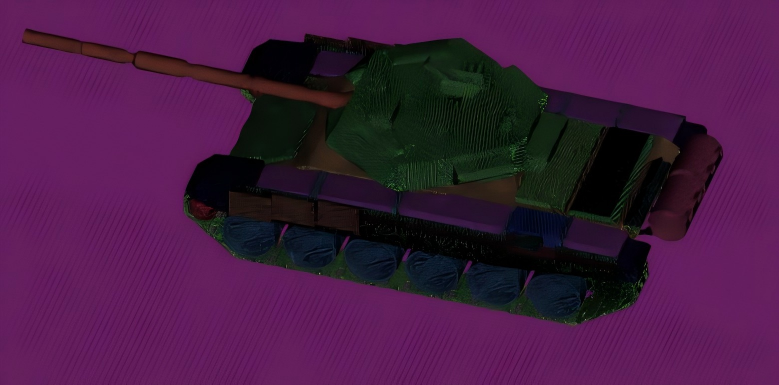
\includegraphics[width=0.46\textwidth]{Figures/FEM_Object_Grid_Example/Tank_Grid.png}
  \hfill
  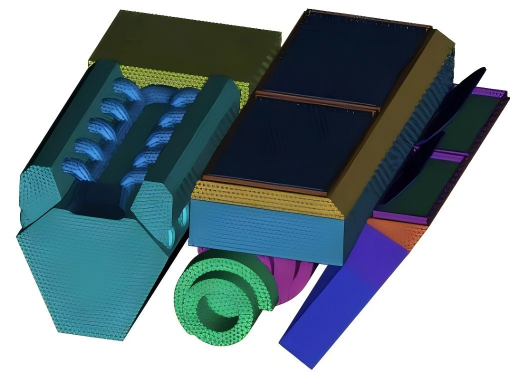
\includegraphics[width=0.46\textwidth]{Figures/FEM_Object_Grid_Example/Tank_Engine_Grid.png}
  \end{subcaptiongroup}
  \bicaption{红外仿真目标场景的三角形网格示例\cite{XuZhenDaoTanKeMuBiaoYuFuZaDiMianBeiJingOuHeReHongWaiTeZhengYanJiu2023}}{Example triangle meshes of infrared simulation target scenes~\cite{XuZhenDaoTanKeMuBiaoYuFuZaDiMianBeiJingOuHeReHongWaiTeZhengYanJiu2023}}
  \label{fig:fem_grid_example}

  \small
  坦克整车（左）与发动机舱部件（右）。
\end{figure}

\subsection{基于全局光照的辐射仿真方法}

1.2.2节的确定性数值方法将辐射视为网格单元间的热通量交换而非携带方向信息的光子输运，在处理复杂几何场景的多次反射与遮挡关系时受到根本制约，也难以融入光线追踪等计算机图形学方法体系。计算机图形学领域的全局光照技术——辐射度方法与光线追踪——为这一局限提供了解决思路；将其引入红外波段，可在不依赖角度离散的情况下高效处理几何复杂场景。\citeauthor{coiroGlobalIlluminationTechnique2013}较早在飞行器红外特征精确计算问题中将蒙特卡洛光线追踪全局光照模型集成至ONERA CRIRA仿真代码，采用Z缓冲器可见性判别、八叉树空间划分与重要性采样三重加速策略，实现了机身、进气道等部件间多重漫反射耦合的精确建模，证明了腔体部件的全局光照建模对辐亮度计算的影响可达$\pm$15\%\cite{coiroGlobalIlluminationTechnique2013}。

实时渲染需求推动了GPU加速红外仿真的快速发展。在辐射度精确渲染方向，\citeauthor{huangGPUbasedHighprecisionRealtime2014}通过有效平均值分解将谱耦合辐射方程转化为"原辐亮度$\times$有效平均因子"乘积形式，将多维参数预计算为三维GPU纹理查找表，实现了高精度实时辐射度渲染\cite{huangGPUbasedHighprecisionRealtime2014}；\citeauthor{wuRealtimeMidwavelengthInfrared2015}针对中波红外辐射仿真，提出了同时满足Helmholtz互易性与能量守恒约束的谱相关BRDF模型，构建了PRISSE集成仿真系统并通过实测光谱数据验证了其宽角度适用性\cite{wuRealtimeMidwavelengthInfrared2015}；\citeauthor{liRealtimeMultiresolutionRendering2018}针对超大规模地形背景，将遥感影像材质分类（$\kappa\approx0.9$）、简化能量平衡模型与15级多分辨率纹理金字塔结合，借助外存渲染技术实现了超过200~GB地形数据的无缝实时红外渲染\cite{liRealtimeMultiresolutionRendering2018}。

国内研究者在基于图形引擎的场景驱动方向进行了系统探索。\citeauthor{PanXuePingJiYuCreatorHeVegaDeHongWaiFeiXingShiJingFangZhen2007}利用Creator建模工具与Vega SensorVision传感器模块，结合预计算大气辐射传输查找表，构建了夜视飞行目标红外视景仿真系统\cite{PanXuePingJiYuCreatorHeVegaDeHongWaiFeiXingShiJingFangZhen2007}；\citeauthor{LinKaiJiYuOGREDeDongTaiHongWaiChangJingFangZhenYanJiu2010}在OGRE开源渲染引擎上整合"目标—背景—大气—成像系统"综合模型，在60~km$\times$60~km大场景下实现了82~fps实时双波段渲染，并以渲染合成器管线仿真了MTF、噪声和渐晕等成像效应\cite{LinKaiJiYuOGREDeDongTaiHongWaiChangJingFangZhenYanJiu2010}；\citeauthor{YangBoJiYuOSGDeHongWaiShiJingFangZhenYanJiu2017}在OSG引擎上提出了基于材质类别与相对高度的大规模地形动态分块调度方案，解决了空地导弹攻击场景下超大地形实时渲染的加载瓶颈\cite{YangBoJiYuOSGDeHongWaiShiJingFangZhenYanJiu2017}；\citeauthor{WangJunDiHaiMianHongWaiChangJingShengChengJiShuYanJiu2020}通过对实测光谱热特性数据的统计分析，系统化构建了地面车辆与海面舰船目标的全天候24小时红外场景生成系统\cite{WangJunDiHaiMianHongWaiChangJingShengChengJiShuYanJiu2020}；\citeauthor{LiWeiQingMianXiangShuZiLuanShengZhanChangDeHongWaiChangJingShiShiFangZhenFangFa2022}借助有限自动机对红外仿真计算流图进行并行化形式化分析，从理论上证明了多类原子并行结构的可行性，并构建了面向数字孪生战场样本生成的实时仿真系统\cite{LiWeiQingMianXiangShuZiLuanShengZhanChangDeHongWaiChangJingShiShiFangZhenFangFa2022}。

在与本文方法路线更为接近的高精度方向，\citeauthor{XuFeiFanJiYuOptiXBingXingGuangXianZhuiZongJiSuanDeHongWaiChengXiangFangZhenRuanJianYanZhi2022}将OptiX并行光线追踪与蒙特卡洛辐射传输相结合，引入Streaming RIS重要性采样策略与循环降噪自编码器，构建了支持中远红外双波段的高真实感仿真软件，验证了GPU硬件光追路线在红外成像仿真中的工程可行性\cite{XuFeiFanJiYuOptiXBingXingGuangXianZhuiZongJiSuanDeHongWaiChengXiangFangZhenRuanJianYanZhi2022}；\citeauthor{YuLiangYuJiYuLuJingZhuiZongDeSanWeiHongWaiChangJingFangZhenSuanFaJiShiXian2020}将蒙特卡洛路径追踪框架延伸至红外辐亮度积分与大气传输路径积分，通过OpenGL着色器实现GPU并行加速，是国内较早探索将路径追踪引入三维红外场景仿真的研究之一\cite{YuLiangYuJiYuLuJingZhuiZongDeSanWeiHongWaiChangJingFangZhenSuanFaJiShiXian2020}。

然而，上述基于全局光照的方法虽能有效处理辐射传输与光学遮挡，但无论渲染工具如何精进，热传导与热对流始终作为独立的预处理步骤通过温度场输入驱动辐射仿真，三种热输运机制从未在同一计算框架内统一建模。这种解耦从原理上限制了系统对动态热平衡、瞬态传热和材料内部热扩散的建模能力，也无法从路径空间角度对三种机制的耦合贡献进行统一采样与分析。

\subsection{基于路径追踪蒙特卡洛热输运仿真方法}
%% 写作思路：本节是文献综述的核心，直接支撑本文的方法论基础
%%   (1) 蒙特卡洛方法在热辐射中的早期应用
%%       - Howell (1964, 1969) 开创性工作 → \cite{howellMonteCarloSolution1964,howellApplicationMonteCarlo1969}
%%       - Kac (1947) 随机游走理论 → \cite{kacRandomWalkTheory1947}
%%   (2) 路径追踪在辐射传输中的发展
%%       - null-collision 方法 → \cite{galtierIntegralFormulationNullcollision2013}
%%       - Villefranque 等人的大气路径追踪 → \cite{villefranquePathtracingMonteCarlo2019,villefranqueTeapotCityParadigm2022}
%%   (3) 耦合热输运的蒙特卡洛框架（本文直接基础）
%%       - Fournier 等 (2016) 辐射-传导-对流耦合 → \cite{fournierRadiativeConductiveConvective2016}
%%       - Tregan 等 (2023) 辐射-传导耦合 → \cite{treganCouplingRadiativeConductive2023}
%%       - Bati 等 (2023, SIGGRAPH) 单路径空间耦合框架 + 红外渲染
%%         → \cite{batiCouplingConductionConvection2023}（本文最核心的基础文献）
%%       - Caliot 等 (2024) 城市尺度耦合 → \cite{caliotCoupledHeatTransfers2024}
%%   (4) 该方法的计算瓶颈分析
%%       - 每像素路径数多（高SPP需求）、路径内光追查询密集（每条路径~100次射线查询）
%%       - 递归/DFS 结构天然串行 → 引出对 GPU 加速和架构改造的需求
%%
%% [引用需求] Erturk (2017) 蒙特卡洛方法在辐射传输 → \cite{erturkMonteCarloMethods2017}
%% [引用需求] Fan 等 (2025) → \cite{fanMontecarlobasedSimulationsRadiative2025}
%% [引用需求] Mourtaday 等 (2024) → \cite{mourtadayMonteCarloSimulation2024}
%% [引用需求] 需补充：经典渲染领域的路径追踪文献（Kajiya 1986 渲染方程、Veach 1997 等）
%%            作为蒙特卡洛路径追踪在图形学侧的理论来源

针对上述辐射-传导-对流解耦建模的根本局限，将三种热输运机制纳入统一路径空间、以蒙特卡洛方法实现物理一致的耦合估计，成为近年来方法论层面的突破性探索方向。这一目标在方法论上根植于蒙特卡洛方法在热辐射领域的长期积累。

蒙特卡洛（Monte Carlo，MC）方法作为一类基于随机采样的数值计算方法，在热辐射领域有着悠久的应用历史。早在1947年，Kac 即从概率论角度建立了随机游走与热传导方程之间的理论联系\cite{kacRandomWalkTheory1947}。此后，Howell 等人率先将蒙特卡洛方法系统地应用于热辐射传输问题，开创了 MC 方法应用于辐射热仿真的先河，奠定了该领域的基础方法论\cite{howellMonteCarloSolution1964,howellApplicationMonteCarlo1969}。Erturk 等人对蒙特卡洛方法在辐射传输领域的应用进行了系统性综述，概括了其在辐射换热中的理论基础与工程应用\cite{erturkMonteCarloMethods2017}。

在计算机图形学领域，Kajiya 将光传输过程统一表述为渲染方程（Rendering Equation），为基于路径追踪的蒙特卡洛估计方法奠定了理论框架\cite{kajiyaRenderingEquation1986}。在辐射传输中处理非均匀介质时，Galtier 等人将 null-collision（零碰撞）方法引入积分形式的辐射传输方程，使蒙特卡洛方法在介质内部能够实现无偏的自由程采样\cite{galtierIntegralFormulationNullcollision2013}。Villefranque 等人将路径追踪方法拓展至城市尺度大气辐射传输仿真，揭示了该方法在复杂立体场景中优越的可扩展性与精度\cite{villefranquePathtracingMonteCarlo2019,villefranqueTeapotCityParadigm2022}。近年来，基于蒙特卡洛方法的辐射传输模拟在大气与建筑热环境仿真中持续取得进展\cite{mourtadayMonteCarloSimulation2024,fanMontecarlobasedSimulationsRadiative2025}。

将蒙特卡洛路径追踪推广至耦合热输运（辐射、传导、对流同时参与）是近年来方法论层面的重要突破。Fournier 等人构建了辐射-传导-对流三模式耦合的 MC 估计框架，首次在统一路径空间中同时表达三种热输运机制的耦合关系\cite{fournierRadiativeConductiveConvective2016}。Tregan 等人深化了辐射与传导耦合问题的路径估计器设计，发展了耦合条件下的高效采样策略\cite{treganCouplingRadiativeConductive2023}。Bati 等人在 SIGGRAPH 2023 提出了基于单一路径空间框架的耦合传导-对流-辐射蒙特卡洛算法，通过将随机游走（传导）、对流跳跃与辐射光线采样整合在同一路径结构内，实现了多物理耦合传热的物理一致无偏估计，并将该框架成功应用于红外热成像仿真，是本文工作最直接的方法论基础\cite{batiCouplingConductionConvection2023}。此后，Caliot 等人将该框架应用于城市尺度的耦合热传输仿真，进一步验证了其在大规模复杂场景下的适用性\cite{caliotCoupledHeatTransfers2024}。

然而，耦合热输运蒙特卡洛方法面临严峻的计算效率挑战。每幅红外图像需从数十万个像素独立追踪大量路径（每像素数百至数千条），每条路径内含有密集的光线-场景几何相交查询（每条路径约数十至上百次），且路径内部的逐条递归求解结构天然串行，难以在传统 CPU 多线程框架内充分并行化。这一计算瓶颈使得实际工程可用化的耦合 MC 仿真亟需高效的并行计算平台与架构支持，从而引出了本文研究的核心技术问题：如何将耦合热输运路径追踪仿真移植至 GPU 并行架构，在保证物理一致性的前提下，为耦合热输运求解提供面向 GPU 加速的架构基础。

\subsection{面向光线追踪的GPU并行加速技术}
%% 写作思路：综述 GPU 在科学计算和光线追踪中的加速发展
%%   (1) GPGPU / CUDA 并行计算概述——SIMT 执行模型、大规模线程并发
%%   (2) 光线追踪的 GPU 加速发展
%%       - 软件 BVH（Aila & Laine 2009 等）
%%       - Intel Embree（CPU SIMD 加速，作为本文 Baseline）→ \cite{EmbreeRayTracing}
%%       - NVIDIA RTX / RT Core 硬件加速（Turing 2018, Ampere 2020, Ada 2022）
%%       - OptiX / DXR / Vulkan RT 三大 API
%%   (3) Wavefront 执行模型在渲染中的应用
%%       - Laine 等 (2013) Megakernels vs Wavefront → 引出第三章思路
%%   (4) GPU 加速蒙特卡洛方法的现有工作
%%       - 指出现有 GPU MC 加速主要集中在可见光渲染
%%       - 耦合热输运的 GPU 加速尚无先例（强调本文贡献的新颖性）
%%
%% [引用需求] 需补充：CUDA/GPGPU 综述文献
%% [引用需求] Embree 论文 → \cite{EmbreeRayTracing,waldEmbreeKernelFramework2014}
%% [引用需求] OptiX 论文 → \cite{parkerOptiXGeneralPurpose2010}
%% [引用需求] Laine 等 Megakernels Considered Harmful → \cite{laineMegakernelsConsideredHarmful2013}
%% [引用需求] Aila & Laine GPU BVH 遍历 → \cite{ailaUnderstandingEfficiencyRay2009}
%% [引用需求] 需补充：RT Core 架构论文或 NVIDIA 技术白皮书

1.2.4节末已指出，耦合热输运蒙特卡洛方法面临严峻的计算效率挑战，根源在于路径的递归实现结构天然串行，阻断了跨路径批量积累查询的可能，无法有效利用GPU专用光追硬件的并行能力。解决这一瓶颈，需要理解近年来面向光线追踪的GPU并行加速技术的发展脉络。

图形处理器（GPU）自引入通用计算支持以来，已成为高性能并行计算的核心平台。以 NVIDIA CUDA 为代表的 GPGPU 编程框架以单指令多线程（SIMT）为核心执行模型，允许数千乃至数万个线程在单一 GPU 上同时调度执行，为蒙特卡洛等基于大量独立采样的算法提供了天然的并行扩展空间。与 CPU 的少核心高频率设计不同，GPU 以"宽而浅"的线程层次结构换取大规模数据并行吞吐量，特别适合路径追踪中大批量独立路径的并发计算。

光线追踪的 GPU 加速经历了从软件 BVH 遍历到专用硬件加速的演进。Aila 和 Laine 对 GPU 上层次包围体（BVH）遍历的执行效率进行了系统性分析，揭示了 GPU 光追的关键性能制约——线程束（warp）级的指令分歧（divergence）与不规则内存访问模式，为后续 GPU 光追架构优化提供了理论依据\cite{ailaUnderstandingEfficiencyRay2009}。在 CPU 端，Intel Embree 基于 SIMD 向量化技术实现了高度优化的光追内核，以极高的单核吞吐量成为 CPU 端光追的事实标准基准\cite{EmbreeRayTracing,waldEmbreeKernelFramework2014}。NVIDIA OptiX 是首个面向 GPU 的通用可编程光线追踪框架，提供了从场景几何管理、BVH 加速结构构建到光追着色器编程的完整接口，显著降低了 GPU 光追应用的开发门槛\cite{parkerOptiXGeneralPurpose2010}。2018 年随 Turing 架构推出的 RT Core 专用硬件单元，将 BVH 遍历和光线-三角形相交测试从着色器流水线剥离，作为独立硬件模块并行执行，使光追吞吐量获得数量级提升，后续 Ampere 与 Ada 架构延续并强化了这一设计。

在执行模型层面，Laine 等人深入分析了基于 GPU 的大内核（megakernel）方案的根本局限：路径追踪中各路径在每步计算中的着色逻辑高度分歧，统一内核内指令多样化导致 GPU 利用率严重下降。他们提出的 Wavefront 执行模型将渲染流水线拆分为多个细粒度着色内核，同类着色操作的路径在同一内核中批量执行，大幅改善了 GPU 占用率与内存访问局部性\cite{laineMegakernelsConsideredHarmful2013}。

GPU 加速蒙特卡洛方法在可见光渲染领域已有大量成熟工作，在国内红外仿真领域也出现了将 GPU 并行光追引入集成仿真系统的实践\cite{XuFeiFanJiYuOptiXBingXingGuangXianZhuiZongJiSuanDeHongWaiChengXiangFangZhenRuanJianYanZhi2022}。然而，现有工作均以辐射传输为主线，将热传导与对流作为解耦的预处理步骤，GPU 仅承担辐射光线查询任务。针对耦合热输运蒙特卡洛框架——辐射、传导、对流路径在单一随机游走中交织出现，求解器内部包含密集且类型多样的光追查询——的 GPU 并行化设计尚无文献报道。

值得说明的是，Wavefront 执行模型本身是成熟的 GPU 渲染架构。PBRT-v4\cite{pharrPhysicallyBasedRendering2023} 已在生产级 GPU 渲染器中实现了完整的 Wavefront 路径追踪管线。然而，耦合热输运路径追踪与可见光渲染 Wavefront 在三个维度上存在本质差异：(i)~路径需在辐射、传导、对流、界面耦合四类物理模块间动态切换，状态转移复杂度远超渲染中的材质-光源-介质三类着色器；(ii)~几何查询类型异构——除 RT 射线求交外，还包括最近面投影（CP）和封闭腔体成员判定（ENC）两类非光追查询，需在同一路径内混合调度；(iii)~路径生命周期跨数百至数千查询轮次（渲染路径通常仅 3\textasciitilde 30 步），持久化状态数据量大（约 3\textasciitilde 4 KB/路径），对 Cache 和显存的压力构成独特挑战。因此，将 Wavefront 架构应用于耦合热输运求解器需要全新的状态机设计、异构查询映射与路径池管理方案，这一空白构成了本文工作的核心技术创新空间。

\section{本文主要工作}
%% 写作思路：概括本文的研究内容和方法，突出创新点
%% [篇幅需求] 约1000字。
本文采用分阶段架构演进策略：首先通过 Wavefront 等价变换建立设备无关的批量查询接口，然后以 CPU-GPU 混合方式实例化该接口以验证架构正确性并定位性能关键路径——这正是本文标题所指的"混合架构"。该策略将物理正确性验证与极限性能优化解耦为两个独立目标，使本文得以在保证严格物理等价的前提下，精确定位性能瓶颈并为全 GPU 演进提供实验依据。

本文基于 Bati 等人\cite{batiCouplingConductionConvection2023}提出的蒙特卡洛耦合热输运算法框架，结合计算机图形学领域的 GPU 并行渲染与光线追踪加速技术，围绕"递归求解框架难以利用 GPU 硬件光追单元"这一核心瓶颈，开展以下三项研究工作。

（1）\textbf{基于有限状态机的 Wavefront 耦合热输运求解算法。}将递归求解过程中的全部几何查询调用点定义为挂起点，推导出路径状态机的完备设计约束与状态转换规则；通过递归到有限状态机的等价变换，将路径中间状态提取为持久化结构体，解耦状态推进与查询执行；在此基础上构建以持久化路径池为核心的 Wavefront 迭代模型，跨路径积累同类查询并批量提交，实现大规模并行几何查询。

（2）\textbf{三类异构几何查询的 GPU 等价映射方案。}射线最近命中查询由 RT Core 直接加速；场景最近点查询通过几何等价重构转化为等价光追形式；封闭腔体成员判定查询基于 Jordan--Brouwer 分离定理分解为上述两类查询的组合。三类映射整合于统一 GPU 查询管线，使耦合热输运求解中的全部几何查询均可利用专用光追硬件加速。

（3）\textbf{基于 \texttt{stardis-input} DSL 的图形化场景编辑器 StardisEditor。}作为面向仿真工作流的配套工程工具，求解器输入语言 \texttt{stardis-input} 采用严格位置编码格式，存在位置参数无标签、几何不可见、表面分区依赖外部工具等使用障碍。编辑器以该 DSL 的 BNF 形式文法驱动语法感知的解析与写出闭环，在此基础上提供三项 DSL 能力扩展：基于 VTK 的三维几何可视化、交互式画笔标注表面区域、图形化任务配置与队列化执行，通过 Cornell Box 耦合热仿真案例验证了完整闭环工作流。


\section{论文的组织结构}
%% 写作思路：概括论文的章节安排和内容，突出每章的核心贡献和相互之间的逻辑关系
%% [篇幅需求] 约800字。
本文共分为六章，内容安排如下：

第一章为绪论。本章介绍了热输运和红外仿真的研究背景，分析了国内外研究现状与发展脉络，指出现有方法的局限性和技术挑战，在此基础上提出了本研究的主要工作内容及组织架构。

第二章为相关理论与技术介绍。本章系统性地介绍了热输运与红外仿真课题所涉及的相关理论基础和技术方法。详细介绍了热输运的物理机制、数值求解方法和基于蒙特卡洛方法的热输运仿真框架。同时，介绍了GPU加速计算的原理和技术，以及相关的算法和实现方法，为后续章节的算法设计和实现提供理论支持。

第三章为基于 Wavefront 架构的并行化耦合热输运求解算法。本章针对基于路径追踪的蒙特卡洛热输运仿真方法的计算特点，在现有的蒙特卡洛耦合热输运仿真框架的基础上，剖析了该方法的计算瓶颈，并提出了一种基于 Wavefront 架构的并行化算法设计方案。该方法将递归求解器的递归结构展开为可调度的显式状态转移过程，并在此基础上实现了任务级并行调度框架，使计算任务能够以更细粒度被统一调度和分发。该方法立即解决了现有计算框架并行宽度受限于CPU线程数的根本问题，提升了并行宽度的拓展空间和调度灵活性，并为后续深度并行优化和计算设备拓展提供了架构基础。实验证明了该方法仅将光线追踪请求迁移至 GPU 中就可实现明显的加速，并分析了该方法的计算时间分布和潜在加速空间。

第四章为基于 OptiX 的硬件加速光追查询后端。面向 Wavefront 化的求解器所直接暴露的批量化查询需求，本章设计并实现了一个基于 NVIDIA OptiX 的 GPU 加速光追查询后端。该后端利用 GPU 的大规模并行计算能力和 RT Core 硬件加速功能，实现了高效的场景几何管理和光线追踪查询处理。实验结果显示，与基于 Intel Embree 的 CPU 查询后端相比，基于 OptiX 的 GPU 硬件加速查询后端在处理大批次光线查询实现了数百倍的极限吞吐量提升，并在实际仿真任务中实现了数倍的光追任务加速。

第五章为求解器场景编辑与仿真任务管理系统。本章以求解器输入语言 \texttt{stardis-input} 的 BNF 形式文法为基础，设计并实现图形化场景编辑器 StardisEditor。针对该 DSL 位置编码格式在几何不可见、表面分区与任务组装方面的系统性障碍，编辑器以文法规范驱动解析/写出闭环，并提供三项 DSL 能力扩展：基于 VTK 的三维几何可视化、交互式画笔标注表面区域、图形化任务配置与队列化执行。最后通过 Cornell Box 耦合热仿真案例验证了从场景构建到红外渲染输出的完整闭环工作流。

第六章为总结与展望。本章回顾并总结了本文的主要研究工作和贡献，分析了研究过程中存在的不足和局限性，并提出了未来的研究方向展望。

论文的整体组织架构如图\ref{fig:thesis-structure}所示。

\begin{figure}[htbp]
  \centering
  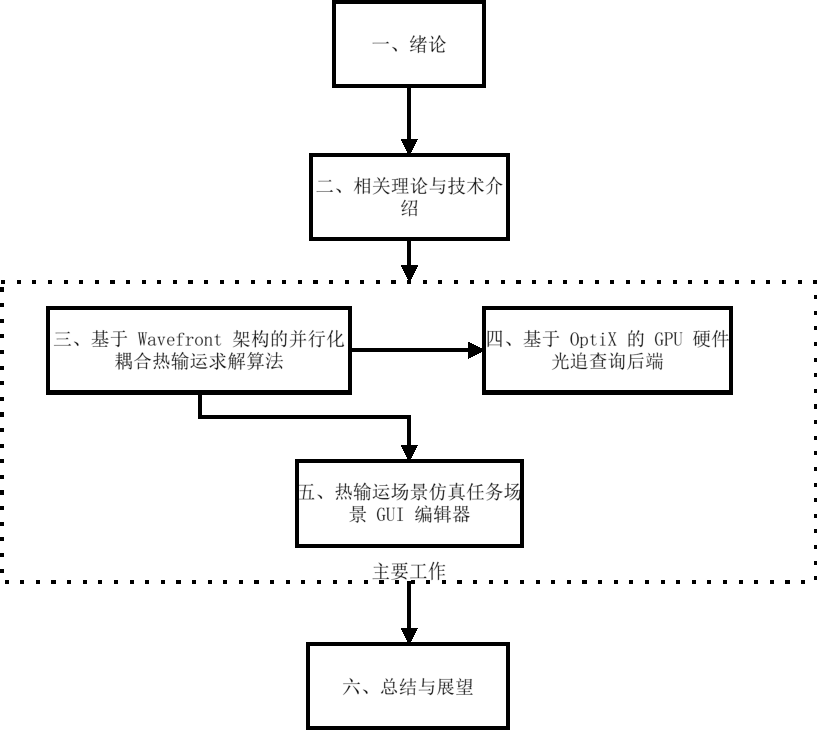
\includegraphics[width=0.95\textwidth]{Figures/ThesisArch/ThesisArch.pdf}
  \bicaption{论文整体组织架构图}{Overall Organization Structure of the Thesis}
  \label{fig:thesis-structure}
\end{figure}


%!TEX root = ../MainBody.tex

% 第二章
% ═══════════════════════════════════════════════════════════════════
% 写作思路（全章概要）：
%   本章是全文的理论根基，为第三~五章提供必要的知识铺垫。
%   与第一章文献综述的区别：第一章侧重"评述"（谁做了什么、各方法优劣），
%   本章侧重"阐述"（读者需要理解的具体理论和技术细节）。
%
%   每一节对应后续一章的理论基础：
%     2.1 热输运理论      → 支撑第三章求解器的物理模型
%     2.2 蒙特卡洛方法    → 支撑第三章求解器的数值方法
%     2.3 光追加速技术    → 支撑第四章 OptiX 后端
%     2.4 Wavefront 模型  → 支撑第三章并行化改造
% ═══════════════════════════════════════════════════════════════════
\chapter{相关理论与技术介绍}

\section{热输运理论}
%% [篇幅需求] 约1500字，重在建立物理直觉与数学符号约定，为后续蒙特卡洛求解铺垫。
%% [写作总思路]
%%   先分述三种基本热传递机制（各有独立小节），再集中讨论多机制耦合问题，
%%   最后以"现有数值方法难以高效耦合求解"作为动机，自然引出蒙特卡洛路径追踪统一框架。
%%   三种机制的篇幅按其在本文中的建模深度分配：传导 > 辐射 > 对流（对流建模最少，一段带过）。

\subsection{热传导}
%% 写作思路：
%%   - 物理机制：微观声子/自由电子碰撞传能，宏观上服从局域热平衡假设。
%%   - 傅里叶定律（本构关系）：$\mathbf{q} = -\lambda \nabla T$，说明各符号含义及导热系数 $\lambda$ 的各向同性假设。
%%   - 能量守恒推导热传导方程：$\rho c_p \frac{\partial T}{\partial t} = \nabla \cdot (\lambda \nabla T) + \dot{S}$，指出体积热源项 $\dot{S}$（辐射吸收在此处的耦合角色）。
%%   - 边界条件类型：Dirichlet（给定温度）、Neumann（给定热流）、Robin（辐射/对流混合边界）。
%%   - 【重点强调】在耦合热输运求解中，热传导是三种机制中最复杂、计算开销最大的部分，其主导地位体现在：
%%       (1) 偏微分方程维度高：热传导方程是三维抛物型 PDE，求解域为固体体积，而辐射仅涉及表面积分。
%%       (2) 蒙特卡洛求解代价高：基于随机游走（Brownian motion）的蒙特卡洛传导求解需大量短步长
%%           游走样本（步长与材料热扩散率、时间步相关），每步均需一次几何相交查询（判断是否撞到
%%           固体边界或进入不同材质区域），路径样本数远超其他路径。
%%       (3) 温度场更新瓶颈：整个求解迭代的收敛速度受制于固体内温度场的热传导弛豫时间，
%%           而非辐射或对流的边界交换速率。
%%     因此，加速几何相交查询对整体求解性能具有决定性作用，这也是本文引入 GPU 硬件光追的
%%     核心动机之一（详见第四章）。
%% [公式需求] 傅里叶定律、热传导方程（含时间项与稳态简化形式）
%% [引用需求] \cite{bergmanFundamentalsHeatMass2011}

热传导是固体介质中热量传递的基本方式。在微观层面，热传导依赖声子碰撞（非金属）和自由电子迁移（金属导体）实现能量转移；在宏观层面，当材料满足局域热平衡假设时，热流密度与温度梯度的关系由傅里叶定律（Fourier's Law）表达：
\begin{equation}
    \mathbf{q} = -\lambda \nabla T
    \label{eq:fourier}
\end{equation}
其中 $\mathbf{q}$（W/m²）为热流密度矢量，$\lambda$（W/(m·K)）为导热系数，$T$（K）为温度场。负号指出热量沿温度降低方向传递。对于各向同性均质材料，$\lambda$ 为标量；对于各向异性材质（如复合材料、晶体），则退化为二阶张量。

将傅里叶定律代入能量守恒方程，可推导出热传导方程：
\begin{equation}
    \rho c_p \frac{\partial T}{\partial t} = \nabla \cdot (\lambda \nabla T) + \dot{S}
    \label{eq:heat_conduction}
\end{equation}
其中 $\rho$（kg/m³）为材料密度，$c_p$（J/(kg·K)）为比热容，$\dot{S}$（W/m³）为体积热源项。在耦合热输运场景中，$\dot{S}$ 包含辐射被固体吸收所转化的热源及其他内热源。对稳态问题，方程左端时间导数项为零，退化为泊松方程 $\nabla \cdot (\lambda \nabla T) + \dot{S} = 0$。

热传导方程的求解需配合以下边界条件之一：
\begin{itemize}
    \item 第一类（Dirichlet）边界：直接给定边界温度 $T|_{\partial\Omega} = T_w$，例如固体壁面与恒温热源直接接触，壁面温度由热源温度直接确定。
    \item 第二类（Neumann）边界：给定法向热流 $-\lambda \nabla T \cdot \hat{n}|_{\partial\Omega} = q_w$，例如绝热边界（$q_w = 0$，无热流穿过）或已知外加热流密度的加热面。
    \item 第三类（Robin）边界：联立温度与热流，典型形式为辐射-对流混合边界条件，例如固体外壁面同时受到对流冷却与辐射散热，热流由表面温度通过换热系数和 Stefan-Boltzmann 定律共同确定。
\end{itemize}

在本文的耦合热输运求解框架中，热传导是三种机制中计算开销最大、地位最为核心的部分，这一主导性体现在三个层面：其一，热传导方程是三维抛物型偏微分方程，求解域为整个固体体积，而热辐射仅涉及表面积分，体积求解的空间维度远高于后者；其二，在蒙特卡洛路径追踪框架中（详见第 2.2 节），传导路径通过三维布朗随机游走逼近，需要大量短步长采样，每步均需一次几何相交查询以判断游走粒子是否触及固体边界或跨越材质界面，路径样本总量远超辐射路径；其三，耦合迭代的整体收敛速度受制于固体温度场的热传导弛豫时间常数，而非辐射或对流的边界交换速率。上述特点决定了：大批量几何相交查询的吞吐能力是制约整体仿真性能的关键瓶颈，这也构成了本文引入 GPU 硬件光线追踪加速的核心动机之一。

\subsection{热辐射}
%% 写作思路：
%%   - 物理机制：电磁波辐射传能，不需要介质接触，是红外仿真的主导机制。
%%   - 黑体辐射基础：普朗克分布、Stefan-Boltzmann 定律 $E_b = \sigma T^4$、Kirchhoff 定律（发射率=吸收率）。
%%   - 辐射传输方程（RTE）：沿射线方向 $\hat{\omega}$ 的强度变化，含自发发射、吸收、散射项：
%%         $\hat{\omega} \cdot \nabla L = \kappa (L_b - L) - \sigma_s L + \frac{\sigma_s}{4\pi} \int_{4\pi} L(\hat{\omega}') \, d\hat{\omega}'$
%%   - 实际工程场景：表面辐射（漫射灰体假设）是本文主要考虑的情形，介质散射暂不讨论。
%% [公式需求] Stefan-Boltzmann 定律、Kirchhoff 定律、辐射传输方程 (RTE) 微分形式
%% [引用需求] \cite{modestRadiativeHeatTransfer2013,howellThermalRadiationHeat2021}

热辐射以电磁波形式传递能量，无需介质接触即可在真空中远距离传播，是红外仿真场景中的重要传热机制。理想黑体是最完美的辐射源，其半球辐射力由 Stefan-Boltzmann 定律给出：
\begin{equation}
    E_b = \sigma T^4
\end{equation}
其中 $\sigma = 5.67 \times 10^{-8}$ W/(m²·K$^4$) 为 Stefan-Boltzmann 常数。实际工程材料为灰体，辐射力通过发射率 $\varepsilon \in [0,1]$ 修正为 $E = \varepsilon \sigma T^4$。根据 Kirchhoff 定律，在热平衡条件下材料的光谱发射率等于光谱吸收率（$\varepsilon_\lambda = \alpha_\lambda$），这为仿真中材料参数的统一描述提供了依据。

在参与性介质中，辐射强度 $L$（W/(m²·sr)）沿传播方向 $\hat{\omega}$ 的变化由辐射传输方程（Radiative Transfer Equation，RTE）描述：
\begin{equation}
    \hat{\omega} \cdot \nabla L(\mathbf{x}, \hat{\omega})
    = \kappa\bigl[L_b(T) - L(\mathbf{x}, \hat{\omega})\bigr]
    - \sigma_s L(\mathbf{x}, \hat{\omega})
    + \frac{\sigma_s}{4\pi} \int_{4\pi} L(\mathbf{x}, \hat{\omega}') \, \mathrm{d}\hat{\omega}'
    \label{eq:rte}
\end{equation}
其中 $\kappa$（m$^{-1}$）为吸收系数，$\sigma_s$（m$^{-1}$）为散射系数，$L_b(T) = \sigma T^4/\pi$ 为黑体辐射强度。方程右侧三项依次对应热发射引起的强度增益、出散射引起的强度衰减，以及来自其他方向的入散射能量补偿。

本文聚焦于不透明固体表面之间的辐射换热，采用漫射灰体（diffuse-gray）假设：表面辐射各向同性，材料发射率与波长无关。在此简化下，固体间介质视为透明（$\kappa = \sigma_s = 0$），RTE 退化为纯直线传播问题——辐射强度在两次表面碰撞之间沿直线保持不变，辐射传输仅需追踪光线的几何可见性。这一特性使光线追踪成为求解此类辐射传输的天然工具。此处，$\kappa > 0$ 或 $\sigma_s > 0$ 的介质称为参与性介质（participating media），其对立面即为上述透明介质假设。

表面辐射特性的完整描述采用双向反射分布函数（Bidirectional Reflectance Distribution Function，BRDF）$f_r(\hat\omega_i, \hat\omega_o) = \mathrm{d}L_o(\hat\omega_o) / \mathrm{d}E_i(\hat\omega_i)$（单位 sr$^{-1}$），定义为出射辐射亮度与入射辐照度之比\cite{modestRadiativeHeatTransfer2013,howellThermalRadiationHeat2021}。工程热辐射中最常用的简化模型为Lambert（漫射）反射，此时 $f_r = \rho_d / \pi$，$\rho_d = 1 - \varepsilon$ 为漫反射率。本文与 Bati 等人\cite{batiCouplingConductionConvection2023}相同，采用 Lambert 反射模型。

\subsection{热对流}
%% 写作思路（篇幅精简，约100字正文）：
%%   - 简述物理机制：流体宏观运动携带热量，固-流界面产生对流换热。
%%   - 牛顿冷却定律：$q = h(T_s - T_\infty)$，对流换热系数 $h$ 是综合了流场信息的集总参数。
%%   - 直接说明本文的建模立场：本文不求解 Navier-Stokes 方程，对流仅作为边界条件（CNV 过程）
%%     出现——给定预计算或用户指定的 $h$ 值，在固体表面施加对流热损失。
%%     这是工程热仿真中的标准解耦简化，将对流的复杂流场问题与热传导/辐射求解解耦，
%%     不影响本文所关注的辐射传热建模精度。
%% [公式需求] 牛顿冷却定律（一行即可）
%% [引用需求] \cite{bergmanFundamentalsHeatMass2011}

热对流通过流体的宏观运动携带热量，是固体壁面与流体环境之间重要的热交换方式。固-流界面处的对流换热通常以牛顿冷却定律（Newton's Law of Cooling）建模：
\begin{equation}
    q_\mathrm{conv} = h\,(T_s - T_\infty)
\end{equation}
其中 $q_\mathrm{conv}$（W/m²）为对流热流密度，$T_s$ 与 $T_\infty$ 分别为固体表面温度和远场流体温度，$h$（W/(m²·K)）为对流换热系数，综合了边界层厚度、流速、流体热物性等流场信息。

本文不求解 Navier-Stokes 方程，对流以简化的边界条件（CNV 过程）形式参与耦合求解：对流换热系数 $h$ 是一个场景相关的自定义常量，在固体表面施加对应的热损失约束\cite{bergmanFundamentalsHeatMass2011}。Bati 等人\cite{batiCouplingConductionConvection2023}的耦合框架同样采用此简化——将对流以 Newton 冷却定律形式纳入边界条件，$h$ 为用户输入的经验参数。

$h = \text{const}$ 假设的适用性可通过 Biot 数 $\text{Bi} = hL_c/k$ 评估，其中 $L_c$ 为固体特征长度、$k$ 为固体导热系数。当 $\text{Bi} \ll 1$ 时，固体内部温度梯度远小于固-流界面温差，表面温度近似均匀，恒定 $h$ 即可充分描述对流热交换\cite{bergmanFundamentalsHeatMass2011}。该条件在薄壁高导热金属结构（如铝合金薄板、散热翅片）中广泛成立。对于 $\text{Bi} \gg 1$ 的场景（厚壁低导热体或高速气流），$h$ 的空间变化不可忽略，需引入局部 $h(\mathbf{x})$ 分布或直接耦合 CFD 流场求解。本文验证场景均满足 $\text{Bi} < 0.1$ 的集总参数适用条件。

这是工程热仿真中标准的解耦简化策略，适用于强制对流或已知经验关联式的场景；对于自然对流或强烈耦合的流-热问题，则需要 Navier-Stokes 方程的完整求解。

\subsection{多机制耦合热输运}
%% 写作思路：
%%   - 说明三种机制在实际工程场景（如飞行器舱体热防护、红外特征预测）中同时存在，不可单独求解。
%%   - 耦合形式：
%%       (a) 边界耦合：固-流-辐射三者联立的能量平衡边界条件（表面温度由三者共同决定）：
%%             $-\lambda \nabla T \cdot \hat{n} + h(T_s - T_\infty) + \varepsilon \sigma T_s^4 - \alpha G = 0$
%%       (b) 体积耦合：半透明介质中辐射吸收项 $\dot{S}$ 直接作为热传导方程的体热源。
%%   - 耦合带来的数值挑战：非线性（$T^4$ 项）、各机制时间尺度差异大、分区网格难以统一。
%%   - 引出动机：本文采用蒙特卡洛路径追踪在统一的路径空间中描述三种机制，自然处理耦合边界，
%%     避免了传统方法的跨模块耦合迭代。
%%   - 引出 GPU 加速动机（此处埋伏笔，2.3~2.4 展开）：三种机制统一在同一路径空间后，
%%     所有过程（RAD/BND/CND/CNV）大量依赖几何射线查询；这些查询在形式上是同构的
%%     （相同的 API、相同的数据布局），天然适合批量化并行，促成了将射线查询卸载到 GPU
%%     硬件光追单元（RT Core）的设计动机。计算量最大的部分是固体内热传导产生的大量随机游走
%%     路径，这些路径同样通过几何相交（判断是否到达固体边界）来驱动前进，因此加速几何查询
%%     对整体求解效率有决定性影响。
%% [公式需求] 联合边界条件方程、体积耦合能量方程
%% [引用需求] \cite{batiCouplingConductionConvection2023,howellThermalRadiationHeat2021}

在实际工程场景中，上述三种热传递机制往往同时发生并相互影响，不可单独求解。以飞行器外壁面热防护与红外特征预测为典型案例\cite{modestRadiativeHeatTransfer2013}：固体结构通过热传导将内部热量向外传递，外壁面向外辐射红外能量，同时受到气流的对流冷却。三种机制在固-流界面处的耦合通过联合能量平衡边界条件联立约束：
\begin{equation}
    -\lambda \nabla T \cdot \hat{n}\big|_{\partial\Omega}
    + h\,(T_s - T_\infty)
    + \varepsilon\sigma T_s^4
    - \alpha G
    = 0
    \label{eq:coupled_bc}
\end{equation}
其中 $G$（W/m²）为投射辐照度，即到达该表面的外部辐射通量，$\alpha$ 为表面吸收率。式\,\eqref{eq:coupled_bc} 表明，固体表面温度 $T_s$ 由传导热流、对流热损失和净辐射热流共同决定，三者之间因 $T_s^4$ 项存在高度非线性耦合。

对于含半透明固体的场景，还存在体积耦合：辐射在固体内部被吸收，转化为体积热源
\begin{equation}
    \dot{S} = \kappa \int_{4\pi} L \, \mathrm{d}\hat{\omega} - 4\kappa \sigma T^4
\end{equation}
直接作为热传导方程\,\eqref{eq:heat_conduction} 中的源项 $\dot{S}$，使辐射场与温度场在体积内互相依存。

耦合热输运问题的数值求解面临多重挑战：边界条件中的 $T^4$ 非线性项使方程组高度非线性，需要迭代求解；三种机制的特征时间尺度跨越多个数量级（辐射以光速传播，传导弛豫时间从秒到小时）；以及各机制在传统数值方法中通常依赖不同的网格离散形式——热传导采用三维体积有限元或有限差分网格\cite{bergmanFundamentalsHeatMass2011}，辐射采用表面网格（角系数法）或体积网格加角度离散（离散坐标法，DOM\cite{fivelandDiscreteOrdinatesSolutions1984}），对流则依赖流体域有限体积网格——耦合迭代需要在这些异构网格间进行物理量的插值传递，引入额外的数值误差与实现复杂度。例如，Kottler 等人\cite{kottlerPhysicallybasedThermalSimulation2019}采用统一的有限体积网格同时求解传导与对流，辐射则以标量天空视角因子通量项形式注入能量方程——各机制虽共享同一网格，但辐射仅计算外表面与天空的单次交换，无面间互反射、无 BRDF；这种"分别建模、通量求和"的做法在工程实践中具有代表性，但当场景存在多腔体互反射或复杂几何遮挡时，辐射精度受限。

为克服上述困难，Bati 等人\cite{batiCouplingConductionConvection2023}提出了蒙特卡洛路径追踪耦合求解框架，在统一的路径空间中同时描述辐射、传导与对流三种机制——路径在介质界面处依据物理规律发生机制转换，自然处理耦合边界条件，无需在不同求解器之间迭代传递耦合量。本文基于该框架设计并实现求解器（详见 \ref{sec:coupled_framework}），并针对其在工程部署中的计算效率问题进行架构层面的加速优化（第三、四章）。三种机制统一于同一路径空间还带来了额外优势：所有过程（辐射传播、界面事件判断、传导随机游走、对流边界处理）均大量依赖几何射线查询，且这些查询在接口形式上完全同构，天然适合批量化并行，为将几何查询卸载至 GPU 硬件光追单元（RT Core）奠定了基础。

\paragraph{假设与简化说明。}
本文的工程实现与Bati等人\cite{batiCouplingConductionConvection2023}的核心算法共享以下5条简化假设（Bati 原文称为 Constraints 1--5）：(1) 固体不透明、流体透明——固体内无辐射传输，辐射在流体中沿直线传播；(2) 流体元完全混合——各流体元假设等温，温度由 Newton 冷却律参数化；(3) 各子域物理参数（$k$、$\varepsilon$、$h$ 等）均匀恒定；(4) 所有参数场预先给定，不由求解器自身计算；(5) 辐射换热系数 $h_R = 4\sigma\varepsilon\theta_\text{ref}^3$ 按参考温度线性化。上述简化是红外仿真工程实践中的常见选取\cite{howellThermalRadiationHeat2021}，缩小了实现规模但不影响本文所提出的并行化架构加速方法的普适性。

\section{蒙特卡洛热输运求解方法}
%% [篇幅需求] 约2500字，从基础原理逐步深入到本文具体实现，是全章核心节。
%% [写作总思路]
%%   先建立蒙特卡洛方法的通用数学基础（2.2.1），再介绍其在热辐射领域的早期应用（2.2.2），
%%   然后引入路径追踪的现代表述（2.2.3），重点阐述 Bati 等人将三种机制统一在单个路径空间的
%%   核心框架（2.2.4），最后以代码层面描述原始 CPU 求解器的 DFS 实现（2.2.5），
%%   为第三章的改造工作提供直接对照物。

\subsection{蒙特卡洛积分方法}
%% 写作思路：
%%   - 核心思想：用随机样本的经验均值估计积分期望：
%%         $\hat{I}_N = \frac{1}{N} \sum_{i=1}^{N} \frac{f(x_i)}{p(x_i)}$，方差以 $O(N^{-1/2})$ 收敛。
%%   - 重要性采样：选取 $p(x) \propto |f(x)|$ 最小化方差，说明在多维积分中相对确定性方法的优势
%%     （维数灾难无关，复杂度仅随维数线性增长）。
%%   - 物理可解释性：热输运中每条"路径"就是一个样本，其贡献权重即估计量 $f(x)/p(x)$。
%% [公式需求] 蒙特卡洛积分估计量、方差公式、重要性采样估计量
%% [引用需求] \cite{howellMonteCarloSolution1964}（最早将 MC 引入热辐射的文献，可在此处引用作历史溯源）

蒙特卡洛方法的核心思想是将高维积分问题转化为概率期望的估计问题。设需计算积分
\begin{equation}
    I = \int_\Omega f(\mathbf{x}) \, \mathrm{d}\mathbf{x}
    \label{eq:mc_integral}
\end{equation}
其中 $\Omega \subseteq \mathbb{R}^d$ 为积分域。蒙特卡洛方法在 $\Omega$ 上按概率密度函数 $p(\mathbf{x})$ 独立采样 $N$ 个随机样本 $\{\mathbf{x}_i\}_{i=1}^N$，构造如下蒙特卡洛估计量：
\begin{equation}
    \hat{I}_N = \frac{1}{N} \sum_{i=1}^{N} \frac{f(\mathbf{x}_i)}{p(\mathbf{x}_i)}
    \label{eq:mc_estimator}
\end{equation}
由大数定律，$\hat{I}_N$ 是 $I$ 的无偏估计（$E[\hat{I}_N] = I$），其误差标准差随样本量增大以 $O(1/\sqrt{N})$ 收敛，这一速率与积分维数 $d$ 无关。相比之下，确定性数值积分方法（如 Gauss 求积\cite{modestRadiativeHeatTransfer2013}）对 $d$ 维积分问题需要 $O(\epsilon^{-d})$ 个采样点才能达到误差 $\epsilon$，计算量随维数指数增长——这一困难通常称为维数灾难（curse of dimensionality）。在路径追踪语境中，路径的每一次随机决策（方向采样需 2 个随机数、位置采样需 1 个随机数、界面模态分叉需 1 个随机数）都对应积分的一个维度；一条经历 $n$ 次弹射的耦合路径涉及约 $2n$--$3n$ 维积分空间，典型场景中路径弹射次数为数十至数百次，远超确定性方法可实际处理的范围（通常 $d > 10$ 即不实际）。蒙特卡洛方法的 $O(1/\sqrt{N})$ 维数无关收敛性正是其在此类高维积分问题中广泛应用的根本原因。

由方差的线性性质与估计量的独立同分布假设可直接推导\cite{modestRadiativeHeatTransfer2013}，估计量的方差为：
\begin{equation}
    \mathrm{Var}[\hat{I}_N] = \frac{1}{N} \left[ \int_\Omega \frac{f(\mathbf{x})^2}{p(\mathbf{x})} \, \mathrm{d}\mathbf{x} - I^2 \right]
    \label{eq:mc_variance}
\end{equation}
为降低方差，可引入重要性采样（Importance Sampling）策略：选取与被积函数幅度正比的采样分布 $p(\mathbf{x}) \propto |f(\mathbf{x})|$，使比值 $f(\mathbf{x})/p(\mathbf{x})$ 接近常数，从而使式\,\eqref{eq:mc_variance} 中方括号内的积分项趋近 $I^2$，方差趋于零。在热输运蒙特卡洛求解中，每条随机路径对应一个样本 $\mathbf{x}_i$，其对积分量（如探测器辐亮度）的贡献权重即为 $f(\mathbf{x}_i)/p(\mathbf{x}_i)$。需要指出的是，本文所采用的 Bati 等人耦合框架并未引入人为设计的重要性采样分布\cite{batiCouplingConductionConvection2023}，而是通过物理概率的精确参数化使路径权重天然保持为单位值（详见 \ref{sec:coupled_framework}）。

\subsection{热辐射的蒙特卡洛求解}
%% 写作思路：
%%   - 经典做法（正向追踪）：从热源发射能量包（energy bundle），追踪其在场景中的吸收、反射，
%%     统计各表面的能量沉积以计算辐射热流。
%%   - Howell (1964) 的奠基性工作：首次系统地将 MC 应用于辐射传热计算。
%%   - 局限性：正向追踪对复杂场景收敛慢（能量包难以准确击中观测面），引出反向路径追踪的动机。
%% [公式需求] 辐射交换因子（view factor）的 MC 估计
%% [引用需求] \cite{howellMonteCarloSolution1964,howellThermalRadiationHeat2021}

蒙特卡洛方法最早由 Howell\cite{howellMonteCarloSolution1964,howellApplicationMonteCarlo1969}系统地引入辐射传热领域，奠定了热辐射数值计算的随机方法论基础。其经典做法为正向蒙特卡洛追踪（Forward MC Tracing）：从热辐射源面出发，以与黑体辐射力 $\sigma T^4$ 正比的概率发射离散能量包（energy bundle），逐步追踪每个能量包在场景中的漫反射与吸收过程，并将最终被各表面吸收的能量累积为辐射热流。

工程辐射计算的核心参数为辐射角系数（view factor）$F_{ij}$，其定义为从漫射表面 $i$ 出发的辐射能量中被表面 $j$ 所拦截的比例：
\begin{equation}
    F_{ij} = \frac{1}{A_i} \int_{A_i} \int_{A_j}
    \frac{\cos\theta_i \cos\theta_j}{\pi r^2} \, V(\mathbf{x}_i, \mathbf{x}_j)
    \, \mathrm{d}A_j \, \mathrm{d}A_i
    \label{eq:view_factor}
\end{equation}
其中 $\theta_i$、$\theta_j$ 分别为两点连线方向与各自表面法向的夹角，$r$ 为两点间距，$V(\mathbf{x}_i, \mathbf{x}_j) \in \{0, 1\}$ 为几何可见性函数（被遮挡时为零）。该双重曲面积分的解析形式仅在少数规则几何下存在；蒙特卡洛方法从表面 $i$ 按余弦加权方向均匀发射 $N$ 条射线，统计命中表面 $j$ 的数量 $N_{ij}$，可给出无偏估计 $\hat{F}_{ij} = N_{ij}/N$，适用于任意复杂场景几何。

然而，正向追踪存在显著的效率局限：在复杂场景中，从热源发射的能量包难以精确命中面积较小的观测面（如红外探测器像素），导致大量样本对目标量无贡献，收敛缓慢。这一问题促使后续研究转向反向路径追踪（backward path tracing）策略\cite{kajiyaRenderingEquation1986}——从观测面出发沿光路反向追踪，天然聚焦于对观测有贡献的路径，是本文求解器所采用的核心追踪策略。

\subsection{路径追踪方法}
%% 写作思路：
%%   - 渲染方程（Kajiya 1986）：将辐射亮度表达为递归积分方程
%%         $L_o(\mathbf{x}, \hat{\omega}_o) = L_e(\mathbf{x}, \hat{\omega}_o) + \int_\Omega f_r(\mathbf{x}, \hat{\omega}_i, \hat{\omega}_o) L_i(\mathbf{x}, \hat{\omega}_i) (\hat{\omega}_i \cdot \hat{n}) \, d\hat{\omega}_i$
%%   - 路径积分表述：将递归展开为路径空间上的高维积分，MC 采样即为随机生成路径。
%%   - 反向路径追踪（eye path tracing）：从传感器（相机/探测器）出发，每次弹射追踪一条路径，
%%     自然地只计算对观测有贡献的路径，适合红外成像仿真（每个像素对应一个积分估计）。
%%   - null-collision 技术：在参与介质中使用虚拟碰撞均匀化消光系数，消除条件分支，
%%     使 MC 路径在介质中的步进无偏且实现简单。
%% [公式需求] 渲染方程、路径空间测度、null-collision 的均匀消光表达
%% [引用需求] \cite{kajiyaRenderingEquation1986,galtierIntegralFormulationNullcollision2013}

Kajiya（1986）\cite{kajiyaRenderingEquation1986}在计算机图形学领域提出的渲染方程（Rendering Equation）为路径追踪提供了严格的数学基础。渲染方程将空间一点 $\mathbf{x}$ 沿方向 $\hat{\omega}_o$ 的出射辐射亮度表达为自发射项与半球积分入射亮度之和：
\begin{equation}
    L_o(\mathbf{x}, \hat{\omega}_o) = L_e(\mathbf{x}, \hat{\omega}_o) +
    \int_{\mathcal{H}^2} f_r(\mathbf{x}, \hat{\omega}_i, \hat{\omega}_o) \,
    L_i(\mathbf{x}, \hat{\omega}_i) \, |\hat{\omega}_i \cdot \hat{n}| \, \mathrm{d}\hat{\omega}_i
    \label{eq:rendering}
\end{equation}
其中 $f_r$（sr$^{-1}$）为双向反射分布函数（BRDF，2.1.2 已定义），描述表面将入射方向的辐射重新分配到出射方向的能力；$\mathcal{H}^2$ 为上半球立体角域，$\hat{n}$ 为表面法向。由于 $L_i$ 中包含对上一次碰撞点出射亮度的递归依赖，将渲染方程逐层展开可得到路径空间上的高维积分——路径追踪即通过蒙特卡洛方法在该路径空间上随机采样，给出积分的无偏估计。

\textbf{反向路径追踪}（backward path tracing）从传感器（像素/探测器）出发，沿反向光路逐次弹射：在每次碰撞点处，按 BRDF 采样分布随机选取新方向 $\hat{\omega}_i$，路径权重乘以对应的 $f_r / p(\hat{\omega}_i)$ 因子，直至路径被光源/热源终止，或通过俄罗斯轮盘赌（Russian roulette）以概率 $1 - \min(W/W_0, 1)$ 无偏截断。这种策略将计算集中在对观测像素有贡献的路径上，图像中的每个像素对应一个独立的蒙特卡洛积分估计，构成了一个可行的工程实践方案。

在参与性介质（含散射或吸收的气体/颗粒场，本文工程实现中简化为透明介质，参见 2.1.2 及 2.1.4 末尾假设说明）中，路径步进需处理非均匀的消光系数。Null-collision 技术\cite{galtierIntegralFormulationNullcollision2013}（也称 Woodcock 追踪）通过引入虚拟碰撞粒子，将非均匀消光场均匀化为虚构上界 $\bar{\mu}_t = \max_{\mathbf{x}} \mu_t(\mathbf{x})$，并定义 null-collision 系数：
\begin{equation}
    \mu_n(\mathbf{x}) = \bar{\mu}_t - \mu_t(\mathbf{x}) \geq 0
    \label{eq:null_collision}
\end{equation}
在均匀消光 $\bar{\mu}_t$ 下，自由程服从参数为 $\bar{\mu}_t$ 的指数分布，便于直接采样。路径到达每一碰撞点后，以概率 $\mu_n/\bar{\mu}_t$ 视为虚碰撞（不改变方向，继续传播），以概率 $\mu_s/\bar{\mu}_t$ 发生散射，以概率 $\mu_a/\bar{\mu}_t$ 发生吸收，从而消除步进中的非均匀条件分支，实现无偏且简洁的介质内路径追踪。

Null-collision 的接受/拒绝机制具有超越参与性介质的普适性。在耦合热输运求解中，界面处三模态概率（\ref{sec:coupled_framework}）的归一性依赖于线性化辐射换热系数 $h_R$ 的准确性；当去除线性化假设时，$h_R$ 依赖未知温度 $\theta$，三概率无法预先确定，此时 Null-collision 的接受/拒绝采样可恢复估计量的无偏性（详见 \ref{sec:coupled_framework}）。

\subsection{单路径空间耦合求解框架}
\label{sec:coupled_framework}
%% 写作思路：
%%   - 核心贡献（Bati et al. 2023）：将传导、对流、辐射三种机制统一为"广义路径"，
%%     在单个路径空间中构造无偏估计量，路径在不同介质/界面处自然发生机制转换。
%%   - 三类路径段：
%%       · 辐射段（RAD）：光子在真空/透明介质中直线传播，Fermat 折射；
%%       · 传导段（CND）：热量在固体内随机游走（Brownian motion），由 Kac 公式关联到 Green 函数；
%%       · 对流段（CNV）：以边界条件形式在固-流界面处执行能量转移，路径终止或分叉。
%%   - 耦合事件：路径在固-气界面（BND 过程）以概率分叉：以发射率概率进入辐射段，
%%     以 $(1-\varepsilon)$ 概率继续传导段，以对流换热权重转移给对流段。
%%   - 路径权重的递推形式：每次事件乘以对应的 BRDF/透过率/换热权重，最终贡献到探测器像素。
%%   - 本文实现的简化：仅实现一阶 Picard 迭代（线性化处理 $T^4$ 非线性项），
%%     传导段采用有限元/有限差分离散代替随机游走（直接数值求解 Fourier 方程作为底层支撑）。
%% [公式需求] 耦合路径的估计量定义、Kac 公式 $u(x) = E_x[g(B_\tau)]$
%% [图表需求] 耦合路径示意图——一条路径经历 RAD→BND→CND→BND→RAD 各段的切换示意
%% [引用需求] \cite{batiCouplingConductionConvection2023,treganCouplingRadiativeConductive2023,fournierRadiativeConductiveConvective2016}

Bati 等人（2023）提出了将辐射、传导、对流三种热传递机制统一到单一路径空间的蒙特卡洛耦合求解框架\cite{batiCouplingConductionConvection2023}，这也是本文求解器的理论基础。该框架的核心思想在于：不再为各机制分别建立独立的方程组并通过跨求解器迭代传递耦合量，而是保留各机制内部的物理方程描述（传导仍由傅里叶方程驱动，辐射仍沿直线传播），仅在介质界面处通过概率分叉实现机制间的转换——路径在抵达固-流或固-固界面时，按界面物理参数决定的概率随机选择进入下一种传热机制的路径段，在同一路径空间中构造对目标量（如探测器辐亮度）的无偏蒙特卡洛估计量。在路径追踪语境下，2.1 所述的三种传热机制被视为路径的三种传热模态（heat transfer mode，Bati 等人\cite{batiCouplingConductionConvection2023}原文用语）——路径的当前模态决定了其物理行为（传导模态下执行布朗游走、辐射模态下沿直线传播、对流模态下采样流体温度），路径在界面处发生模态转换。后续章节中"模态"均指此含义。\cref{fig:coupled_path_meta}展示了四个物理模块之间的模态转换关系。

\begin{figure}[htbp]
  \centering
  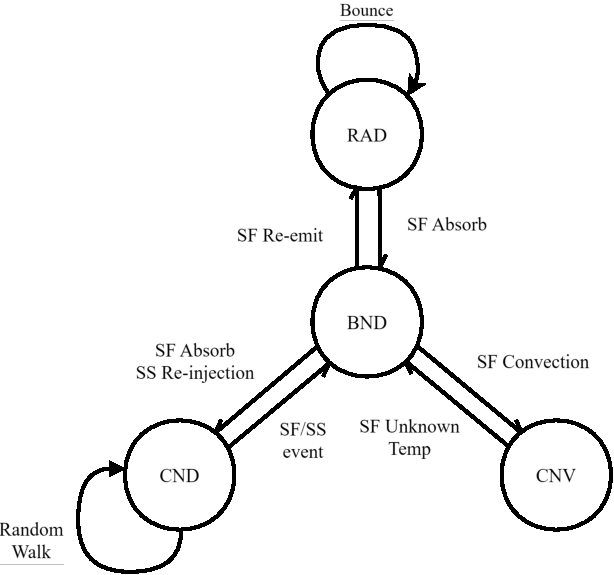
\includegraphics[width=0.6\textwidth]{Figures/Coupled_Path_Meta_SM/CPML.pdf}
  \bicaption{耦合路径的四模态转换关系图}{Module-level transition graph of coupled heat transport path}
  \label{fig:coupled_path_meta}

  \small
  四个节点分别对应辐射（RAD）、界面（BND）、传导（CND）、对流（CNV）模块，
  有向边标注触发模态转换的物理事件。路径在同一路径空间中按概率在各模态间切换，
  第三章将进一步展开每个模块内部的有限状态机设计。
\end{figure}

框架中的路径由三类路径段按物理规律拼接而成：
\begin{itemize}
    \item 辐射段（RAD）：光子在透明介质中沿直线传播，方向不变、强度不衰减（漫射灰体简化下），路径步进由几何相交查询驱动，直至命中固体表面触发界面事件（BND）。
    \item 传导段（CND）：热量在固体内通过布朗随机游走（Brownian motion）传输。更一般地，考虑含体积热源的稳态传导方程（Poisson 方程）$k\nabla^2\theta + q = 0$ 在域 $\Omega$ 上的 Dirichlet 问题 $\theta|_{\partial\Omega} = g$，Feynman-Kac 公式\cite{kacRandomWalkTheory1947}将其解表示为布朗路径的期望：
    \begin{equation}
        \theta(\mathbf{x}) = E_{\mathbf{x}}\!\left[g(B_\tau) + \int_0^\tau \frac{q(B_s)}{2k}\,\mathrm{d}s\right]
        \label{eq:feynman_kac}
    \end{equation}
    其中 $B_t$ 为从 $\mathbf{x}$ 出发的标准布朗运动（生成元 $\frac{1}{2}\nabla^2$），$\tau = \inf\{t > 0 : B_t \in \partial\Omega\}$ 为首次到达边界的停止时间。右端第一项 $g(B_\tau)$ 为路径终止于边界时读取的边界温度；第二项为路径沿途累加的体积热源贡献——每一步随机游走处的功率密度 $q$ 通过 Green 函数系数转化为温度增量。当 $q=0$ 时退化为经典 Kac 公式 $\theta(\mathbf{x}) = E[g(B_\tau)]$\cite{treganCouplingRadiativeConductive2023}。类似地，界面处指定的表面热流密度（Neumann 条件）也在路径经过时以对应系数累加为温度贡献。Feynman-Kac 公式使传导问题的蒙特卡洛求解与辐射路径追踪在形式上统一：两者都沿随机路径追踪，沿途累加源项，终止于已知边界。该公式的成立依赖传导方程的线性性——传导方程的 Green 函数恰好是布朗运动的转移概率密度。这一线性性要求是 2.1.4 中 Constraint 5（$h_R$ 线性化）的数学根源：辐射项的 $\sigma T^4$ 非线性在线性化后才能纳入随机游走框架。上述公式是稳态特例；对于瞬态传导方程 $\partial\theta_S / \partial t = \alpha \nabla^2 \theta_S$，Bati 等人\cite{batiCouplingConductionConvection2023}将有限差分空间离散后的扩散方程改写为指数分布的时间回退（backward time jump）形式：每一步 $\delta$-球面游走采样指数分布的回退时长 $T_{b,\text{cond}} \sim \mathrm{Exp}(\tau_\text{cond})$（均值 $\tau_\text{cond} = \rho c_p \tilde{\delta}^2 / (6k)$，即 $\delta$-球面尺度上的传导弛豫时间），将路径时间从观测时刻 $t$ 向初始时刻 $t_I$ 回退。若 $t - T_{b,\text{cond}} \leq t_I$，路径终止并返回初始温度场 $\theta_S(\mathbf{x}, t_I)$；否则继续游走。辐射在透明介质中以光速传播，渡越时间相对于传导弛豫时间可忽略，因此辐射段（RAD）不涉及时间回退。
    \item 对流段（CNV）：路径到达施加对流边界条件的固-流界面时，以 $P_\text{conv}$ 概率选择对流分支。该段同样携带时间回退机制：采样指数分布的回退时长 $T_{b,\text{conv}} \sim \mathrm{Exp}(\tau_\text{conv})$（均值 $\tau_\text{conv} = \rho c V / (h\mathcal{S})$，为流体腔的对流弛豫时间），若回退至 $t \leq t_I$ 则返回初始流体温度 $\theta_F(t_I)$；否则在流体腔的固-流界面上按对流系数 $h$ 加权采样一个位置，取该处固体侧温度作为流体温度的无偏估计，路径随后从该采样位置继续进入下一轮界面分叉。
\end{itemize}

三类路径段在固-流界面处（BND 过程）以随机方式发生模态转换：路径按界面物理参数决定的概率随机选择进入 CND（传导游走）、CNV（对流采样）或 RAD（辐射再发射）模块（详见下文界面耦合方程）。Bati 等人框架的一个显著特性是路径权重恒为 $W = 1$（单位权重）\cite{batiCouplingConductionConvection2023}：在每个事件点，路径以物理导出的精确概率选择分支——三模态概率来自能量守恒、俄罗斯轮盘赌吸收率 $\varepsilon$ 精确等于物理吸收率、余弦加权方向采样与辐射通量核 $\cos\theta / \pi$ 精确匹配——采样概率与被积函数权重精确相消，全程无需额外的权重修正因子。

在该框架下，路径终止于且仅终止于以下两类条件之一：(1) 路径到达温度已知的空间位置（imposed temperature），包括 Dirichlet 恒温边界和辐射路径逃逸至场景外部时读取的环境温度 $\theta_\text{env}$；(2) 传导段或对流段的时间回退累计达到初始时刻 $t_I$，路径读取初始温度场 $\theta_S(\mathbf{x}, t_I)$ 或初始流体温度 $\theta_F(t_I)$。第 (2) 类终止条件反映了传导与对流过程的瞬态弛豫特性：路径的时间坐标从观测时刻向过去回退，每经历一步传导游走或对流采样都消耗一段随机时长（指数分布，均值分别为 $\tau_\text{cond}$ 和 $\tau_\text{conv}$），当累计回退超过 $t - t_I$ 时路径即终止于初始条件。辐射段不回退时间（光速渡越可忽略），因此辐射不产生此类终止。对于稳态问题（$t - t_I \to \infty$），所有路径最终都终止于条件 (1)。

对任意空间点 $\mathbf{x}$ 在观测时刻 $t$ 的温度，从 $\mathbf{x}$ 出发独立发射 $N$ 条路径，每条路径经历若干次模态转换后终止于上述条件之一，记第 $i$ 条路径的终止温度为 $\theta_\text{term}^{(i)}$。由于单位权重特性，$\theta_\text{term}^{(i)}$ 本身即为 $\theta(\mathbf{x}, t)$ 的无偏估计，$N$ 条路径的估计量取算术均值：
\begin{equation}
    \hat{\theta}(\mathbf{x}) = \frac{1}{N}\sum_{i=1}^{N} \theta_\text{term}^{(i)}
    \label{eq:estimator}
\end{equation}
其中 $\hat{\theta}(\mathbf{x})$ 为点 $\mathbf{x}$ 处温度的蒙特卡洛估计值，$N$ 为独立采样路径数，$\theta_\text{term}^{(i)}$ 为第 $i$ 条路径的返回值——包含路径终止于已知边界时读取的温度（Dirichlet 边界温度、环境温度或初始温度场），以及路径沿途经过的体积热源和表面热流密度对温度的累加贡献（式\,\ref{eq:feynman_kac} 中的积分项）。该公式是等权算术均值而非加权和——这正是单位权重特性的直接体现：若路径携带非单位权重 $W^{(i)} \neq 1$，则估计量应为 $\hat{\theta} = \sum W^{(i)}\theta_\text{term}^{(i)} / \sum W^{(i)}$。估计量的物理含义取决于起始模态：从探测器像素出发的路径估计辐射温度（经 $L = \sigma\theta^4/\pi$ 变换为辐射亮度），从固体内部点出发的路径估计该点在时刻 $t$ 的温度。

\textbf{固-流界面（S-F）耦合}。在固-流界面处，固体侧传导热通量等于流体侧对流通量与辐射通量之和。Bati 等人通过有限差分线性化将此能量守恒条件改写为概率期望形式，使界面温度可表示为三种传输模态贡献的概率加权和\cite{batiCouplingConductionConvection2023}：
\begin{equation}
  \theta_S(\mathbf{x}) = P_\text{cond}\,\theta_S(\mathbf{x}-\delta\hat{n})
  + P_\text{conv}\,\theta_F
  + P_\text{rad}\int_{2\pi}\theta_R\,\frac{\boldsymbol{\omega}\cdot\hat{n}}{\pi}\,\mathrm{d}\boldsymbol{\omega}
  \label{eq:interface_temp}
\end{equation}
其中 $\theta_S(\mathbf{x}-\delta\hat{n})$ 为沿法线向固体内部偏移 $\delta$ 处的温度（传导贡献），$\theta_F$ 为对流流体温度，$\theta_R$ 为辐射温度。三个概率由界面物理参数决定：
\begin{equation}
  P_\text{cond} = \frac{k/\delta}{k/\delta + h + h_R}, \quad
  P_\text{conv} = \frac{h}{k/\delta + h + h_R}, \quad
  P_\text{rad} = \frac{h_R}{k/\delta + h + h_R}
  \label{eq:interface_probs}
\end{equation}
其中 $k$ 为固体导热系数，$h$ 为对流换热系数，$h_R = 4\sigma\varepsilon\theta_\text{ref}^3$ 为辐射线性化等效换热系数。辐射项中的 $T^4$ 非线性使联合边界条件无法直接改写为线性概率形式。Bati 等人\cite{batiCouplingConductionConvection2023}采用线性化处理：在参考温度 $\theta_\text{ref}$ 附近对 $\sigma T^4$ 截取一阶 Taylor 展开，由此定义 $h_R = 4\sigma\varepsilon\theta_\text{ref}^3$，将辐射通量近似为与 $T$ 的线性关系，使三模态概率可在给定 $\theta_\text{ref}$ 下预先计算且恰好满足 $P_\text{cond} + P_\text{conv} + P_\text{rad} = 1$。$\theta_\text{ref}$ 的准确度直接影响线性化误差——当实际温度与 $\theta_\text{ref}$ 偏差较大时，$h_R$ 偏离真值，导致概率失准。为此，Bati 等人在论文展望部分引入 Null-collision 接受/拒绝机制（2.2.3）：以 $h_R$ 上界计算概率，采样后根据实际温度决定接受或拒绝，保证估计量无偏。路径在界面处按上述概率随机选择进入 CND（传导游走）、CNV（对流采样）或 RAD（辐射再发射）模块，实现了三种传热模态在同一路径空间中的概率耦合。

当路径以 $P_\text{conv}$ 概率选择对流分支时，需估计流体温度 $\theta_F$。该框架将 $\theta_F$ 表示为流体腔封闭面上固-流界面温度的加权期望\cite{batiCouplingConductionConvection2023}：
\begin{equation}
  \theta_F = E\bigl[\theta_S(X_S)\bigr], \quad X_S \sim p_h(\mathbf{x}) \propto h(\mathbf{x})
  \label{eq:fluid_temp}
\end{equation}
即在流体腔的固-流界面上按对流系数 $h$ 分布采样一个位置 $X_S$，取该处固体侧温度作为 $\theta_F$ 的无偏估计。路径随后继续从 $X_S$ 处的界面进入下一轮耦合分叉。

\textbf{固-固界面（S-S）耦合}。当传导游走路径到达两个相邻固体的接触面时，物理方程为传导通量连续条件\cite{batiCouplingConductionConvection2023}：
\begin{equation}
  \theta_S(\mathbf{x}) = P_{\text{cond},1}\,\theta_S(\mathbf{x}-\delta_1\hat{n})
  + P_{\text{cond},2}\,\theta_S(\mathbf{x}+\delta_2\hat{n})
  \label{eq:ss_interface}
\end{equation}
其中 $P_{\text{cond},1} = (k_1/\delta_1)/(k_1/\delta_1 + k_2/\delta_2)$，$P_{\text{cond},2} = 1 - P_{\text{cond},1}$。路径以此概率选择注入固体 1 或固体 2 侧的 $\delta$ 偏移处，继续传导游走。固-固界面不涉及辐射和对流模态，分叉结构仅为二元导热概率选择。


\subsection{递归路径追踪求解器}
%% 写作思路：
%%   - 以 Bati Appendix B 的 4 个互递归算法为线索，取代代码结构线索。
%%   - 4 个子例程（BND/RAD/CND/CNV），每个返回温度值。
%%   - 尾递归、无权重累乘、终止于 Dirichlet 边界或环境温度。
%% [引用需求] \cite{batiCouplingConductionConvection2023}

基于上述耦合路径追踪框架，Bati 等人\cite{batiCouplingConductionConvection2023}给出了由四个互递归子例程构成的递归求解器（附录 B, Algorithms 1--4），每个子例程对应一种传热模态或界面分发过程，返回值均为温度。对任意探测点 $\mathbf{x}$，温度估计量由 $N$ 条独立路径的返回值取均值得到：$\hat{\theta}(\mathbf{x}) = \frac{1}{N}\sum_{i=1}^{N}\theta_\text{term}^{(i)}$。

四个子例程的物理含义与递归关系如下。界面分发（BND，算法\,\ref{alg:bnd}）是耦合的核心枢纽：路径到达固体界面时，首先识别界面类型（固-流或固-固），然后按物理概率将路径分发至相应的传热模态。辐射子路径（RAD，算法\,\ref{alg:rad}）沿当前方向执行光线追踪，循环处理反射/吸收事件直至被表面吸收或逃逸至环境。传导子路径（CND，算法\,\ref{alg:cnd}）在固体内执行 $\delta$-球面随机游走，每步沿随机方向前进并回退时间，直至到达初始时刻或固体边界。对流子路径（CNV，算法\,\ref{alg:cnv}）采样对流时间常数并回退时间，到达初始时刻返回流体温度，否则在固-流界面上按对流系数加权采样位置后重新进入界面分发。

\begin{algorithm}
\caption{界面分发子例程（BND）}
\label{alg:bnd}
\begin{algorithmic}[1]
\REQUIRE 界面位置 $\mathbf{x}$，当前时间 $t$
\ENSURE 温度 $\theta$
\IF{$\mathbf{x}$ 在固-固界面（S-S）}
  \STATE 计算 $P_{\text{cond},1},\,P_{\text{cond},2}$（基于两侧 $k/\delta$，式\,\eqref{eq:ss_interface}）
  \STATE 随机选择侧 $i$ $\rightarrow$ \textbf{return} \textsc{ConductiveSubpath}($\mathbf{x} + \delta_i\hat{n}_i,\,t$)
\ELSIF{$\mathbf{x}$ 在固-流界面（S-F）}
  \STATE 计算 $P_\text{conv},\,P_\text{cond},\,P_\text{rad}$（式\,\eqref{eq:interface_probs}）
  \STATE $r \leftarrow \mathrm{uniform}[0,1)$
  \IF{$r < P_\text{conv}$}
    \STATE \textbf{return} \textsc{ConvectiveSubpath}($t$)
  \ELSIF{$r < P_\text{conv} + P_\text{cond}$}
    \STATE \textbf{return} \textsc{ConductiveSubpath}($\mathbf{x} - \delta\hat{n},\,t$)
  \ELSE
    \STATE $\hat{\boldsymbol{\omega}} \leftarrow$ 余弦加权半球采样
    \STATE \textbf{return} \textsc{RadiativeSubpath}($\mathbf{x},\,\hat{\boldsymbol{\omega}}$)
  \ENDIF
\ENDIF
\end{algorithmic}
\end{algorithm}

\begin{algorithm}
\caption{辐射子路径（RAD）}
\label{alg:rad}
\begin{algorithmic}[1]
\REQUIRE 位置 $\mathbf{x}$，方向 $\hat{\boldsymbol{\omega}}$
\ENSURE 温度 $\theta$
\LOOP
  \STATE $s \leftarrow$ 沿 $\hat{\boldsymbol{\omega}}$ 光线追踪求最近交点
  \IF{$s = \infty$（未命中）}
    \STATE \textbf{return} $\theta_\mathrm{env}$ \COMMENT{环境温度}
  \ENDIF
  \STATE $\mathbf{x} \leftarrow \mathbf{x} + s\hat{\boldsymbol{\omega}}$
  \IF{$\mathrm{uniform}[0,1) < \varepsilon(\mathbf{x})$}
    \STATE \textbf{return} \textsc{BoundaryDispatch}($\mathbf{x},\,t$) \COMMENT{吸收 $\rightarrow$ 界面分发}
  \ELSE
    \STATE $\hat{\boldsymbol{\omega}} \leftarrow$ 按表面 BRDF 采样新方向 \COMMENT{反射 $\rightarrow$ 继续循环}
  \ENDIF
\ENDLOOP
\end{algorithmic}
\end{algorithm}

\begin{algorithm}
\caption{传导子路径（CND）}
\label{alg:cnd}
\begin{algorithmic}[1]
\REQUIRE 位置 $\mathbf{x}$，时间 $t$
\ENSURE 温度 $\theta$
\LOOP
  \STATE $\hat{\boldsymbol{\omega}} \leftarrow$ 各向同性方向采样
  \STATE $\tilde{\delta} \leftarrow \min(\delta,\,\text{沿}\pm\hat{\boldsymbol{\omega}}\text{到最近边界距离})$
  \STATE $\Delta t \leftarrow$ 采样指数分布（均值 $\rho c_p \tilde{\delta}^2 / (6k)$）
  \STATE $t \leftarrow t - \Delta t$ \COMMENT{时间回退}
  \IF{$t \leq t_I$}
    \STATE \textbf{return} $\theta_S(\mathbf{x},\,t_I)$ \COMMENT{到达初始时刻}
  \ENDIF
  \STATE $\mathbf{x} \leftarrow \mathbf{x} + \tilde{\delta}\hat{\boldsymbol{\omega}}$
  \IF{$\mathbf{x}$ 在边界上}
    \STATE \textbf{return} \textsc{BoundaryDispatch}($\mathbf{x},\,t$) \COMMENT{到达界面 $\rightarrow$ 分发}
  \ENDIF
\ENDLOOP
\end{algorithmic}
\end{algorithm}

\begin{algorithm}
\caption{对流子路径（CNV）}
\label{alg:cnv}
\begin{algorithmic}[1]
\REQUIRE 时间 $t$
\ENSURE 温度 $\theta$
\STATE $\Delta t \leftarrow$ 采样指数分布（均值 $\tau_\text{conv}$）
\STATE $t \leftarrow t - \Delta t$ \COMMENT{时间回退}
\IF{$t \leq t_I$}
  \STATE \textbf{return} $\theta_F(t_I)$ \COMMENT{到达初始时刻 $\rightarrow$ 流体温度}
\ENDIF
\STATE $\mathbf{x}_S \leftarrow$ 在固-流界面上按 $h(\mathbf{x})$ 加权采样位置
\STATE \textbf{return} \textsc{BoundaryDispatch}($\mathbf{x}_S,\,t$) \COMMENT{采样位置 $\rightarrow$ 界面分发}
\end{algorithmic}
\end{algorithm}

上述四个子例程构成互递归调用图：BND 根据界面类型和物理概率选择模态分支，各模态子例程在路径到达新界面时回调 BND，形成递归展开。路径展开以深度优先方式进行，每次递归调用返回温度值，不涉及权重累乘——单位权重特性（\ref{sec:coupled_framework}）保证每次模态分叉的采样概率与物理贡献精确相消。路径终止于两种条件之一：(1) 到达已知温度的 Dirichlet 边界或环境温度；(2) 时间回退至初始时刻 $t_I$。

此递归结构在正确性上完整复现了 \ref{sec:coupled_framework} 的耦合路径追踪框架理论。然而，其将路径状态隐式绑定于函数调用栈的实现特性——四个子例程的互递归展开导致路径的全部中间状态分散于多层栈帧中，既不可序列化也不可中断恢复——构成了面向并行化改造时的深层结构性障碍，下一小节将从四个递推角度展开分析。

\subsection{递归求解框架的局限性分析}
\label{sec:dfs_limitations}

2.2.5 的递归求解器通过同步阻塞的几何查询调用驱动路径状态机前进：每次查询提交后函数原地等待结果返回，然后依据结果执行后续物理计算。对该求解器控制流的完整分析表明，一条路径从发射到终止典型需经历 50--200 次同步几何查询，最坏情况可达数千次，且每次均以宽度为 1 的串行方式执行。虽然不同像素间的路径在统计层面完全独立，但递归求解器在架构层面将这种并行潜力完全放弃。以下从四个相互递推的角度分析其结构性障碍，四者均源于同一根因：路径状态与执行控制流的隐式耦合。

\subsubsection{障碍 A：调度粒度过大}

递归求解器将路径完整求解过程封装为一次连续的函数调用链，涵盖 RAD、BND、CND、CNV 全部物理逻辑。若将该调用链直接映射到单一 GPU kernel（即 MegaKernel 方案），则 kernel 体积极大，寄存器需求量极高，且递归深度受 GPU 栈空间严格限制——GPU 单 SM 的 warp 占用率远低于理论峰值。即便忽略栈深度限制，同一 warp 内各路径所处物理阶段不同（部分执行 RAD 弹射，部分处于 CND 游走，部分进入 BND 概率分叉），指令路径严重分叉，SIMT 执行效率大幅下降。

\subsubsection{障碍 B：路径状态不可持久化}

更深层的障碍在于递归求解器的状态保存方式。路径的全部中间状态（位置、方向、权重、路径深度、随机数状态等）分散在多层调用栈帧的局部变量中，是程序控制流的副产物而非独立数据对象。这些信息无法在函数调用途中以完整快照形式导出：函数若不等待查询结果便无法正常返回，而强行返回则栈帧释放、中间状态不可恢复地丢失。因此路径执行不具有中断、挂起与恢复的能力。

\subsubsection{障碍 C：几何查询请求无法批量积累}

批量化要求在同一时刻积累多条路径的查询请求后统一提交。该要求以两个条件为前提：(1) 多条路径能同时推进到各自的查询节点；(2) 存在统一的调度视角收集这些请求。递归求解器的同步阻塞结构使两个条件均不成立——第一条路径的查询调用占用控制流直至结果返回，其他路径无法推进；即使多线程化，各线程各自独立阻塞，系统不存在能观察全部等待路径的全局调度节点。几何查询提交宽度恒为 1，无法触及 SIMD packet 批量接口，更无法将请求卸载至 GPU 硬件光追管线。

\subsubsection{障碍 D：复合物理分支无法拆分调度}

路径在 BND 界面事件中产生复合物理分支：以概率 $\varepsilon$ 吸收转入传导/对流，以 $1-\varepsilon$ 漫反射继续辐射传播；null-collision 循环内还可能递归生成子路径树以评估辐射贡献。这些分支以嵌套函数调用形式展开，分叉发生在运行时且依赖查询结果，不同路径的分支选择完全异步——若将不同分支处的路径混合调度，无法统一选定推进方向，形成闭环依赖。

\subsubsection{局限性总结}

四大障碍层层递推：路径状态绑定于调用栈（障碍 B）导致不可挂起，使查询请求无法跨路径积累（障碍 C）；调度粒度锁定在完整路径生命周期（障碍 A），叠加物理分支无法拆分（障碍 D），使递归求解架构下任何批量化策略均不可行。要实现批量化，必须将路径状态从调用栈中显式提取为独立的可序列化数据结构，将状态推进与几何查询执行解耦为两个独立阶段——这正是 2.3 Wavefront 执行模型的设计出发点，也是第三章 Wavefront 求解器实现的直接依据。

\section{Wavefront 执行模型}
%% [篇幅需求] 约1000字，重在阐明批量化障碍与解耦范式，无需深入第三章的实现细节。
%% [写作总思路]
%%   从 DFS 固有的同步耦合结构出发（2.3.1），引出 Wavefront 解耦范式（2.3.2），
%%   最后分析对耦合热输运的适用性并如实交代解耦引入的 Cache 代价（2.3.3）。
%%   不以 GPU Warp 发散为主逻辑链，而以"DFS 1-宽度同步结构无法积累批量查询"为核心动机。

\subsection{从递归求解框架的障碍到批量化需求}
%% 简要衔接 2.2.6 与 Wavefront 范式

2.2.6 的四大障碍分析揭示了递归求解架构无法实现批量几何查询的根本结构性原因：路径状态与执行控制流的隐式耦合。其中，障碍 B（路径状态不可持久化）和障碍 C（查询请求无法批量积累）指向最直接的解法方向——将状态推进与查询执行从同一控制流中解耦为两个独立阶段。这正是 Wavefront 执行范式的核心思想。

\subsection{Wavefront范式：解耦状态推进与查询执行}
%% 写作思路：
%%   - 核心思想（硬件无关）：路径维护持久化状态结构体，CPU 推进路径状态机；
%%     当路径抵达需要几何查询的节点时，将请求写入挂起队列（pending queue），
%%     路径进入 PENDING 状态挂起；CPU 继续推进其他路径；
%%     积累完毕后统一提交给几何查询后端；结果返回后路径从 PENDING 恢复继续推进。
%%   - Laine et al. 2013 起源（一句带过）：原始动机是解决 GPU Megakernel 的 Warp 发散
%%     和寄存器压力问题，但解耦结构的价值独立于具体硬件。
%%   - 本文三类 PENDING：RT（射线最近命中）、ENC（封闭腔体归属查询）、
%%     CP（最近面投影），三类由耦合热输运物理过程决定；Wavefront 使其自然积累
%%     为批量请求，后端如何高效执行是独立设计问题（第四章）。
%% [图表需求] Wavefront 双阶段循环示意（CPU 推进阶段 → pending queue → GPU 执行阶段 → 恢复）
%% [引用需求] \cite{laineMegakernelsConsideredHarmful2013}

Wavefront 范式通过引入持久化路径状态与挂起队列机制，在架构层面将状态推进与查询执行分离为两个独立的执行阶段。每条路径拥有一个长期驻留于内存的状态结构体，记录其当前位置、方向、累积权重、命中信息及物理状态标识。CPU 推进阶段遍历所有路径，逐条将其在状态机中向前推进；当某条路径到达需要几何查询的节点时，CPU 将该查询请求写入对应的挂起队列（pending queue），路径进入 PENDING 状态等待，CPU 立即继续处理下一条路径，而不阻塞等待。待本轮推进完成，所有进入 PENDING 的路径已自然积累为一批同类查询请求，统一提交至几何查询后端执行。后端执行阶段完成批量查询后，将结果写回各路径的状态结构体，路径从 PENDING 状态恢复，等待下一轮 CPU 推进阶段继续向前。上述两阶段交替循环，直至所有路径终止采样。

这一范式最早由 Laine 等人在 GPU 路径追踪场景中以"Wavefront"之名提出，彼时的原始动机是解决 Megakernel 架构下因路径状态异质而导致的 Warp 发散与寄存器压力问题。然而，解耦结构的核心价值——将状态推进与查询执行分离，使批量查询自然涌现——独立于 GPU 硬件存在：在 GPU 上，挂起路径对应 kernel 间的全局显存队列；在 CPU 多线程实现中，挂起路径则对应线程池共享的内存数组，同样可获得批量积累的效果。

在耦合热输运求解中，几何查询并非单一类型，而是按用途分为三类，各自对应不同的查询语义与 GPU 实现管线：RT 查询（ray tracing，沿路径方向找到第一个几何交点，驱动所有涉及直接射线求交的物理过程）、ENC 查询（enclosure，给定空间点判断其所属封闭腔体，用于 BND 界面事件中的腔体归属判断）、CP 查询（closest point，给定空间点求场景表面最近点，仅用于传导段 CND 中 Walk-on-Spheres 游走路径的步长计算）。路径推进至需要上述任一查询时即进入对应类型的 PENDING 状态，三类挂起队列在每轮推进后各自积累为一组同类批量请求统一提交。三类查询的语义与分类由耦合热输运的物理过程决定，而非由特定后端驱动；Wavefront 框架使这些请求自然地以批量形式呈现给查询后端，后端如何高效处理这些批量请求则是独立于 Wavefront 范式之外的工程设计问题。

\subsection{适用性分析与解耦引入的 Cache 代价}
%% 写作思路：
%%   - 适用性：四状态路径与渲染路径同构，CPU 线性遍历路径数组自然积累三类 PENDING，
%%     无需按状态排序分桶（排序引入数据重排开销，路径数有限时收益不明显）。
%%   - Cache 代价：DFS 对照组仅维护单条路径的栈上状态（L1 完全覆盖）；
%%     Wavefront 需同时维护 N 条路径的持久化结构体（工作集远超缓存容量），
%%     遍历时对每条路径的随机访问几乎均为 cache miss，是本实现头号性能瓶颈。
%%   - 此代价与架构绑定，是实现解耦的必要代价；优化方向（SoA 布局等）留给第三章。
%% [引用需求] \cite{laineMegakernelsConsideredHarmful2013}

耦合热输运路径在 RAD/BND/CND/CNV 四类状态间按物理规律切换，与图形渲染路径的状态机结构高度同构，Wavefront 范式对本问题天然适用。在具体实现中，CPU 推进阶段只需按顺序线性遍历路径数组，逐条将各路径推进至下一个 PENDING 节点，无需预先对路径按状态排序分桶——分桶操作涉及额外的数据重排开销，且在路径总数有限的工程场景中收益不明显；三类 PENDING 挂起队列中的查询请求在遍历过程中自然积累，作为本轮推进的副产品直接送达后端。

然而，解耦带来的批量查询能力是以一项新的 Cache 代价为前提的，该代价在递归求解器对照组中完全不存在。在递归求解器框架中，同一时刻只有一条路径处于活跃状态，其全部状态数据（位置、方向、权重、命中信息等）驻留于 CPU 调用栈上，体量极小，可完全驻留于 L1 缓存，访问延迟可忽略不计。而 Wavefront 实现需要同时将 $N$ 条路径的状态结构体长期保存于主存——$N$ 越大，积累的批量查询规模越大，查询后端可从中获取更高的并行执行效率；但 $N$ 个结构体构成的内存工作集随 $N$ 的增大迅速超出 CPU 末级缓存（LLC）的容量。CPU 推进阶段线性遍历路径数组时，对每条路径状态结构体的访问在缓存中几乎均无命中，频繁触发 cache miss 与主存访问，产生显著的访问延迟。这一 Cache 压力是本实现相对对照组引入的独有性能瓶颈，也是驱动第三章中状态结构体布局优化（结构体数组 AoS 与数组结构体 SoA 的权衡）等设计决策的直接原因。

综上，Wavefront 范式的核心贡献是将状态推进与查询执行解耦，使大批量几何查询从架构层面成为可能；其代价是持久化路径状态数组带来的 Cache 压力。正确认识这一权衡，是理解本文混合架构设计选择和第三章性能分析的基础。

\section{光线追踪与几何查询加速技术}
%% [篇幅需求] 约2000字，从算法原理到工程实现，为第四章 OptiX 后端的设计决策提供理论依据。
%% [写作总思路]
%%   先讲光线-几何求交的基础算法（2.4.1），再介绍使求交加速几个数量级的 BVH 加速结构（2.4.2），
%%   然后分别介绍 CPU（2.4.3）和 GPU（2.4.4）两条工程实现路线，
%%   最后扩展到本文实际需要的三类几何查询（2.4.5），为第四章的后端管线设计直接铺垫。

\subsection{光线-几何求交算法}
%% [写作思路（已修订）]
%%   - 问题定义：光线参数方程，求最近交点 $(t^*, u^*, v^*)$。
%%   - Möller-Trumbore（MT）算法：Cramer 法则直接求解，简洁高效，是概念参考实现。
%%     但 MT 不满足水密性：共享棱边/顶点处两相邻三角形独立计算，浮点舍入可能导致
%%     双重漏判（穿透缝隙）或双重命中（虚假散射）。
%%   - 为什么需要水密性：封闭网格表示真实物理固体边界；穿透缝隙令蒙特卡洛粒子泄入
%%     错误腔体，破坏腔体归属和权重贡献；低仰角红外成像场景（掠角观测）对此最为敏感。
%%   - WBW（Wald-Benthin-Woop）水密算法：将求交变换到射线对齐坐标系，以棱函数的
%%     符号一致性判别消除共享棱/顶点歧义，保证相邻三角形各自对共享边界唯一所有权。
%%   - WBW 是工业实施标准：Embree 默认求交内核（配合 SIMD 批量）；
%%     NVIDIA RT Core 固定功能求交电路的硬件设计基础。
%% [公式需求] 光线参数方程、MT Cramer 解、WBW 棱函数
%% [引用需求] \cite{MollerTrumbore1997,WaldBenthinWoop2013}

光线追踪的基本操作是给定一条射线，在三角形网格场景中快速求出最近交点。射线以参数方程定义：
\begin{equation}
    \mathbf{r}(t) = \mathbf{o} + t\hat{\mathbf{d}}, \quad t \in [t_{\min},\, t_{\max}]
    \label{eq:ray}
\end{equation}
其中 $\mathbf{o}$ 为原点，$\hat{\mathbf{d}}$ 为归一化方向，$t_{\min} > 0$ 用于排除起点处的自相交，$t_{\max}$ 为远截面截断。对顶点坐标为 $\mathbf{p}_0, \mathbf{p}_1, \mathbf{p}_2$ 的三角形，命中条件等价于求解线性方程组：
\begin{equation}
    \mathbf{o} + t\hat{\mathbf{d}}
    = (1 - u - v)\,\mathbf{p}_0 + u\,\mathbf{p}_1 + v\,\mathbf{p}_2,
    \quad u \geq 0,\; v \geq 0,\; u + v \leq 1
    \label{eq:mt_system}
\end{equation}
令 $\mathbf{e}_1 = \mathbf{p}_1 - \mathbf{p}_0$，$\mathbf{e}_2 = \mathbf{p}_2 - \mathbf{p}_0$，$\mathbf{s} = \mathbf{o} - \mathbf{p}_0$，Cramer 法则直接给出 Möller-Trumbore（MT）算法：
\begin{equation}
\begin{pmatrix} t \\ u \\ v \end{pmatrix}
= \frac{1}{(\hat{\mathbf{d}} \times \mathbf{e}_2) \cdot \mathbf{e}_1}
  \begin{pmatrix}
    (\mathbf{s} \times \mathbf{e}_1) \cdot \mathbf{e}_2 \\
    (\hat{\mathbf{d}} \times \mathbf{e}_2) \cdot \mathbf{s} \\
    (\mathbf{s} \times \mathbf{e}_1) \cdot \hat{\mathbf{d}}
  \end{pmatrix}
\label{eq:moller_trumbore}
\end{equation}
MT 算法结构极为简洁——仅需 1 次叉积与 3 次点积，无需预存三角形法向量，长期作为概念参考实现广泛使用。然而，MT 算法不满足水密性（watertightness）的工程要求。

射线求交算法的水密性需求源自以下数值问题：在以三角形网格表示的封闭固体中，相邻三角形共享棱边和顶点。当射线以极小入射角掠过共享棱边时，两个相邻三角形各自独立地以浮点运算计算重心坐标，判定条件 $u \geq 0,\, v \geq 0,\, u+v \leq 1$ 的数值结果均落在零附近；不同量级的中间舍入误差可引发两类相反的不一致：若两个三角形均错误地返回"不命中"，则共享棱边处产生数值裂缝，射线得以穿透封闭表面；若两个三角形均返回"命中"，则同一边界点被重复计数，产生虚假的双重散射事件。

在蒙特卡洛耦合热输运求解中，上述两类失效均直接破坏物理正确性。穿透失效使传导段布朗游走粒子越过物理边界进入错误腔体：一旦腔体归属（\texttt{enc\_id}）出错，粒子此后所读取的材质参数、发射率及对流换热系数全部来自错误腔体，对应样本的完整权重贡献均为系统性偏差而非统计噪声，无法通过增加样本量消除。双重命中失效使辐射路径在掠角方向上被提前终止或双倍统计，引入方向相关的偏差。两类误差在低仰角红外成像（掠角观测）场景中最为集中——极小入射角正是最频繁触发共享棱边临界情形的几何配置，而低仰角观测又是红外探测的重要应用场景。MT 算法对掠棱情形的判定结果完全依赖各三角形各自的浮点舍入，无法为相邻三角形之间建立任何一致性保证，不能满足物理仿真对几何边界一致性的严格要求。

为了满足水密性要求，Wald、Benthin 与 Woop 提出将求交问题变换到射线对齐坐标系（ray-aligned frame）中处理，以彻底消除共享棱边/顶点处的分类歧义\cite{woopWatertightRayTriangle2013}。算法分离线预处理与在线查询两个阶段：

\textit{预处理阶段（逐三角形，离线完成）}：对每个三角形预计算一个 $3\times 4$ 仿射变换矩阵 $M$，将世界坐标映射到以查询射线方向为 $+z$ 轴的局部坐标系——三角形在此坐标系的 $z=1$ 截面退化为标准单位三角形，三个顶点变换后的局部坐标分量记为 $(x_i, y_i, z_i)$，$i=0,1,2$。

\textit{查询阶段（逐射线，在线执行）}：以 $M$ 将光线原点变换至局部坐标后，命中判定转化为三个有符号棱函数（edge function）的符号一致性检验：
\begin{equation}
    e_0 = x_1 y_2 - x_2 y_1,\quad
    e_1 = x_2 y_0 - x_0 y_2,\quad
    e_2 = x_0 y_1 - x_1 y_0
    \label{eq:WBW_edge}
\end{equation}
当且仅当 $e_0, e_1, e_2$ 同号（均 $\geq 0$ 或均 $\leq 0$）时判定命中，命中参数为 $t = (e_0 z_0 + e_1 z_1 + e_2 z_2)/(e_0 + e_1 + e_2)$。水密性的关键在于：将 $e_i = 0$（射线恰好掠过该棱边）归入正方向一侧——即 $0$ 满足"$\geq 0$"——保证共享此棱边的相邻两三角形中恰好一个声明对边界点的所有权，另一个三角形对应的棱函数值与之互为相反符号，被排除在命中判定之外，从而在数学上彻底消除双重命中与双重漏判的可能性。

WBW 算法是现代高性能光追软件与图形硬件的实施标准。Intel Embree 将 WBW 求交内核与 SIMD 指令相结合，通过射线包（ray packet）模式同时对 4/8/16 条射线执行批量坐标变换与符号判别，在保证水密性的同时充分利用向量并行能力。NVIDIA 自 Turing 架构起引入的 RT Core 硬件固定功能单元，其内部求交电路以 WBW 坐标变换与棱函数符号一致性逻辑为核心，在晶体管层面实现了每时钟周期完成多组射线—三角形水密求交的全流水线设计。正是这一从算法到硬件的统一实施路线，确保了在任意复杂封闭网格场景中，几何表面对光线路径和随机游走粒子始终是严格不可穿透的。

\subsection{层次包围体加速结构}
%% 写作思路：
%%   - 暴力检测的复杂度：$O(N)$（$N$ 为三角形数），大规模场景（百万面片）不可接受。
%%   - BVH 的核心思想：将场景三角形组织为二叉树，每个节点包含其子树所有三角形的
%%     轴对齐包围盒（AABB）；光线先与包围盒测试，快速剔除不相交的子树，平均复杂度降至 $O(\log N)$。
%%   - 构建策略：SAH（Surface Area Heuristic）——估计划分代价 $C = c_t + \frac{A_L}{A} N_L c_i + \frac{A_R}{A} N_R c_i$，
%%     选使代价最小的分割轴和分割点；实践中用 binning 近似以控制构建时间。
%%   - 遍历算法：栈式深度优先，子节点按 $t_\text{near}$ 排序（近者先访问），
%%     及时利用当前最近距离 $t^*$ 剪枝。
%%   - 其他加速结构简述（一句话）：KD-Tree（更紧凑但构建慢）、Grid（均匀分布场景有效）。
%% [公式需求] SAH 代价函数
%% [图表需求] BVH 树结构示意图（左：场景包围盒层次；右：对应的二叉树节点）
%% [引用需求] \cite{ailaUnderstandingEfficiencyRay2009}

对场景所有三角形逐一进行光线—三角形求交的暴力算法复杂度为 $O(N)$（$N$ 为三角形总数），在包含数百万面片的实际工程场景中完全不可接受。层次包围体加速结构（Bounding Volume Hierarchy，BVH）是现代高性能光线追踪系统的基础加速数据结构，可将单次查询的期望复杂度从 $O(N)$ 压缩至 $O(\log N)$。

BVH 将场景中所有三角形递归地组织为一棵二叉树：每个内部节点存储其子树所有三角形的轴对齐包围盒（Axis-Aligned Bounding Box，AABB），叶节点存储少量三角形（通常 1～8 个）。遍历时，从根节点出发，光线先以解析公式与子节点 AABB 作快速相交测试；若光线与某 AABB 不相交，则跳过其下方所有几何体；若相交，则递归进入子节点，直至到达叶节点后对实际三角形执行精确求交。通过层次剔除，期望仅需访问 $O(\log N)$ 个节点即可完成最近交点查询。

BVH 的划分质量直接决定遍历效率，工程中普遍采用面积启发式（Surface Area Heuristic，SAH）作为划分准则。SAH 以包围盒表面积之比估计随机光线命中某子树的概率，量化每种候选划分的预期遍历代价：
\begin{equation}
    C = c_t + \frac{A_L}{A}\,N_L\,c_i + \frac{A_R}{A}\,N_R\,c_i
    \label{eq:sah}
\end{equation}
其中 $c_t$ 为包围盒测试代价，$c_i$ 为三角形求交代价，$A_L$、$A_R$ 分别为左右子节点 AABB 的表面积，$A$ 为父节点 AABB 的表面积，$N_L$、$N_R$ 为对应子节点包含的三角形数。在每个候选分割轴（$x/y/z$）上扫描所有候选分割位置，取使式\,\eqref{eq:sah} 最小的轴与位置作为最优划分；实践中以binning 近似（将候选位置离散为 32～64 个等宽桶）替代精确全局搜索，可将构建复杂度控制在 $O(N\log N)$ 以内而不显著损失划分质量。

BVH 遍历采用栈式深度优先策略：维护一个节点索引栈，每次弹出栈顶节点后对其两个子节点分别执行 AABB 测试；通过测试的子节点按 $t_\mathrm{near}$（光线进入包围盒的最小参数值）由小到大压栈，优先探索距离更近的子树。一旦在近子树中找到交点 $t^*$，即可对满足 $t_\mathrm{near} > t^*$ 的远处节点直接跳过（剪枝），大幅减少访问节点数量。除二叉 BVH 外，KD-Tree 提供更紧凑的空间划分但构建代价更高，均匀网格（Grid）在几何分布均匀场景下有效但空间利用率低；现代高性能光追库（Embree、OptiX）均以 BVH 为核心，并将其扩展为 4 叉或 8 叉宽树以配合 SIMD 指令或 RT Core 并行执行。

\begin{figure}[htbp]
  \centering
  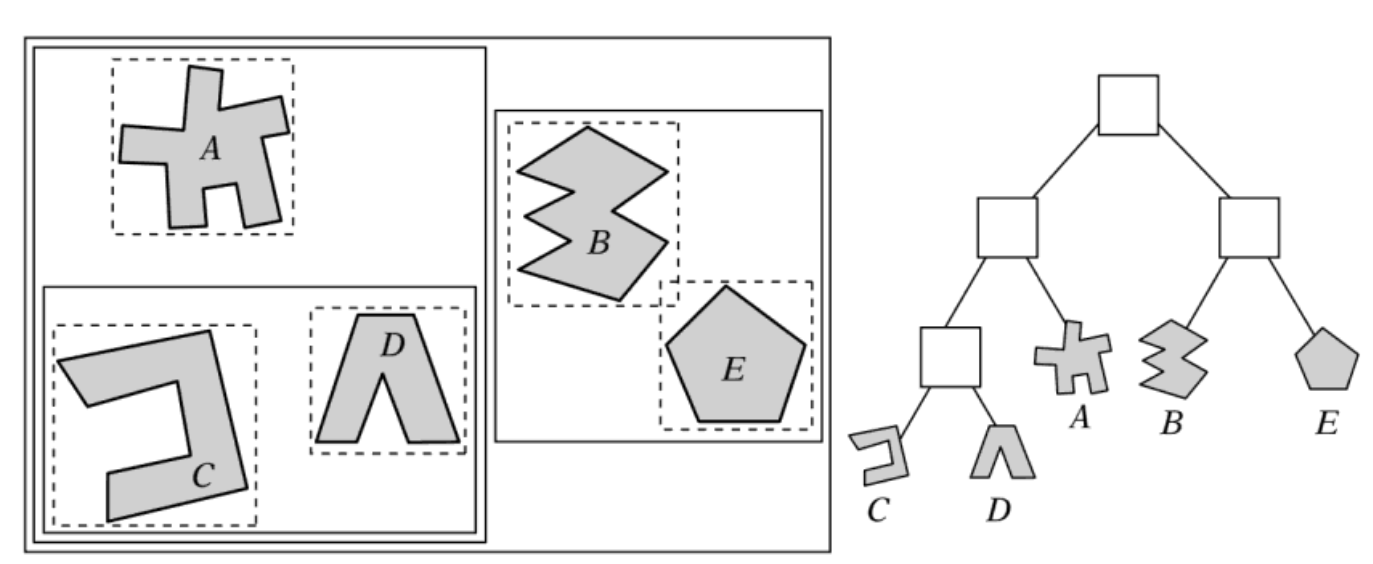
\includegraphics[width=0.85\textwidth]{Figures/BVH/BVH.png}
  \bicaption{BVH 加速结构示意图}{Schematic of BVH acceleration structure}
  \label{fig:bvh_structure}

  \small
  场景包围盒层次（左）与对应二叉树（右）。
\end{figure}

\subsection{CPU 光追加速：Intel Embree}
%% 写作思路：
%%   - Embree 定位：Intel 开发的高性能 CPU 光线追踪内核库，是本文 CPU Baseline 求解器
%%     （stardis-cpu）的几何相交后端。
%%   - 关键技术：
%%       · SIMD 并行（SSE4/AVX2/AVX-512）：同时对 4/8/16 条射线做 packet 遍历；
%%       · 多级 BVH（MBVH）：宽度为 4 或 8 的多叉 BVH，与 SIMD 寄存器宽度对齐；
%%       · 针对不同几何类型（三角形、曲线、细分曲面）的专用相交核。
%%   - 典型性能：单线程 ~$10^7$ rays/s 量级；多核线性扩展。
%%   - 本文角色：作为 Baseline 的几何后端，与第四章 GPU 后端进行性能对比。
%% [引用需求] \cite{waldEmbreeKernelFramework2014,EmbreeRayTracing}

Intel Embree 是 Intel 开发并开源的高性能 CPU 光线追踪内核库，也是本文 CPU 基准求解器的几何相交后端。Embree 针对现代 x86 处理器的 SIMD 指令集深度优化，通过射线包（ray packet）遍历模式实现单线程内的大幅并行加速：将宽度为 4、8 或 16 的多条射线打包为一个 packet，以 SSE4（128 位）、AVX2（256 位）或 AVX-512（512 位）SIMD 指令同时完成 packet 内所有射线与 BVH 节点（包围盒测试）或三角形（求交）的计算，每条向量指令处理多条射线，显著提升单位时钟周期内的浮点利用率。

与射线包遍历配套的底层加速结构为多叉 BVH（MBVH）：将二叉 BVH 扩展为 4 叉（QBVH，对应 SSE4）或 8 叉（OBHV，对应 AVX2）树，每个内部节点同时存储 4 个或 8 个子节点的 AABB 数据，恰好填满 SIMD 寄存器。包围盒测试时，一条向量指令可并行完成对全部子节点的 AABB 测试，将每个 BVH 节点的遍历代价压缩至极低。此外，Embree 针对三角形、线段曲线、细分曲面等不同几何图元类型提供了各自优化的专用求交内核，并支持用户注册自定义几何体类型的求交回调。

Embree 对外提供宽度分级的 C API：\texttt{rtcIntersect1()}（单条射线）、\texttt{rtcIntersect4/8/16()}（4/8/16 条射线 packet，分别对应 SSE4/AVX2/AVX-512）。宽接口在路径连贯、方向分布集中的渲染场景中可充分利用 SIMD 并行能力，达到接近理论峰值的吞吐量。然而，本文基准求解器在架构层面仅使用了 \texttt{rtcIntersect1()}——递归求解器为每条路径的每次状态转换各自独立发起一次同步查询，同一时刻从不存在多条路径的查询请求同时就绪，packet 接口所要求的一批方向同构射线在递归求解器中不可能被自然积累。这一约束正是 2.3.1 所描述的批量化障碍在 Embree 接口层面的直接体现：未能使用宽 packet 的原因不是 API 能力的缺失，而是上层递归求解架构决定了路径查询只能以宽度为 1 的形式提交。典型性能下，Embree 单条射线吞吐量约 $10^7$ 条/秒量级，开启 packet 模式后可进一步提升 4--8 倍；本文基准求解器受架构限制实际仅获得前者。在本文实验框架中，Embree 作为 CPU 基准后端的几何相交底层支撑，其性能将在第四章与基于 OptiX 的 GPU 批量查询后端进行系统性对比。

值得指出的是，Embree 本身是线程安全的：多个线程可安全地并发调用同一场景句柄的查询接口，无需额外加锁。本文基准求解器利用这一特性以 OpenMP 在粒子（路径）层面实现粗粒度并行——每个 OpenMP 线程独立运行一条路径的递归求解器并各自调用 \texttt{rtcIntersect1()}，线程间几乎不存在同步开销，从而在多核 CPU 上获得接近线性的加速比。本文 Wavefront 求解器同样依托 OpenMP 实现多线程并行，不同之处在于并行粒度从单条路径转变为任务队列：各 OpenMP 线程并行处理同类型挂起队列中的多个粒子状态，以批量方式驱动状态转换。两种架构均能随核心数的增加获得近线性的多核扩展能力，差异体现在对 SIMD 向量化与 GPU 批量卸载的利用程度上。

\subsection{GPU 硬件光追加速}
%% 写作思路：
%%   - RT Core 简介（Turing 架构起，NVIDIA 第一代，Ampere 为第二代）：专用固定功能单元，
%%     独立于 CUDA Core 和 Tensor Core，负责 BVH 遍历和光线-三角形求交。
%%   - 执行流程：CUDA kernel 发出 optixTrace() 调用 → 光线进入 RT Core 流水线 →
%%     BVH 遍历与求交完全在硬件中完成（对 CUDA 透明）→ 命中后触发用户可编程的 Closest-Hit
%%     / Any-Hit / Miss Shader（在 SM 上执行）。
%%   - 性能优势：RT Core 与 SM 并行工作，在高并发查询下吞吐量可达 Embree（单核）的 5~10 倍；
%%     本文实测结果见第四章。
%%   - OptiX 编程模型：NVIDIA 提供的光线追踪 API，封装 RT Core，提供 Pipeline/SBT（Shader
%%     Binding Table）机制，支持用户自定义 Intersection/Closest-Hit/Any-Hit/Miss 程序。
%% [图表需求] GPU SM 与 RT Core 协同流水线示意图（optixTrace→RT Core→Shader 执行流程）
%% [引用需求] \cite{parkerOptiXGeneralPurpose2010}

NVIDIA 自 Turing 架构（2018 年）起在 GPU 芯片中引入了专用的固定功能硬件单元 RT Core（Ray Tracing Core），Ampere 架构（2020 年）进行了第二代升级。RT Core 独立于传统的浮点 CUDA Core 和矩阵乘法 Tensor Core，专门负责两项操作：光线与 AABB 的相交测试，以及光线与三角形基于 Woop 坐标变换的精确求交。整个 BVH 遍历与三角形求交流水线在 RT Core 硬件中完成，不占用 SM 的可编程计算资源。

在 NVIDIA OptiX 框架下，GPU 光线查询的完整执行流程为：
\begin{enumerate}
    \item CUDA kernel 中调用 \texttt{optixTrace(handle, rayOrigin, rayDirection, tmin, tmax, ...)} 提交一条射线及其查询参数（SBT 偏移、Payload 寄存器等）；
    \item RT Core 从顶层加速结构（TLAS，Top-Level Acceleration Structure）向下执行 BVH 遍历，对每个叶节点中的三角形执行 Woop 坐标求交，并记录最近命中的 $t$ 值与几何属性；
    \item 遍历完成后，根据命中结果分发到对应的用户 Shader 程序，在 SM 上执行：
    \begin{itemize}
        \item \textbf{Closest-Hit Shader} --- 在最近命中时执行，处理交点信息进行路径更新;
        \item \textbf{Miss Shader} --- 在射线未命中任何几何体时执行，处理路径终止或背景采样;
        \item \textbf{Any-Hit Shader} --- 在每次潜在命中时执行（可选，用于透明度过滤）;
        \item \textbf{Intersection Shader} --- 用户自定义的自定义几何类型求交逻辑。
    \end{itemize}
\end{enumerate}
RT Core 遍历与 SM 执行异步并行：一条 Warp 提交 \texttt{optixTrace()} 后进入挂起态，SM 调度器立即切换到其他就绪 Warp 继续执行；RT Core 在后台完成遍历，结束后重新唤醒该 Warp 执行对应 Shader。这种流水线机制在大批量查询场景下使 RT Core 与 SM 的计算资源高度重叠，整体查询吞吐量远超纯软件 BVH 遍历。

OptiX 的高层接口以管线（Pipeline）和着色器绑定表（Shader Binding Table，SBT）两个概念为核心：Pipeline 定义本次查询涉及的 Shader 程序集合（CUDA PTX，由 OptiX JIT 链接）及遍历深度等配置参数；SBT 是设备端表格，每行对应一个几何实例及其绑定的 Shader 程序与参数，\texttt{optixTrace()} 通过携带的 SBT 偏移实现对不同几何体命中不同 Shader 的精确路由。正是这一灵活的 Pipeline/SBT 机制，使本文能够在保留 RT Core 硬件加速的前提下，为三类语义不同的几何查询分别构建独立管线。

\begin{figure}[htbp]
  \centering
  % 第一排：全芯片架构
  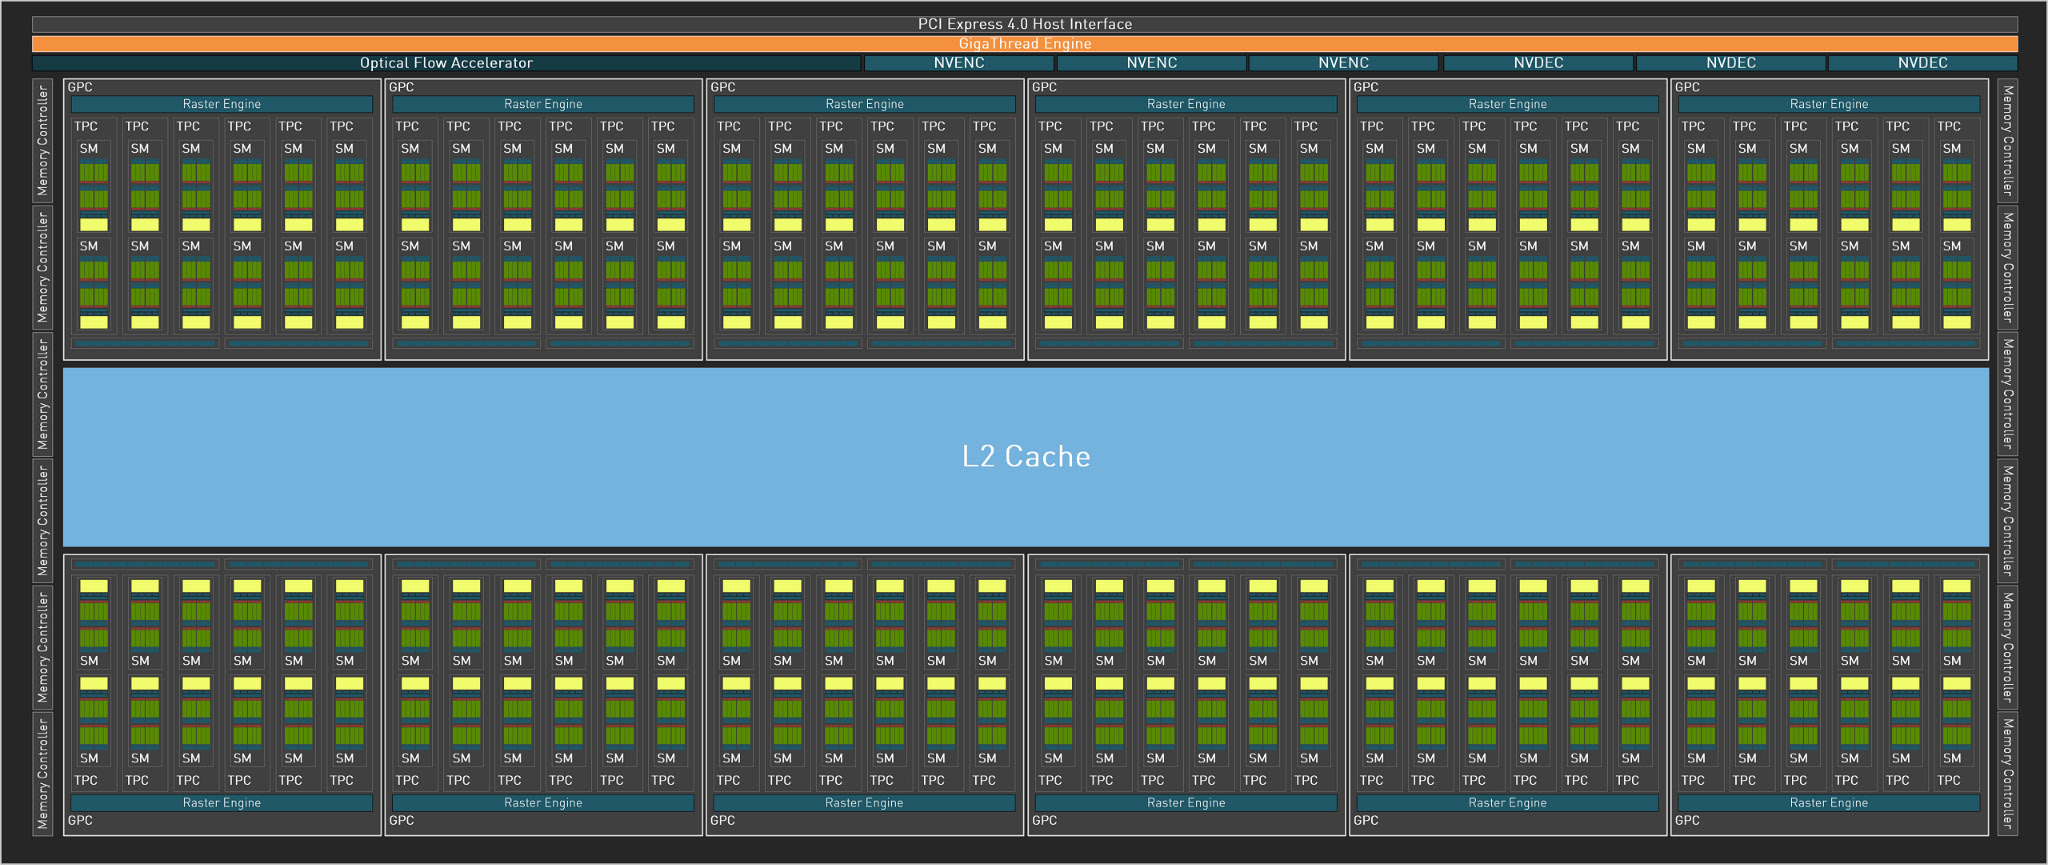
\includegraphics[width=0.95\textwidth]{Figures/GPU_Arch/AD102CoreArch.png}

  \vspace{6pt}
  % 第二排：GPC + SM
  \begin{subcaptiongroup}
  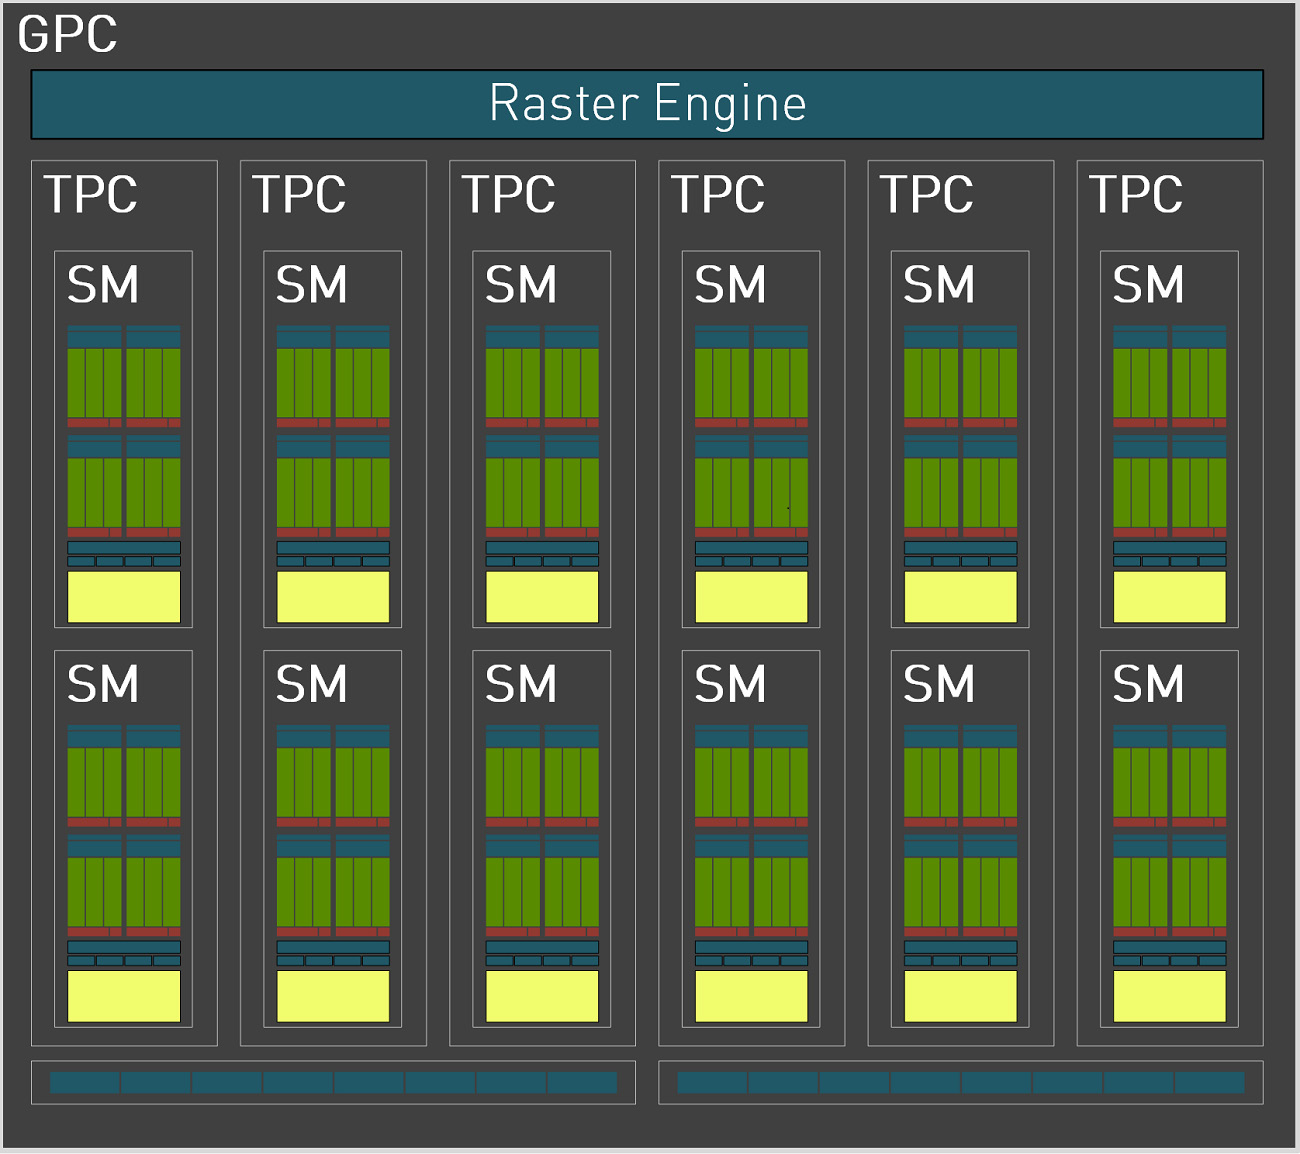
\includegraphics[width=0.54\textwidth]{Figures/GPU_Arch/AD102GPCDesign.png}
  \hfill
  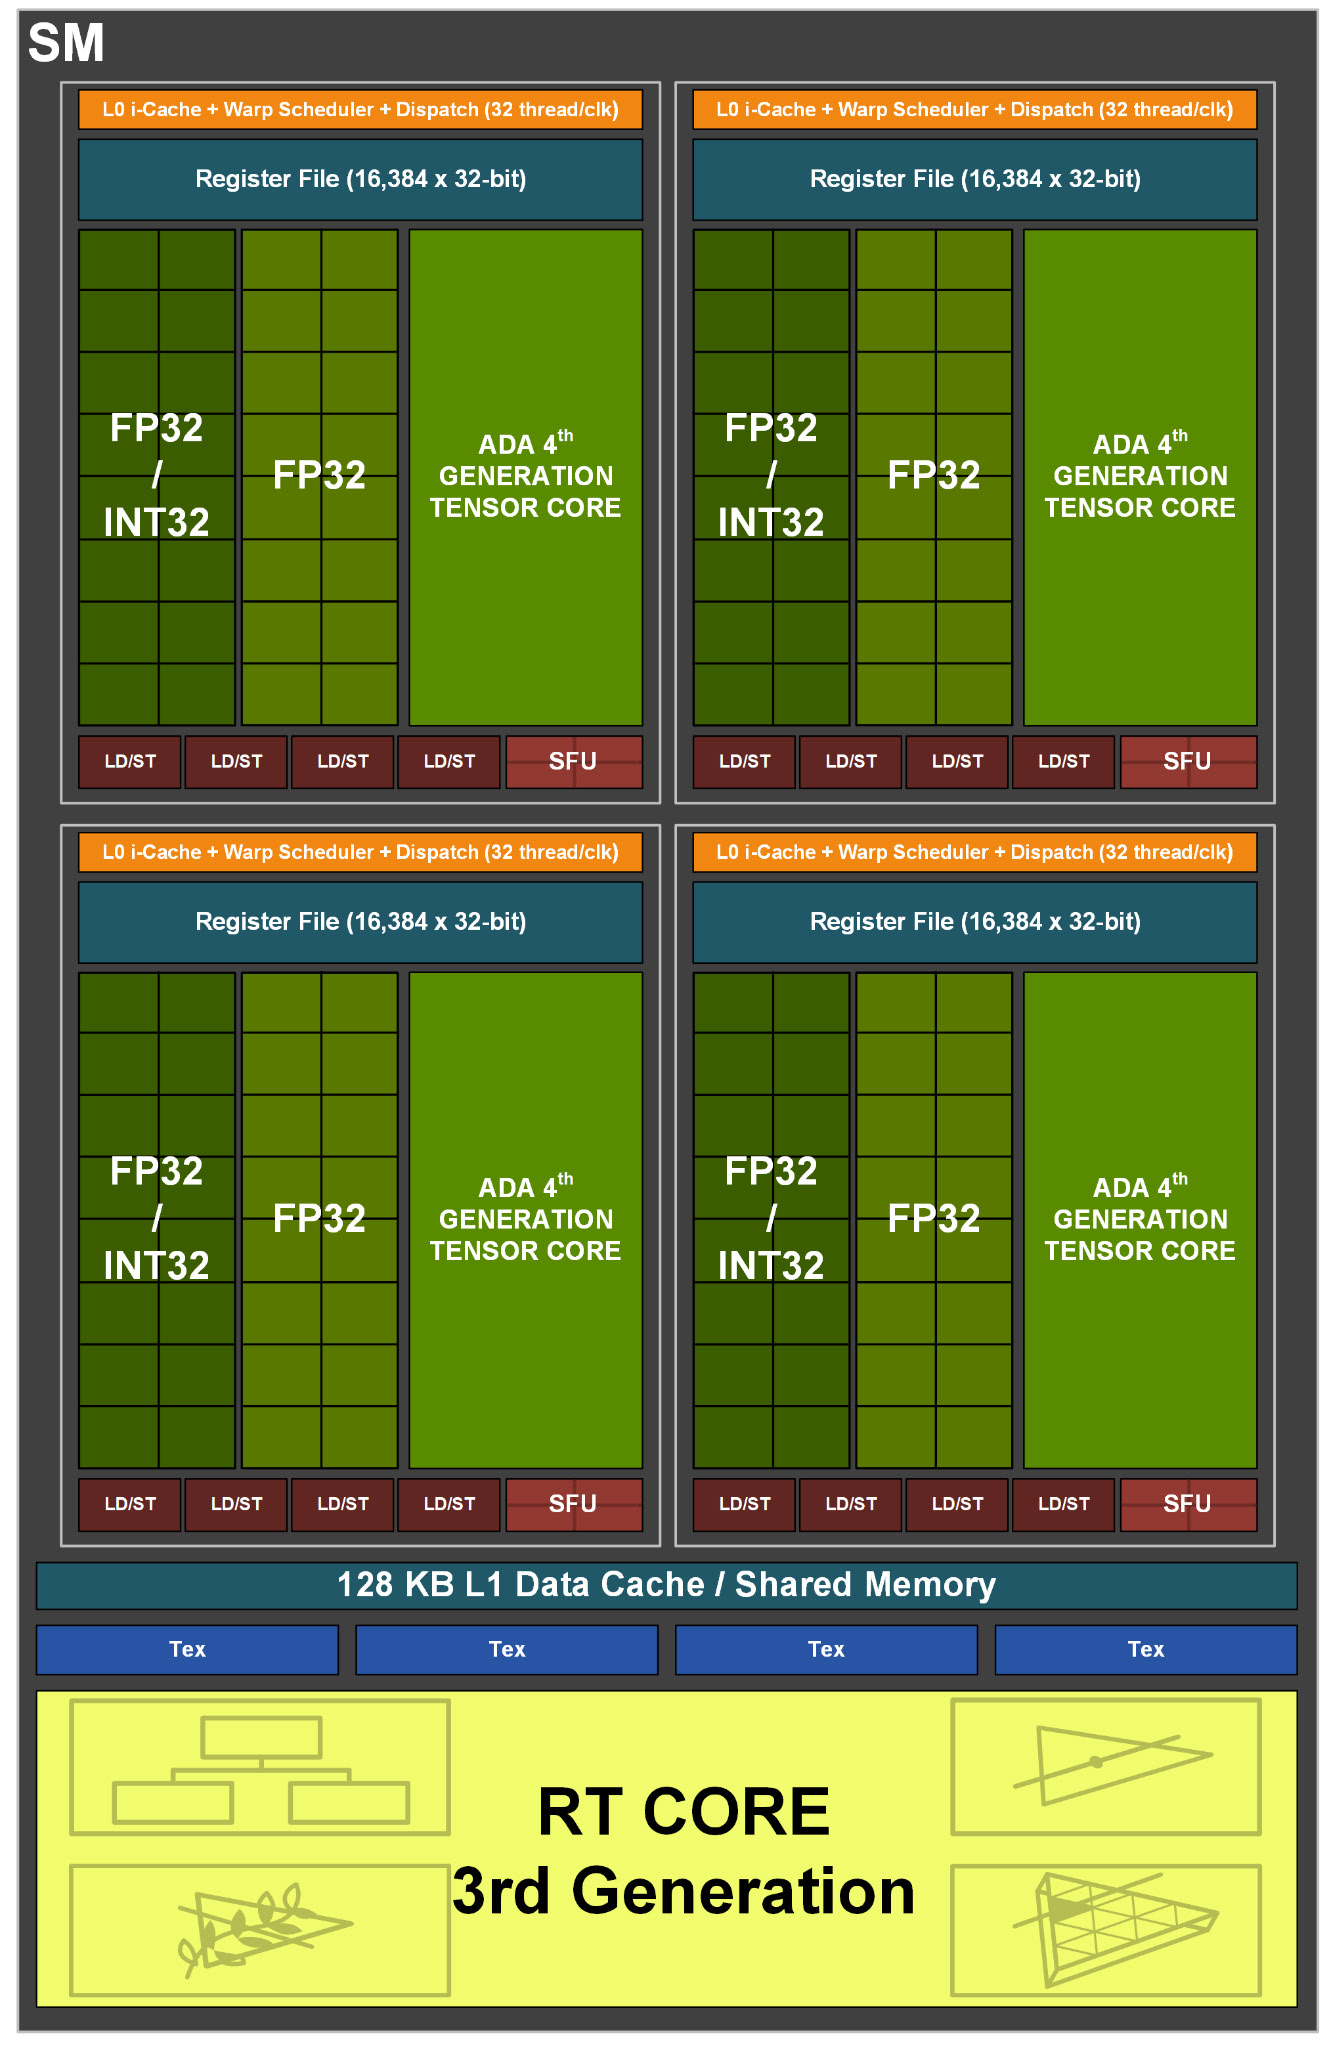
\includegraphics[width=0.32\textwidth]{Figures/GPU_Arch/AD102SMDesign.png}
  \end{subcaptiongroup}
  \bicaption{NVIDIA Ada Lovelace（AD102）GPU 架构层次\cite{nvidiaAdaGPUArchitecture2022}}{NVIDIA Ada Lovelace (AD102) GPU architecture hierarchy\cite{nvidiaAdaGPUArchitecture2022}}
  \label{fig:gpu_sm_rtcore}

  \small
  全芯片（上）、GPC（左下）与 SM（右下）。
  AD102 全芯片含 12 个 GPC、L2 Cache 及显存控制器；每个 GPC 包含 6 个 TPC，
  各 TPC 下辖 2 个 SM；每个 SM 含 4 个 Warp Scheduler、FP32/INT32 CUDA Core、
  第四代 Tensor Core 及底部的第三代 RT Core。
  RT Core 独立于 CUDA Core 执行 BVH 遍历与光线—三角形求交，
  SM 在 Warp 等待 RT Core 返回期间可调度其他就绪 Warp 继续计算。
\end{figure}

\subsection{本文涉及的几何查询类型}
%% 写作思路：
%%   - 说明热输运求解所需的几何查询并非只有标准"最近命中"光追，还需要另外两类特殊查询，
%%     这是第四章后端管线设计的直接需求来源。
%%   - 三类查询：
%%       (1) 最近命中光追（Closest-Hit）：沿光线方向找到第一个交点，用于辐射路径传播（主要查询）。
%%       (2) 最近面投影（Closest Point Projection，CP 查询）：给定空间点 $\mathbf{x}$，求
%%           场景表面上距其最近的三角形面片及精确投影位置——用于传导段 CND 布朗游走粒子的步长
%%           确定（距边界最近距离）和到达边界时触发 BND 事件。
%%           实现方式（基于 RTNN / PPoPP 2022）：将每个三角形预处理为以搜索半径膨胀的 AABB，
%%           查询点以"零长射线"（tmin=0, tmax=1e-16）发出，OptiX BVH 遍历找到所有含查询点的
%%           AABB，自定义 Intersection 程序以 Voronoi 区域法（双精度）计算到三角形精确距离，
%%           Payload 寄存器保留最近命中，输出距离、投影坐标、法向、面片索引。
%%       (3) 封闭腔体归属查询（Point-in-Enclosure，ENC 查询）：判断空间点是否位于某封闭腔体
%%           内部——用于确定给定位置的腔体归属（影响辐射边界条件的选取）。
%%           实现方式（两步）：
%%             Step 1: 对查询点执行 CP 查询，得到最近面片及其几何法向 $\hat{n}$；
%%             Step 2: 从查询点沿 $+X$ 方向发射单条标准 Closest-Hit 射线，读取命中法向 $\hat{n}_{\rm hit}$：
%%               射线未命中 → 外部（side=0）；
%%               命中：$\hat{n}_{\rm hit}.x < 0$ → 命中正面（外部，side=0）；
%%                      $\hat{n}_{\rm hit}.x > 0$ → 命中背面（内部，side=1）。
%%           即：法向点乘判侧，而非奇偶计数；使用标准 Closest-Hit 管线，非 Any-Hit。
%%   - 这三类查询将在第四章分别设计独立的 OptiX 管线（Pipeline）。
%% [引用需求] \cite{parkerOptiXGeneralPurpose2010}

由第 2.2 节与第 2.3 节的分析可知，耦合热输运路径追踪求解器所需的几何查询并非单一的标准最近命中光追，而是涵盖三类在物理语义上不同的查询，分别驱动路径状态机中的不同物理过程。这三类查询在第四章将各自设计独立的 OptiX 管线。

\textbf{第一类：最近命中光追（Closest-Hit Ray Tracing，RT 查询）。} 给定光线起点 $\mathbf{o}$ 与方向 $\hat{\mathbf{d}}$，在场景三角形网格中求第一个几何交点 $(\mathbf{x}^*, \hat{n}^*)$ 及对应的表面属性（材质编号、封闭腔体归属、发射率等）。该查询驱动 RAD 辐射、BND 各类界面步骤及 CND 传导步中凡涉及直接射线求交的过程，均向 RT 挂起队列提交请求，是三类查询中批量规模最大的一类，也是 OptiX/RT Core 最直接支持的查询类型。

\textbf{第二类：最近面投影（Closest Point Projection，CP 查询）。} 给定空间中任意点 $\mathbf{x}$，求场景表面上距其欧氏距离最小的点 $\mathbf{x}^* = \arg\min_{\mathbf{y} \in \partial\Omega}\|\mathbf{y} - \mathbf{x}\|$ 及其表面法向 $\hat{n}^*$。该查询仅用于传导段（CND）Walk-on-Spheres（WoS）游走路径变体的步长计算——WoS 算法需要当前位置至场景表面的最近距离来确定每步游走的球半径，并在粒子进入 epsilon-shell 时触发 BND 界面事件。

\textbf{第三类：封闭腔体归属查询（Point-in-Enclosure，ENC 查询）。} 给定空间中任意点 $\mathbf{x}$，判断其归属于哪个封闭腔体（Enclosure）。封闭腔体是 Stardis 场景模型的基本组织单元，每个腔体对应一组闭合固体表面，辐射边界条件的选取依赖于路径当前所处腔体的编号。ENC 查询通过向场景发射多条探测射线并依据命中面法向判侧来确定归属关系，主要用于 BND 界面事件中的腔体归属判断。

三类查询的语义、驱动过程与实现方案如表\,\ref{tab:query_types} 所示：

\begin{table}[htbp]
    \centering
    \bicaption{耦合热输运求解器所需的三类几何查询}{Three geometric query types in the coupled heat transport solver}
    \label{tab:query_types}
    \begin{tabular}{llll}
        \toprule
        查询类型 & 缩写 & 驱动过程 & 实现方式 \\
        \midrule
        最近命中光追 & RT & 各过程直接射线求交 & OptiX Closest-Hit 管线 \\
        最近面投影 & CP & CND 游走步长计算 & 场景表面最近点批量查询 \\
        封闭腔体归属查询 & ENC & BND 腔体归属判断 & 多方向探测射线 $+$ 法向判侧 \\
        \bottomrule
    \end{tabular}
\end{table}

\paragraph{建模假设与适用边界。}为聚焦于求解架构的并行化设计，本文蒙特卡洛耦合热输运框架采用三条工程简化假设，其在主流工业红外仿真任务中通常成立：（1）漫射灰体表面，即发射率与吸收率独立于波长且与方向无关；（2）透明非参与流体，即流体仅承担对流换热，不参与体积辐射散射或吸收；（3）线性化对流换热系数，即对流换热在工程温区内以恒定或弱温度依赖系数近似。上述假设的失效场景及对应扩展路径将在第六章展望中讨论。

\section{本章小结}

本章系统梳理了支撑本文工作的核心理论与技术基础。

第 2.1 节建立了耦合热输运的物理模型：分别阐述热传导、热辐射与热对流三种基本传热机制的物理规律及数学描述，并以联合能量平衡边界条件统一刻画三种机制在固-流界面处的耦合关系。其中热传导作为三维抛物型偏微分方程，以体积随机游走形式参与蒙特卡洛求解，几何查询开销远超其他过程，是驱动 GPU 硬件光追加速的核心动机。

第 2.2 节阐述了蒙特卡洛路径追踪在耦合热输运中的应用原理：从蒙特卡洛积分的基础理论出发，回顾经典正向追踪与反向路径追踪范式，重点介绍 Bati 等人将辐射、传导、对流三种机制统一至单一路径空间的耦合估计量框架，并以原始递归求解器实现为基准，指出其在批量化方面的结构性局限。

第 2.3 节与第 2.4 节分别介绍了两大工程技术基础。Wavefront 执行模型通过引入持久化路径状态与挂起队列，将状态推进与几何查询执行解耦，使大批量几何查询在架构层面成为可能，为第三章并行化求解器的设计提供范式依据。光线追踪与几何查询加速技术系统介绍了水密求交算法、BVH 层次加速结构，以及 Intel Embree（CPU 基准后端）与 NVIDIA OptiX/RT Core（GPU 硬件光追后端）两条工程路线，并明确了耦合热输运求解器所需的三类几何查询（RT、CP、ENC），为第四章 OptiX 后端三条管线的设计奠定直接基础。
%!TEX root = ../MainBody.tex

% 第三章
% ═══════════════════════════════════════════════════════════════════
% 写作思路（全章概要）：
%   本章是论文的核心贡献之一。逻辑线：
%     问题分析（DFS 局限）→ 理论等价变换（状态机抽象）→ 工程实现（Wavefront）→ 实验验证
%
%   对应项目：Stardis-GPU
%     Baseline: stardis-cpu/stardis-solver/ （原始 DFS 求解器）
%     Ours:     stardis-cus3d/stardis-solver/ （Wavefront 求解器）
%
%   核心论点：DFS 递归求解器虽然实现简洁，但其串行执行模型无法利用 GPU 的
%            大规模并行能力。通过将递归调用链抽象为有限状态机，并采用 Wavefront
%            批处理调度，可以在保持物理等价的前提下实现 GPU 加速。
% ═══════════════════════════════════════════════════════════════════
\chapter{基于 Wavefront 架构的并行化耦合热输运求解算法}
\label{chap:solver}
% 本章的写作思路是先分析现有DFS求解框架实现的和面向并行和GPU硬件加速的局限性，并提出求解任务的状态机等价表示，然后基于状态机表示提出Wavefront调度框架的CPU实现方案。并且，针对CPU Wavefront调度框架的调度开销，提出GPU stub进行同架构在GPU上进行调度成本测试的方案，并论证该方案的等效性。
%然后，在实验结果章节，首先对Wavefront框架进行物理一致性测试的数据分析，说明该框架解决仿真问题的正确性。然后进行

\section{引言}
%% 写作思路：
%%   - 简要回顾耦合热输运蒙特卡洛方法的计算特点（路径内多次光追、递归分支、高 SPP）
%%   - 点出核心矛盾：CPU DFS 架构串行执行 ↔ 海量路径并行需求
%%   - 概括本章目标：等价改造为 Wavefront 架构 + 实验验证正确性和性能
%%   - 本章组织结构导读
%% [篇幅需求] 约500字。

第 2.2.5 节描述了的逐路径的蒙特卡洛耦合热输运的递归路径追踪实现（下称递归求解器）。该实现以 \texttt{trace\_ray} 同步阻塞调用为基本操作单元——每次路径状态的推进均须等待一次几何查询的同步结果，路径从初始点到终止点的完整求解过程封装于一条连续的函数调用链中，中间状态隐式分布于调用栈的各层局部变量里。在算法层面，该实现正确描述了耦合传热的物理过程：辐射段（RAD）、界面事件（BND）、固体传导（CND）、对流换热（CNV）四类状态间的概率转移，单路径串行执行时产生统计无偏的辐亮度估计量。

然而，红外仿真的实际计算规模揭示了一个结构性矛盾。从查询需求来看，每条路径在其完整生命周期内需经历数十万次异构几何查询：辐射弹射与遮挡检测依赖射线最近命中查询（RT 查询），固体传导随机游走的步长界估计依赖最近面投影查询（CP 查询），界面事件的腔体归属判定依赖封闭腔体成员查询（ENC 查询）。三类查询在单条路径内反复交替出现；同时，为达到工程所需的收敛精度，每个探测器像素需要数十乃至数百条独立路径，使总查询量达数十亿量级。然而从执行结构来看，递归求解器的同步阻塞模型决定了上述查询只能以宽度为 1 的方式逐条串行提交：路径调用 \texttt{trace\_ray} 时必须阻塞等待当次结果返回后才能确定后续物理状态，其他路径的查询请求在此等待期间无从积累——海量路径的几何查询调用在架构层面被完全分散，几何查询后端的大批量并行吞吐能力因此无从发挥（详见3.3）。

本章目标是在保持物理等价的前提下，从架构层面消解上述矛盾，将原始递归求解器等价改造为耦合输运状态机 Wavefront 求解器（下称 Wavefront 求解器）。改造的核心思路（参见第 2.3 节 Wavefront 范式原理）是：将路径状态从调用栈显式提取为持久化结构体，把状态推进与几何查询执行解耦为两个独立阶段——路径推进至查询节点后即进入挂起状态，系统继续推进其余路径；待本轮路径池中的查询请求整批积累完毕，统一提交至查询后端并行处理；结果返回后各路径从挂起点恢复继续前进。Wavefront 架构在设计上对执行设备不做假设——状态推进与查询执行均可在任意计算设备上运行；本章选择 CPU 调度 $+$ GPU 查询的混合实例化，旨在以最小代码改动验证架构正确性并定位性能关键路径。在此上层架构基础上，本章进一步设计了以 CPU 承担路径状态调度、以 GPU 作为批量几何查询执行后端的 CPU-GPU 混合框架（后端管线的详细设计见第四章），并引入双流 Ping-Pong 异步调度机制以隐藏设备间通信延迟。最后，从物理一致性与运行性能两个维度对改造结果进行实验验证。

本章内容组织如下：第 3.2 节从算法层面推导 Wavefront 状态机设计的全部约束，包括挂起点分析、路径状态字段集与三类几何查询的分类依据；第 3.3 节从代码结构角度剖析递归求解框架无法批量化的根本原因；第 3.4 节提出状态机等价变换方案、Wavefront 执行模型以及 CPU-GPU 混合架构设计；第 3.5 节报告物理一致性验证与性能评估的实验结果；第 3.6 节总结本章贡献并引出第四章 OptiX 查询后端的独立设计。

\section{耦合热输运路径追踪算法规约}
%% 本节从并行化设计视角重新审视 Algorithm 1，推导 Wavefront 状态机的全部设计约束：
%% 挂起点分析、路径状态字段集、三类查询类型。
%% 不重复第二章内容，着重从约束导出而非求解描述。
%% [篇幅需求] 约 800 字 + 两张表。
%% [图表占位] 挂起点位置标注图（待 2.2.5 伪代码确定后添加）

第 2.2.5 节以算法~\ref{alg:bnd}--\ref{alg:cnv} 展示了耦合热输运蒙特卡洛递归求解器的四个互递归子例程（BND、RAD、CND、CNV），着眼于正确性——描述各物理模态如何按概率转移、每次几何查询如何驱动路径前进。本节从并行化设计角度重新审视同一算法，着重回答：针对该算法的任何并行化实现需满足哪些固定约束——"算法需要持久化哪些路径信息"以及"算法涉及哪些可独立批量执行的几何查询操作"。这些约束完全由算法的物理逻辑决定，与具体的并行化机制无关，是本章第 3.4 节状态机设计的直接依据。

本节将算法~\ref{alg:bnd}--\ref{alg:cnv} 中每一次几何查询调用视为一个挂起点：若在此处将"同步等待查询结果"替换为"记录查询请求、挂起路径、等待批量结果回填"，路径在挂起瞬间须将完整的算法中间状态序列化至外部结构体 \texttt{path\_state} 以备后续恢复。因此，挂起点的数量与类型决定了：(1) 状态枚举 \texttt{path\_phase} 需要多少对挂起/恢复状态；(2) 每类查询需要哪种专用挂起队列；(3) \texttt{path\_state} 结构体须保存哪些字段。

\subsection{实例分析一：辐射传播段的查询挂起点}

以辐射传播（RAD）状态下的弹射步为例，说明几何查询如何嵌入递归执行流，并由此推导挂起时的持久化需求。递归实现中，辐射随机游走的核心函数为 \texttt{find\_next\_fragment}（源码 \texttt{sdis\_heat\_path\_radiative\_Xd.h}），其从当前位置沿采样方向寻找下一命中界面，调用链简化如下：

\begin{quote}\small
\texttt{trace\_radiative\_path(scn, dir, ctx, rwalk, rng, T)}\\
\hspace*{1.5em}\texttt{$\rightarrow$ find\_next\_fragment(scn,\,rt\_pos,\,in\_dir,\,in\_hit,\,time,\,enc\_id,\,...)}\\
\hspace*{3em}\textbf{[*]}\;\texttt{trace\_ray(scn,\,rt\_pos,\,in\_dir,\,$\infty$,\,enc\_id,\,in\_hit,\,\&hit)}\\
\hspace*{5em}/* 同步阻塞，等待最近命中结果 */\\
\hspace*{3em}\texttt{interf = scene\_get\_interface(scn, hit.prim.prim\_id)}\\
\hspace*{3em}\texttt{setup\_fragment(\&frag,\,pos,\,in\_dir,\,time,\,N,\,\&hit)}\quad/* 使用 hit */\\
\hspace*{3em}\texttt{check\_interface(interf, \&frag, ...)}
\end{quote}

标注 [*] 的 \texttt{trace\_ray} 调用即 RT 查询挂起点。若将同步阻塞改为"提交查询请求、挂起路径、等待批量回填"，则路径在挂起瞬间须持久化以下信息才能在结果到达后正确恢复：
\begin{itemize}[nosep]
  \item \texttt{rt\_pos}：射线起点（查询参数；恢复后计算命中位置 $\mathbf{x}_\text{hit} = \texttt{rt\_pos} + d\cdot\texttt{hit.distance}$ 时仍需）；
  \item \texttt{in\_dir}：传播方向（查询参数；恢复后调用 \texttt{setup\_fragment} 时仍需）；
  \item \texttt{enc\_id}：当前腔体编号（查询过滤参数；同时决定后续界面物理参数查找）；
  \item \texttt{in\_hit}：前序命中记录（自相交过滤参数，防止再次命中出发面）；
  \item \texttt{time}：仿真时刻（\texttt{setup\_fragment} 在恢复后调用时需要此值）；
  \item 相位标识：标记"此路径在 RAD 弹射 RT 查询处挂起"，恢复后直接跳入命中处理逻辑。
\end{itemize}

\subsection{实例分析二：Walk-on-Spheres 传导段的双重查询挂起点}

以传导（CND）状态下 Walk-on-Spheres 游走步为例，说明同一函数内存在两类不同性质查询挂起点的情形。WoS 游走函数 \texttt{sample\_next\_position}（\texttt{sdis\_heat\_path\_conductive\_wos\_Xd.h}）每步首先需确定当前位置至最近几何面的距离以确定球面半径，其简化调用链如下：

\begin{quote}\small
\texttt{sample\_next\_position(scn, rwalk, rng, delta, \&distance)}\\
\hspace*{1.5em}\textbf{[A]}\;\texttt{scene\_view\_closest\_point(view,\,wos\_pos,\,$\infty$,\,NULL,\,\&hit)}\\
\hspace*{3em}/* CP 查询，同步等待最近面距离 */\\
\hspace*{1.5em}\texttt{wos\_distance = hit.distance}\\
\hspace*{1.5em}\textbf{if} \texttt{wos\_distance} $\leq\varepsilon_\text{shell}$\texttt{(delta):}\quad\texttt{setup\_hit\_wos(...)}\\
\hspace*{1.5em}\textbf{else:}\quad\texttt{dir} $\leftarrow$ \texttt{sphere\_uniform(rng);\quad pos = rwalk->vtx.P + dir * wos\_distance}\\
\hspace*{3em}\texttt{check\_diffusion\_position(scn, rwalk->enc\_id, delta, pos)}\\
\hspace*{3em}\textbf{if} invalid:\\
\hspace*{4.5em}\textbf{[B]}\;\texttt{scene\_view\_trace\_ray(view,\,rt\_pos,\,rt\_dir,\,...,\,\&hit\_rt)}\\
\hspace*{6em}/* RT 回退查询，同步等待 */
\end{quote}

调用点 [A]（CP 查询）挂起时须持久化：\texttt{rwalk->vtx.P}（当前游走位置，查询原点）、\texttt{rwalk->enc\_id}（所属腔体，界面侧判断依据）、\texttt{delta}（步长参数，决定 $\varepsilon$-shell 阈值）及 \texttt{rng} 状态（恢复后方向采样需继续此随机序列）。

调用点 [B]（RT 查询，仅在 [A] 恢复后位置合法性验证失败时发生）与 [A] 共享大部分上下文字段，但须额外保存 [A] 恢复后已采样的 \texttt{dir}（回退射线方向）及候选位置 \texttt{pos}。两个调用点虽同处一个函数，却对应不同的查询类型，须分别为其分配独立的相位标识。

两段实例揭示了一个通用规律：递归调用栈中每一个几何查询调用点，其挂起时所需持久化的状态集合，精确等于该调用点所在帧及全部祖先帧中“查询返回后仍需使用的局部变量”之并集。将此分析方法扩展到 \texttt{stardis-cpu} 递归求解器（\texttt{sdis\_heat\_path\_*.h} 系列）中全部几何查询调用点，即可完整枚举所有挂起点及其持久化需求。

\subsection{全算法挂起点枚举与三类查询分类}

对递归求解器（\texttt{stardis-cpu}）中全部 \texttt{scene\_view\_trace\_ray} 和 \texttt{scene\_view\_closest\_point} 调用点逐一分析，共识别出 19 个 几何查询挂起点，按查询操作类型分属三类，如表~\ref{tab:suspension-points} 所示。表中同时标注了 3.4 Wavefront 实现为每个挂起点赋予的状态名称，此处提前列出以便建立对照关系。

\begin{table}[htbp]
  \centering
  \bicaption{递归求解器几何查询调用点与查询类型分类}{Recursive solver geometric query call sites and query type classification}
  \label{tab:suspension-points}
  \small
  \begin{tabular}{p{4.6cm}cll}
    \toprule
    3.4 对应挂起状态（\texttt{path\_phase}） & 类型 & 所在物理过程 & 查询描述 \\
    \midrule
    \multicolumn{4}{l}{\textit{RT 查询——射线最近命中（14 个调用点）}} \\
    \midrule
    \texttt{PATH\_RAD\_TRACE\_PENDING}         & RT & 辐射传播       & 余弦采样方向最近命中，1 条 \\
    \texttt{PATH\_COUPLED\_BOUNDARY\_REINJECT} & RT & 界面重注入（遗留）& 重注入候选方向，1 条 \\
    \texttt{PATH\_BND\_SS\_REINJECT\_SAMPLE}   & RT & 固-固界面重注入  & 双侧各 2 方向，共 4 条 \\
    \texttt{PATH\_BND\_SF\_REINJECT\_SAMPLE}   & RT & 固-流界面重注入  & 候选重注入方向，2 条 \\
    \texttt{PATH\_BND\_SF\_NULLCOLL\_RAD\_TRACE} & RT & 固-流零碰撞辐射  & 零碰撞子辐射路径，1 条 \\
    \texttt{PATH\_BND\_SFN\_RAD\_TRACE}        & RT & PicardN 子路径  & 递归子辐射路径弹射，1 条 \\
    \texttt{PATH\_BND\_EXT\_DIRECT\_TRACE}     & RT & 外部净通量（直射）& 点光源阴影射线，1 条 \\
    \texttt{PATH\_BND\_EXT\_DIFFUSE\_TRACE}    & RT & 外部净通量（漫射）& 漫反射弹射方向，1 条 \\
    \texttt{PATH\_BND\_EXT\_DIFFUSE\_SHADOW\_TRACE} & RT & 外部净通量（遮挡）& 漫反射遮挡射线，1 条 \\
    \texttt{PATH\_COUPLED\_COND\_DS\_PENDING}  & RT & delta-sphere 传导（遗留）& 随机方向对，2 条 \\
    \texttt{PATH\_CND\_INIT\_ENC}              & RT & 传导路径初始化   & 腔体归属查询射线，1 条 \\
    \texttt{PATH\_CND\_DS\_STEP\_TRACE}        & RT & delta-sphere 步长估计 & 方向对步长射线，2 条 \\
    \texttt{PATH\_CND\_WOS\_FALLBACK\_TRACE}   & RT & WoS 传导回退（即[B]）& Walk-on-Spheres 回退射线，1 条 \\
    \texttt{PATH\_CNV\_STARTUP\_TRACE}         & RT & 对流路径初始化   & 对流域探针射线，1 条 \\
    \midrule
    \multicolumn{4}{l}{\textit{ENC 查询——封闭腔体归属（3 个调用点）}} \\
    \midrule
    \texttt{PATH\_ENC\_QUERY\_EMIT}            & ENC & 腔体归属（主方案）& 6 条轴对齐旋转射线投票 \\
    \texttt{PATH\_ENC\_QUERY\_FB\_EMIT}        & ENC & 腔体归属（随机回退）& 1 条随机方向回退射线 \\
    \texttt{PATH\_ENC\_LOCATE\_PENDING}        & ENC & 腔体归属（BVH 定位）& BVH 最邻近基元点定位 \\
    \midrule
    \multicolumn{4}{l}{\textit{CP 查询——最近面投影（2 个调用点）}} \\
    \midrule
    \texttt{PATH\_CND\_WOS\_CLOSEST}           & CP & WoS 步长上界（即[A]）& 最近三角面片投影距离 \\
    \texttt{PATH\_CND\_WOS\_DIFFUSION\_CHECK}  & CP & WoS 扩散位置验证  & 候选新位置近面合法性 \\
    \bottomrule
  \end{tabular}
\end{table}

三类查询的物理必要性各自独立。RT 查询（14 个调用点）是路径追踪算法的基本操作，覆盖辐射弹射、各类界面重注入、传导步长估计、对流初始化及外部净通量子流程，无法回避。ENC 查询（3 个调用点）是耦合热输运的特有需求：纯辐射渲染无需腔体归属，而多腔体耦合场景中每个封闭腔体赋予独立的发射率 $\varepsilon$、导热系数 $\lambda$ 和对流系数 $h$，路径在 BND 界面事件时须先确定所属腔体才能查找正确物理参数。CP 查询（2 个调用点）是 Walk-on-Spheres 传导游走的直接需求：WoS 步长上界等于游走点至最近面的投影距离，直接查询比等价的随机双向射线对方案（delta-sphere）对稠密固体内部的传导步更为高效，两种方案在实现中并存以适应不同几何环境。三类查询的划分依据是耦合热输运的物理计算需求，与第四章 GPU 后端如何高效执行这些查询是独立的两个问题。

\subsection{路径状态的最小必要字段集合}

对全部 19 个调用点按上述实例分析方法逐一梳理"返回后仍需使用的局部与祖先帧变量"并取并集，可归纳出 \texttt{path\_state} 结构体的最小必要字段集合：其一，几何与传播状态（当前位置、传播方向、当前腔体编号、前序命中记录），覆盖全部 RT/ENC/CP 调用点；其二，物理路径参数（仿真时刻、Picard 分支计数、温度估计量及完成标志），覆盖 BND 与终止判断调用点；其三，随机数状态（per-path CBRNG 密钥与计数器），覆盖所有调用点以确保路径恢复后随机序列的确定性延续；其四，过程局部变量联合体（WoS 步长参数、BND 各分支临时量、PicardN 子路径递归栈等），仅在对应物理过程的调用点中需要；其五，相位标识，标记路径当前挂起在哪个调用点，作为恢复时的状态机分发依据。上述字段集合与递归求解器执行到该调用点时整个调用栈的局部变量信息量完全等价——每个字段均能追溯到至少一个调用点的恢复需求，无冗余字段，无遗漏字段。

以两类字段为例说明该映射关系。几何与传播状态（当前位置、传播方向、当前腔体编号）是全部 19 个挂起点共同依赖的恢复前提——任何挂起点的查询结果到达后，路径恢复的第一步均为读取当前位置以确定后续物理逻辑的空间上下文，因此该类字段覆盖全部挂起点。过程局部变量联合体则与特定挂起点形成精确对应：BND-SF 子模块在 $\delta$ 偏移重注入射线发射后挂起（挂起点 \texttt{PATH\_BND\_SF\_REINJECT\_SAMPLE}），恢复时需读取命中结果以判定界面类型并选择后续分支，对应字段为 \texttt{bnd\_sf\_reinject\_hit}；WoS-CND 在最近面投影查询后挂起，恢复时需读取当前球面半径以计算下一步步长，对应字段为 \texttt{wos\_local.r\_sphere}。二者分别属于 BND 和 CND 物理过程的局部变量，仅在各自对应的挂起点中被引用，存储于联合体的不同分支中。该映射关系在全部挂起点上成立：每个字段至少被一个挂起点的恢复逻辑引用（无冗余），每个挂起点的恢复逻辑所需变量均被某字段覆盖（无遗漏）。字段的具体定义与布局优化将在 3.4 中展开。

\subsection{小结}

以递归求解器（\texttt{stardis-cpu}）实现为出发点，通过对辐射传播段和 WoS 传导段的具体实例分析，建立了"递归调用点 $\rightarrow$ 挂起所需持久化状态"的分析方法，并将其推广到全算法的 19 个几何查询调用点，识别出三类查询（RT、ENC、CP）和五类字段。这些约束完全由算法的物理计算需求决定，是耦合热输运路径追踪算法在任何并行化实现方向上提出的固有规约，是 3.3 节状态机设计的直接依据。

\section{Wavefront耦合热输运求解器实现}

第 2.3 节的分析指出，递归求解框架存在四大结构性障碍——调度粒度过大（障碍 A）、路径状态不可持久化（障碍 B）、查询请求无法批量积累（障碍 C）以及复合物理分支无法拆分调度（障碍 D），四者的共同根因是路径状态与执行控制流的隐式耦合。消解该根因需在架构层面引入两个结构性前提：

\begin{itemize}[nosep]
  \item \textbf{前提 A（可挂起性）}：路径执行推进至任意几何查询调用点时，其完整的算法中间状态可以持久化到外部结构体 \texttt{path\_state}，查询结果到达后能够从中断点无损恢复——即路径状态与执行控制流完全解耦。
  \item \textbf{前提 B（可聚合性）}：多条处于挂起等待状态的路径的查询请求，可以从各自的 \texttt{path\_state} 中提取并聚合为连续缓冲区，统一提交至查询后端并行处理；状态推进阶段与查询执行阶段在时序上完全解耦。
\end{itemize}

两个前提共同支撑了 Wavefront 执行范式：以固定大小路径池为中心数据结构，将原递归求解器"对每条路径递归到底"的一次性处理模式，重构为持续迭代的推进→收集→批量执行→回填四阶段循环。每次迭代将路径池中全部活跃路径各推进一步至下一个查询节点，收集本轮各路径的查询请求后统一提交，待批量结果返回后各路径从中断点恢复，继续推进至下一节点——如此反复，直至所有采样任务完成。

本节的三个子节分别对应两个前提的落地与组合利用：\S\ref{subsec:fsm} 通过递归到 FSM 的等价变换，构造满足前提 A 的显式路径状态机，将路径的全部中间状态序列化为可持久化的 \texttt{path\_state} 结构体；\S\ref{subsec:wf-model} 以前提 A 为基础，建立满足前提 B 的 Wavefront 主循环执行模型，设计路径池管理、查询批次组织与等价性保证机制；\S\ref{subsec:hybrid-arch} 利用主循环形成的批量请求/批量响应接口边界，设计 CPU-GPU 两角色异构调度架构，并引入双流 Ping-Pong 机制以隐藏跨设备传输延迟。

\subsection{耦合热输运求解的状态机抽象}
\label{subsec:fsm}

蒙特卡洛耦合热输运路径穿行于由四类物理段组成的耦合热输运过程：辐射传播段（RAD）、界面耦合事件（BND）、传导游走段（CND）和对流换热段（CNV）。路径从探测器出发经 RAD 弹射到达固体表面后进入 BND，BND 按界面类型和概率将路径分发至 CND、CNV 或继续 RAD，形成链式结构：
\begin{equation*}
  \text{相机} \;\xrightarrow{\mathrm{RAD}}\; \text{界面}
  \;\xrightarrow{\mathrm{BND}}\;
  \begin{cases}
    \mathrm{CND}\;\text{（固体传导）} \;\to\; \text{界面} \;\xrightarrow{\mathrm{BND}}\; \cdots \\
    \mathrm{CNV}\;\text{（流体对流）} \;\to\; \text{终止} \\
    \mathrm{RAD}\;\text{（继续弹射）} \;\to\; \cdots
  \end{cases}
\end{equation*}
每类物理段的求解算法中蕴含若干几何查询需求（RT 射线命中、CP 最近面投影、ENC 腔体归属），构成 FSM 必须覆盖的挂起点集合。图~\ref{fig:coupled_path} 直观展示了路径在多层嵌套场景中的完整物理生命历程。

\begin{figure}[htbp]
  \centering
  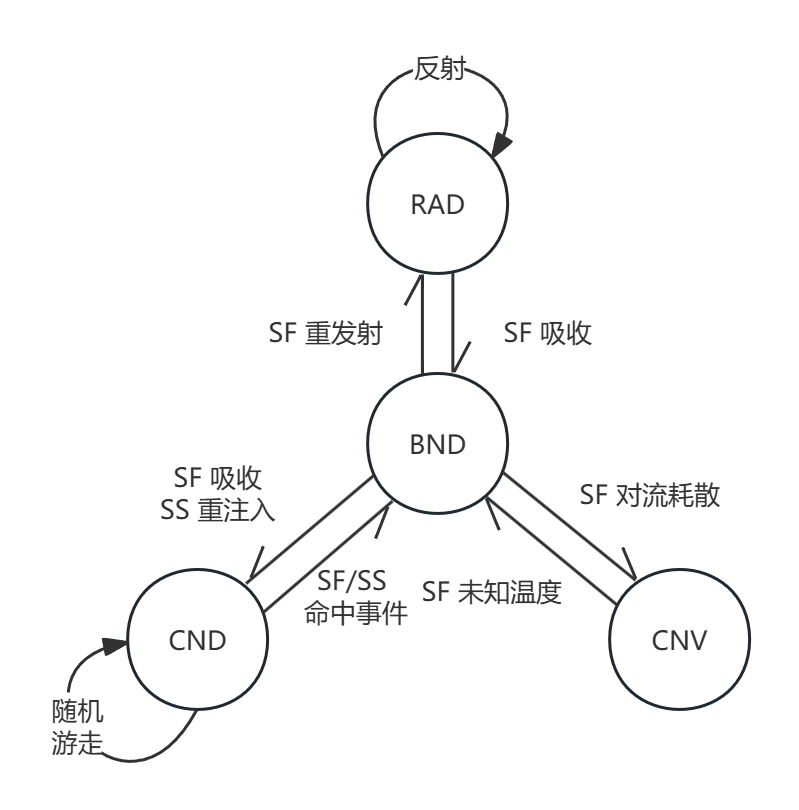
\includegraphics[width=1.0\textwidth]{Figures/Coupled_Path/CoupledPath.png}
  \bicaption{多层嵌套场景耦合热输运蒙特卡洛路径示意图}{Schematic of Monte Carlo path propagation in a multi-layer nested coupled heat transport scene}
  \label{fig:coupled_path}

  \small
  场景为二维截面：外部环境~Fluid~A 中放置固体外壳~Solid~A（$\lambda_A$，橙色），
  其内部包含封闭流体腔~Fluid~B（蓝色）和内嵌固体~Solid~B（$\lambda_B$，绿色），
  Solid~B 内进一步嵌套已知温度固体~Solid~C（浅黄色）。
  路径自探测器出发经辐射传播（RAD）命中~Solid~A 外表面（BND~1），
  渗透进入固体后执行传导随机游走（CND）。
  游走过程中的 $\delta$-球面吸附步可命中三类界面，分别展示：
  反射/对流出射至外部环境（BND~4）、
  再发射穿越封闭腔体（BND~2 $\to$ BND~3）、
  固-固跨壁传导进入相邻固体（BND~5 $\to$ BND~6）。
  图中同时展示全部四种终止条件：
  辐射逃逸（Miss）、对流耗散（Dissipation）、时间回溯（Time）和已知温度（Known Temperature）。
\end{figure}

本节将递归求解器的隐式调用栈状态等价转换为显式有限状态机（FSM）——任何有限递归调用图均可通过将函数返回地址显式化为状态枚举、调用栈局部变量显式化为结构体字段来完成此变换，这是算法等价变换的基本方法。基于细粒度状态机的耦合热路径计算过程可在任意几何查询阶段将完整路径状态持久化至外部结构体并完成挂起，待查询结果到达后从中断点无损恢复执行。以下逐模块展开各物理过程的 FSM 状态组设计，每个模块遵循"物理方程 $\to$ 蒙特卡洛求解步骤 $\to$ 几何查询需求 $\to$ FSM 状态产出"的统一范式。

\subsubsection{辐射传播模块（RAD）：渲染方程驱动的多次弹射}

辐射传播段（RAD）是耦合路径的"外层骨架"：路径从红外探测器出发，在透明流体中沿直线传播，反复在固体表面弹射，直至被吸收或射线未命中任何几何体（Miss）。其物理基础是灰体漫射表面假设下渲染方程（式~\eqref{eq:rendering}）的简化形式——路径追踪对其作 Neumann 级数展开，得到辐射温度的无偏估计量：路径从 $\mathbf{x}$ 沿 $\boldsymbol{\omega}$ 出发，经若干次弹射最终到达固体终止点 $\mathbf{x}_\Gamma$ 的表面温度之期望值。蒙特卡洛逐次采样的弹射规则为：命中表面后以概率 $\varepsilon$ 吸收（终止弹射段），以概率 $(1-\varepsilon)$ 按余弦分布 $\boldsymbol{\omega}' \sim (\boldsymbol{\omega}' \cdot \hat{n})/\pi$ 漫反射继续弹射；若射线未命中任何几何体（Miss），路径终止于预设的环境辐射温度 $\theta_{R,\text{env}}$。

RAD 模块每次弹射产生 1 个 RT 查询（射线最近命中），是全部 FSM 物理模块中结构最简单的。命中后的处理逻辑为：Miss 时以 $\theta_{R,\text{env}}$ 终止路径；命中 Dirichlet 边界时以已知温度直接终止；命中温度待求面时以 $\varepsilon$ 概率吸收、$(1-\varepsilon)$ 概率反射继续弹射。

\textbf{RAD 与 BND 的管理边界}：上述 $\varepsilon$-吸收/$(1-\varepsilon)$-反射是渲染方程 Neumann 展开中的截断采样，本质上属于 RAD 弹射循环的一部分——它决定弹射是否继续。当吸收事件发生后（RAD 弹射段终止），路径转入 BND 模块执行界面处的三模态能量分配（$P_\text{cond}/P_\text{conv}/P_\text{rad}$），决定后续进入 CND、CNV 还是开启新一段 RAD 弹射。因此，RAD 的"吸收出口"即是 BND 的"入口"，两者边界在 $\varepsilon$-吸收决策完成之时。

\begin{figure}[htbp]
  \centering
  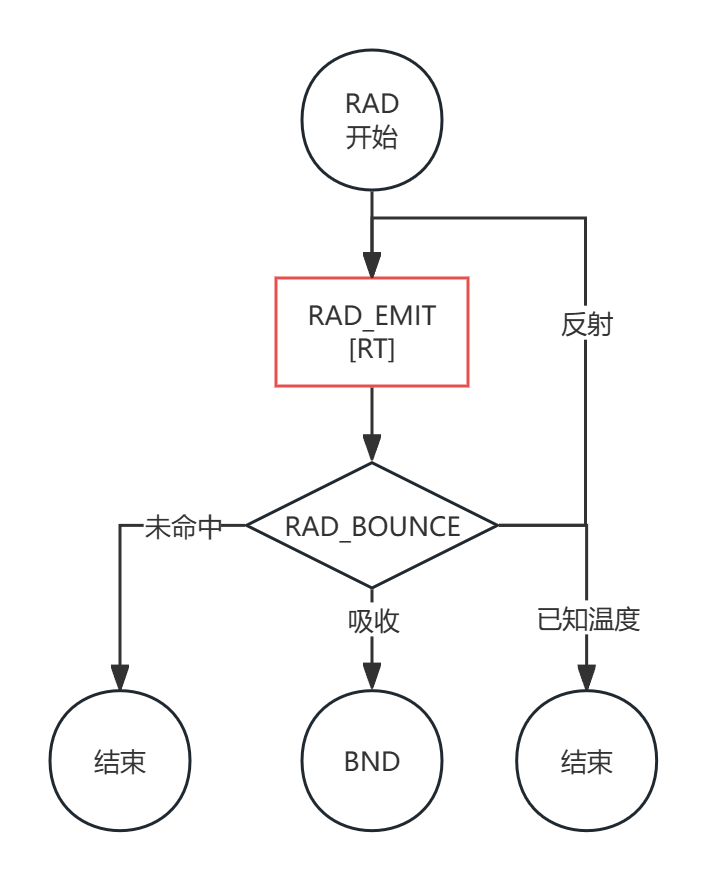
\includegraphics[width=0.5\textwidth]{Figures/FSM_RAD/FSM_RAD.png}
  \bicaption{RAD 辐射传播模块的状态转移图}{FSM state transition diagram of the RAD radiative transport module}
  \label{fig:fsm-rad}

  \small
  圆圈节点为模块入口/出口及终止条件，红色边框方形为含 RT 查询的挂起点，
  菱形为分支决策状态。路径从探测器或 BND 辐射出射进入 RAD，
  经余弦采样弹射循环，以 $\varepsilon$ 概率吸收（转入 BND）或射线逃逸终止。
\end{figure}

\subsubsection{固体传导模块（CND）：扩散方程驱动的球面随机游走}

路径经 BND 模块以传导概率 $P_\text{cond}$ 渗入固体内部后，传播机制从直线辐射切换为球面随机游走——对应图~\ref{fig:coupled_path} 中路径从 BND~1 事件后在 Solid~A 壁体中执行的 CND 折线步进段。球面随机游走求解固体内瞬态扩散方程\cite{batiCouplingConductionConvection2023}：
\begin{equation}
  \frac{\partial \theta_S}{\partial t} = \alpha \Delta \theta_S
  \label{eq:cnd-diffusion}
\end{equation}
其中 $\alpha = k/(\rho c)$ 为热扩散率，$\theta_S$ 为固体温度场。其蒙特卡洛求解由如下估计量驱动：
\begin{equation}
  \theta_S(\mathbf{x} - \delta\hat{n}) = E\bigl[\theta_S(\mathbf{x}_\text{WoS})\bigr]
  \label{eq:cnd-wos-estimator}
\end{equation}
即在固体边界面内侧 $\delta$-偏移处的温度，等于从该点出发的球面随机游走到达边界时温度的期望值。每步将游走粒子投射到球面上的随机位置，球半径由几何或物理参数确定；当粒子到达固体边界时，路径回到 BND 模块开始新一轮界面耦合分叉。实现中存在两种球面游走方案：

\textit{Walk-on-$\delta$-Sphere（$\delta$-球面游走）}使用固定步长参数 $\delta$ 替代最近面距离作为球面半径\cite{batiCouplingConductionConvection2023}。每步采样均匀球面方向 $\boldsymbol{\Omega}$，沿 $+\boldsymbol{\Omega}$ 和 $-\boldsymbol{\Omega}$ 两方向各追踪一条射线（RT 查询），取命中距离 $s^+$、$s^-$ 与 $\delta$ 的最小值作为实际步长：
\begin{equation}
  \tilde{\delta} = \min(\delta,\,s^+,\,s^-)
  \label{eq:cnd-ds-step}
\end{equation}
粒子跳至 $\mathbf{x} + \tilde{\delta}\,\boldsymbol{\Omega}$，随后以 ENC 查询验证新位置的腔体归属。若跳跃后位置进入 $\varepsilon$-壳层（$\tilde{\delta}$-球面吸附至边界），则路径转入 BND 模块——对应图~\ref{fig:coupled_path} 中 CND 游走段的三个出射分支（BND~2、BND~4、BND~5 分别命中固-流内表面、固-流外表面和固-固接触面）；否则进行瞬态时间回溯采样后继续下一步游走。每步产生 1 个 RT 查询（双向射线对批量提交为一次查询）和 1 个 ENC 查询（位置验证）。

\textit{Walk-on-Sphere（经典 WoS 游走）}以最近面投影距离（CP 查询）作为球面半径，在远离边界处收敛性更优（对数收敛 vs $\delta$-球的固定步长）。每步首先执行 CP 查询获取最近面距离 $d_\text{wos}$：若 $d_\text{wos} \leq \varepsilon_\text{shell}(\delta)$，粒子吸附至边界并转入 BND；否则在 $d_\text{wos}$ 半径球面上均匀采样跳跃方向。跳跃后执行第二次 CP 查询验证新位置的最近面距离（扩散位置合法性检查）：若验证失败（新位置处于几何非凸区域），以 RT 查询发射回退射线修正位置。每步产生 2 个 CP 查询（步长估计 $+$ 位置验证）和至多 1 个条件性 RT 查询（仅在验证失败时触发）。

两种方案在实现中并存，由场景参数控制选择策略。

\textit{瞬态时间回溯}嵌入上述两种游走方案每步循环的尾部。按指数分布采样向后时间跳跃 $T_{b,\text{cond}}$，其特征时间为：
\begin{equation}
  \tau_\text{cond} = \frac{\rho c \tilde{\delta}^2}{6k}
  \label{eq:cnd-tau}
\end{equation}
若时间倒退至仿真初始时刻 $t_I$，路径以已知初始温度终止——对应图~\ref{fig:coupled_path} 中的 Done(Time) 终止条件；否则继续下一步游走。此逻辑为确定性计算，不产生额外查询。

\textbf{模块出口}：CND 路径在游走步到达固体边界时转入 BND 模块。如图~\ref{fig:coupled_path} 所示，同一条传导游走路径因命中不同性质的边界面而触发截然不同的后续物理机制——BND~4（固-流外表面，辐射反弹或对流终止）、BND~2（固-流内表面，再发射穿越封闭腔体）、BND~5（固-固接触面，按导热系数比跨壁传导）——由 BND 模块统一处理。

\begin{figure}[htbp]
  \centering
  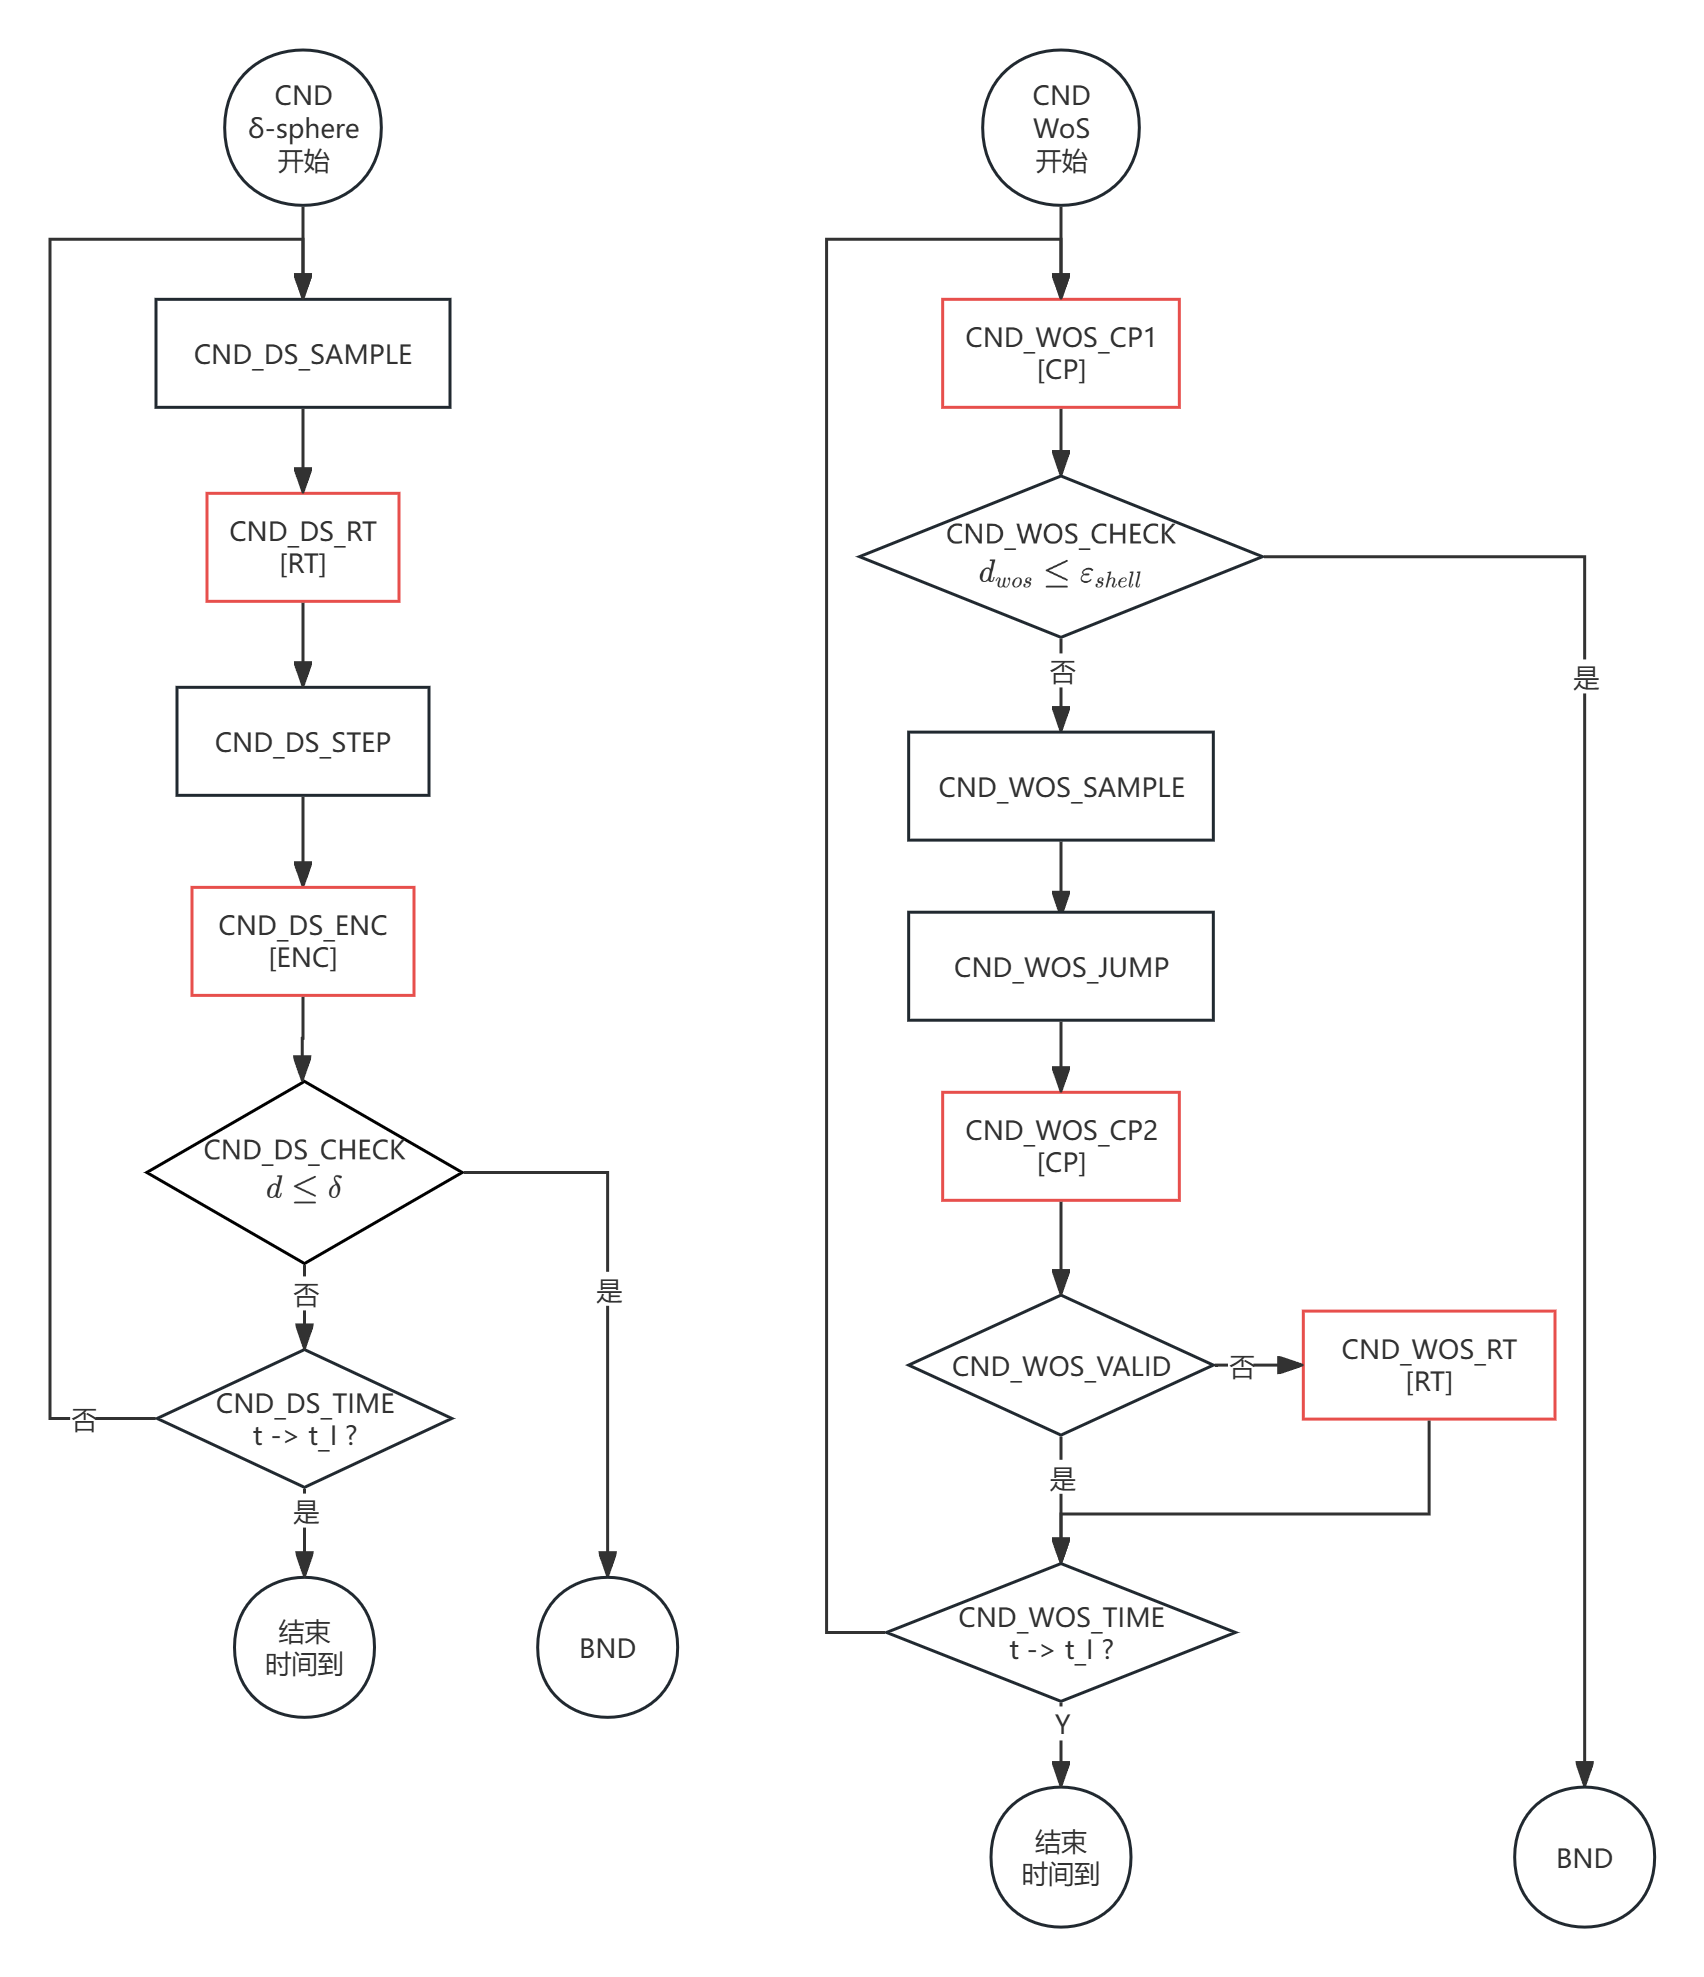
\includegraphics[width=0.7\textwidth]{Figures/FSM_CND/FSM_CND.png}
  \bicaption{CND 固体传导模块的状态转移图}{FSM state transition diagram of the CND solid conduction module}
  \label{fig:fsm-cnd}

  \small
  左侧为 $\delta$-球面游走方案（5 个状态），右侧为经典 WoS 游走方案（8 个状态），
  虚线方框分别包围两种游走方案。圆圈节点为模块入口/出口及终止条件，
  红色边框方形为含几何查询的挂起点（RT/CP/ENC），方形为线性计算状态，菱形为分支决策状态。
\end{figure}

\subsubsection{对流换热模块（CNV）：流体温度的边界采样}

当 BND 模块以对流概率 $P_\text{conv}$ 选择进入对流模式时，路径需获取当前封闭腔体的流体温度 $\theta_F$。\cite{batiCouplingConductionConvection2023} 框架假设完全混合流体（腔体内等温），$\theta_F$ 等于该腔体壁面固体温度的 $h(\mathbf{x})$-加权平均：
\begin{equation}
  \theta_F = E\bigl[\theta_S(\mathbf{X}_S)\bigr], \quad
  \mathbf{X}_S \sim \frac{h(\mathbf{x})}{\int_S h\,\mathrm{d}x}
  \label{eq:cnv-fluid-temp}
\end{equation}
蒙特卡洛采样将此期望估计为：在腔体边界面上按 $h(\mathbf{x})$ 成比例采样一个位置 $\mathbf{X}_S$，读取该处固体温度 $\theta_S(\mathbf{X}_S)$。若该位置温度已知（Dirichlet 边界），路径以 $\theta_F = \theta_S(\mathbf{X}_S)$ 终止——对应图~\ref{fig:coupled_path} 中 BND~4 出射分支的对流耗散终止 Done(Dissipation)；若温度未知，路径在 $\mathbf{X}_S$ 处再次触发 BND 事件，继续分叉求解。瞬态对流在腔体温度采样前引入指数分布的向后时间跳跃 $T_{b,\text{conv}}$，其特征时间为：
\begin{equation}
  \tau_\text{conv} = \frac{\rho c V}{hS}
  \label{eq:cnv-tau}
\end{equation}
其中 $V$ 为腔体体积，$S$ 为腔体壁面面积。若时间倒退至初始时刻 $t_I$，路径以已知初始流体温度终止。

CNV 模块的 FSM 结构包含 1 个 RT 查询，位于模块入口处的腔体几何边界探针射线——该射线确认路径所在腔体的几何边界范围，为后续按 $h(\mathbf{x})$ 采样壁面位置提供几何基础。边界采样本身为确定性计算，不产生额外查询。

\textbf{模块出口}：采样位置 $\mathbf{X}_S$ 处温度已知时路径终止；温度未知时回到 BND 模块继续耦合分叉。CNV 是全部传输模块中 FSM 结构最简洁的：4 个状态、1 个查询，反映了完全混合假设下对流模型的物理简洁性。

\begin{figure}[htbp]
  \centering
  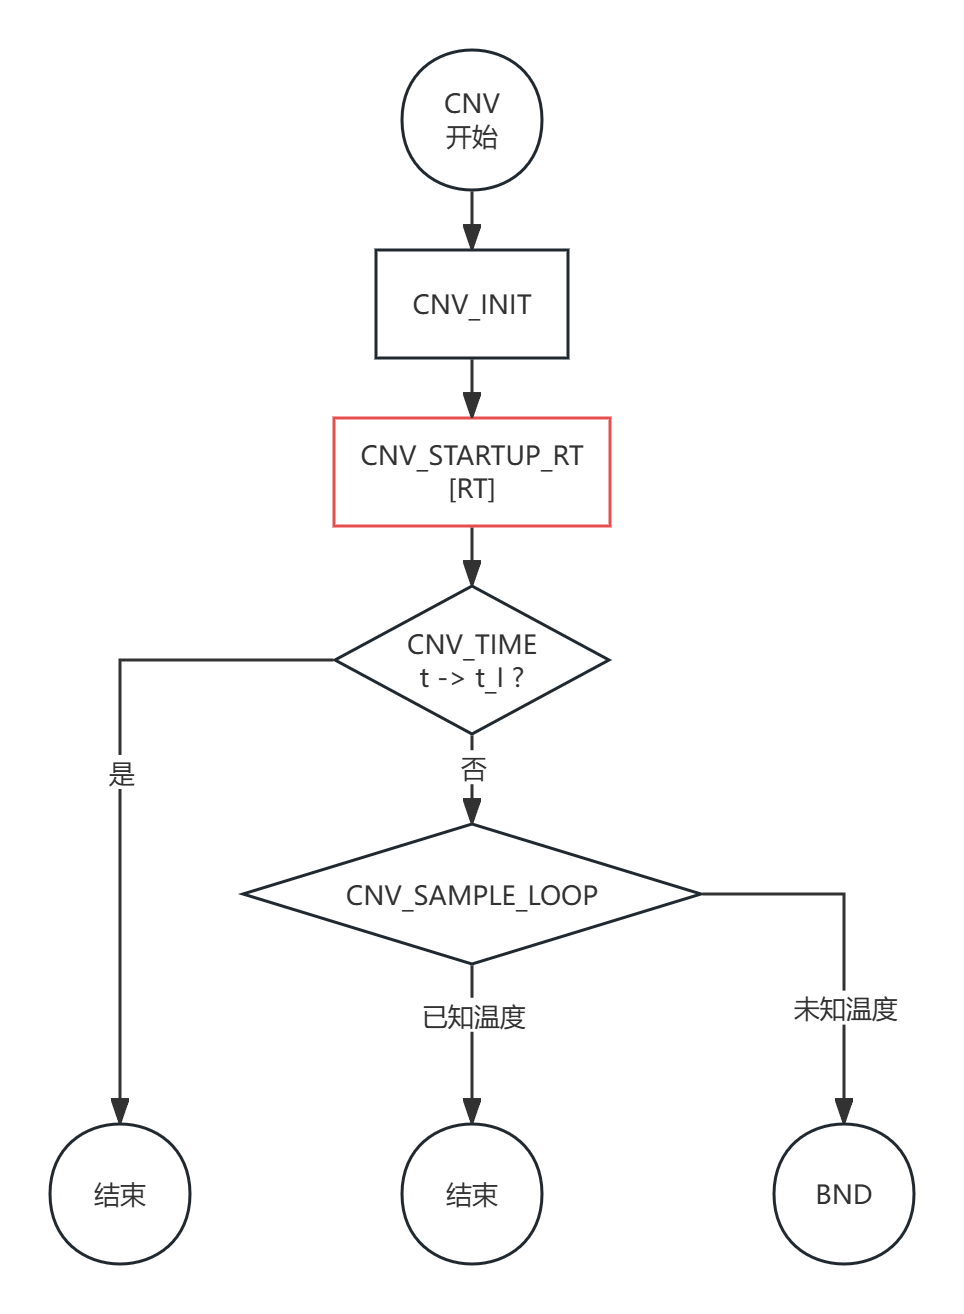
\includegraphics[width=0.4\textwidth]{Figures/FSM_CNV/FSM_CNV.png}
  \bicaption{CNV 对流换热模块的状态转移图}{FSM state transition diagram of the CNV convective heat transfer module}
  \label{fig:fsm-cnv}

  \small
  4 个状态，1 个 RT 查询。圆圈节点为模块入口/出口及终止条件，
  红色边框方形为含 RT 查询的挂起点，方形为线性计算状态，菱形为分支决策状态。
\end{figure}

\subsubsection{界面耦合模块（BND）：能量通量连续性驱动的多模态分叉}

界面耦合模块是整个 FSM 中状态数最多、分叉结构最复杂的部分。物理上，界面是辐射、传导、对流三种热传递模式交汇的核心节点——路径在界面处根据能量守恒的概率分叉决定进入何种传输模式继续前进。前文已分别介绍了 RAD、CND、CNV 三个传输模块的 FSM 结构，本段落展示 BND 如何作为三者的汇聚枢纽，在不同类型的界面处产生多模态分叉与状态回环。

BND 模块的物理总纲是界面能量守恒方程\cite{batiCouplingConductionConvection2023}：在任何固-流界面处，固体侧传导热通量等于流体侧对流通量与辐射通量之和：$\varphi_\text{cond}[\theta] = \varphi_\text{conv}[\theta] + \varphi_\text{rad}[L_\lambda]$。\ref{sec:coupled_framework} 已将此方程改写为概率期望形式（式~\eqref{eq:interface_temp}），界面温度由传导、对流、辐射三种模式的概率加权和表示，三个概率 $P_\text{cond}$、$P_\text{conv}$、$P_\text{rad}$ 由式~\eqref{eq:interface_probs} 给出。路径在界面处按上述概率随机选择进入 CND、CNV 或 RAD 模块——对应图~\ref{fig:coupled_path} 中各 BND 事件节点的扇形概率分支。

实际场景中界面类型多样，FSM 首先经过一个界面分发状态根据界面类型（固-流 / 固-固 / 外部环境）和温度可知性进行分流。下文按界面复杂度递增展开各子模块。

\textit{腔体归属查询（ENC）——界面参数查找的前置步骤}。固-流或固-固界面的物理参数（$\varepsilon$、$k$、$h$）绑定于封闭腔体（enclosure）。如图~\ref{fig:coupled_path} 所示的多层嵌套场景中，Solid~A 的外表面属于 Enc~A 而内表面属于 Enc~B，同一固体的不同面对应不同腔体参数集。路径到达界面后必须首先确定所属腔体才能查找正确的物理系数。腔体归属判定采用 6-ray 轴对齐投票方案：沿 $\pm x$、$\pm y$、$\pm z$ 六方向发射射线，根据命中面片的腔体标注投票确定归属；投票不一致时以随机方向回退射线补充。该过程产生 3 个 ENC 查询（BVH 最邻近定位、6-ray 主投票查询、歧义回退查询）。归属结果写入路径状态，后续全部 BND 子模块依赖此值读取正确物理参数。

\textit{固-流界面（SF）——三模态耦合与 null-collision}。当路径经传导游走到达固-流界面（对应图~\ref{fig:coupled_path} 中 BND~2、BND~4 类事件），或从辐射传播段被吸收后首次进入固体（BND~1），执行式~\eqref{eq:interface_temp} 的三模态概率分叉。FSM 子流程依次为：(1) $\delta$-重注入采样——沿界面法线内侧发射 RT 查询确定传导注入候选位置 $\mathbf{x} - \delta\hat{n}$；(2) 三概率 $P_\text{cond}/P_\text{conv}/P_\text{rad}$ 计算与模式调度——以 Russian Roulette 采样转移目标，传导分支进入 CND 模块、对流分支进入 CNV 模块。辐射分支的处理涉及式~\eqref{eq:null_collision} 所述的 null-collision 机制在界面耦合中的应用（\cite{batiCouplingConductionConvection2023} 6.3）：由于 $P_\text{rad}$ 含 $h_R = 4\sigma\varepsilon\theta_\text{ref}^3$，当参考温度 $\theta_\text{ref}$ 不准确时三概率之和偏离 1；为此设上界 $\hat{h}_R$ 使 $P_\text{rad}^\text{ub}$ 始终合法，采样辐射方向后发射 RT 查询获取子路径辐射温度 $\theta_R$，计算实际 $h_R$ 并以 $h_R/\hat{h}_R$ 概率接受（true collision），否则以 null collision 判定回到分叉状态重新采样。这一 null-collision 循环在 FSM 中对应 PENDING $\to$ 恢复 $\to$ 条件判断 $\to$ 回到 PENDING 的状态回边，与 RAD 弹射循环的 FSM 化方法完全同构。固-流界面子模块共产生 2 个 RT 查询（重注入射线 $+$ null-collision 辐射子路径射线）。图~\ref{fig:coupled_path} 中 BND~1 处的扇形分支即展示了 $P_\text{cond}$（渗入 Solid~A 启动 CND）、$P_\text{rad}$（漫反射回 Fluid~A 继续 RAD）和 $P_\text{conv}$（对流温度终止 $\theta_{F,A}$）三个出射方向。

\textit{PicardN 高阶迭代——递归子路径}。高温差场景中 $h_R$ 对温度强依赖，Picard-1 单轮线性化不足以收敛（\cite{batiCouplingConductionConvection2023} 6.3.3）。具体而言，$h_R = 4\sigma\varepsilon\theta_\text{ref}^3$ 是对 Stefan-Boltzmann 四次方律 $\sigma\varepsilon\theta^4$ 在参考温度 $\theta_\text{ref}$ 处的一阶 Taylor 线性化\cite{batiCouplingConductionConvection2023}。当界面两侧温差较小时，$\theta_\text{ref}$ 的选取误差对 $h_R$ 影响有限，Picard-1 的单轮 null-collision 采样即可收敛；而当温差显著时，$h_R \propto \theta_\text{ref}^3$ 的立方依赖使任何初始估计的偏差被放大，需通过多轮子路径采样逐步收紧 $\theta_\text{ref}$ 估计。PicardN 在界面处递归展开子路径树：每层展开至多 $N_\text{branch}$ 条完整耦合子路径（实现中 $\leq 6$ 条），递归深度可达 3 层。其 FSM 化的核心挑战在于将嵌套递归压平为显式栈：\texttt{path\_state} 中预分配固定深度递归栈（\texttt{path\_sfn\_data}，3 层，约 3.7\,KB/路径），以栈指针模拟展开与回退。子路径复用主 FSM 全部状态集（RAD/BND/CND/CNV）和挂起/恢复机制，不引入新的设计维度——仅增加栈管理字段。PicardN 的 6 个细粒度 FSM 状态及其查询与前述各模块的 FSM 化方法完全同构，不再逐一展开。

\textit{固-固界面（SS）——双侧导热注入}。当传导游走路径到达两个相邻固体子部件的接触面（对应图~\ref{fig:coupled_path} 中 BND~5: Solid~A $\leftrightarrow$ Solid~B），物理方程为式~\eqref{eq:ss_interface} 的传导通量连续性条件\cite{batiCouplingConductionConvection2023}。路径以 $P_{\text{cond},1}$ 概率选择注入固体 1 侧、以 $P_{\text{cond},2}$ 概率注入固体 2 侧的 $\delta$ 偏移处，继续传导游走。固-固界面不涉及辐射和对流模态（两侧均为不透明固体），分叉结构远简于固-流界面——仅为二元导热概率选择。FSM 子流程中，双侧各以 2 条射线（法线 $+$ 偏移修正）确定 $\delta$-注入候选位置（共 4 条 RT 批量提交），随后以 1 个 ENC 查询验证候选位置腔体归属，最终按概率选侧后进入 CND 模块。图~\ref{fig:coupled_path} 中 BND~5 注入 Solid~B 后路径继续游走，经 BND~6 最终终止于已知温度 Done(Known Temperature)。

\textit{外部环境边界（EXT）——净辐射通量子流程}。当路径到达与开放辐射环境交界的外部边界（而非封闭腔体内表面），需计算该表面从外部环境接收的净辐射通量（太阳直射 $+$ 天空漫射 $-$ 自发射），对应 \cite{batiCouplingConductionConvection2023} Eq.\,7 中 $\varphi_\text{rad}$ 的外部环境部分。蒙特卡洛子流程分三步有序执行：(1) 沿太阳方向发射阴影射线测试直射遮挡（RT 查询）；(2) 在天空半球按分布采样漫射方向（RT 查询）；(3) 对漫射命中方向发射遮挡验证射线（RT 查询）。三步严格有序，每步依赖前一步结果，须分配独立查询。该子模块共产生 3 个 RT 查询，是 BND 子模块中状态数最多的（8 个细粒度状态），反映了外部环境辐射场的多源（直射 $+$ 漫射）特征。

\begin{sidewaysfigure}
  \centering
  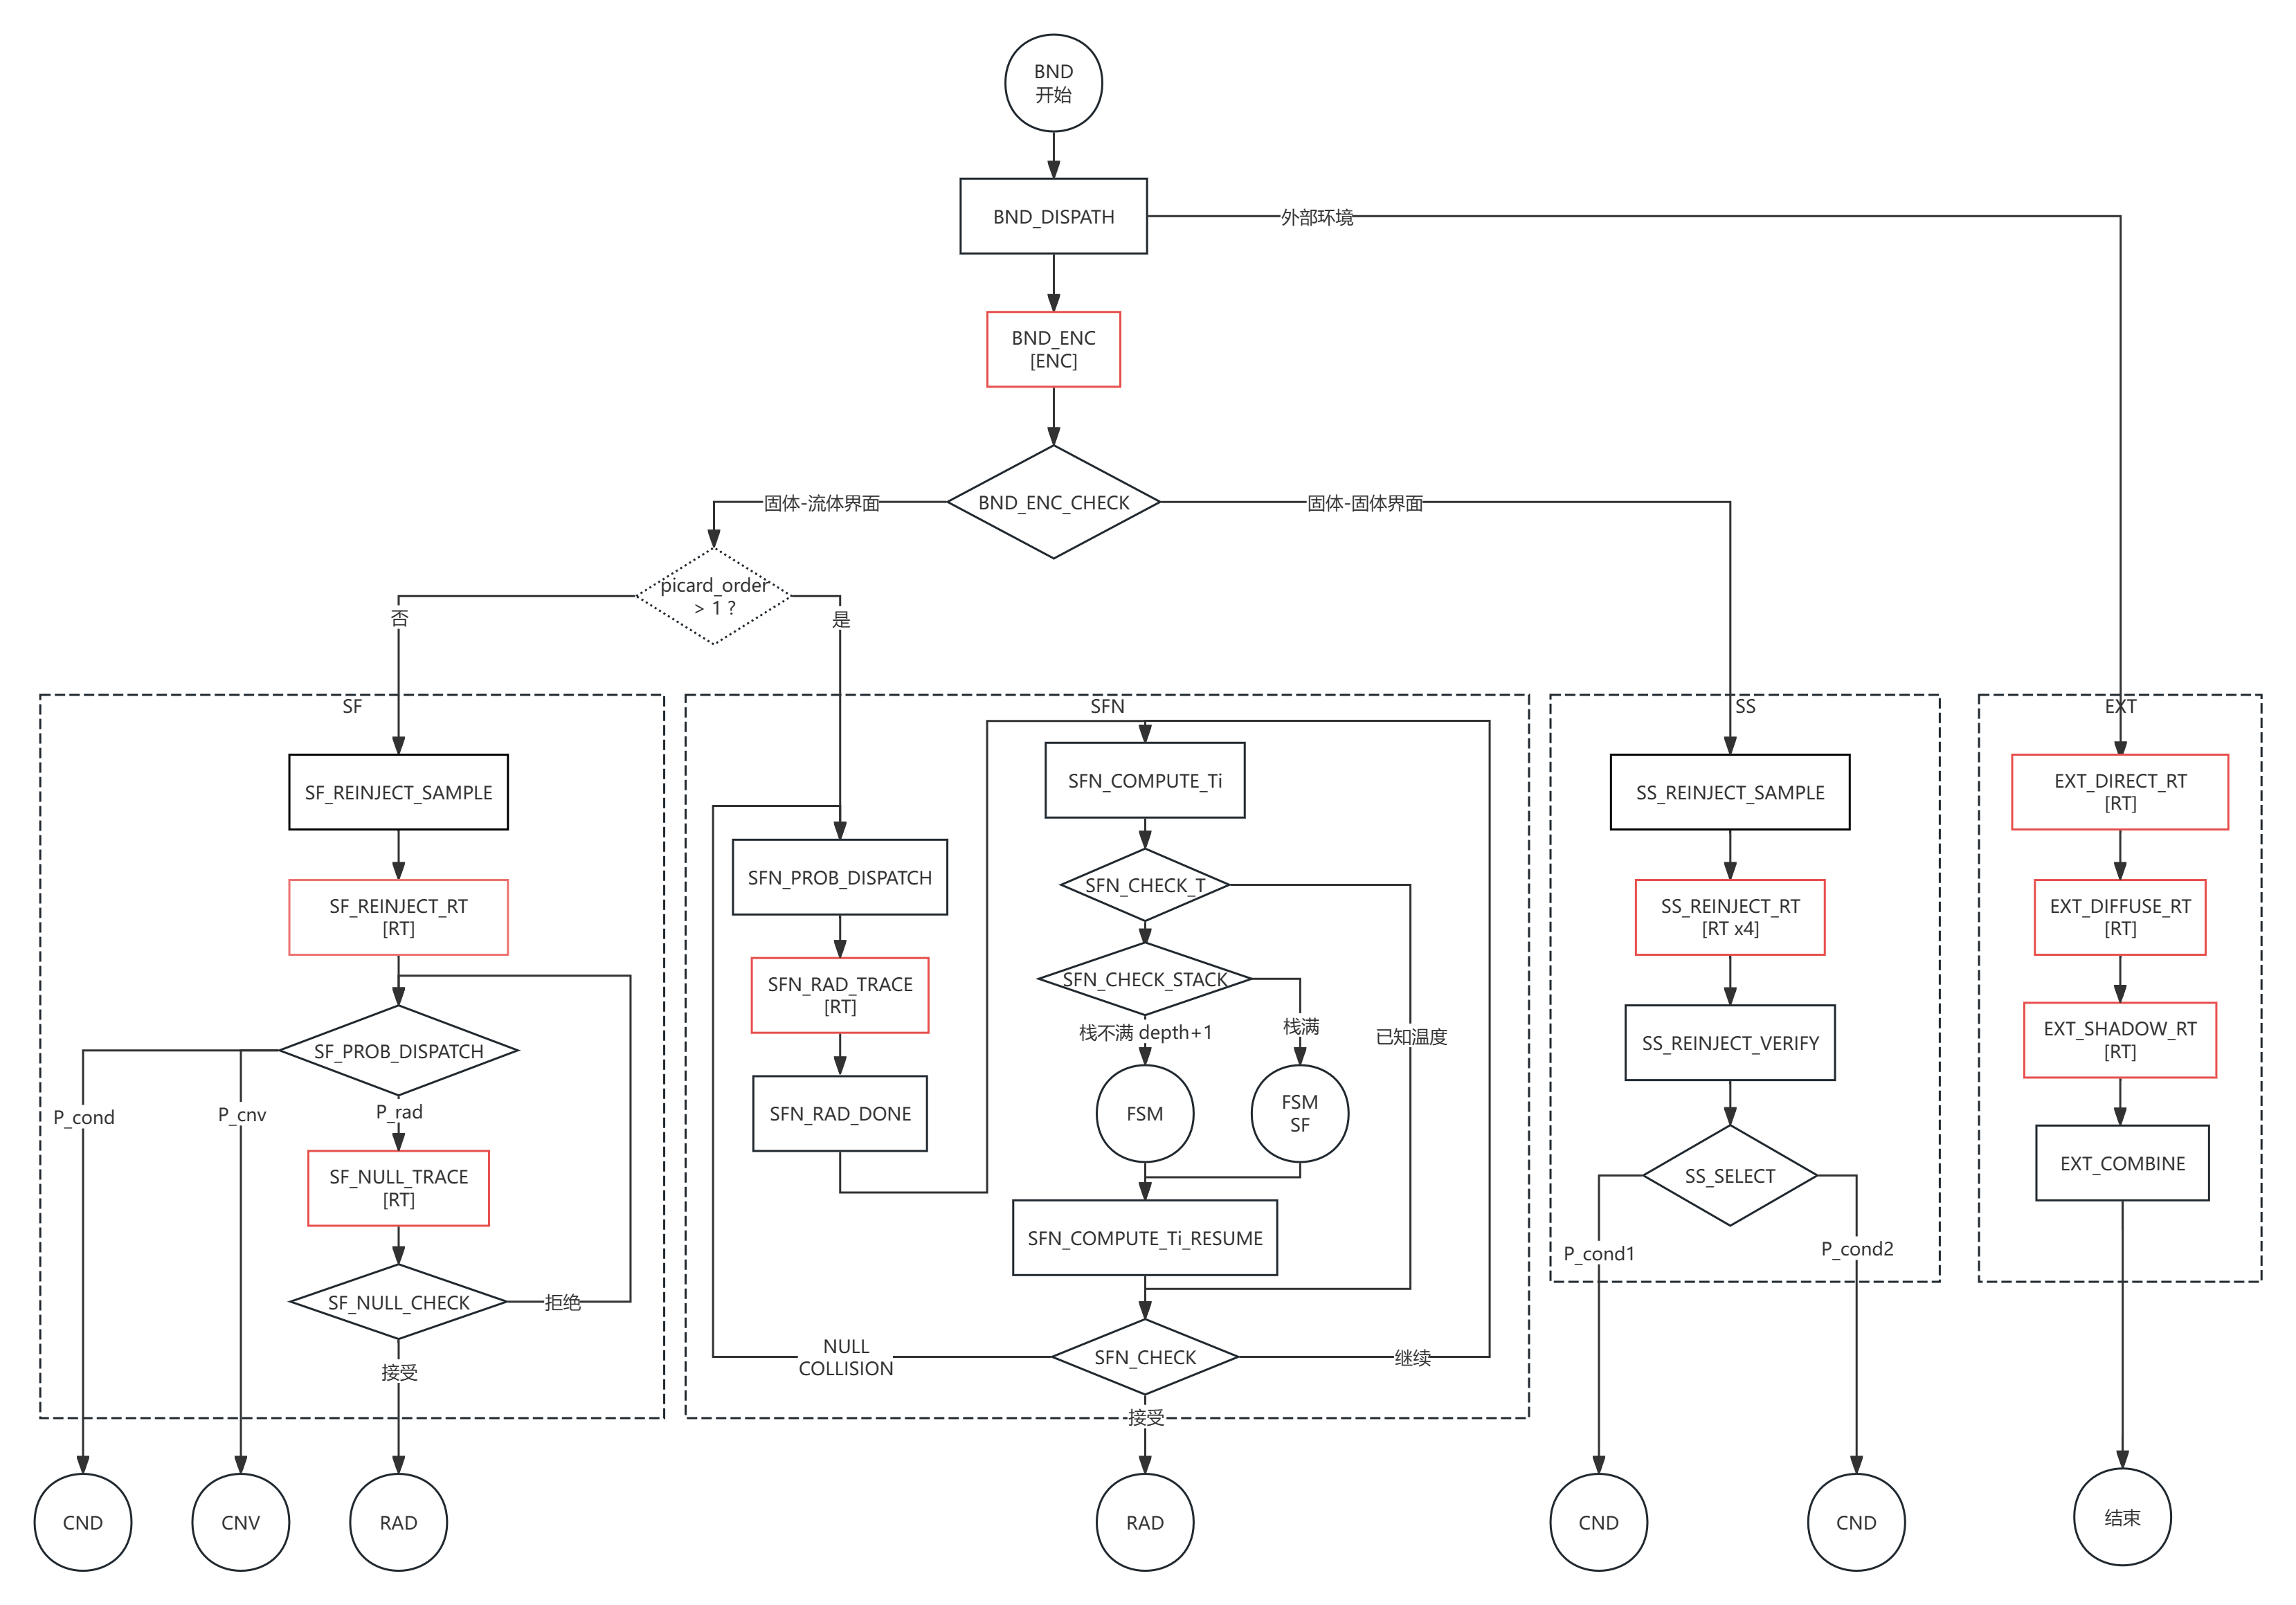
\includegraphics[width=0.9\textheight]{Figures/FSM_BND/FSM_BND.png}
  \bicaption{BND 界面耦合模块的分层状态转移图}{Hierarchical FSM state transition diagram of the BND interface coupling module}
  \label{fig:fsm-bnd}

  \small
  虚线方框包围 ENC、SF、SFN、SS、EXT 五个子模块。圆圈节点为模块入口/出口及终止条件，
  红色边框方形为含几何查询的挂起点（RT/ENC），方形为线性计算状态，菱形为分支决策状态。
  红色虚线回边标记 null-collision 循环，蓝色虚线标记 SFN 子路径迭代与栈递归。
\end{sidewaysfigure}

\subsubsection{完整 FSM 综合：模块组装与路径生命周期}

以上四个物理过程模块（RAD、CND、CNV）及其界面耦合枢纽（BND，含 ENC、SF、SFN、SS、EXT 五个子模块）共同构成耦合热输运路径的完整 FSM。组装方式由物理耦合关系唯一决定：路径从探测器出发经 RAD 弹射到达固体表面后进入 BND，BND 按界面类型和概率将路径分发至 CND（传导游走）、CNV（对流采样）或继续 RAD（辐射再发射）；CND 和 CNV 完成后再次返回 BND，形成 $\text{BND} \rightleftharpoons \text{CND/CNV/RAD}$ 的反复交替，直至路径终止于已知温度、初始时刻、环境辐射或俄罗斯轮盘赌截断四类条件之一。\cref{fig:coupled_path_meta} 已从粗粒度视角展示了这一模块间流转结构。

表~\ref{tab:module-summary} 汇总了各模块的状态数与几何查询需求。FSM 共包含 59 个细粒度状态，分属上述模块——其数量不是任意设计的结果，而是物理耦合复杂度的自然投影：3 种热传递模式 $\times$ 多种界面拓扑（固-流、固-固、外部环境）$\times$ 非线性耦合迭代（null-collision、PicardN）$\times$ 瞬态时间维度 $\times$ 实际几何复杂度（嵌套腔体），每种组合需要独立的查询通道。路径长度是场景物理参数（导热率、发射率、腔体尺度）的函数：最短可仅 2 步（RAD 直达 Dirichlet 边界终止），最长可达数千步（深 PicardN 递归 $+$ 长传导游走 $+$ 多次界面往返）。

\begin{table}[htbp]
  \centering
  \bicaption{各物理模块的 FSM 状态数与几何查询汇总}{Summary of FSM state counts and geometric queries by physical module}
  \label{tab:module-summary}
  \small
  \begin{tabular}{lccccc}
    \toprule
    物理模块 & 物理方程来源 & 状态数 & RT & ENC & CP \\
    \midrule
    RAD 辐射传播 & Bati Eq.\,6/19 & 2 & 1 & — & — \\
    BND-ENC 腔体归属 & 工程需求 & 3 & — & 3 & — \\
    BND-SF（Picard-1） & Bati Eq.\,23, 6.3 & 5 & 2 & dep & — \\
    BND-SFN（PicardN） & Bati 6.3.3 & 6 & 1+ & dep & — \\
    BND-SS 固-固界面 & Bati Eq.\,26 & 3 & 4 & dep & — \\
    BND-EXT 外部环境 & Bati Eq.\,7 & 8 & 3 & — & — \\
    CND-DS（$\delta$-Sphere） & Bati 4.2 & 5 & 2/步 & dep & — \\
    CND-WoS（Walk-on-Sphere） & Muller 1956 & 8 & 1 & — & 2 \\
    CNV 对流换热 & Bati Eq.\,28 & 4 & 1 & dep & — \\
    \midrule
    \textbf{合计} & — & \textbf{59} & \textbf{14 点} & \textbf{3 点} & \textbf{2 点} \\
    \bottomrule
  \end{tabular}

  \vspace{4pt}
  {\raggedright\footnotesize 注："dep"表示该模块依赖 ENC 查询结果（由 BND-ENC 子模块提供），但不直接产生 ENC 查询。"2/步"表示每个游走步产生 2 个 RT 查询。"1+"表示 PicardN 子路径复用主 FSM 各模块的 RT 查询，此处仅计入 PicardN 独有的辐射子路径射线查询。\par}
\end{table}

全部 19 个查询在本文的 Wavefront 实现中均为同构查询：RT、ENC、CP 三类查询均已后端化（第四章详述），共享同一批量提交接口。Wavefront 主循环无需区分查询类型，统一收集、统一提交、统一恢复，调度逻辑因此大幅简化。

值得说明的是，Wavefront 求解器下多条路径的随机数消耗顺序与递归求解器不同（递归求解器逐路径串行消耗，Wavefront 求解器按批次交错消耗），但各路径持有独立的 per-path 计数器基随机数生成器（CBRNG）密鑰，路径内部随机序列相互独立，消耗顺序的差异不影响蒙特卡洛估计量的统计无偏性。

\subsection{Wavefront 执行模型}
\label{subsec:wf-model}

3.3.1 将递归求解器等价改造为显式路径状态机（FSM），使单条路径在任意几何查询节点均可将完整中间状态持久化至外部结构体 \texttt{path\_state}，并在查询结果回填后无损恢复执行。至此，单条路径的可挂起性已经建立。

然而，可挂起性本身尚不构成批量化的充分条件。3.3.1 的 FSM 仅定义了单条路径的状态与转移规则；如何组织多条路径的并发调度——何时挂起、何时恢复、如何将分散在不同路径中的查询请求聚合为一个连续批次——尚未涉及。形式化地，设 $N$ 条路径同时处于活跃状态，每条路径在其生命周期内经历若干次几何查询挂起；在任一时刻，各路径处于 59 个 FSM 状态中的某一个，其中处于 \textsc{Pending} 状态的路径各自持有一条待执行的查询请求。问题可表述为：设计一种调度策略，使得 (1) 每轮迭代中所有 \textsc{Pending} 路径的查询请求被提取并聚合为连续缓冲区，统一提交至查询后端批量执行；(2) 执行结果回填至各路径的 \texttt{path\_state} 后，路径从挂起点恢复继续推进。

Laine 等人\cite{laineMegakernelsConsideredHarmful2013}在 GPU 路径追踪中提出的 Wavefront 执行模型为上述问题提供了成熟的架构范式（第 2.3 节已介绍其基本原理）。其核心思想是：以固定容量的路径池维护所有活跃路径的持久化状态，主循环在每轮迭代中完成查询结果回填、路径推进、已完成路径收割、空闲槽位补充与新查询请求收集，最终将该轮收集的全部查询批量提交至后端——如此往复，直至全部采样任务完成。本节将 Wavefront 范式应用于 3.3.1 的耦合热输运 FSM，设计具体的主循环结构。

\subsubsection{主循环结构}
Wavefront 求解器以固定容量的路径池（Path Pool）$\mathcal{P}[0..N_\text{pool}-1]$ 为核心数据结构，每个槽位存储一个 \texttt{path\_state} 结构体及其调度阶段标记 \texttt{phase}。\texttt{phase} 在调度层面取四种值：\textsc{Pending}（持有待执行查询，等待后端返回结果）、\textsc{Ready}（结果已回填，可继续推进 FSM）、\textsc{Done}（求解完成，待收割）、\textsc{Free}（空闲槽位）。主循环重复执行六个阶段直至全部像素采样完成，如算法~\ref{alg:wf-main-loop} 所示。

\begin{algorithm}
\caption{Wavefront 耦合热输运求解器主循环}
\label{alg:wf-main-loop}
\begin{algorithmic}[1]
\REQUIRE pixel task queue $\mathcal{Q}$, path pool $\mathcal{P}[0..N_\text{pool}-1]$, query backend $\mathcal{B}$
\ENSURE per-pixel temperature estimates $\hat{T}[\cdot]$
\WHILE{$\mathcal{Q}$ non-empty \textbf{or} $n_\text{active} > 0$}
  \STATE \textsc{DistributeResults}($\mathcal{P}$, $\mathcal{H}$) \COMMENT{Phase 1: 查询结果回填}
  \STATE \textsc{AdvancePaths}($\mathcal{P}$) \COMMENT{Phase 2: 路径状态推进}
  \STATE \textsc{HarvestDone}($\mathcal{P}$, $\hat{T}$) \COMMENT{Phase 3: 完成路径收割}
  \STATE \textsc{RefillSlots}($\mathcal{P}$, $\mathcal{Q}$) \COMMENT{Phase 4: 空闲槽位补充}
  \STATE \textsc{CollectQueries}($\mathcal{P}$, $\mathcal{R}$) \COMMENT{Phase 5: 查询请求提取}
  \STATE $\mathcal{B}$.\texttt{submit}($\mathcal{R}$) \COMMENT{Phase 6: 批量提交至查询后端}
\ENDWHILE
\end{algorithmic}
\end{algorithm}

该六阶段序列与本文实现的实际执行顺序一一对应，构成 Wavefront 求解器的最小调度循环——每个阶段承担单一职责，各阶段间以路径池 $\mathcal{P}$ 与请求/结果缓冲区（$\mathcal{R}$/$\mathcal{H}$）为共享数据进行隐式通信。以下算法~\ref{alg:wf-p1}--\ref{alg:wf-p5} 分别给出 Phase 1--5 各阶段的操作伪代码（Phase 6 \texttt{submit} 为后端接口调用，不展开）。

\textbf{Phase 1: \textsc{DistributeResults}}（算法~\ref{alg:wf-p1}）。将上轮后端返回的查询结果写回各路径。遍历路径池，对每条处于 \textsc{Pending} 状态的路径，将结果缓冲区 $\mathcal{H}$ 中对应条目的命中位置、法线、距离等字段写入其 \texttt{path\_state}，并将调度标记切换为 \textsc{Ready}，表示该路径可继续推进。

\begin{algorithm}[htbp]
\caption{\textsc{DistributeResults} — 查询结果回填}
\label{alg:wf-p1}
\begin{algorithmic}[1]
\FOR{$i = 0$ \textbf{to} $N_\text{pool}-1$}
  \IF{$\mathcal{P}[i].\texttt{phase} = \textsc{Pending}$}
    \STATE write $\mathcal{H}[\texttt{owner}^{-1}(i)]$ (hit position, normal, distance, $\ldots$) into $\mathcal{P}[i].\texttt{state}$
    \STATE $\mathcal{P}[i].\texttt{phase} \leftarrow \textsc{Ready}$
  \ENDIF
\ENDFOR
\end{algorithmic}
\end{algorithm}

\textbf{Phase 2: \textsc{AdvancePaths}}（算法~\ref{alg:wf-p2}）。推进所有 \textsc{Ready} 路径。对每条 \textsc{Ready} 路径反复调用 3.3.1 的 \texttt{fsm\_step}，执行 FSM 状态转移直至路径再次到达查询挂起点（\textsc{Pending}）或求解完成（\textsc{Done}）。两次挂起之间可能跨越多个 FSM 状态——例如从 BND 概率分叉到 CND WoS 步进再到下一挂起射线——均在此阶段内完成。

此处存在一个关键细节：3.3.1 的 PicardN 子模块通过显式递归栈将父路径"分裂"为子路径——子路径复用与普通路径完全同构的 FSM 状态集与推进/收割管线，这一同构性是 Wavefront 批量处理的内在要求。然而，当子路径完成求解到达 \textsc{Done} 时，若不加拦截，\textsc{HarvestDone} 将直接回收该槽位，连同父路径的递归栈帧一起被清除。为此，\textsc{AdvancePaths} 在每次 \texttt{fsm\_step} 后插入一项递归子路径拦截检查：若路径到达 \textsc{Done} 且其 PicardN 递归栈深度 $d_\text{sfn} > 0$（即当前路径是某层递归的子路径而非顶层路径），则将 FSM 状态重置为 \texttt{SFN\_COMPUTE\_Ti\_RESUME}、调度标记回退为 \textsc{Ready}，使推进循环继续执行。被拦截的路径随后在 FSM 内部完成栈弹出与父层上下文恢复，对求解器而言只需一行栈深度判断，全部递归复杂度被封装在 FSM 状态转移逻辑中。

\begin{algorithm}[htbp]
\caption{\textsc{AdvancePaths} — 路径状态推进}
\label{alg:wf-p2}
\begin{algorithmic}[1]
\FOR{$i = 0$ \textbf{to} $N_\text{pool}-1$}
  \IF{$\mathcal{P}[i].\texttt{phase} = \textsc{Ready}$}
    \REPEAT
      \STATE \texttt{fsm\_step}($\mathcal{P}[i]$) \COMMENT{执行一次 FSM 状态转移（3.3.1）}
      \IF{$\mathcal{P}[i].\texttt{phase} = \textsc{Done}$ \textbf{and} $\mathcal{P}[i].\texttt{state}.d_\text{sfn} > 0$}
        \STATE $\mathcal{P}[i].\texttt{state}.\texttt{fsm} \leftarrow \texttt{SFN\_COMPUTE\_Ti\_RESUME}$ \COMMENT{拦截递归子路径}
        \STATE $\mathcal{P}[i].\texttt{phase} \leftarrow \textsc{Ready}$ \COMMENT{继续推进而非收割}
      \ENDIF
    \UNTIL{$\mathcal{P}[i].\texttt{phase} \in \{\textsc{Pending}, \textsc{Done}\}$}
  \ENDIF
\ENDFOR
\end{algorithmic}
\end{algorithm}

\textbf{Phase 3: \textsc{HarvestDone}}（算法~\ref{alg:wf-p3}）。收割已完成路径。对每条 \textsc{Done} 路径，将其携带的估计值累加至对应像素的温度估计 $\hat{T}$，然后将槽位标记为 \textsc{Free}，供后续 \textsc{RefillSlots} 补入新路径。

\begin{algorithm}[htbp]
\caption{\textsc{HarvestDone} — 完成路径收割}
\label{alg:wf-p3}
\begin{algorithmic}[1]
\FOR{$i = 0$ \textbf{to} $N_\text{pool}-1$}
  \IF{$\mathcal{P}[i].\texttt{phase} = \textsc{Done}$}
    \STATE $\hat{T}[\mathcal{P}[i].\texttt{pixel}]$ += $\mathcal{P}[i].\texttt{value}$; \quad $n_\text{active} \leftarrow n_\text{active} - 1$
    \STATE $\mathcal{P}[i].\texttt{phase} \leftarrow \textsc{Free}$
  \ENDIF
\ENDFOR
\end{algorithmic}
\end{algorithm}

\textbf{Phase 4: \textsc{RefillSlots}}（算法~\ref{alg:wf-p4}）。从像素任务队列 $\mathcal{Q}$ 中取出新采样任务填入空闲槽位。每条新路径初始化探测器位置、初始方向与 CBRNG 密钥，并在 \texttt{state} 中准备初始查询（首条射线），\texttt{phase} 直接置为 \textsc{Pending}。

\begin{algorithm}[htbp]
\caption{\textsc{RefillSlots} — 空闲槽位补充}
\label{alg:wf-p4}
\begin{algorithmic}[1]
\FOR{$i = 0$ \textbf{to} $N_\text{pool}-1$}
  \IF{$\mathcal{P}[i].\texttt{phase} = \textsc{Free}$ \textbf{and} $\mathcal{Q}$ non-empty}
    \STATE $(\text{pixel}, \text{sample\_id}) \leftarrow \mathcal{Q}.\texttt{dequeue}()$
    \STATE initialize $\mathcal{P}[i]$: detector position, initial direction, CBRNG key
    \STATE prepare startup query (initial ray) in $\mathcal{P}[i].\texttt{state}$
    \STATE $\mathcal{P}[i].\texttt{phase} \leftarrow \textsc{Pending}$; \quad $n_\text{active} \leftarrow n_\text{active} + 1$
  \ENDIF
\ENDFOR
\end{algorithmic}
\end{algorithm}

\textbf{Phase 5: \textsc{CollectQueries}}（算法~\ref{alg:wf-p5}）。遍历路径池，从所有 \textsc{Pending} 路径的 \texttt{path\_state} 中提取查询参数（射线起点、方向、查询类型标识等），紧凑追加至请求缓冲区 $\mathcal{R}$，同时记录每条查询到其所属路径槽位的映射 \texttt{owner}，供下轮 \textsc{DistributeResults} 定位回填目标。由于 3.3.1 的同构查询设计——RT、ENC、CP 三类查询共享同一后端提交接口——\textsc{CollectQueries} 无需按查询类型分流，统一追加即可。

\begin{algorithm}[htbp]
\caption{\textsc{CollectQueries} — 查询请求提取}
\label{alg:wf-p5}
\begin{algorithmic}[1]
\STATE $n_\text{queries} \leftarrow 0$
\FOR{$i = 0$ \textbf{to} $N_\text{pool}-1$}
  \IF{$\mathcal{P}[i].\texttt{phase} = \textsc{Pending}$}
    \STATE extract query type, ray origin, direction from $\mathcal{P}[i].\texttt{state}$
    \STATE $\mathcal{R}[n_\text{queries}] \leftarrow$ query; \quad $\texttt{owner}[n_\text{queries}] \leftarrow i$
    \STATE $n_\text{queries} \leftarrow n_\text{queries} + 1$
  \ENDIF
\ENDFOR
\end{algorithmic}
\end{algorithm}

各阶段对路径 \texttt{phase} 标记的操作构成确定性的状态流转环：\textsc{DistributeResults} 将 \textsc{Pending} 转为 \textsc{Ready}（结果已写回，允许推进）；\textsc{AdvancePaths} 将 \textsc{Ready} 推进至 \textsc{Pending}（产生新查询）或 \textsc{Done}（求解完成）；\textsc{HarvestDone} 将 \textsc{Done} 释放为 \textsc{Free}；\textsc{RefillSlots} 将 \textsc{Free} 初始化为 \textsc{Pending}（含初始查询）；\textsc{CollectQueries} 仅读取 \textsc{Pending} 路径的查询参数，不改变状态。因此，任一路径在其生命周期内按如下序列流转：
\begin{equation*}
\textsc{Free} \xrightarrow{\text{Refill}} \textsc{Pending} \xrightarrow{\text{Distribute}} \textsc{Ready} \xrightarrow{\text{Advance}} \cdots \xrightarrow{\text{Advance}} \textsc{Done} \xrightarrow{\text{Harvest}} \textsc{Free}
\end{equation*}

首轮迭代时 \textsc{DistributeResults} 和 \textsc{AdvancePaths} 因无 \textsc{Pending}/\textsc{Ready} 路径而自然空转，\textsc{RefillSlots} 填充路径池后交由 \textsc{CollectQueries} 收集初始查询，调度循环自此进入稳态。

路径池容量 $N_\text{pool}$ 在求解器启动时确定，全部 \texttt{path\_state} 结构体以连续数组分配。路径池运行宏观上分为两个阶段：\textit{填充阶段}——像素任务队列 $\mathcal{Q}$ 尚有未分配任务，每轮 \textsc{RefillSlots} 将空闲槽填满新路径，路径池填充率接近 100\%，提交的查询规模保持在峰值附近；\textit{收尾阶段}——$\mathcal{Q}$ 已空，\textsc{RefillSlots} 无新路径补入，活跃数逐轮递减直至清零。

\textbf{路径优先遍历优化}。算法~\ref{alg:wf-p1}--\ref{alg:wf-p3} 及算法~\ref{alg:wf-p5} 各独立遍历路径池一次（四次线性扫描）。在实现中，本文将此四次扫描融合为单次路径优先（path-centered）遍历——对每条路径连续执行 distribute$\to$advance$\to$harvest/collect 完整序列后才移向下一条路径。该融合确保同一条路径的 \texttt{path\_state} 在被首次加载到缓存行后，后续全部操作均在该缓存行驻留期间完成，显著改善缓存局部性。路径优先遍历不改变各阶段的语义——仅将四次独立扫描合并为一趟，是纯实现层面的优化。

综上，Wavefront 主循环在 \textsc{Collect} 与 \textsc{Distribute} 两阶段之间形成了明确的批量请求/批量响应接口边界：\textsc{Collect} 产出请求缓冲区 $\mathcal{R}$（经 \texttt{submit} 提交至后端），\textsc{Distribute} 消费后端返回的结果缓冲区 $\mathcal{H}$——查询的具体执行过程对状态推进逻辑完全透明。这条接口边界将求解器的计算职责一分为二：状态推进（Phase 1--5，逻辑密集、缓存敏感）与批量查询执行（Phase 6 \texttt{submit}，高吞吐、并发密集）。两类计算需求的分离是 3.3.3 异构架构设计的直接出发点。

\subsection{CPU-GPU 混合执行架构}
\label{subsec:hybrid-arch}

3.3.2 的 Wavefront 主循环在 \textsc{Collect} 与 \textsc{Distribute} 之间形成了明确的批量接口边界，将求解器的计算职责分为两个角色：角色 A（状态推进）——运行 distribute、advance、harvest、refill、collect 等逻辑（算法~\ref{alg:wf-p1}--\ref{alg:wf-p5}），频繁随机读写 \texttt{path\_state} 数组；角色 B（批量查询执行）——接受请求缓冲区 $\mathcal{R}$ 中数万条查询请求，返回结果缓冲区 $\mathcal{H}$。两角色在数据流上的解耦是 Wavefront 执行模型的直接产物。本节在此基础上，根据两类计算的硬件资源需求特征，设计 CPU-GPU 混合执行架构与异步调度机制。

\subsubsection{架构选型与接口设计}

3.3.2 的 Wavefront 批量接口将求解器的计算职责分离为状态推进（角色 A：算法~\ref{alg:wf-p1}--\ref{alg:wf-p5}）与批量查询执行（角色 B：\texttt{submit}）两类独立任务，这两类任务天然适合由 CPU-GPU 异构架构分别承担：角色 A 由 CPU 执行，角色 B 由 GPU 执行。两角色通过一个设备无关的查询接口层交互，接口层定义三个操作原语：
\begin{itemize}[nosep]
  \item \texttt{submit($\mathcal{R}$, $n$)}：将 $n$ 条查询请求提交至后端，异步语义——调用立即返回，后端在独立执行上下文中并行处理。
  \item \texttt{sync()}：等待最近一次 \texttt{submit} 对应的后端计算完成。
  \item \texttt{retrieve($\mathcal{H}$, $n$)}：将 $n$ 条查询结果从后端传输至结果缓冲区 $\mathcal{H}$。
\end{itemize}
接口层将后端的具体执行设备对角色 A 完全屏蔽。请求缓冲区 $\mathcal{R}$ 与结果缓冲区 $\mathcal{H}$ 采用结构体数组（SoA）布局，以连续内存存储同类查询字段，便于后端以对齐方式批量读取。

\textbf{本文选用的后端实例化}：角色 B 由 NVIDIA GPU 承担——三类几何查询的 GPU 批量管线设计（RT 光追管线、CP 最近面投影管线、ENC 腔体归属管线）将在第四章独立展开。本节以下内容聚焦于两角色在异步通信下的调度架构设计。

\subsubsection{Path-Centered 合并遍历}
\label{subsubsec:merge-pass}

\ref{subsec:wf-model} 将角色 A 的单轮工作描述为五个顺序 Phase——Distribute、Advance、Harvest、Refill、Collect——每个 Phase 各自遍历路径池数组。然而在实际落地时，路径池规模为 16\,384\textasciitilde 32\,768 条路径，每条 \texttt{path\_state} 约 3\textasciitilde 4\,KB；整个路径池工作集达 50\textasciitilde 128\,MB，远超典型 CPU 的 LLC 容量（16\textasciitilde 32\,MB）。若各 Phase 依次独立扫描路径池数组，则每轮产生多次完整遍历，每次遍历均将上一 Phase 的热缓存行逐出 LLC，导致大量 LLC miss 开销。

为消除这一缓存压力，实现将四个逐路径 Phase 合并为一次 path-centered 遍历（merged pass）。概念上，循环组织从
\begin{center}
\begin{minipage}{0.42\textwidth}
\begin{algorithmic}[0]
\FOR{\textbf{each} phase $p$ \textbf{in} \{1..5\}}
  \FOR{\textbf{each} path \textbf{in} pool}
    \STATE $p$(path)
  \ENDFOR
\ENDFOR
\end{algorithmic}
\end{minipage}%
\hfill$\Longrightarrow$\hfill%
\begin{minipage}{0.42\textwidth}
\begin{algorithmic}[0]
\FOR{\textbf{each} path \textbf{in} pool}
  \STATE Distribute(path)
  \STATE Advance(path)
  \STATE Harvest(path)
  \STATE Collect(path)
\ENDFOR
\STATE Compact(pool) ; Refill(pool)
\end{algorithmic}
\end{minipage}
\end{center}
右侧结构使每条路径的 \texttt{path\_state} 仅加载一次 L1 缓存行，四个操作在该缓存行仍热时依次完成：
Distribute 写回上一轮光追/CP/ENC 结果并触发对应 step 函数；
Advance（cascade）在无新查询需求的路径上执行内循环推进直至状态机进入 \texttt{needs\_ray}、\texttt{PATH\_DONE} 或 \texttt{PATH\_ERROR}；
Collect 将需要查询的路径的请求写入线程局部缓冲区；
Harvest 收集已完成路径的估计器结果。
遍历结束后，线程局部缓冲区合并至全局请求缓冲区 $\mathcal{R}$。

Refill（空槽填充）与 Compact（活跃索引重建）因涉及路径池级全局状态变更，无法逐路径嵌入，故保留为合并遍历之后的独立阶段。最终角色 A 的单轮 View 处理降为三步：
\[
  \texttt{merged\_pass}(\mathcal{V}) \;\to\; \texttt{compact}(\mathcal{V}) \;\to\; \texttt{refill}(\mathcal{V}) \;\to\; \texttt{submit}(\mathcal{V}.\mathcal{R})
\]
相比原始五次独立扫描，合并遍历将路径池的完整遍历次数从五次降至一次，大幅减少 LLC 换入换出开销，是缩短 $T_A$ 的关键手段。

\subsubsection{单池时序瓶颈与双池 Ping-Pong 调度}

在算法~\ref{alg:wf-main-loop} 的单路径池循环中，角色 A 完成本轮 collect 并调用 \texttt{submit} 后，必须阻塞于 \texttt{sync()} 等待后端返回结果，此间角色 A 完全空闲；反之，角色 A 执行 Phase 1--5 期间后端亦无任务可执行。将两角色的单轮耗时分别记为 $T_A$（Phase 1--5：distribute + advance + harvest + refill + collect）和 $T_B$（submit + 后端执行 + retrieve），则单池循环的每轮墙钟时间为 $T_A + T_B$，两角色的有效利用率均不超过 $\max(T_A, T_B) / (T_A + T_B)$。当角色 B 为 GPU 后端时，$T_B$ 包含 PCIe 传输（H2D + D2H）与 GPU kernel 执行，均可通过异步 DMA 和非阻塞 launch 在独立硬件上下文中执行而不占用 CPU 计算资源——但在单池架构下，角色 A 无法利用这一异步能力，因为当前路径池的状态已提交至后端、结果尚未返回，角色 A 没有可处理的路径。图~\ref{fig:timing-single-pool} 展示了这一串行瓶颈。

\begin{figure}[htbp]
  \centering
  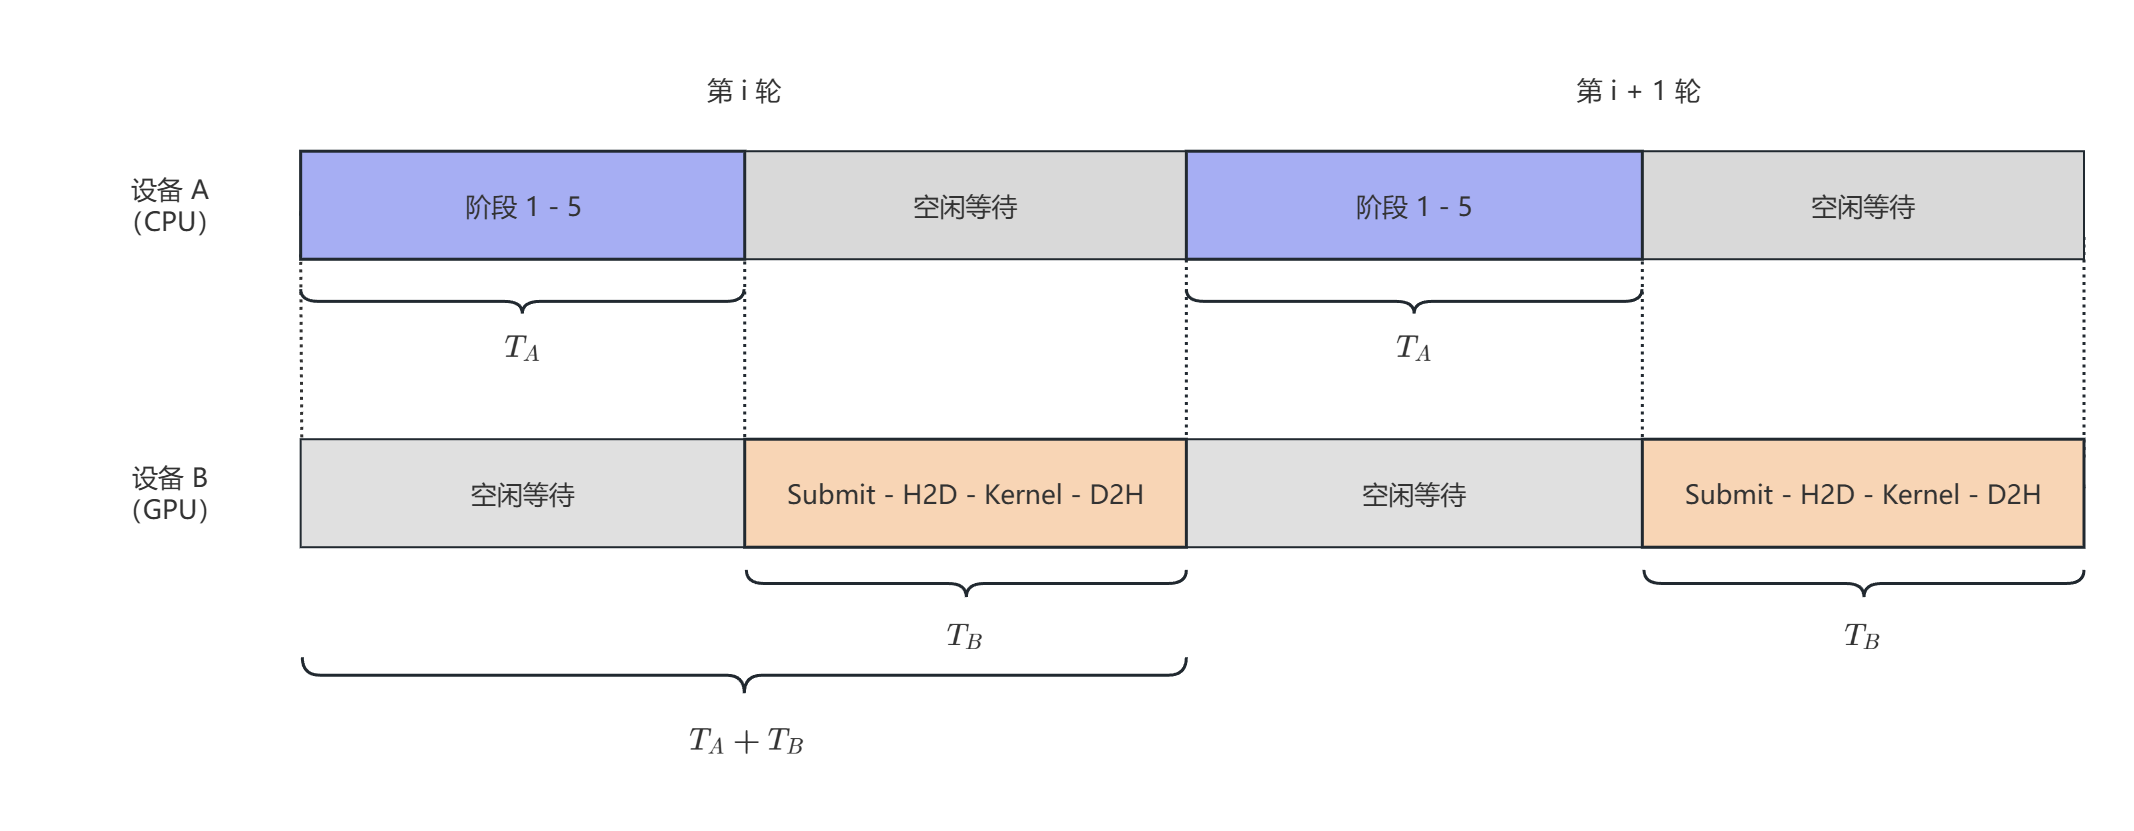
\includegraphics[width=0.90\textwidth]{Figures/Timing_SinglePool/SinglePoolTimeline.png}
  \bicaption{单路径池架构执行时序}{Execution timeline of the single-pool architecture}
  \label{fig:timing-single-pool}

  \small
  上行为角色 A（CPU）时间轴，下行为角色 B（GPU 后端）时间轴。
  角色 A 的工作段（蓝色，Phase 1--5）与角色 B 的工作段（橙色，Submit--H2D--Kernel--D2H）严格串行：角色 A 执行 Phase 1--5 期间角色 B 处于 Idle Waiting（灰色），角色 B 执行批量查询期间角色 A 同样处于 Idle Waiting（灰色）。
  大括号标注各段耗时：$T_A$（角色 A 单轮耗时）、$T_B$（角色 B 单轮耗时），每轮墙钟时间为 $T_A + T_B$，两角色从不同时工作。
\end{figure}

\textbf{双池 Ping-Pong 调度}通过将路径池拆分为两个半独立视图（View $\alpha$、View $\beta$），使两角色的执行时间窗口交错重叠，从根本上消除上述空闲间隙。算法~\ref{alg:pingpong} 展示了双池主循环的核心结构。

\begin{algorithm}
\caption{双池 Ping-Pong 主循环}
\label{alg:pingpong}
\begin{algorithmic}[1]
\REQUIRE path pool views $\mathcal{V}_\alpha$, $\mathcal{V}_\beta$; query backend $\mathcal{B}$
\STATE current $\leftarrow \alpha$; \quad pending $\leftarrow \beta$
\STATE $\mathcal{B}$.\texttt{submit}($\mathcal{V}_\beta.\mathcal{R}$) \COMMENT{bootstrap: pre-submit View $\beta$}
\WHILE{任务未全部完成}
  \STATE $\mathcal{B}$.\texttt{sync}() \COMMENT{等待 View $pending$ 的后端查询完成}
  \STATE $\mathcal{B}$.\texttt{retrieve}($\mathcal{V}_{pending}.\mathcal{H}$) \COMMENT{结果回传至 View $pending$}
  \STATE Phase 1--5 on View $current$ \COMMENT{角色 A: distribute$\to$advance$\to$harvest$\to$refill$\to$collect}
  \STATE $\mathcal{B}$.\texttt{submit}($\mathcal{V}_{current}.\mathcal{R}$) \COMMENT{角色 B 开始执行 View $current$ 批次}
  \STATE swap(current, pending) \COMMENT{视图切换}
\ENDWHILE
\end{algorithmic}
\end{algorithm}

双池调度的时序关键在于：角色 A 处理 View $current$ 的 Phase 1--5（distribute$\to$advance$\to$harvest$\to$refill$\to$collect）时段，与角色 B 执行 View $pending$ 的批量查询在时间上完全重叠。具体而言：角色 A 提交 View $\alpha$ 的批次后立即切换至处理 View $\beta$ 的上一轮结果，此时后端在独立硬件上下文中并行执行 View $\alpha$ 的查询；待角色 A 处理完 View $\beta$ 并提交其新批次时，View $\alpha$ 的结果已就绪，角色 A 可立即取回并切换回处理 View $\alpha$。图~\ref{fig:timing-pingpong} 展示了这一交错执行时序。

\begin{figure}[htbp]
  \centering
  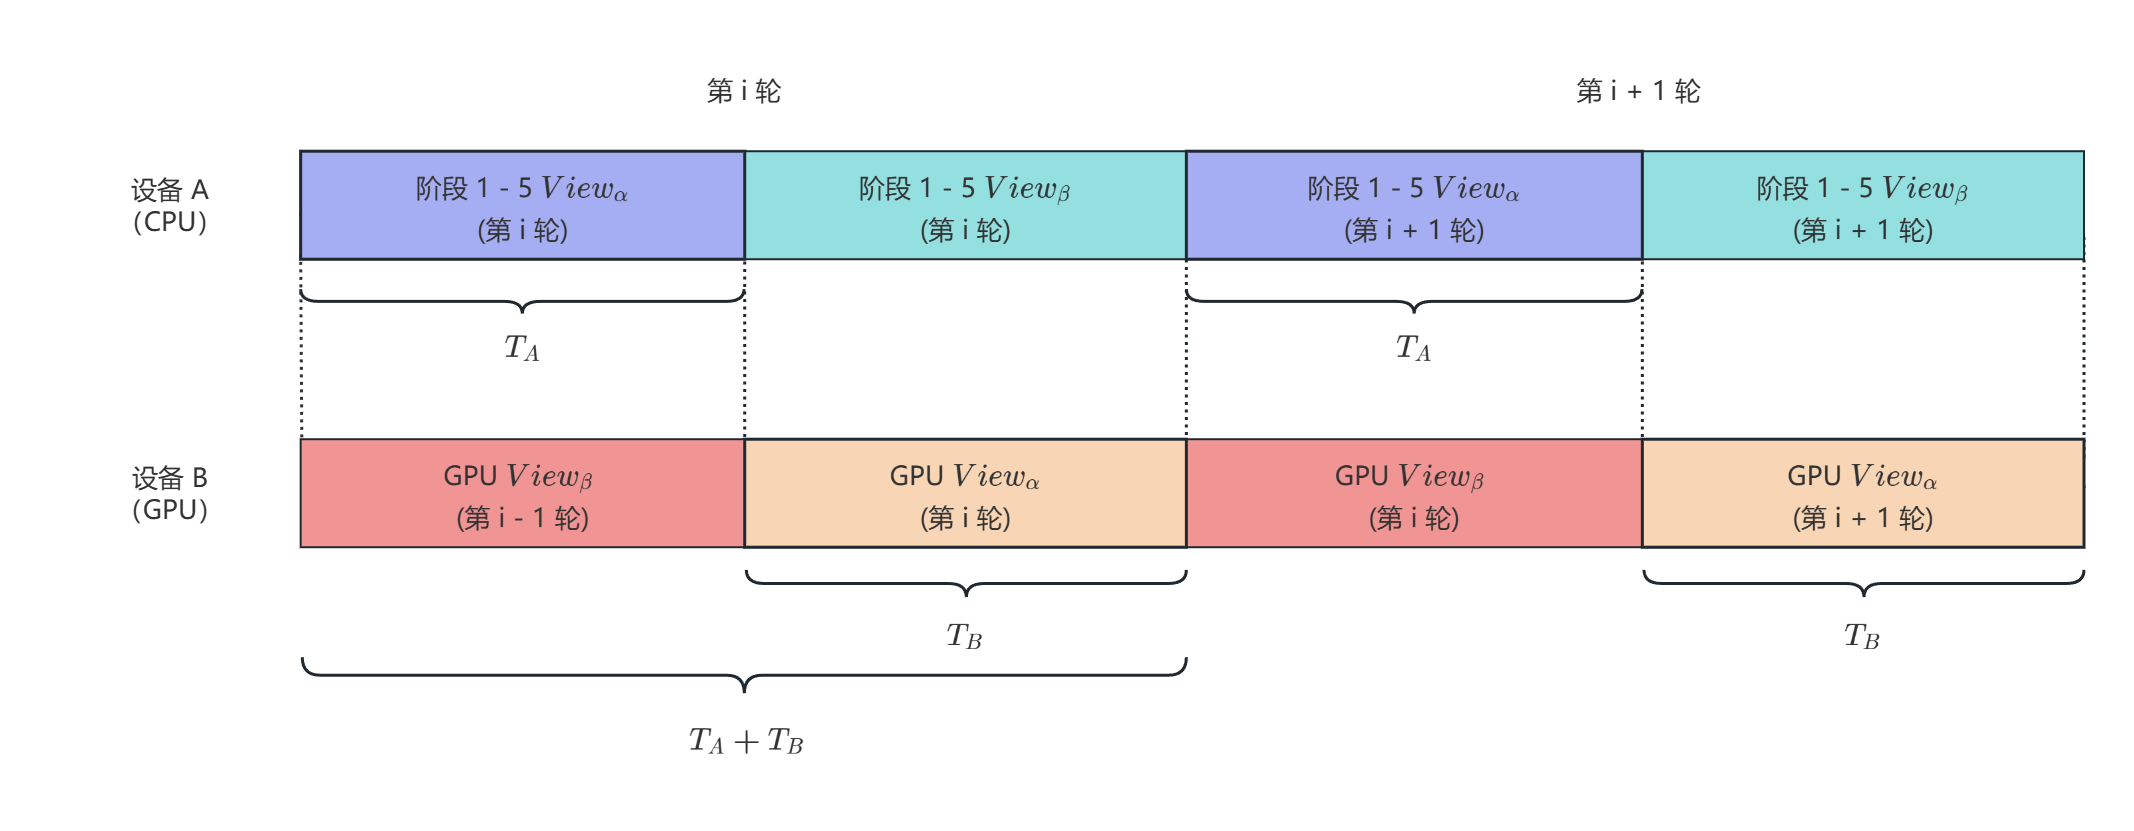
\includegraphics[width=0.90\textwidth]{Figures/Timing_PingPong/DualPoolTimeline.png}
  \bicaption{双池 Ping-Pong 调度执行时序}{Execution timeline of dual-pool Ping-Pong scheduling}
  \label{fig:timing-pingpong}

  \small
  上行为角色 A（CPU）时间轴，下行为角色 B（GPU 后端）时间轴。
  角色 A 的工作段以颜色区分两个 View：View $\alpha$（紫色）与 View $\beta$（青色）交替排列；角色 B 对应地以粉色（GPU View $\beta$）与橙色（GPU View $\alpha$）交替执行批量查询，每段标注所属 Round 编号。
  与图~\ref{fig:timing-single-pool} 对比可见：对任意单个 View 而言，其完整处理周期仍为 $T_A + T_B$（延迟未缩短）；但图~\ref{fig:timing-single-pool} 中两角色的空闲间隙（灰色段）现已被另一 View 的计算任务填充——延迟被隐藏而非缩短。
  大括号标注各段耗时：$T_A$（角色 A 单轮耗时）、$T_B$（角色 B 单轮耗时）；系统吞吐量从单池的每 $(T_A + T_B)$ 完成一个 View 提升至每 $\max(T_A, T_B)$ 完成一个 View，在 $T_A \approx T_B$ 条件下可达约两倍吞吐量。
\end{figure}

需要强调的是，双池调度并不缩短单个 View 的处理延迟——每个 View 从 distribute 到 retrieve 完成仍需经历完整的 $T_A + T_B$。其核心机制在于延迟隐藏：通过引入第二个 View 填充原本闲置的设备时间，使系统吞吐量从单池的每 $(T_A + T_B)$ 完成一个 View 提升至每 $\max(T_A, T_B)$ 完成一个 View。当两角色耗时匹配（$T_A \approx T_B$）时，吞吐量接近单池的两倍。不可避免的同步等待仅发生在两角色耗时不平衡时——当 $T_B > T_A$ 时，角色 A 在 \texttt{sync()} 处等待后端完成；当 $T_A > T_B$ 时，后端在完成本批次后等待角色 A 提交下一批。3.4 的性能分析将报告实测吞吐量提升。

当角色 B 由 GPU 承担时，$T_B$ 进一步分解为三个可与角色 A 部分重叠的子阶段：请求上行传输（H2D，由非阻塞 DMA 执行）、GPU kernel 计算（RT/CP/ENC 三类查询在各自独立的 compute stream 上并行调度，三条流之间无数据依赖）、结果下行传输（D2H，同样由非阻塞 DMA 执行）。H2D 和 D2H 均通过异步 DMA 实现，不占用角色 A 的 CPU 计算资源——这使得即便在 PCIe 带宽受限的条件下，数据传输延迟也可被角色 A 的计算时间所隐藏。

\section{结果与性能评估}

\subsection{实验设置}

本节描述实验环境与评估方法。实验在配备 Intel Core i9-13900K 处理器（8 Performance + 16 Efficiency 核心，P-core 睿频 5.8 GHz）和 NVIDIA GeForce RTX 4090 显卡（Ada Lovelace 架构，16384 CUDA Cores，128 第三代 RT Cores）的工作站上进行，搭配 64 GB DDR5 内存，操作系统为 Windows 11。软件工具链包括 MSVC 19.41（Visual Studio 2022 17.11）、CUDA 12.6、OptiX 8.0 和 NVIDIA 驱动 560.94。Windows 电源计划设置为"高性能"模式以禁用 CPU 频率降档，GPU Boost 保持默认启用（自适应频率）。

每组性能配置运行 3 次，取墙钟时间中位数作为报告值。

测试场景选用 porous（多孔泡沫）场景，包含 13{,}010 个三角面片和多个封闭腔体。该场景材质涵盖高发射率辐射表面（RAD/BND 过程密集）和内部导热体（CND 过程密集），是覆盖四种物理过程的典型多模态耦合热输运场景。主测试配置为 $320 \times 320$ 分辨率、32 SPP（Samples Per Pixel，每像素采样数）；高精度统计验证配置为 $512 \times 512$ 分辨率、128 SPP。

表~\ref{tab:comparison-setup} 给出两组对比方案的配置。两方案使用相同的物理模型和蒙特卡洛采样算法，差异仅存在于求解器架构（递归 vs Wavefront）与几何查询后端（Embree vs OptiX）。

\begin{table}[htbp]
  \centering
  \bicaption{性能对比实验方案}{Experimental configuration for performance comparison}
  \label{tab:comparison-setup}
  \small
  \begin{tabular}{llll}
    \toprule
    方案 & 求解器架构 & 几何查询后端 & 代码目录 \\
    \midrule
    Baseline & 递归求解器 & Embree (\texttt{rtcIntersect1}) & \texttt{stardis-cpu} \\
    Ours     & CPU Wavefront & OptiX GPU 批量查询 & \texttt{stardis-oxs3d} \\
    \bottomrule
  \end{tabular}
\end{table}

评估从两个维度展开：\emph{物理一致性}验证 Wavefront 架构改造不引入系统性物理偏差；\emph{端到端性能}以墙钟时间和加速比 $S = T_{\text{Baseline}} / T_{\text{Ours}}$ 衡量，并通过控制 CPU 线程数和路径池容量分析性能瓶颈。

\subsection{一致性验证}

由于递归求解器与 Wavefront 求解器的随机数消耗顺序不同——递归求解器逐路径串行消耗，Wavefront 求解器按批次中断恢复后交错消耗——两者对同一像素产生的路径样本序列必然不同。逐像素差异反映的是随机数种子差异，而非算法偏差，因此不能解读为``误差''。本节从物理过程解析解对比和端到端统计等价性检验两个互补维度验证一致性。

\subsubsection{物理过程一致性验证}

构造覆盖物理复杂度阶梯的 13 个验证场景，每个场景具有解析解或高精度数值参考解，总计 282 个有效数据点（GPU 134 + CPU 148），$3\sigma$ 通过率均为 100\%。整体验证集如表~\ref{tab:consistency-suite} 所示，覆盖 Poisson 稳态、瞬态扩散、对流换热、辐射边界、多材料界面、嵌套几何、多域多物理耦合等核心物理机制。性能与端到端统计等价性评估则在 porous 场景上展开，其在单一案例中同时激活辐射—传导—对流三类耦合过程，是受控对比的代表性载体。

\begin{table}[htbp]
  \centering
  \bicaption{物理一致性验证场景一览}{Physical consistency verification suite}
  \label{tab:consistency-suite}
  \small
  \begin{tabular}{lll}
    \toprule
    物理场景 & 参考解类型 & 主要验证功能 \\
    \midrule
    平板稳态导热 + 均匀体源 & 一维 Poisson 倒抛物线 & 空间扩散与体源采样 \\
    双材料拼接 + 接触热阻 & 分段线性折线族 & 多材料异质性 \\
    内嵌同材料透明体 & 嵌套介质单点 & 介质嵌套处理 \\
    边界通量内部剖面 & 已知边界通量解 & 边界通量传播 \\
    三线性温度场批量探针 & 三线性插值场 & 批量探针一致性 \\
    多阶 Picard 导热—辐射耦合 & 高阶 Picard 迭代参考 & 高阶非线性求解 \\
    立方体六面对流换热瞬态 & 集总指数衰减 & 时间积分 + 对流边界 \\
    非均匀对流换热 & 空间非均匀对流解 & 边界空间不均匀性 \\
    扩散方程制造解法 & $\sin\!\times\!\exp$ 时空解 & 完整 PDE 时空一致性 \\
    流体—固体—大气多域瞬态 & 高精度数值参考 & 多域多物理耦合 \\
    外部太阳源辐射 & 外源辐射解 & 远场通量注入 \\
    漫射辐照 & 漫射边界解 & 漫射辐射边界 \\
    嵌套包壳体积功率 & 嵌套体积源解 & 复杂嵌套 + 体源耦合 \\
    \bottomrule
  \end{tabular}
\end{table}

以下逐实验介绍物理背景、理论公式和验证结果。Wavefront 求解器与递归求解器分别求解各场景后，将估计值 $E$ 与参考值 $T_{\mathrm{ref}}$ 对比，采用蒙特卡洛 $3\sigma$ 准则判定通过：

\begin{equation}
  \label{eq:3sigma-criterion}
  \sigma = \frac{|E - T_{\mathrm{ref}}|}{\mathrm{SE}} \leq 3
\end{equation}

\noindent 其中 $\mathrm{SE}$ 为蒙特卡洛标准误差。若估计器无偏且服从正态分布，$\sigma \leq 3$ 对应 99.7\% 置信区间。

\paragraph{实验一：稳态导热——体积热源倒抛物线}

平板两面固定温度 $T_0 = 320$~K，板内均匀体积热源功率密度 $P = 10$~W/m$^3$，导热系数 $\lambda = 0.1$~W/(m$\cdot$K)。稳态温度分布满足 Poisson 方程 $\nabla^2 T = -P/\lambda$ 的一维特解：

\begin{equation}
  \label{eq:a2-parabola}
  T(x) = \frac{P}{2\lambda}\left(\frac{1}{4} - \left(x - \frac{1}{2}\right)^2\right) + T_0
\end{equation}

\noindent 形成对称倒抛物线，中心温度最高 $T_{\max} = P/(8\lambda) + T_0 = 332.5$~K，两端等于边界温度 320~K。沿 $x$ 轴等间距布置 11 个探针，GPU 与 CPU 各 11 个数据点均精确落在解析抛物线上（图~\ref{fig:consistency-a2}），$\sigma$ 最大值分别为 2.691 和 2.676，全部通过 $3\sigma$ 检验（GPU 11/11，CPU 11/11）。

\begin{figure}[htbp]
  \centering
  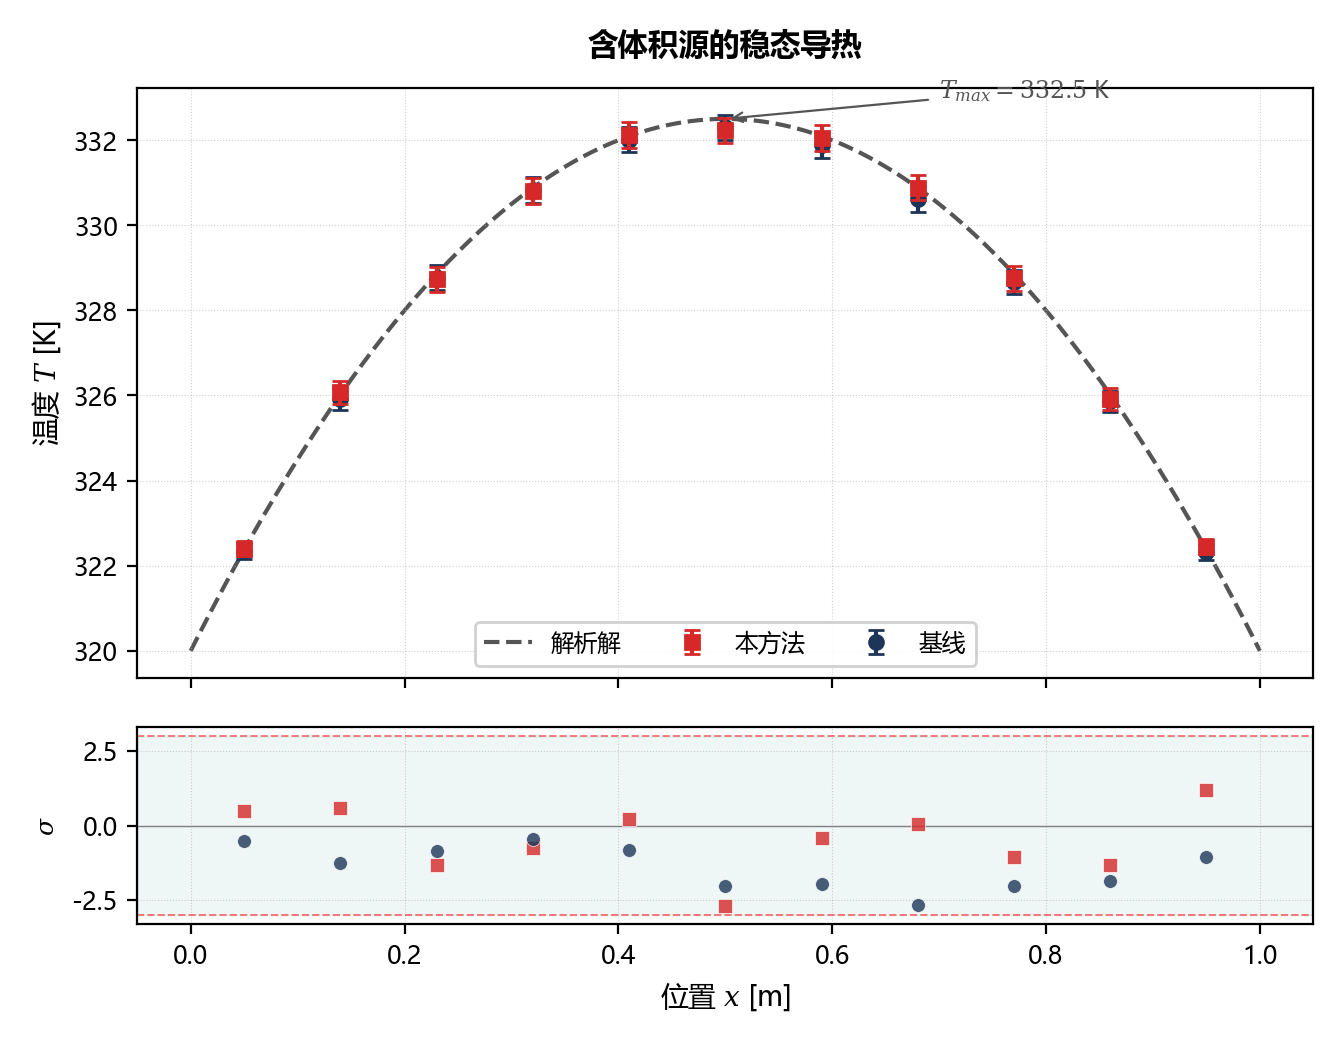
\includegraphics[width=0.85\textwidth]{Figures/Consistency/fig1_a2_parabola.png}
  \bicaption{稳态导热体积热源验证}{Steady-state volumetric heat source verification}
  \label{fig:consistency-a2}

  \small
  Wavefront 求解器（红色方块）与递归求解器（蓝色圆点）均精确复现倒抛物线解析解（灰色虚线），下方面板显示标准化偏差 $\sigma$ 均在 $\pm 3$ 以内。
\end{figure}

\paragraph{实验二：多材料界面——接触热阻折线族}

两种导热系数不同的材料（$\lambda_1 = 0.1$，$\lambda_2 = 0.2$~W/(m$\cdot$K)）拼接于 $x_0 = 3$~m 处，总长 $L = 4$~m，左端 $T_0 = 0$~K，右端 $T_L = 100$~K。界面接触热阻 $R$~[m$^2\cdot$K/W] 引入温度跳跃。稳态热流密度为

\begin{equation}
  \label{eq:a3-heatflux}
  q = \frac{T_L - T_0}{x_0/\lambda_1 + R + (L - x_0)/\lambda_2}
\end{equation}

\noindent 两侧温度分布均为线性：左侧 $T(x) = T_0 + (q/\lambda_1)\,x$，右侧 $T(x) = T_L - (q/\lambda_2)(L-x)$，界面温度跳跃 $\Delta T = q R$。5 个 $R$ 值（0.01, 0.1, 1, 10, 100）形成扇形展开的分段折线族——$R$ 越大，界面跳跃越大，曲线越平缓。GPU 以 5 组 $R$ 值系统扫描（40 个数据点），CPU 以随机 $R$ 采样（16 个数据点）从两个互补角度验证，全部通过 $3\sigma$ 检验（图~\ref{fig:consistency-a3}）。

\begin{figure}[htbp]
  \centering
  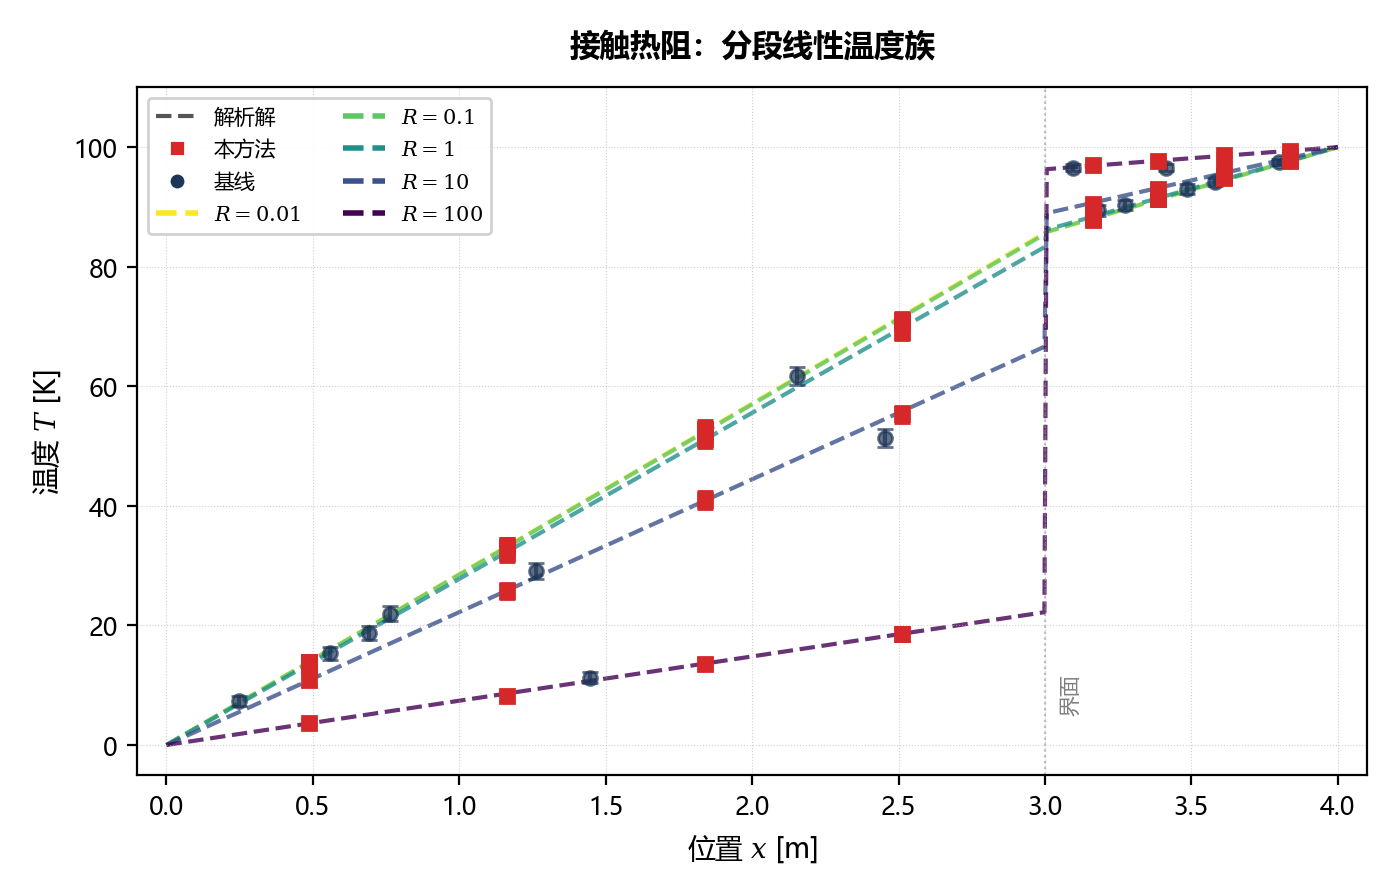
\includegraphics[width=0.85\textwidth]{Figures/Consistency/fig2_a3_contact_resistance.png}
  \bicaption{多材料接触热阻验证}{Multi-material contact resistance verification}
  \label{fig:consistency-a3}

  \small
  5 组 $R$ 值形成扇形折线族，GPU 40 个探针（红色方块）排列于各自对应折线上，CPU 16 个随机探针（蓝色圆点）散布于折线族中，均在 $3\sigma$ 区间内。
\end{figure}

\paragraph{实验三：对流换热瞬态——指数衰减}

立方体固体初始温度 $T_0 = 280$~K，六面暴露于均匀流体温度 $T_\infty = 325$~K，对流换热系数 $H$。集总参数模型（Biot 数 $\ll 1$）给出精确的指数趋近解：

\begin{equation}
  \label{eq:d1-exponential}
  T(t) = T_0\, e^{-\nu t} + T_\infty\left(1 - e^{-\nu t}\right)
\end{equation}

\noindent 其中衰减率 $\nu = 6H/(\rho c_p) = 1.2$~s$^{-1}$（六面均匀对流），时间常数 $\tau = 1/\nu \approx 0.83$~s。这是牛顿冷却定律最直观的时域表现——温度从 280~K 指数升温，渐近趋于 325~K。图~\ref{fig:consistency-d1} 展示了 4 个瞬态时刻和稳态极限处的验证结果，GPU（9/9）与 CPU（5/5）全部通过 $3\sigma$ 检验，精确复现了指数衰减动力学。稳态区间 GPU 5 个不同空间位置探针均给出 $E \approx 325.0$~K，验证了集总参数模型``稳态温度与空间位置无关''的物理预测。

\begin{figure}[htbp]
  \centering
  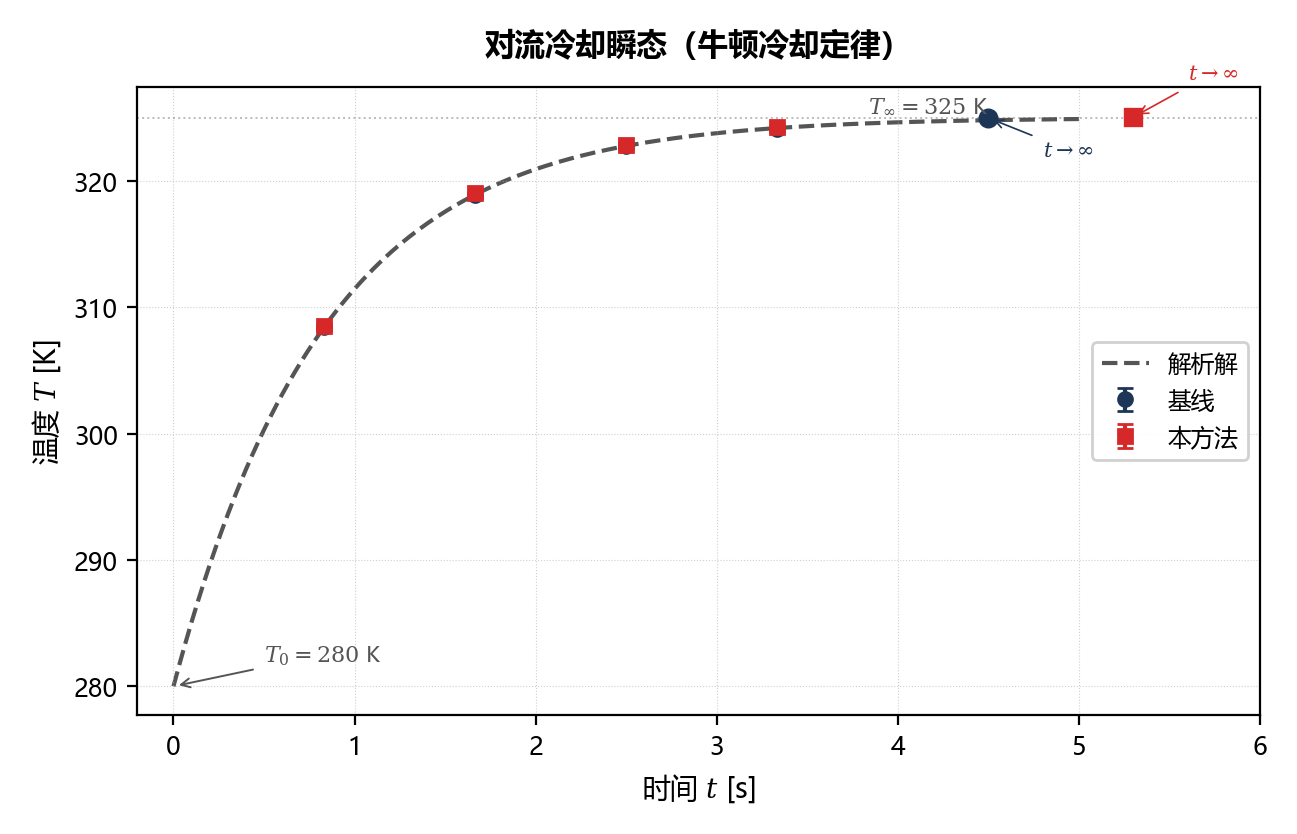
\includegraphics[width=0.85\textwidth]{Figures/Consistency/fig3_d1_convection.png}
  \bicaption{对流换热瞬态验证}{Transient convective heat transfer verification}
  \label{fig:consistency-d1}

  \small
  Wavefront 求解器（红色方块）与递归求解器（蓝色圆点）均精确复现牛顿冷却定律的指数衰减解析解（灰色虚线），渐近趋于流体温度 $T_\infty = 325$~K。
\end{figure}

\paragraph{实验四：扩散方程精确解——$\sin \times \exp$}

采用制造解法（Method of Manufactured Solutions）：在超形体几何体上预设解析温度场作为 Dirichlet 边界条件，由 MC 求解器反算内部温度后与预设解对比。解析解为稳态调和多项式与瞬态正弦本征模的叠加：

\begin{equation}
  \label{eq:e3-sinexp}
  T(x,y,z,t) = \frac{1}{\lambda}\left[B_1(x^3 z - 3xy^2 z) + B_2 \sin\frac{\pi x}{4}\sin\frac{\pi y}{4}\sin\frac{\pi z}{4}\cdot e^{-\alpha k^2 t}\right]
\end{equation}

\noindent 其中 $B_1 = 10$，$B_2 = 1000$，热扩散系数 $\alpha = \lambda/(\rho c_p) = 0.002$~m$^2$/s，$k^2 = 3(\pi/4)^2$，时间常数 $\tau = 1/(\alpha k^2) \approx 270$~s。图~\ref{fig:consistency-sinexp} 以双子图展示验证结果：左图固定空间点 $(0.2, 0.3, 0.4)$ 的温度随时间的指数衰减（对数时间轴，0.5\textasciitilde1000~s），右图固定时刻 $t = 5$~s 的温度沿 $x$ 轴的正弦空间分布。GPU（23/23）与 CPU（24/24）数据点均精确落在解析曲线上，同时验证了空间本征模式和时间积分的正确性。

\begin{figure}[htbp]
  \centering
  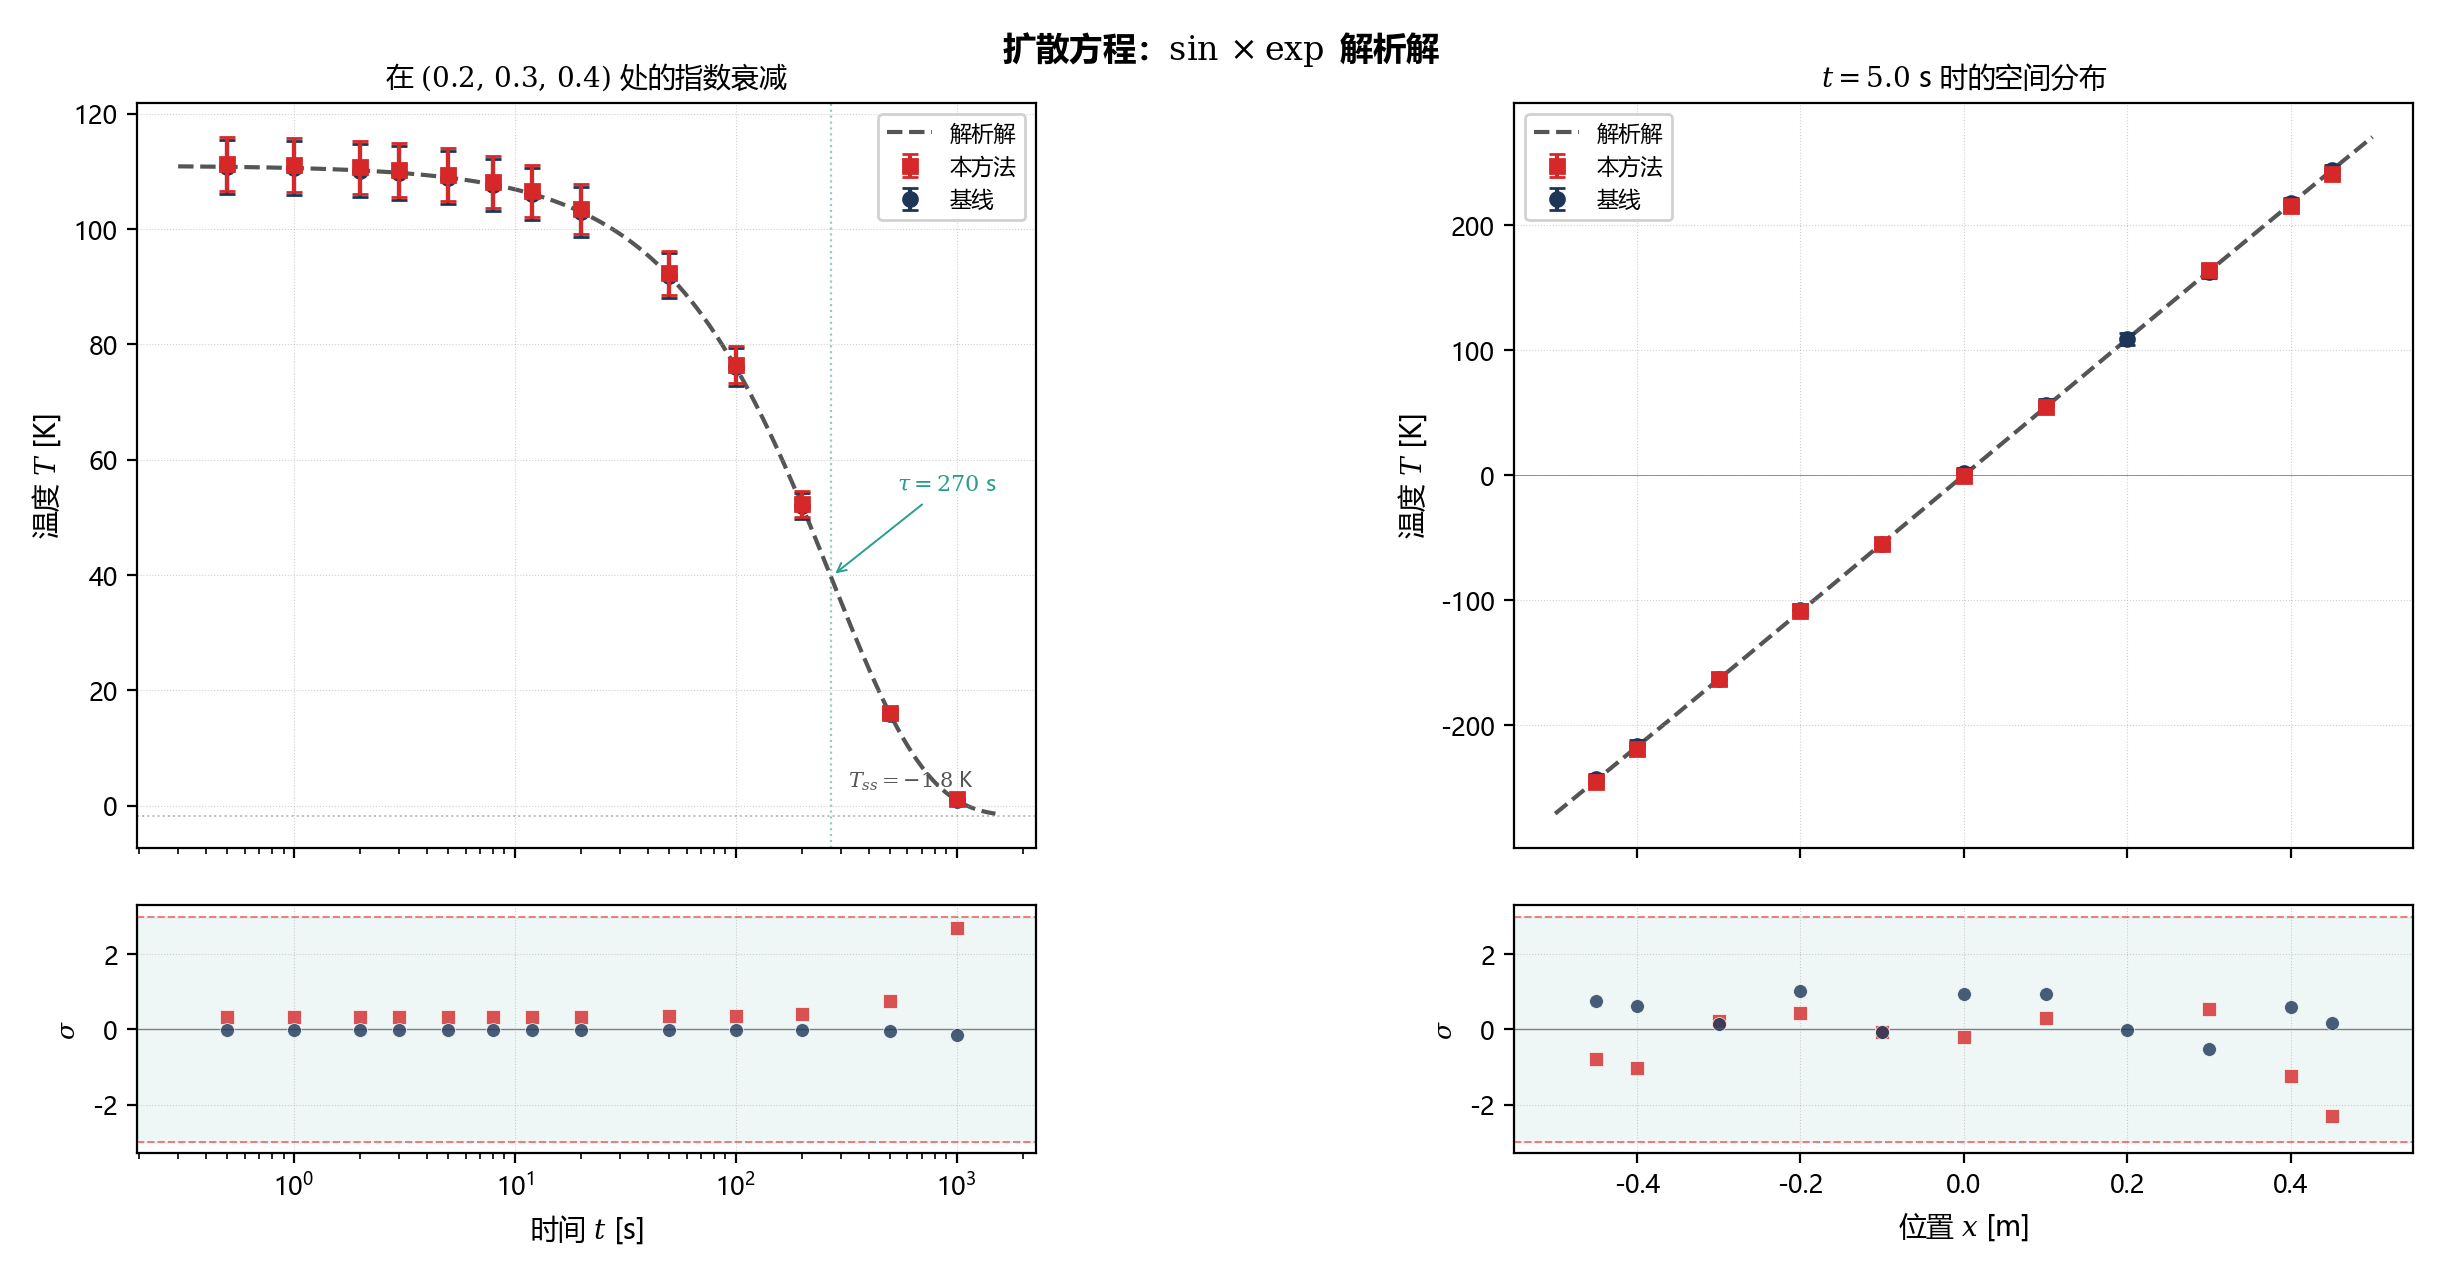
\includegraphics[width=0.9\textwidth]{Figures/Consistency/fig4_e3_sin_exp.png}
  \bicaption{扩散方程 $\sin \times \exp$ 精确解验证}{Diffusion equation $\sin \times \exp$ exact solution verification}
  \label{fig:consistency-sinexp}

  \small
  Wavefront 求解器（红色方块）与递归求解器（蓝色圆点）均精确复现时域指数衰减（左）与空间正弦分布（右）的解析解（灰色虚线），下方面板显示标准化偏差 $\sigma$ 均不超过 3。
\end{figure}

\paragraph{实验五：多域耦合瞬态——流体-固体-大气}

流体域、固体域与大气层组成的多介质耦合系统，从均匀初温 300~K 开始瞬态热响应。辐射边界条件驱动能量输入，参考值来自高精度数值求解。双探针设计揭示双时间尺度特征：流体探针 $(1.5, 1.5, 1.5)$ 接近辐射边界，约 3000~s 达稳态（$\sim$310~K）；固体探针 $(3.04, \cdot, \cdot)$ 热惯性大，超过 10000~s 仍在缓慢爬升（$\sim$305~K）。图~\ref{fig:consistency-e5} 展示了 0\textasciitilde10000~s 范围内两条趋近曲线，GPU（19/19）与 CPU（40/40）均精确跟踪参考曲线。该测试同时涵盖多域耦合、辐射边界条件、长时间瞬态和双时间尺度四个验证维度，是最接近工业真实场景的验证。

\begin{figure}[htbp]
  \centering
  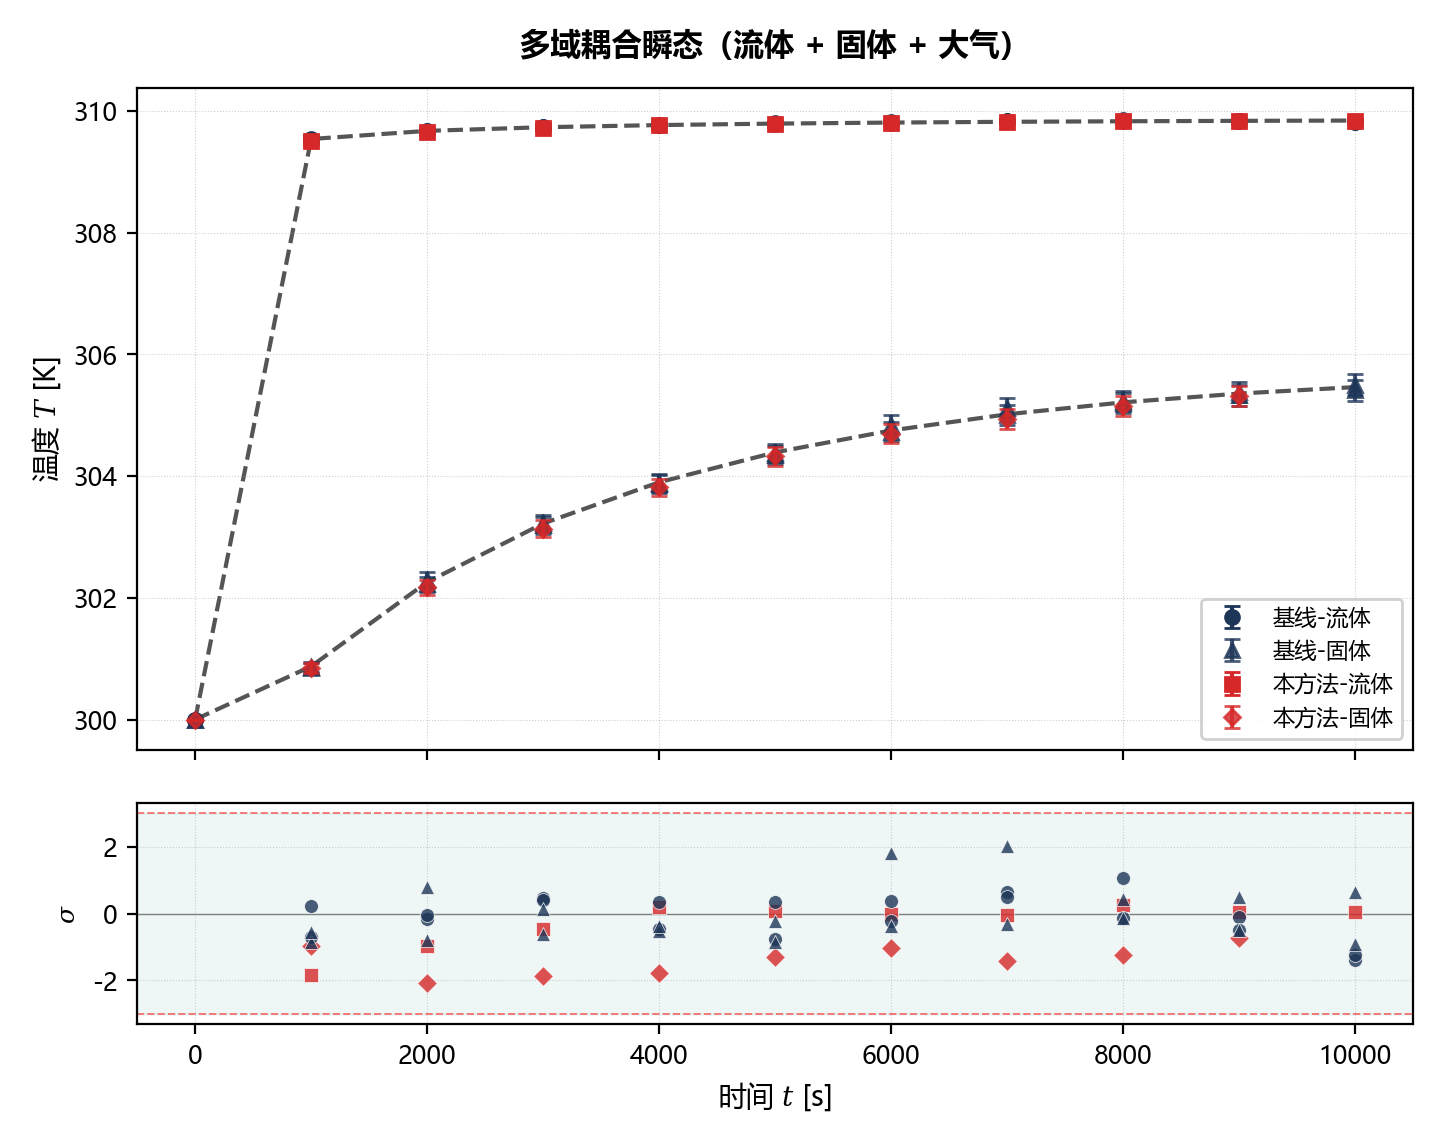
\includegraphics[width=0.85\textwidth]{Figures/Consistency/fig5_e5_multidomain.png}
  \bicaption{多域耦合瞬态验证}{Multi-domain transient verification}
  \label{fig:consistency-e5}

  \small
  流体探针（快响应，$\sim$3000~s 达稳态）与固体探针（慢响应，$>$10000~s）的温度演化均被两种架构精确复现，下方面板显示 $\sigma$ 均在 $\pm 3$ 以内。
\end{figure}

\paragraph{统计汇总}

表~\ref{tab:consistency-suite} 列出的 13 个场景按物理复杂度构成四级递进阶梯：第一级为单模态稳态（纯传导），覆盖体源、多材料异质性与介质嵌套，验证传导求解与材料处理的正确性；第二级为多模态稳态，引入辐射—传导耦合、Picard 多阶迭代与外部环境（太阳直射、天空漫射）边界，验证界面耦合与外部辐射条件的正确性；第三级引入时间维度，覆盖对流指数衰减、空间非均匀对流系数与扩散方程时空精确解，验证时间积分与瞬态边界的正确性；第四级为多域耦合瞬态全耦合场景，验证多介质域之间的完整耦合。前述 5 个详述实验已从各级中各选至少一个代表，优先采用具有封闭解析解的场景以提供最严格的基准对照；其余 8 个辅助测试在同级内覆盖正交参数变体，保证验证的系统性。全部 282 个有效数据点（GPU 134 + CPU 148）均通过 $3\sigma$ 检验。

GPU 和 CPU 的 $\sigma$ 均值分别为 0.816 和 0.739，最大标准化偏差分别为 2.708 和 2.676，均远低于 $3\sigma$ 阈值。图~\ref{fig:consistency-summary} 汇总全部 13 个测试的统计结果：左图 $\sigma$ 分布直方图显示两种架构分布形态高度一致，峰值集中于 $0$\textasciitilde$1\sigma$ 区间；右图 Parity 散点图中全量数据点紧密分布于 $E = T_{\mathrm{ref}}$ 对角线上，温度覆盖 $-244$~K 至 $2068$~K。

\begin{figure}[htbp]
  \centering
  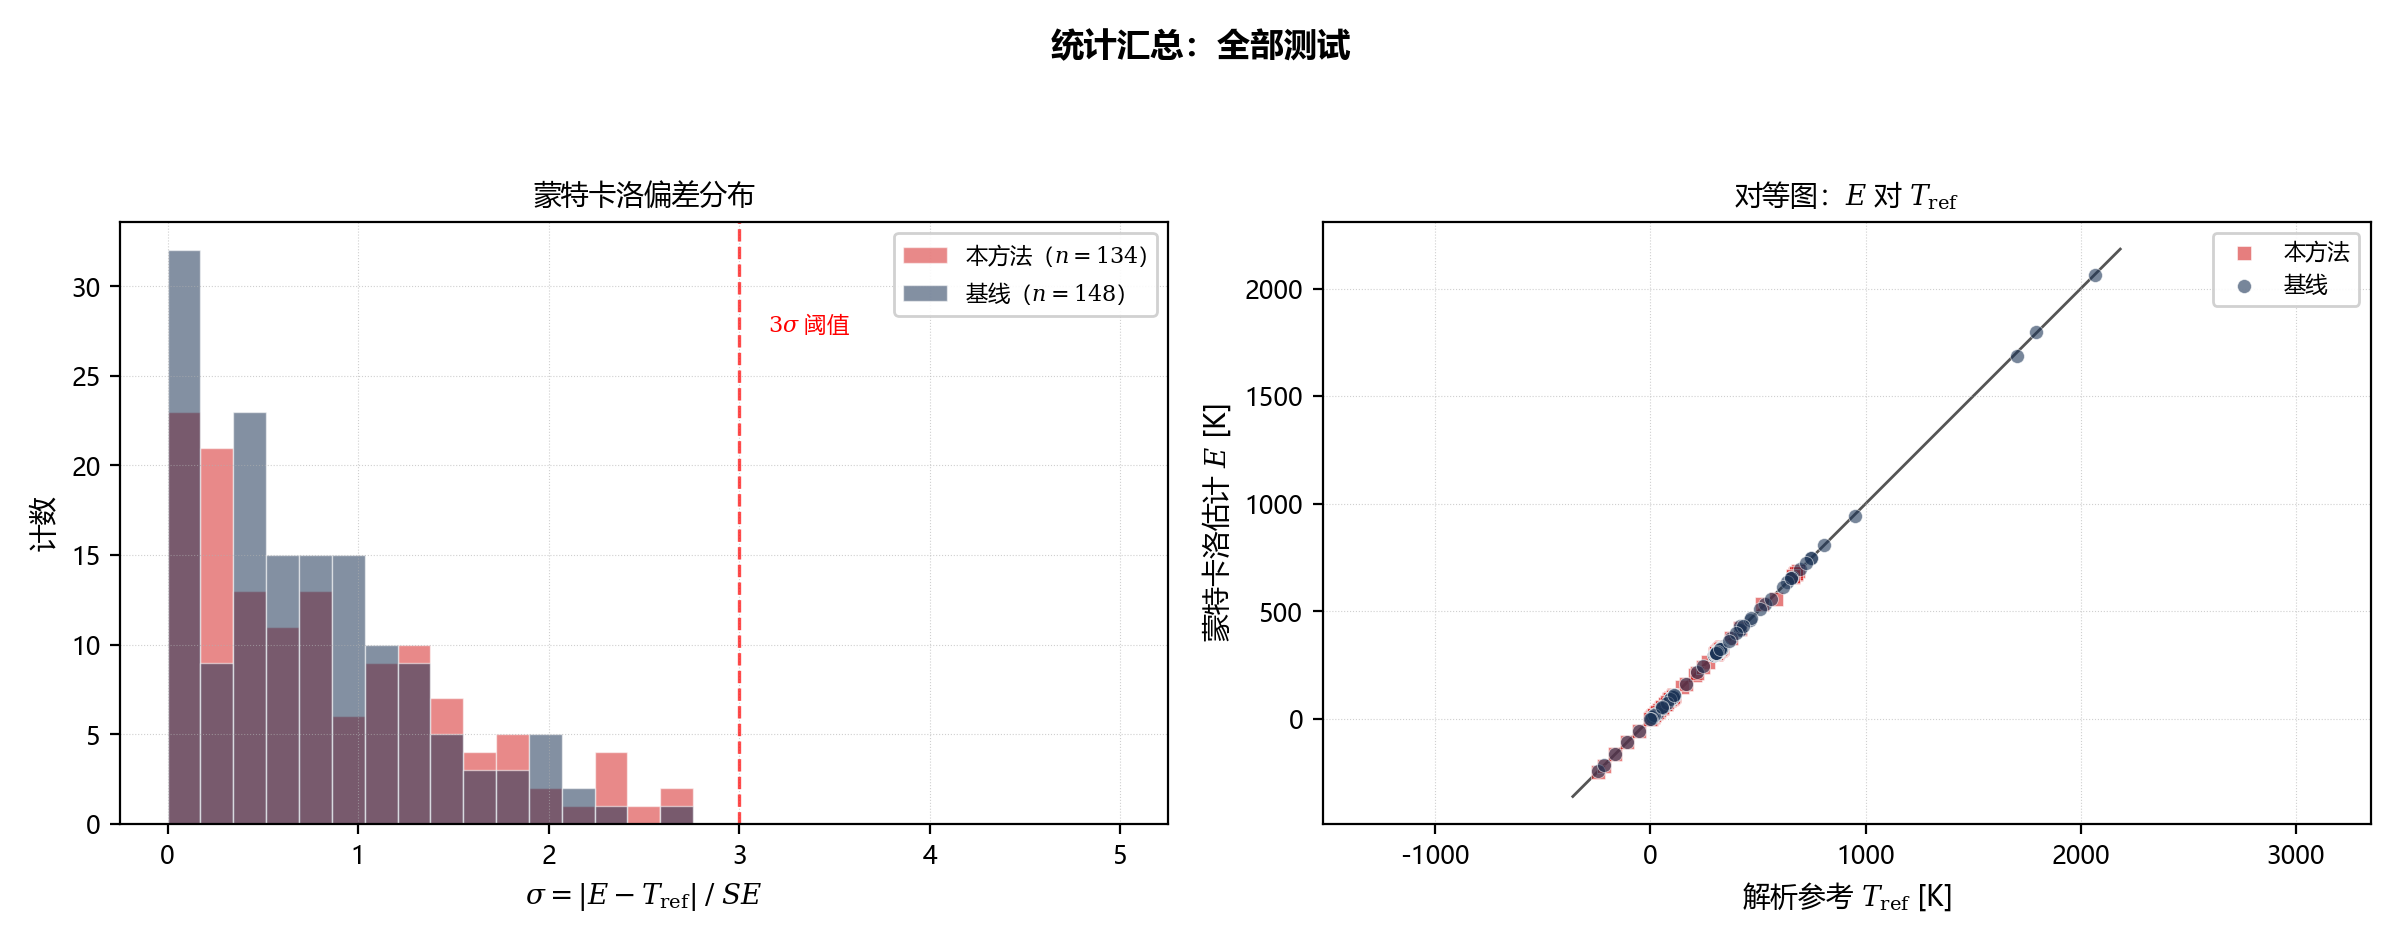
\includegraphics[width=0.9\textwidth]{Figures/Consistency/fig6_summary.png}
  \bicaption{全测试体系统计汇总}{Statistical summary of all tests}
  \label{fig:consistency-summary}

  \small
  (a) $\sigma$ 分布直方图——GPU 134 个与 CPU 148 个数据点均在 $3\sigma$ 阈值（红色虚线）以内；(b) 估计值 vs 参考值 Parity 散点图——全量数据点紧密分布于 $E = T_{\mathrm{ref}}$ 对角线。
\end{figure}

在共享探针位置的测试中，GPU 与 CPU 的标准误差（SE）比率为 $1.00 \pm 0.05$，确认两种架构的蒙特卡洛估计器方差结构等价——Wavefront 批处理与递归求解器逐路径两种调度策略不影响统计收敛行为。

\subsubsection{端到端统计等价性检验}

\paragraph{指标选择}

图像质量评估领域常用 PSNR（峰值信噪比）和 SSIM（结构相似性）作为衡量指标，它们以像素差的 $\ell_2$ 范数或局部结构相关性来量化两幅图像的``距离''。然而，这两类指标均不适用于蒙特卡洛求解器的等价性验证。原因在于：PSNR 和 SSIM 隐含一个确定性参考图（ground truth），将差异解读为确定性``失真''；而两个蒙特卡洛估计器对同一场景的输出本身就是随机变量——每个像素不仅有期望值，还有由采样量决定的标准误差。两幅蒙特卡洛图像之间的逐像素差异是两组随机变量之差，应使用假设检验框架判定其差异是否超出随机噪声的统计预期，而非用距离度量来衡量。此外，PSNR 依赖于信号动态范围，对于温度场（绝对温标，无界）缺乏自然的参考量程；SSIM 的局部窗口加权会平滑高频结构性偏差。

因此，本节采用逐像素双样本 $Z$ 检验：对 Wavefront 求解器和递归求解器输出的每个像素独立构造检验统计量，利用蒙特卡洛估计器自身提供的标准误差进行归一化，直接判定差异是否可由随机抽样噪声解释。

\paragraph{检验方法}

在 porous 场景（$512 \times 512$，128 SPP）上，对 Wavefront 求解器和递归求解器的逐像素估计量进行双样本 $Z$ 检验：

\begin{equation}
  \label{eq:z-test}
  Z_{x,y} = \frac{|E_{\mathrm{gpu}} - E_{\mathrm{cpu}}|}{\sqrt{\mathrm{SE}_{\mathrm{gpu}}^2 + \mathrm{SE}_{\mathrm{cpu}}^2}}
\end{equation}

\noindent 其中 $E$ 为像素温度估计值，$\mathrm{SE}$ 为蒙特卡洛标准误差。若两种架构的估计器无偏且等价，$Z_{x,y}$ 应服从标准半正态分布（$|Z|$ 分布），在显著性水平 $\alpha = 0.05$ 下期望仅约 5\% 的像素因随机噪声被``误拒''。共 262{,}144 个像素中有 153{,}976 个有效像素（排除背景和零方差像素）。

\paragraph{多重比较校正}

逐像素检验涉及 $N = 153{,}976$ 次独立假设检验，属于典型的大规模多重比较问题。若不加校正，在 $\alpha = 0.05$ 下纯随机噪声即可产生约 $0.05 \times 153{,}976 \approx 7{,}699$ 个``假阳性''像素，使得单像素显著性失去判断能力。为此采用两种互补的多重比较校正方法：

\textbf{Bonferroni 校正}是最保守的全族错误率（FWER）控制方法：将每个像素的显著性阈值收紧为 $\alpha/N$，即 $\alpha_{\mathrm{Bonf}} = 0.05/153{,}976 \approx 3.25 \times 10^{-7}$，对应的 $Z$ 阈值约为 5.05。它控制的是``至少一个假阳性''的概率不超过 $\alpha$——只要有任一像素的 $Z$ 值超过 5.05，就有充分理由怀疑系统性偏差存在。Bonferroni 校正虽然以牺牲统计功效为代价换取极强的保守性，但这恰恰符合本文的验证需求：我们不关心``多少像素有差异''，而关心``是否存在任何真实差异''。

\textbf{Benjamini-Hochberg (BH) 假发现率（FDR）校正}控制的是在拒绝集合中假阳性所占比例的期望值不超过 $q$（本文取 $q = 0.05$）。其步骤为：将 $N$ 个 $p$ 值从小到大排序为 $p_{(1)} \leq \cdots \leq p_{(N)}$，找到满足 $p_{(k)} \leq k \cdot q / N$ 的最大 $k$，拒绝前 $k$ 个假设。BH-FDR 比 Bonferroni 宽松，统计功效更高，若它也报告零显著像素，则进一步排除了 Bonferroni 过于保守而遗漏弱信号的可能性。两种校正方法从严-宽两个极端形成包夹：Bonferroni 保证无假阳性，BH-FDR 保证不遗漏成片的弱偏差。

\paragraph{检验结果}

表~\ref{tab:pixel-consistency} 汇总了检验结果。

\begin{table}[htbp]
  \centering
  \bicaption{porous 场景逐像素统计等价性检验结果}{Per-pixel statistical equivalence test results on the porous scene}
  \label{tab:pixel-consistency}
  \small
  \begin{tabular}{lcc}
    \toprule
    指标 & 结果 & 纯 MC 噪声期望值 \\
    \midrule
    有效像素数                          & 153{,}976               & — \\
    Mean $Z$                            & 0.8057                  & $\sim$0.7979（半正态均值）\\
    原始拒绝率 ($\alpha = 0.05$)        & 5.10\%                  & $\sim$5\% \\
    Bonferroni 校正后显著像素           & \textbf{0}              & $\sim$0 \\
    Benjamini-Hochberg FDR 校正后显著像素 & \textbf{0}            & $\leq$5\% \\
    \bottomrule
  \end{tabular}
\end{table}

Mean $Z = 0.8057$ 与理论半正态均值 $\sqrt{2/\pi} \approx 0.7979$ 的偏差仅为 1.0\%，表明 $Z$ 值分布与零假设预测精确吻合。原始拒绝率 5.10\% 与 $\alpha = 0.05$ 的预期一致，无超额拒绝。经 Bonferroni 校正（$Z$ 阈值 $\approx 5.05$）后零显著像素，说明不存在任何单像素级别的系统性偏差；经 BH-FDR 校正后同样零显著像素，排除了成片弱偏差被 Bonferroni 遗漏的可能。判定结果为PASS (strong)：两架构的逐像素差异完全落入蒙特卡洛随机噪声范围。

图~\ref{fig:pixel-consistency} 展示 porous 场景的逐像素诊断结果：$Z$ 值直方图（左）与半正态 Q-Q 图（右）。直方图中观测 $Z$ 分布（蓝色柱）与理论半正态分布（黑色虚线）高度吻合，$z = 1.96$（$\alpha = 0.05$ 阈值）和 Bonferroni 校正阈值以虚线标注，无任何数据点超过后者；Q-Q 图中绝大多数数据点沿对角线紧密排列，尾部无系统性偏离，确认无结构性偏差。

\begin{figure}[htbp]
  \centering
  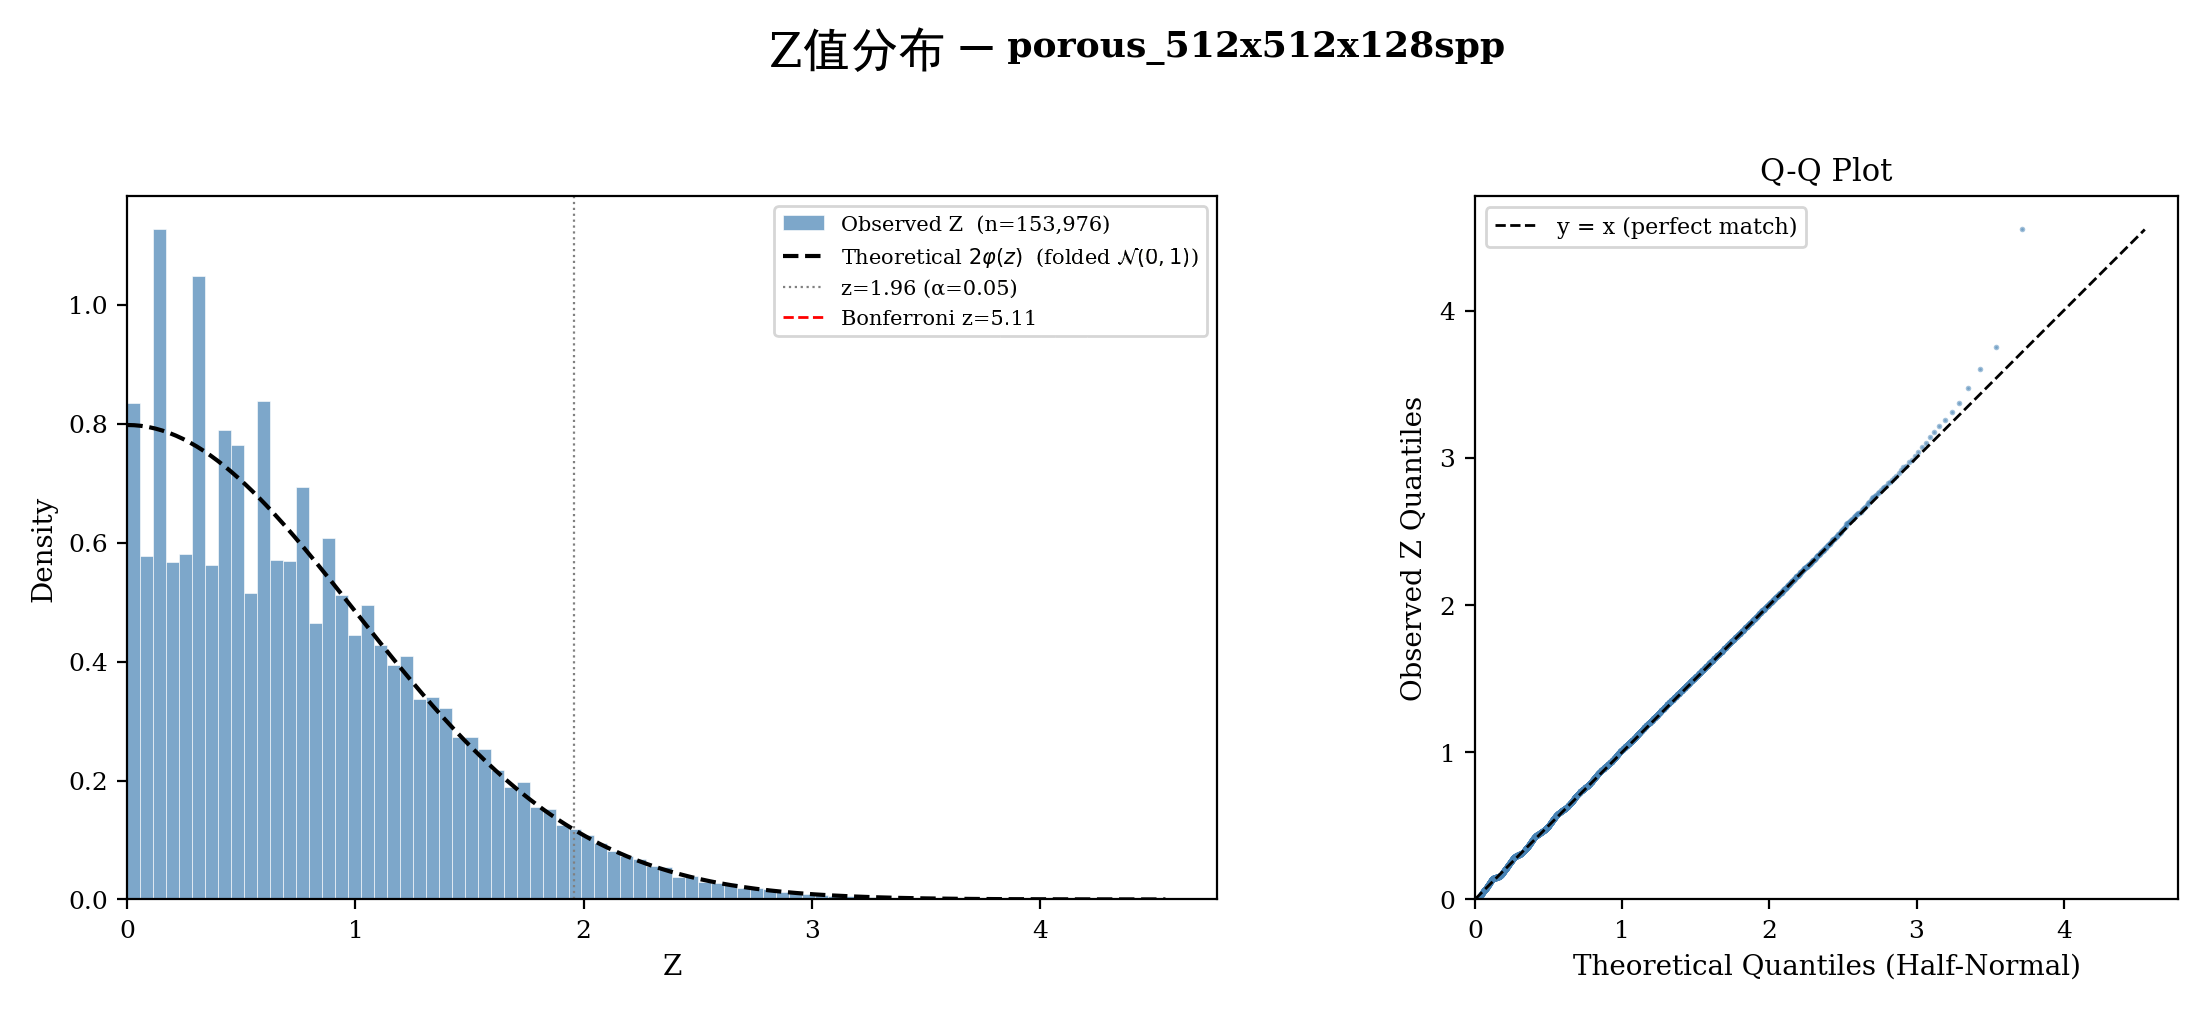
\includegraphics[width=0.85\textwidth]{Figures/Consistency/porous_512x512x128spp_z_diagnostic.png}
  \bicaption{porous 场景逐像素 $Z$ 值诊断（$512 \times 512$，128 SPP）}{Per-pixel $Z$ diagnostic for the porous scene ($512 \times 512$, 128 SPP)}
  \label{fig:pixel-consistency}

  \small
  左图：$Z$ 分布直方图，与半正态理论分布高度吻合，$z = 1.96$（$\alpha = 0.05$）和 Bonferroni 校正阈值以虚线标注；右图：半正态 Q-Q 图，数据点沿对角线紧密排列。
\end{figure}

图~\ref{fig:difference-map} 以空间视图呈现上述统计检验的直观对应：上排分别为 Wavefront 求解器和递归求解器的渲染温度场，视觉上难以分辨差异；下排左图为逐像素绝对温差 $|E_{\mathrm{gpu}} - E_{\mathrm{cpu}}|$，下排右图为逐像素 $Z$ 值空间分布。温差图呈现均匀的低幅噪声纹理，$Z$ 值图中无任何空间聚集的高值区域——这排除了局部几何死角或特定物理模块引入结构性偏差的可能。若 Wavefront 架构在某一物理模块（如 BND 界面耦合或 ENC 包壳查询）存在实现缺陷，对应几何区域的 $Z$ 值将系统性偏高并形成空间聚集，而图中完全不存在这种模式。

\begin{figure}[htbp]
  \centering
  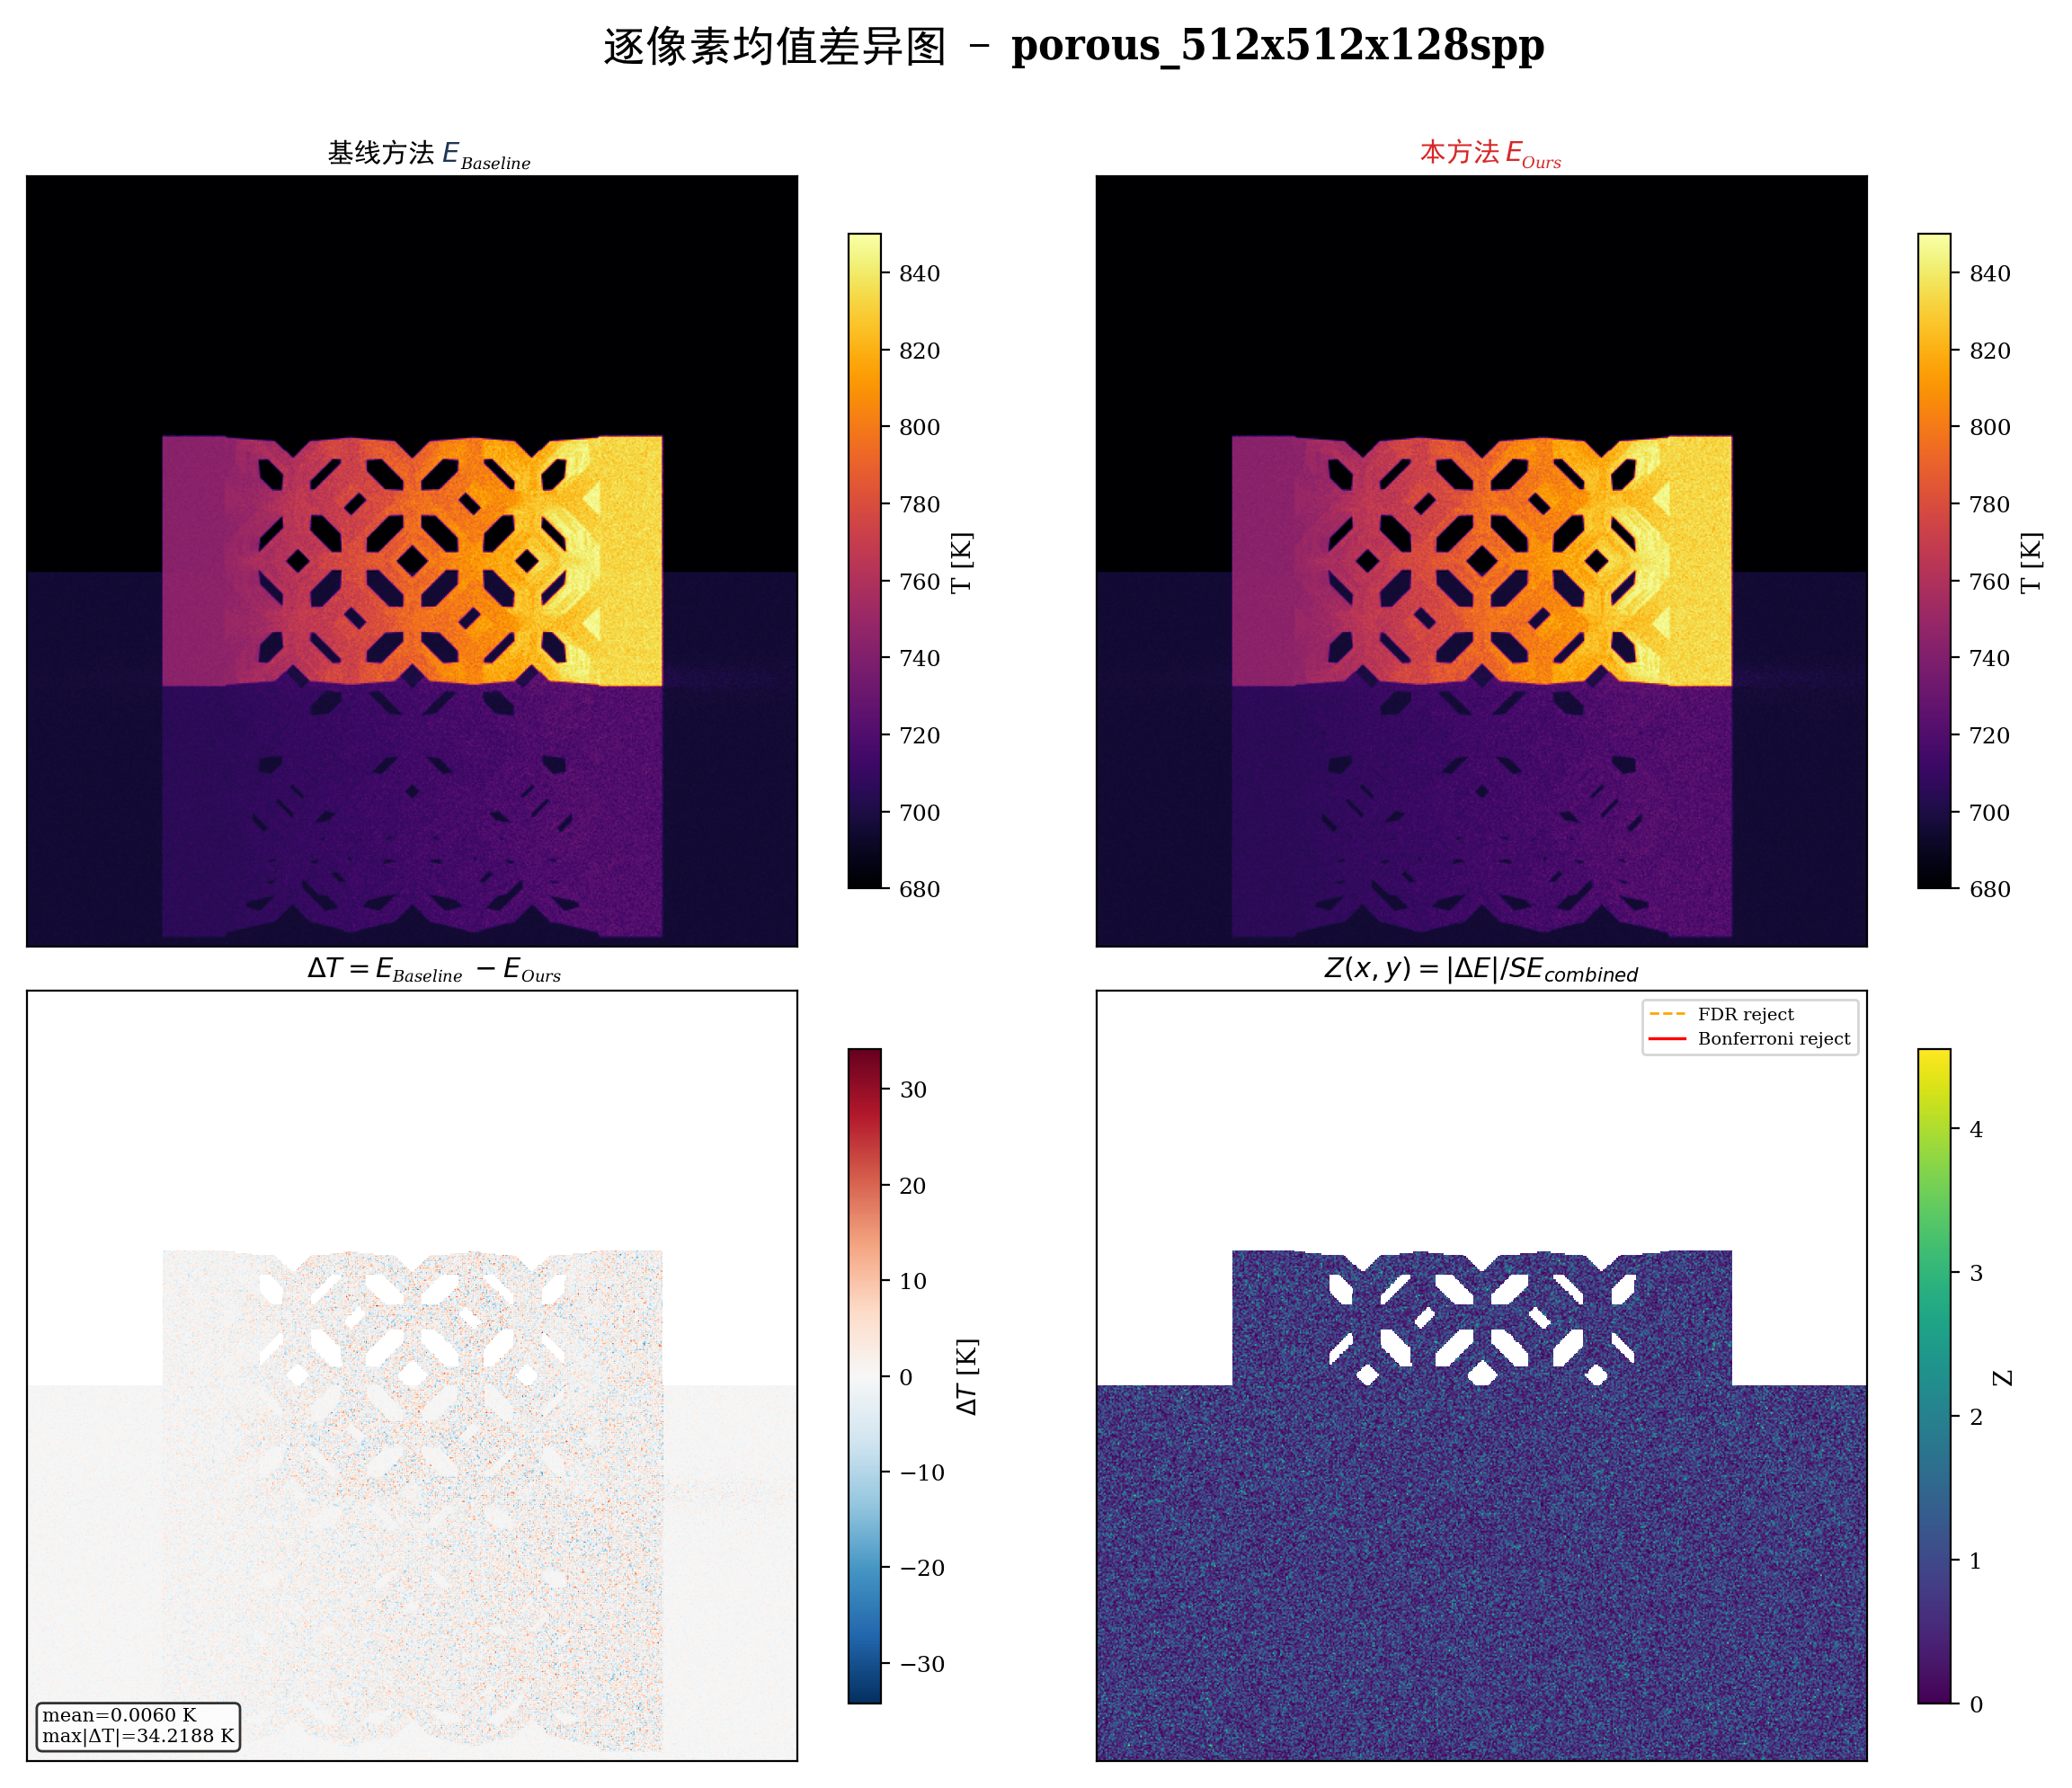
\includegraphics[width=0.9\textwidth]{Figures/Consistency/porous_512x512x128spp_difference_map.png}
  \bicaption{porous 场景逐像素对比（$512 \times 512$，128 SPP）}{Per-pixel comparison of the porous scene ($512 \times 512$, 128 SPP)}
  \label{fig:difference-map}

  \small
  上排：Wavefront 求解器（左）与递归求解器（右）渲染温度场，视觉不可分辨；下排：逐像素绝对温差（左）与 $Z$ 值空间分布（右），差异呈均匀随机噪声，无空间聚集结构。
\end{figure}

综合两个维度的验证结果：物理过程验证证明 Wavefront 实现无系统性物理偏差（13 场景，282 数据点，100\% 通过 $3\sigma$）；端到端统计检验证明两架构在真实耦合场景中的逐像素结果统计等价（153{,}976 有效像素，多重比较校正后零显著差异）。Wavefront 架构改造不引入物理偏差。

\subsection{性能分析}

\subsubsection{端到端性能对比}

表~\ref{tab:performance-comparison} 给出 porous 场景（$320 \times 320$，32 SPP）在不同 CPU 线程数和路径池容量下的端到端墙钟时间和加速比。

\begin{table}[htbp]
  \centering
  \bicaption{porous 场景端到端性能对比}{End-to-end performance comparison on the porous scene}
  \label{tab:performance-comparison}
  \small
  \begin{tabular}{llccc}
    \toprule
    方案 & Pool Size & 线程数 & 墙钟时间 (s) & 加速比 $S$ \\
    \midrule
    Baseline (递归求解器+Embree)  & —      & 32 & 106 & 1.00$\times$ \\
    Baseline (递归求解器+Embree)  & —      & 16 & 155 & 1.00$\times$ \\
    Baseline (递归求解器+Embree)  & —      & 8  & 215 & 1.00$\times$ \\
    \midrule
    Ours (WF+OptiX)        & 8{,}192  & 32 & 104 & 1.02$\times$ \\
    Ours (WF+OptiX)        & 8{,}192  & 16 & 116 & 1.34$\times$ \\
    Ours (WF+OptiX)        & 8{,}192  & 8  & 157 & 1.37$\times$ \\
    \midrule
    Ours (WF+OptiX)        & 16{,}384 & 32 & 234 & 0.45$\times$ \\
    \midrule
    WF+Embree（消融）       & 8{,}192  & 32 & 426 & 0.25$\times$ \\
    \bottomrule
  \end{tabular}
\end{table}

数据呈现三个层次的现象：

（1）在 8\textasciitilde 16 线程的典型工作站配置下，Ours 取得显著加速：8 线程为 $1.37\times$，16 线程为 $1.34\times$。Baseline 的并行度直接受限于 CPU 核心数，其性能随线程数近似线性退化（$155/106 \approx 1.46\times$、$215/106 \approx 2.03\times$）；Ours 的 GPU 查询吞吐不受 CPU 线程数约束，GPU 卸载收益在中等线程配置下最为突出。

（2）当 CPU 线程数达到 32（i9-13900K 全部核心）时，加速比为 $1.02\times$，两种架构达到性能均势（parity）。Baseline 已充分利用全部核心与 Embree 高度优化的 SIMD 光追，CPU 侧状态管理开销抵消了 GPU 查询吞吐增益。

（3）路径池容量从 8{,}192 增至 16{,}384 后，32 线程下墙钟时间从 104~s 跃升至 234~s（$2.25\times$ 退化），退化幅度远超池容量翻倍本身。这是工作集突破缓存容量阈值后的典型 Cache Cliff 行为，直接证明 CPU 缓存压力是主导性能约束。

\subsubsection{$T_A / T_B$ 时间分解}

为定量分析 Wavefront 管线的时间构成，本节将主循环每轮迭代耗时分解为 CPU 状态推进耗时 $T_A$（merged\_pass $+$ compact $+$ housekeeping）和 GPU 设备侧查询耗时 $T_B^{\text{dev}}$（kernel 执行 $+$ D2H 传输 $+$ launch 开销），以及 CPU 侧查询后处理耗时 $T_B^{\text{host}}$（trace\_post）。在双池 Ping-Pong 模式下，$T_A$ 与 $T_B^{\text{dev}}$ 可通过交替调度重叠执行。

表~\ref{tab:time-breakdown} 报告了 porous 场景（$320 \times 320$，32 SPP，32 线程）在不同路径池容量下的时间分解数据。每组配置运行 3 次取中位数。

\begin{table}[htbp]
  \centering
  \bicaption{Wavefront 管线 $T_A / T_B$ 时间分解（porous 场景，32 线程，双池模式）}{$T_A / T_B$ time decomposition of the Wavefront pipeline (porous scene, 32 threads, dual-pool mode)}
  \label{tab:time-breakdown}
  \small
  \begin{tabular}{rrrrrr}
    \toprule
    池容量 & $T_A$ (s) & $T_B^{\text{dev}}$ (s) & $T_B^{\text{host}}$ (s) & $T_A / T_B^{\text{dev}}$ & Wall (s) \\
    \midrule
    1{,}024  & 229.7 & 44.8 & 101.6 & 5.1$\times$ & 392.1 \\
    2{,}048  & 140.6 & 22.8 & 57.1  & 6.2$\times$ & 227.4 \\
    4{,}096  & 93.7  & 15.2 & 22.3  & 6.1$\times$ & 134.4 \\
    \textbf{8{,}192}  & \textbf{77.0}  & \textbf{11.8} & \textbf{17.5}  & \textbf{6.5$\times$} & \textbf{108.6} \\
    16{,}384 & 131.7 & 8.6  & 19.3  & 15.3$\times$ & 161.6 \\
    32{,}768 & 190.2 & 10.4 & 28.1  & 18.4$\times$ & 230.8 \\
    \midrule
    8{,}192（单池） & 64.2  & 63.8 & 13.6  & 1.0$\times$ & 169.2 \\
    \bottomrule
  \end{tabular}
\end{table}

数据显示，在所有双池配置下均有 $T_A \gg T_B^{\text{dev}}$（5.1\textasciitilde 18.4 倍），GPU 查询管线的设备侧耗时始终被 CPU 侧完全覆盖——GPU 并非性能瓶颈。$T_A$ 的主要成分为 merged\_pass（占 $T_A$ 的 87\%\textasciitilde 92\%），即逐路径遍历路径池执行状态机转移和请求/结果读写的 Cache 密集型操作。这直接证明了 CPU 侧状态推进的内存访问模式是瓶颈所在，也解释了第四章报告的 333 倍 RT 查询吞吐优势为何未能转化为等比例的端到端加速：GPU 查询管线的设备侧耗时（$T_B^{\text{dev}} = 11.8$~s，池容量 8{,}192）仅占墙钟时间的 10.9\%，即使将 $T_B^{\text{dev}}$ 优化至零，端到端加速上界也仅为 $108.6 / (108.6 - 11.8) = 1.12\times$。

\subsubsection{路径池容量扫描}

表~\ref{tab:pool-scan} 给出路径池容量从 1{,}024 到 32{,}768（按 2 的幂次）的连续扫描结果，完整展现 Cache Cliff 效应的临界点。

\begin{table}[htbp]
  \centering
  \bicaption{路径池容量连续扫描（porous 场景，32 线程，双池模式）}{Pool size sweep (porous scene, 32 threads, dual-pool mode)}
  \label{tab:pool-scan}
  \small
  \begin{tabular}{rrrrr}
    \toprule
    池容量 & 墙钟时间 (s) & 迭代轮数 & Refill 阶段 (s) & Drain 阶段 (s) \\
    \midrule
    1{,}024  & 392 & 3{,}258{,}343 & 384 & 8 \\
    2{,}048  & 227 & 1{,}668{,}672 & 217 & 10 \\
    4{,}096  & 134 & 875{,}364    & 122 & 12 \\
    \textbf{8{,}192}  & \textbf{104} & \textbf{482{,}079} & \textbf{89} & \textbf{15} \\
    16{,}384 & 161 & 290{,}795    & 139 & 22 \\
    32{,}768 & 231 & 197{,}059    & 188 & 43 \\
    \bottomrule
  \end{tabular}
\end{table}

池容量 8{,}192 为最优工作点（104~s），此时工作集（25\textasciitilde 32~MB）接近 L2 Cache 容量上限。向左（池更小）：迭代轮数激增（每轮可积累的查询量少），每轮 Refill 阶段的循环调度开销（compact $+$ housekeeping）成为瓶颈。向右（池更大）：工作集突破 L2/L3 缓存容量阈值，merged\_pass 遍历产生大量 LLC Miss，尽管迭代轮数减少但单轮耗时剧增。

\subsubsection{单池 vs. 双池消融实验}

表~\ref{tab:single-dual} 给出池容量 8{,}192 下单池与双池（Ping-Pong）模式的对比。

\begin{table}[htbp]
  \centering
  \bicaption{单池 vs. 双池消融实验（porous 场景，32 线程，池容量 8{,}192）}{Single-pool vs.\ dual-pool ablation (porous scene, 32 threads, pool size 8{,}192)}
  \label{tab:single-dual}
  \small
  \begin{tabular}{lrrrr}
    \toprule
    模式 & $T_A$ (s) & $T_B^{\text{dev}}$ (s) & $T_A / T_B^{\text{dev}}$ & Wall (s) \\
    \midrule
    单池 & 64.2  & 63.8 & 1.0$\times$ & 169.2 \\
    双池 & 77.0  & 11.8 & 6.5$\times$ & 108.6 \\
    \bottomrule
  \end{tabular}
\end{table}

单池模式下 $T_A \approx T_B^{\text{dev}}$（1.0$\times$），CPU 与 GPU 串行执行，无重叠——每轮须等 GPU 完成后才能继续推进路径。双池模式下引入第二个 View 后，GPU 计算被完全隐藏在 CPU 推进期间（$T_A / T_B^{\text{dev}} = 6.5\times$），墙钟时间从 169.2~s 降至 108.6~s（$\mathbf{36\%}$ 改善）。双池的 $T_A$ 较单池高 20\%（77.0 vs 64.2~s），源于双池切换和同步点引入的额外开销，但该开销被延迟隐藏收益充分覆盖。

\subsubsection{查询后端消融：WF + Embree vs.\ WF + OptiX}
\label{sec:wf-embree-ablation}

为隔离 Wavefront 架构改造引入的 Cache 代价与 GPU 后端的吞吐收益，本节将 Wavefront 求解器的查询后端从 OptiX 替换为 Embree，构成"递归 + Embree $\to$ WF + Embree $\to$ WF + OptiX"三点证据链。Wavefront 求解器的查询后端接口（submit / sync / retrieve）在设计上是设备无关的，Embree 后端与 OptiX 后端通过该接口完全兼容。由于 Embree 与 Wavefront 状态机均在 CPU 上执行，双池 Ping-Pong 异步重叠无意义，因此 WF + Embree 仅使用单池模式。为验证结论对线程配置的鲁棒性，实验同时在 32 线程（满配）与 16 线程（典型工作站）下执行。

表~\ref{tab:wf-embree-ablation} 列出各配置的端到端墙钟时间，并附 $T_A$（CPU 状态推进耗时）与 $T_B^{\text{dev}}$（查询引擎设备侧执行耗时）以揭示管线解耦特性。$T_A$ 定义同表~\ref{tab:time-breakdown}；$T_B^{\text{dev}}$ 对 WF + Embree 为多线程 CPU 查询执行耗时，对 WF + OptiX 为 GPU 管线耗时（kernel $+$ D2H $+$ launch）。

\begin{table}[htbp]
  \centering
  \bicaption{查询后端消融实验（porous 场景，$320 \times 320$，32 SPP，池容量 8{,}192）}{Query backend ablation (porous scene, $320 \times 320$, 32 SPP, pool size 8{,}192)}
  \label{tab:wf-embree-ablation}
  \small
  \begin{tabular}{llrrrrr}
    \toprule
    架构 & 查询后端 & 线程 & $T_A$ (s) & $T_B^{\text{dev}}$ (s) & Wall (s) & vs Baseline \\
    \midrule
    递归 & Embree（逐条）     & 32 & —    & —     & 106 & $1.00\times$ \\
    WF 单池 & Embree（批量） & 32 & 63.4 & 326.4 & 426 & $0.25\times$ \\
    WF 单池 & OptiX（批量）  & 32 & 64.2 & 63.8  & 169 & $0.63\times$ \\
    WF 双池 & OptiX（批量）  & 32 & 77.0 & 11.8  & 104 & $1.02\times$ \\
    \midrule
    递归 & Embree（逐条）     & 16 & —    & —     & 155 & $1.00\times$ \\
    WF 单池 & Embree（批量） & 16 & 73.4 & 535.1 & 642 & $0.24\times$ \\
    WF 单池 & OptiX（批量）  & 16 & 72.6 & 65.7  & 179 & $0.87\times$ \\
    WF 双池 & OptiX（批量）  & 16 & —    & —     & 116 & $1.34\times$ \\
    \bottomrule
  \end{tabular}
\end{table}

表中 $T_A$ 列呈现本节最核心的发现——CPU 状态推进与查询后端的彻底解耦。在控制线程数与池模式的条件下，Embree 后端与 OptiX 后端的 $T_A$ 高度一致：32 线程下 63.4~s vs 64.2~s（偏差 $\pm 1.3\%$），16 线程下 73.4~s vs 72.6~s（偏差 $\pm 1.1\%$）。$T_A$ 的主要成分 merged\_pass（占 87\%\textasciitilde 92\%）是逐路径遍历路径池执行状态机转移的 Cache 密集型操作，其耗时取决于路径池容量与 \texttt{path\_state} 访存模式，与查询引擎无关——$T_A$ 不随后端变化是 Wavefront 解耦架构的直接定量证据。

$T_B^{\text{dev}}$ 列揭示查询引擎层面的性能差距及其与 CPU 线程数的关系。Embree 批量计算耗时随可用线程减半而显著增长（326.4 $\to$ 535.1~s，$+64\%$），GPU 管线几乎不受影响（63.8 $\to$ 65.7~s，$+3\%$）。由此，Embree 与 OptiX 单池的查询阶段倍率从 32 线程的 $5.1\times$（$326.4/63.8$）扩大至 16 线程的 $8.1\times$（$535.1/65.7$）。在端到端层面，Ours（双池）在 16 线程下达到 $1.34\times$ 加速——GPU 卸载的边际收益随 CPU 并行度降低而放大。递归 $\to$ WF + Embree 的退化倍率在两种线程配置下高度一致（$4.0\times$ / $4.1\times$），确认 Wavefront 架构的 Cache 代价是结构性的、与线程数无关的固有特征。

上述数据同时印证了批量化对不同后端的非对称影响。递归求解器中 Embree 以逐条模式（\texttt{rtcIntersect1}）执行，局部状态驻留在线程栈中，Cache 亲和性高；Wavefront 批量模式下查询通过数组遍历提交，Cache 局部性下降导致 Embree 有效吞吐退化。GPU 后端不受此影响——批量化正是 GPU 硬件的优势执行模式，RT Core 天然适配大批量并行查询。双池 Ping-Pong 的收益在两种线程配置下同样稳定（32 线程 $1.6\times$、16 线程 $1.5\times$）。整条证据链完整覆盖了从暴露 Cache 代价到恢复并超越 Baseline 的性能路径：GPU 后端与双池异步调度不仅是弥补 Wavefront Cache 代价的充分条件，在典型工作站配置下更实现了净加速。

\subsubsection{端到端加速比随场景规模的趋势分析}
\label{sec:scene-scale-analysis}

当前端到端性能评估仅使用了 porous 场景（13{,}010 面片），这一局限的根本原因在于耦合热输运仿真的测试场景需要完整的物理配置文件（材质参数、边界条件、腔体归属、对流系数等），这些配置无法自动生成，均须手工标注。本文 13 个一致性验证场景已覆盖全部物理模块，但构造更大规模的工程场景超出了论文时间范围。

尽管如此，端到端加速比中场景复杂度仅影响 $T_B$（GPU 查询阶段），不影响 $T_A$（CPU 状态推进阶段）。Wavefront 主循环的 CPU 侧工作逐路径遍历路径池数组，执行状态机转移和请求/结果的读写，其耗时由路径池容量和 \texttt{path\_state} 结构体的 Cache 访问模式决定，与场景的三角面片数量无关。当场景规模增大时，BVH 深度增加导致 $T_B$ 增长，但 $T_A$ 保持不变。端到端加速比 $S_{\text{e2e}}$ 可表示为：

\begin{equation}
  \label{eq:speedup-trend}
  S_{\text{e2e}} = \frac{T_A^{\text{baseline}} + T_B^{\text{baseline}}}{T_A^{\text{ours}} + \max(T_A^{\text{ours}}, T_B^{\text{ours}})}
\end{equation}

当场景规模增大使 $T_B^{\text{baseline}}$ 显著增长时（CPU Embree 的 BVH 遍历受 SIMD 宽度限制，其性能随 BVH 深度退化显著快于 RT Core 硬件加速），分子增长快于分母，$S_{\text{e2e}}$ 单调增长。这表明 porous 场景（13{,}010 面片）实际上是对本方法最不利的测试条件——GPU 优势尚未充分发挥，而 CPU 侧 Cache 代价已完全暴露。更大规模场景下 GPU 优势预计更为显著。

\subsubsection{Cache 压力瓶颈分析}

上述现象的根本原因在于递归求解器与 Wavefront 求解器两种架构在内存访问模式上的本质差异。递归求解器同一时刻仅维护一条路径的状态，所有局部变量驻留在函数调用栈中，自然命中 L1/L2 Cache，内存访问效率极高。Wavefront 架构中路径池的 8{,}192 条 \texttt{path\_state} 结构体构成的工作集（单条约 3\textasciitilde 4~KB，总计约 25\textasciitilde 32~MB）接近 i9-13900K 的 L2 Cache 总量（约 32~MB），每轮 advance/cascade/distribute 遍历路径池时产生大量末级缓存缺失（LLC Miss）。当池容量翻倍至 16{,}384 条时，工作集超过 50~MB，远超 L2 容量并开始显著溢出 L3 Cache（36~MB），导致性能剧烈退化。

Cache 压力是 CPU 侧实例化的固有约束，而非 Wavefront 架构本身的缺陷。Wavefront 解耦是批量化的前提，持久化路径状态是解耦的必要条件，而路径池的规模直接决定了每批次可积累的几何查询量。在 CPU 侧，工作集受限于末级缓存容量（36~MB）；在全 GPU 实现中，路径状态常驻显存（RTX 4090: 24~GB），工作集约束放宽近三个数量级，上述瓶颈将从根本上消除。因此，Cache 压力是 CPU 侧实例化的实现约束，而非架构层面的设计缺陷——以路径状态的持久化开销换取几何查询的批量化能力，是 Wavefront 架构的核心设计选择。

\subsubsection{架构意义}

端到端实验结果在验证架构正确性之外，同时揭示了当前 CPU 侧实例化方案的性能特征与优化空间：

（1）\emph{架构正确性}。3.4.2 的一致性验证已充分证明 Wavefront 改造不引入物理偏差。端到端性能数据确认该架构可在真实场景中稳定运行并产生正确结果。

（2）\emph{典型配置下的实用加速}。在 8\textasciitilde 16 线程的典型工作站配置下，Ours 实现 $1.3$\textasciitilde$1.4\times$ 加速，GPU 查询吞吐有效补偿了 CPU 并行度不足。

（3）\emph{瓶颈精准定位与解耦验证}。端到端数据结合 Pool Size 对比实验，定量证明当前性能瓶颈位于 CPU 侧状态管理的 Cache Miss，而非 GPU 查询吞吐或 PCIe 传输延迟。查询后端消融实验（表~\ref{tab:wf-embree-ablation}）的 $T_A$ 列从四组受控对比（2 后端 $\times$ 2 线程配置）定量验证了 $T_A$ 不随查询后端变化（$\pm 1.3\%$ 以内），直接证实 Wavefront 架构实现了状态推进与查询执行的完全解耦。该解耦使得查询后端可独立替换而不影响 CPU 侧调度行为，为全 GPU 架构演进提供了完备的接口基础（见第六章）。

上述分析表明，CPU-GPU 混合方案有效验证了 Wavefront 架构的正确性、查询后端的吞吐能力与架构解耦的完整性。在典型工作站配置（8\textasciitilde 16 线程）下 GPU 卸载收益已超越 Wavefront Cache 开销实现净加速；随着场景规模增大或 CPU 并行度降低，该收益将进一步放大。当前 CPU 侧状态推进是唯一的性能天花板，其消除路径明确——将状态推进迁移至 GPU 以利用显存容量与 coalesced access 特性（见第六章）。

\subsubsection{几何特征敏感性讨论}

本节性能评估场景 porous 在单一案例中同时覆盖辐射、传导、对流三类物理过程，是验证耦合求解的代表性场景，但其几何复杂度与腔体拓扑相对均质。基于本节 $T_A/T_B$ 时间分解模型与 BVH 遍历的渐近行为，可对其他几何特征下的性能趋势作如下\emph{定性预期}：（1）\emph{高面片密度薄壁结构}下，BVH 深度随面片数对数增长，RT Core 硬件加速使单条查询绝对耗时仍稳定在亚微秒量级，而 CPU 调度侧 advance/cascade 开销与几何复杂度无关，整体加速比变化预期有限；（2）\emph{多嵌套腔体}下，ENC 查询频次随腔体层级近似线性增长，但本文 ENC 分解为一次 CP + 一条 $+X$ 射线的实现保持每次 ENC 仅两次 \texttt{optixLaunch} 的上界，GPU 后端的吞吐优势预期进一步显现；（3）\emph{超大规模工业级场景}（如百万级三角形）下，CPU 端调度瓶颈预期先于 GPU 端饱和而触顶，根本解决方案不在于扩展硬件并行度，而在于将路径调度本身迁入 GPU（见第六章）。上述讨论为基于已有模型的趋势预期，不构成实测结论；系统化的多场景扩展性验证留待后续工作。

\section{小结}

本章提出了将递归耦合热输运求解器等价改造为 Wavefront 批处理架构的完整方法。在理论层面，递归到状态机的等价变换将路径状态从函数调用栈显式化为持久 \texttt{path\_state} 结构体，解耦了状态推进与几何查询执行——这是将耦合热输运求解推向批量化的根本架构改变。在工程层面，实现了包含双流 Ping-Pong 延迟隐藏和 Pinned 直写优化的 CPU-GPU 混合 Wavefront 求解器。在验证层面，物理过程一致性验证（13 场景，282 数据点，100\% 通过 $3\sigma$）与端到端统计等价性检验（153{,}976 有效像素，多重比较校正后零显著差异）共同确认改造不引入系统性偏差。

性能实验表明，在 8\textasciitilde 16 线程的典型工作站配置下 Ours 实现 $1.3$\textasciitilde$1.4\times$ 加速，32 线程满配下与 Baseline 达到性能均势。$T_A/T_B$ 时间分解实验揭示在最优池容量（8{,}192）下 CPU 状态推进耗时为 GPU 设备侧查询耗时的 6.5 倍，GPU 设备侧仅占墙钟时间的 10.9\%，表明 CPU 侧内存访问模式是主导性能约束。路径池容量连续扫描确认 8{,}192 为最优工作点（104~s），池容量增至 16{,}384 即触发 Cache Cliff 效应（$2.25\times$ 退化）。单池 vs.\ 双池消融实验证明 Ping-Pong 异步调度带来 36\% 墙钟时间改善。查询后端消融实验在 32/16 线程两种配置下验证了 $T_A$ 的后端不变性（$\pm 1.3\%$），直接证实架构解耦的完整性，并表明 GPU 查询吞吐不受 CPU 线程数约束——16 线程下 Ours 达到 $1.34\times$ 净加速，GPU 卸载的收益随 CPU 并行度降低而放大。该瓶颈是 CPU 侧实例化的固有约束；Wavefront 架构已将状态推进与查询执行完全解耦，为将状态推进迁移至 GPU 以消除该约束提供了完备的接口基础（见第六章）。

Wavefront 改造的核心功效在于将几何查询从路径执行流程中解耦——每个迭代周期自然积累一批 RT/ENC/CP 三类批量请求，为几何查询后端提供清晰的工程接口。后端只需按桶结构批量处理同类请求。第四章将独立地针对三类批量查询的语义和数据特征，设计基于 OptiX 的 GPU 硬件光追查询管线。选择 GPU 作为查询后端的理由将在第四章自身的引言中展开论证——这是与本章并列的独立工程贡献。

%!TEX root = ../MainBody.tex

\chapter{基于 OptiX 的 GPU 硬件光追查询后端}
\label{chap:rt_backend}

\section{引言}

第 3.2 节的规约分析从算法层面将耦合热输运路径追踪的全部几何计算需求归结为三类不可消除的查询：辐射弹射与界面命中检测所依赖的射线-网格求交查询（RT 查询）、Walk-on-Spheres 传导游走步长估计所依赖的最近面投影查询（CP 查询）以及多腔体场景中界面事件腔体归属判定所依赖的封闭腔体成员查询（ENC 查询）。第三章的 Wavefront 架构将全部几何查询从逐路径同步提交改造为按批次统一提交，每轮积累的同类请求量达数十万条。本章旨在为这些批量请求设计高效的 GPU 执行方案——针对三类查询中的非平凡映射问题（CP 的语义重构、ENC 的拓扑论证），给出基于 NVIDIA OptiX 的统一后端管线设计，并通过定量实验验证映射方案的有效性。

三类查询对 GPU 映射的挑战程度不均等。RT 查询（射线-三角网格最近/任意命中）是 GPU 硬件光追的原生操作，NVIDIA Turing 架构及后续代际引入的专用 RT Core 硬件单元直接加速 BVH 节点遍历与光线-三角形求交，映射关系是平凡的，方法贡献在于批量规模与硬件吞吐量的配套分析。CP 查询（查询点到三角网格的最近点投影）在本质上不是一个射线查询——\texttt{optixTrace()} 的输入是射线，返回的是射线与三角形的交点，而 CP 查询所求的是查询点到三角形的投影点，二者的几何语义不同；因此需要将近接查询重构为等价的光追问题，这是本章方法贡献之一。ENC 查询（多面体点-内外关系判定）可分解为 CP 与单条射线两个子查询，但分解的正确性依赖几何拓扑论证——这是本章另一处有实质内容的方法贡献。

选取 NVIDIA OptiX 作为实现载体出于三点考量。其一，OptiX 基于 CUDA 上下文运行，与 Wavefront 求解器的路径状态缓冲区共享同一 GPU 设备内存空间，查询结果无需跨进程或跨设备传输即可被状态恢复逻辑直接访问。其二，RT Core 固定功能单元在 SM 执行着色程序的同时并行执行 BVH 遍历与三角形求交，绑定时延大幅低于纯 SM 实现；在 RT 查询负载下，SM 并行资源仍处于大量空闲状态，为求解器上层计算内核提供了并发执行余量。其三，OptiX 的自定义图元求交程序（Custom Intersection Program）机制允许在同一 BVH 加速结构框架下以用户定义的 AABB 代理替换三角形图元，为 CP 查询等价重构提供了必要的扩展点。

本章目标是：针对三类查询分别给出 GPU 映射方案，并将其整合为基于 OptiX 的统一批量查询后端（\texttt{oxstar-3d}），通过性能实验验证方案的有效性，与原始 CPU Embree 后端（\texttt{star-3d}）建立定量对照。

本章内容组织如下：\ref{sec:optix_backend:optix_principles} 介绍 OptiX 执行模型与 RT Core 硬件加速原理；\ref{sec:optix_backend:query_mapping} 为核心，逐类给出三类查询的 GPU 映射方案；\ref{sec:optix_backend:unified_arch} 说明三类映射在单一 OptiX Pipeline 内的架构整合决策；\ref{sec:optix_backend:perf} 报告性能实验结果；\ref{sec:optix_backend:conclusion} 总结本章贡献。


\section{OptiX 查询加速原理}
\label{sec:optix_backend:optix_principles}

\subsection{OptiX 执行模型}
\label{sec:optix_backend:optix_exec_model}

NVIDIA OptiX 是一套面向光线追踪的高性能 GPU 编程框架~\cite{parkerOptiXGeneralPurpose2010}。本文采用 OptiX 9.1 的低级 API，其核心设计原则是：将用户提供的设备程序（PTX 模块）通过 JIT 编译内联到专用光追 Pipeline 中，由 OptiX 运行时完成面向 RT Core 的硬件指令映射。与早期高级 API（OptiX 1--6）不同，低级 API 暴露完整的 Pipeline、SBT、加速结构管理接口，使后端能够精确控制程序绑定与查询路由。

\subsubsection{核心编程模型}

OptiX 9 的编程模型由四个正交组件构成。

\textbf{程序类型（Program Groups）}定义了五类设备端入口点：Ray Generation（光线生成）、Miss（未命中）、Closest-Hit（最近命中）、Any-Hit（任意命中）与 Intersection（自定义求交）。Ray Generation 程序为每次 \texttt{optixLaunch} 的并发线程入口，负责构造查询参数并调用 \texttt{optixTrace()}；Closest-Hit 与 Miss 程序分别处理命中和未命中事件，将结果写回 payload；Any-Hit 程序在每次潜在命中时触发，可通过 \texttt{optixIgnoreIntersection()} 阻止命中报告以实现遍历不截断；Intersection 程序在命中自定义 AABB 图元时替代内置三角形求交逻辑，由 SM 执行。

\textbf{加速结构（AS）}分两层：几何加速结构（GAS，Geometry Acceleration Structure）对一组图元（三角网格或自定义 AABB）构建 BVH；实例加速结构（IAS，Instance Acceleration Structure）通过实例化多个 GAS 组合成场景树，支持独立变换矩阵、可按 \texttt{instanceId} 区分几何体。本文后端采用多 GAS + 单层 IAS 的两级结构（最大遍历深度 2），支持动态增删几何体而无需重建全局加速树。

\textbf{Shader Binding Table（SBT）}是程序与几何的绑定表：RayGen 记录、Miss 记录和 HitGroup 记录各自对应一段连续显存，每条记录存储程序句柄（8 字节对齐头部）和用户自定义的每几何数据。切换 SBT 等价于切换一组程序绑定，而无需重建整个 Pipeline。本文后端维护五套 SBT（详见 \ref{sec:optix_backend:unified_arch}），每次 \texttt{optixLaunch} 通过 SBT 指针切换实现查询类型路由。

\textbf{Pipeline} 是编译后的程序集合，包含全部 Program Groups 和 PTX 模块。本文后端将 RT 程序（\texttt{programs.cu}）与 CP/NN 程序（\texttt{nn\_programs.cu}）编译为两个 PTX 模块并链接至同一 Pipeline，避免多 Pipeline 切换和代码重复。

\subsubsection{执行流程}

单次 \texttt{optixLaunch} 的执行流程如下：主机端调用 \texttt{optixLaunch(pipeline, stream, params, sizeof(params), \&sbt, w, h, 1)}，GPU 以 $w \times h$ 个并发线程展开，每个线程执行 RayGen 程序；RayGen 从参数缓冲区（\texttt{params}，共享显存）读取当前线程对应的查询数据，调用 \texttt{optixTrace()} 触发 BVH 遍历；遍历由 RT Core 硬件完成，遇到候选图元时调用对应 Hit/Intersection 程序；命中结果通过 payload registers 传回 RayGen，RayGen 将结果写入结果缓冲区（亦存于共享显存）。由于查询批次总数 $n$ 可能超过 OptiX 单维度上限（65535），后端采用 $w = 8192$、$h = \lceil n / 8192 \rceil$ 的二维 dispatch 布局以支持任意规模的批次。

\texttt{optixLaunch} 是异步调用，在指定 CUDA stream 上入队后立即返回主机控制权。本文后端利用这一特性，在查询 kernel 执行期间重叠 CPU 端路径状态推进，通过双流 Ping-Pong 异步调度（见 \ref{sec:optix_backend:unified_arch}）进一步隐藏主机-设备传输延迟。

\subsection{NVIDIA RT Core 硬件加速}
\label{sec:optix_backend:rt_core}

RT Core 是 NVIDIA Turing 架构（2018）引入的固定功能硬件单元，专用于 BVH 节点-AABB 相交测试与光线-三角形求交两步操作。与 SM（流多处理器）上的 CUDA Core 不同，RT Core 拥有独立的执行管线，可在 SM 执行着色程序（Closest-Hit、Any-Hit 等）时并发完成 BVH 遍历，从而将遍历时延从 SM 执行时序中解耦。经 Turing（第 1 代）→ Ampere（第 2 代）→ Ada Lovelace（第 3 代）三代演进，RT Core 的每周期 AABB 测试和三角形求交吞吐逐代提升。本文实验平台 NVIDIA GeForce RTX 4090 属于 Ada Lovelace 架构（SM 8.9），配备 128 个 RT Core（每 SM 单个），峰值实测简单场景 RT 吞吐达 10.79 GRays/s（见 \ref{sec:optix_backend:perf}）。

对比原始 CPU 后端（\texttt{star-3d}，Intel Embree 4），二者的核心差异在于并行化层次：Embree 依赖 SIMD 向量化与多线程在 CPU 核心上逐批串行遍历 BVH，当 BVH 工作集超出 L3 缓存容量时会遭遇显著的缓存悬崖；RT Core 则通过数百条 GPU 线程并发发射射线，BVH 工作集常驻显存 SRAM，吞吐量随批次规模线性增长直至 GPU SM 全部饱和。在典型仿真场景复杂度（10K 三角形）下，RTX 4090 的 RT 吞吐（5.15 GRays/s）是 i9-13900K 16 线程 Embree（15.45 MRays/s）的约 333 倍（详见 \ref{sec:optix_backend:perf}）。

当场景几何体为自定义图元（本文 CP 查询中的 AABB 代理）时，OptiX 通过 Intersection Program 机制支持用户自定义求交逻辑：RT Core 仍承担 BVH 节点遍历，AABB 与射线的粗测也由 RT Core 执行，精确自定义求交由 SM 运行用户代码。这一机制是 \ref{sec:optix_backend:cp_mapping} 中 CP 查询等价重构的硬件基础。

\section{三类几何查询的 GPU 映射方案}
\label{sec:optix_backend:query_mapping}

在进入各查询的具体设计之前，先形式化查询映射的含义与约束。一个几何查询的合法 GPU 映射须满足三个条件：(1)~语义等价——GPU 实现的输入输出与第 3.2 节原始查询定义完全相同；(2)~批量接口——接受 $n$ 条查询的连续数组，单次 \texttt{optixLaunch} 处理全部，输出结果数组；(3)~上下文兼容——与 CUDA 设备上下文共享，查询结果直接存于显存，无需跨进程传输即可被下游路径状态恢复逻辑访问。

三类查询在此框架下的映射复杂度不同：RT 查询有直接的硬件映射，映射平凡；CP 查询需等价重构为光追问题，映射非平凡；ENC 查询依赖 CP 与 RT 的组合，映射需要正确性论证。以下三节按此层次递进展开。

\subsection{RT 查询：直接硬件映射与批量吞吐特性}
\label{sec:optix_backend:rt_mapping}

RT 查询（射线-三角网格最近命中/任意命中）是 GPU 硬件光追的原生操作，直接由 \texttt{optixTrace()} + Closest-Hit Program 实现，BVH 遍历与三角形求交完全在 RT Core 上执行，SM 仅负责 payload 写回。从求解器批量射线数组到单次 \texttt{optixLaunch} 的 dispatch，映射关系是一对一的线性变换，不存在算法设计空间。

本文后端为 RT 查询提供两条求解器级路径，通过 SBT 选择路由。非过滤多命中路径（\texttt{m\_sbt\_mh}）使用 Any-Hit 程序收集每条射线前 $K=2$ 个命中至 \texttt{MultiHitResult} 数组，D2H 传回后在 CPU 端执行后处理过滤（自相交、$\varepsilon$ 近距等）并在必要时触发按需重追踪，适用于需要 CPU 介入的复杂过滤场景。GPU 内联过滤路径（\texttt{m\_sbt\_mhf}）在 Any-Hit 程序中直接执行三重过滤条件：(1)~原发面自相交（匹配 prim\_id + geom\_id）；(2)~$\varepsilon$ 近距过滤（跳过距出发点过近的命中）；(3)~腔体边界过滤（查询场景构建阶段已上传显存的 \texttt{enc\_front[]}/\texttt{enc\_back[]} 表，跳过不属于当前路径腔体的界面）。过滤参数通过 \texttt{FilterPerRayData} 随每条射线传入，三重条件全部在 GPU 端完成，无 CPU-GPU 往返，对应第三章 3.4 的 L4 GPU 过滤路径。

RT Core 的吞吐量瓶颈在于 GPU wave 的填满程度。关键变量是批次规模 $n$：当 $n$ 远小于 SM 数量乘以每 SM 最大活跃 warp 数时，大多数 SM 的射线队列为空，RT Core 利用率极低；随 $n$ 增大，RT Core 利用率线性提升，直至 $n \ge W_{\text{sat}}$ 时达到峰值吞吐。实测 RTX 4090 在 10K 三角形场景下的饱和宽度 $W_{\text{sat}} \approx 8{,}388{,}608$ 条射线；从 $W_{\text{sat}}$ 到 $1.34 \times 10^8$ 射线，kernel 吞吐仅增长 3.3\%（5,146 → 5,317 MRays/s），确认已饱和（详见 \ref{sec:optix_backend:perf}）。这一分析与第三章 Wavefront 架构的设计目标相互印证：每轮路径池积累的批次规模须接近甚至超过 $W_{\text{sat}}$，方能充分发挥 RT Core 的峰值吞吐，批量化本身不是目的，而是使 GPU 保持饱和的必要手段。

\subsection{CP 查询：近接查询到光追问题的等价重构}
\label{sec:optix_backend:cp_mapping}

\subsubsection{问题的困难所在}

CP 查询的形式化定义为：给定查询点 $\mathbf{q} \in \mathbb{R}^3$，在三角网格 $\mathcal{M}$ 上求
\begin{equation}
  (\mathbf{p}^*, f^*) = \arg\min_{\mathbf{p} \in \mathcal{M}} \|\mathbf{p} - \mathbf{q}\|,
\end{equation}
返回最近点坐标 $\mathbf{p}^*$、对应图元 $f^*$、法线及重心坐标。这与射线查询在几何语义上根本不同：\texttt{optixTrace()} 的输入是射线（起点 + 方向），返回的是射线与三角形的交点；而 CP 查询所求的是查询点到三角形的投影点，它在一般情况下不在任何特定方向射线上。因此，无法通过标准三角形图元的光追直接映射到 OptiX。

在 CPU 端，Intel Embree 提供 \texttt{rtcPointQuery} 接口，以指定半径球形域做 BVH 剪枝，并对命中叶节点回调精确最近点计算。但 Embree 是纯 CPU 库，批量接口（\texttt{trace\_rays}）在 \texttt{star-3d} 后端中仅被实现为逐条串行调用，实测单线程 CP 吞吐约 0.79 MQuery/s（10K 三角形），无法满足批量 GPU 加速需求。

\subsubsection{AABB 代理 + 零长度射线重构方案}

本文方案基于 Zhu~\cite{zhuRTNNAcceleratingNeighbor2022} 提出的 RTNN 思路，利用 OptiX 的自定义图元机制，将 CP 查询等价重构为以下光追问题。

\textbf{代理几何构建}：对网格每个三角形 $f_i$，计算其膨胀半径为 $r_{\text{search}}$（场景相关的最大搜索半径，离线确定）的 AABB 包围盒 $B_i$，以此集合构建独立的自定义图元 GAS（与 RT 查询所用三角形 GAS 相分离）。

\textbf{零长度查询射线}：以查询点 $\mathbf{q}$ 为起点，方向为 $(1, 0, 0)$，$t_{\max} = \varepsilon_{\text{zero}} = 10^{-16}$ 的极短射线（实质上退化为一个点）触发 BVH 遍历。遍历将访问所有包含点 $\mathbf{q}$ 的 AABB $B_i$，而跳过不包含 $\mathbf{q}$ 的 AABB。对于被访问到的每个 $B_i$，Intersection Program 被触发。

\textbf{自定义 Intersection Program}：程序执行以下操作：(1)~用双精度 Voronoi 区域法（Ericson《实时碰撞检测》）精确计算 $\mathbf{q}$ 到三角形 $f_i$ 的最近点及距离 $d_i$；(2)~通过 payload registers 维护全局最近候选 $(d^*, f^*)$；(3)~调用 \texttt{optixIgnoreIntersection()} 阻止本次命中报告以保持 BVH 遍历不截断，从而使所有落入 $B_i$ 范围内的候选三角形均被评估。遍历结束后，payload 持有全局最优的最近图元及最近点信息。

\subsubsection{等价性论证}

\textbf{完备性}：设 $f^*$ 是查询 $\mathbf{q}$ 的真实最近图元。由 $B^*$（$f^*$ 的膨胀 AABB，膨胀半径 $r_{\text{search}}$）的构造，任意满足 $\|\mathbf{p}^* - \mathbf{q}\| \le r_{\text{search}}$ 的最近点 $\mathbf{p}^*$ 必有 $\mathbf{q} \in B^*$（因为若 $\mathbf{q}$ 不在 $B^*$ 内，则 $\mathbf{q}$ 到 $f^*$ 任意点的距离均大于 $r_{\text{search}}$，与假设矛盾）。故 BVH 遍历必然访问 $B^*$，$f^*$ 必然被 Intersection Program 评估。

\textbf{正确性}：被评估的每个 $f_i$ 均调用精确的双精度最近点算法，无近似误差。payload 中以严格比较维护全局最优，最终结果等于定义~(4.1) 的精确解。

\textbf{有限搜索半径}：超出 $r_{\text{search}}$ 膨胀半径的三角形，其 AABB 不包含 $\mathbf{q}$，BVH 遍历完全剪枝，不进入 Intersection Program，保证了 BVH 剪枝的有效性。

\subsubsection{双 GAS 架构}

RT 查询和 CP 查询各使用独立的 GAS：RT GAS 存储三角形图元（RT Core 硬件三角形求交），CP GAS 存储 AABB 代理图元（BVH 遍历由 RT Core 加速，精确求交由 SM 执行自定义 Intersection Program）。两套 GAS 的顶点/法线数组在 GPU 显存中仅保存一份，两套 GAS 均以只读方式引用同一缓冲区，无冗余复制。

\subsection{ENC 查询：基于拓扑分解的正确性论证}
\label{sec:optix_backend:enc_mapping}

\subsubsection{问题定义}

ENC 查询（3.2，ENC 类挂起点）的语义为：给定查询点 $\mathbf{q}$ 与多腔体场景中的封闭多面体集合 $\{\Omega_k\}$，判断 $\mathbf{q}$ 属于哪个 $\Omega_k$（返回 \texttt{enc\_id}），同时返回最近面信息。这等价于对多个封闭多面体同时执行点-内外关系判定（Point-in-Polyhedron）。

\subsubsection{原始多射线方法的局限}

原始 CPU 后端（\texttt{star-3d}/Embree）对 ENC 查询采用多射线投票法：从 $\mathbf{q}$ 沿 6 个坐标轴正负方向各发射一条射线，对各命中面的法线方向做投票，多数方向确定内外。每次 ENC 查询消耗 6 条射线，而 ENC 查询在路径追踪的每次 BND 界面事件时均需执行，在 3.2 枚举的 19 个挂起点中占 3 个，是求解器的累计射线消耗热点之一。多射线冗余的根因是：依赖多方向聚合来规避单射线方向退化（射线恰好沿多面体棱/顶点方向时结果不稳定），但几何退化在实际仿真场景中概率极低。

\subsubsection{CP + 单射线二步分解方案}

本文将 ENC 查询分解为两个已有批量实现的子查询，每次 ENC 查询等效代价为 $1 \times \text{CP} + 1 \times \text{RT}$，相比多射线方法显著降低等效射线数。

\textbf{第一步——CP 批量查询}：调用 \ref{sec:optix_backend:cp_mapping} 的批量 CP 方案，找到 $\mathbf{q}$ 的最近图元 $f^*$ 及其距离 $d^*$。CP 查询的主要输出是图元编号 $f^*$（prim\_id）——求解器随后通过场景属性表由 prim\_id 直接解析出所属 enc\_id，这是 ENC 查询最终结果的核心。若 $d^* < \varepsilon_{\text{degen}} = 10^{-8}$（退化阈值），则路径点恰好落在界面上，标记 \texttt{side} $= -1$，跳过第二步。

\textbf{第二步——RT 侧判定查询}：从 $\mathbf{q}$ 沿固定方向 $+X$ 轴发射一条射线（使用 RT 查询的 \texttt{m\_sbt\_rt} 单命中路径），取最近命中面的几何法线 $\mathbf{n}'$，依据如下规则判定内外：
\begin{equation}
  \texttt{side} = \begin{cases}
    0\ (\text{外部}) & \langle \hat{x},\ \mathbf{n}' \rangle < 0\ \text{（射线从外向内穿入）或射线未命中} \\
    1\ (\text{内部}) & \langle \hat{x},\ \mathbf{n}' \rangle > 0\ \text{（射线从内向外穿出）}
  \end{cases}
\end{equation}

\textbf{第二步的并发构造}：第二步的射线起点即为第一步的查询点 $\mathbf{q}$，方向为固定的 $+X$——这些信息在 CPU 端 H2D 上传时已全部就绪，不依赖第一步的 CP 输出。因此，两批 GPU kernel（CP batch 与 RT batch）可在同一 CUDA stream 上背靠背入队，无需中间同步；结果合并发生在 \texttt{cudaStreamSynchronize} 及 D2H 完成后的 CPU 端。

\subsubsection{正确性论证（Jordan--Brouwer 分离定理）}

从空间中一点出发的一条射线与封闭多面体边界的交点奇偶数能揭示该点的内外关系，这一结论是 Jordan--Brouwer 分离定理在三维情形的推论：对 $\mathbb{R}^3$ 中的封闭可定向 2-流形 $\partial\Omega$，它将 $\mathbb{R}^3$ 分割为有界的内部和无界的外部；从内部点出发的轴向射线穿越 $\partial\Omega$ 奇数次，从外部点出发则穿越偶数次（含 0 次）。本文方案仅使用最近命中面的法线方向（而非统计全部交点奇偶数），其正确性依赖以下充分条件：若射线起点 $\mathbf{q}$ 不在退化位置（$d^* \ge \varepsilon_{\text{degen}}$），则最近命中面的内向/外向法线方向与射线传播方向的点积符号，与 $\mathbf{q}$ 的内外状态一一对应：内部点的最近穿越是从内向外（法线朝外，与射线同向），外部点的最近穿越是从外向内（法线朝内，与射线反向）。此条件在凸多面体情形精确成立，对凹多面体则在射线不平行于面且不恰好穿过棱/顶点（即"一般位置"假设下）成立；退化情形由 $\varepsilon_{\text{degen}}$ 阈值兜底，标记为 \texttt{side} $= -1$ 后由求解器上层以 CP 结果的 enc\_id 直接旁路。

\section{统一查询后端架构}
\label{sec:optix_backend:unified_arch}

\subsection{单 Pipeline 整合的动机与决策}

若将三类查询分别维护为独立的 OptiX Pipeline，会引入以下三类代价：第一，各 Pipeline 各自持有加速结构句柄，RT GAS 与 CP GAS 需在三组 Pipeline 上下文中各维护一套，几何数据虽可共享缓冲区，但 GAS 构建与 IAS 更新的 bookkeeping 成本三倍化；第二，一次 Wavefront 轮次中 RT 批次、CP 批次、ENC 批次可能交替出现，独立 Pipeline 间的切换需调用 \texttt{optixPipelineCreate}，其代价远高于同一 Pipeline 内的 SBT 指针切换；第三，ENC 查询分解的第二步（RT 侧判定）在逻辑上是 RT 查询的子调用，若二者隶属不同 Pipeline 则无法在同一 CUDA stream 内背靠背入队，需引入额外 CPU 往返协调中间结果。上述三项代价均可通过将所有程序编译进同一 Pipeline 并以 SBT 切换路由消除。

\subsection{SBT 切换路由机制}

统一 Pipeline 包含两个 PTX 模块（\texttt{programs.cu} 编译为 RT 程序集，\texttt{nn\_programs.cu} 编译为 CP/NN 程序集）以及 15 个 Program Group，维护五套 SBT：

\begin{table}[htbp]
  \centering
  \small
  \caption{统一 Pipeline 的五套 SBT 及其路由关系}
  \label{tab:sbt_routing}
  \begin{tabular}{l p{5.5cm} l}
    \toprule
    SBT 变量 & 路由至 & 求解器用途 \\
    \midrule
    \texttt{m\_sbt\_rt}  & \texttt{\_\_raygen\_\_rg} + \texttt{\_\_closesthit\_\_ch}    & ENC 侧判定（单命中） \\
    \texttt{m\_sbt\_mh}  & \texttt{\_\_raygen\_\_mh} + \texttt{\_\_anyhit\_\_mh}       & 多命中（CPU 后处理） \\
    \texttt{m\_sbt\_mhf} & \texttt{\_\_raygen\_\_mh\_filtered} + \texttt{\_\_anyhit\_\_mh\_filtered} & GPU 内联过滤（L4 路径） \\
    \texttt{m\_sbt\_nn}  & \texttt{\_\_raygen\_\_nn} + \texttt{\_\_intersection\_\_nn}  & 简单 NN 查询 \\
    \texttt{m\_sbt\_cp}  & \texttt{\_\_raygen\_\_cp}（共享 NN 的 miss+hitgroup）        & 增强 CP 查询（ENC 第一步） \\
    \bottomrule
  \end{tabular}
\end{table}

每次 \texttt{optixLaunch} 仅传入对应 SBT 指针，切换代价为一次 CPU 端指针赋值，Pipeline 本身不变。四类查询（RT 非过滤、RT 过滤、CP、ENC）的程序路由完全由 SBT 决定，对同一 CUDA stream 上的队列透明。

\subsection{双 GAS 与共享顶点缓冲设计}

RT 查询使用三角形 GAS（\texttt{m\_rt\_gas\_handle}），由 OptiX 内建三角形图元构建，BVH 遍历与三角形求交均在 RT Core 执行；CP 查询使用 AABB 代理 GAS（\texttt{m\_aabb\_gas\_handle}），由自定义 AABB 图元构建，BVH 遍历由 RT Core 加速，精确最近点计算由 SM 上的 Intersection Program 执行。两套 GAS 均通过同一层 IAS 组合到场景树（\texttt{maxTraversalDepth = 2}，每个几何体对应一个 instance，\texttt{instanceId = geom\_id}），以支持动态增删几何体而无需重建全局加速树。

两套 GAS 的顶点坐标和三角形索引数组在显存中仅保存一份（\texttt{d\_vertices}/\texttt{d\_indices}），两套 GAS 均以只读方式引用同一缓冲区，无冗余复制。ENC 查询的两个子步骤（CP batch + RT batch）直接复用各自 GAS，无需独立的加速结构。

\subsection{接口兼容性设计}

为保证对照实验（Baseline \texttt{star-3d}/Embree vs Ours \texttt{oxstar-3d}/OptiX）能通过编译时后端切换实现控制变量有效性，\texttt{oxstar-3d} 提供与 Embree 后端完全相同函数签名的 C API（\texttt{s3d.h}，约 70 个函数），包括 \texttt{trace\_ray}、\texttt{trace\_rays}、\texttt{closest\_point}、\texttt{enclosure\_query} 等。两套后端编译为同一接口的不同实现库，上层求解器（\texttt{stardis-solver}）以链接时选择切换。这一设计保证了对照实验中除光追后端外其他变量完全一致，是实验有效性的工程保障，与本章方法贡献无关。

\section{性能评估}
\label{sec:optix_backend:perf}

\subsubsection{实验设置}

测试平台：GPU 端采用 NVIDIA GeForce RTX 4090（Ada Lovelace，SM 8.9，128 RT Core，24 GB GDDR6X，TDP 450 W）；CPU 端采用 Intel Core i9-13900K（8P+16E，DDR5-5600，L3 36 MB）。光追后端版本：\texttt{oxstar-3d}（OptiX 9.1.0）与 \texttt{star-3d}（Embree 4，仅 \texttt{rtcIntersect1} 标量接口）。所有吞吐数据取 5 次迭代中位数；场景采用 PCG hash RNG 生成随机三角形网格（seed=77），命中率约 8.3--8.5\%，与典型仿真场景吞吐特性接近。

\subsection{RT 查询：批次规模与吞吐关系}

表~\ref{tab:rt_throughput} 给出 RTX 4090 在 10K 三角形场景下不同批次规模的 RT kernel 时间与吞吐，验证 \ref{sec:optix_backend:rt_mapping} 的理论预期。

\begin{table}[htbp]
  \centering
  \small
  \bicaption{RTX 4090 RT 查询吞吐量随批次规模变化（10K 三角形场景）}{RTX 4090 RT Query Throughput vs. Batch Size (10K Triangle Scene)}
  \label{tab:rt_throughput}
  \begin{tabular}{rrrp{4.5cm}}
    \toprule
    批次规模（射线数） & Kernel 时间（ms） & 吞吐（GRays/s） & 备注 \\
    \midrule
    65,536     & 0.047 & 1.39  & RT Core 欠饱和 \\
    524,288    & 0.121 & 4.34  & 进入高效区 \\
    2,097,152  & 0.416 & 5.04  & 高效稳定 \\
    8,388,608  & 1.630 & 5.15  & \textbf{饱和宽度 $W_{\text{sat}}$} \\
    134,217,728 & 25.244 & 5.32 & 峰值（较 $W_{\text{sat}}$ 增长仅 3.3\%）\\
    \bottomrule
  \end{tabular}
\end{table}

从 $n = 65{,}536$ 到 $n = W_{\text{sat}} = 8{,}388{,}608$，吞吐从 1.39 GRays/s 提升至 5.15 GRays/s（3.7×），验证了批量化对 RT Core 利用率的关键作用。饱和后（$W_{\text{sat}} \to 1.34 \times 10^8$），吞吐仅增长 3.3\%，确认 RT Core 已满负荷。场景最简时（Cornell Box，30 三角形）峰值吞吐达 10.79 GRays/s；实际仿真典型场景（10K--100K 三角形）对应 1.2--5.3 GRays/s 区间，BVH 深度是主要衰减因子。

\subsection{CP 查询：吞吐特性与场景复杂度}

CP 查询由于精确求交在 SM 执行（非 RT Core），峰值吞吐低于 RT。在 100K 三角形场景下，RTX 4090 稳定达到 11.72 MQuery/s（批次 $\ge 65{,}536$ 后即稳定），CPU 端 Embree 单线程同场景仅 0.52 MQuery/s；在 1M 三角形时，CPU 因 \texttt{rtcPointQuery} 双精度回调开销急剧恶化至 0.19 MQuery/s，GPU 因 BVH 仍可在显存缓存而仅降至 8.73 MQuery/s（降幅 25\%，CPU 降幅 63\%）。典型仿真场景（10K 三角形）下 GPU/CPU 比约为 19.7×；1M 三角形时比率升至 45.9×。

\subsection{RT 查询 GPU vs CPU 全线对比}

表~\ref{tab:rt_gpu_cpu} 概括两后端在不同场景复杂度下的 RT 吞吐对比（1M 射线，GPU 单次 launch；CPU 单线程和 16 线程）。

\begin{table}[htbp]
  \centering
  \caption{RT 查询 GPU（OptiX/RTX 4090）与 CPU（Embree/i9-13900K）吞吐对比}
  \label{tab:rt_gpu_cpu}
  \begin{tabular}{rrrrr}
    \toprule
    三角形数 & GPU（MRays/s） & CPU 单线程 & CPU 16T & GPU/CPU 16T \\
    \midrule
    1,000    & 11,406 & 1.43 & — & — \\
    10,000   & 4,633  & 0.83 & 15.45 & \textbf{300×} \\
    100,000  & 1,204  & 0.48 & — & \textbf{2,508×}（估） \\
    1,000,000 & 1,250 & 0.44 & — & \textbf{2,841×}（估） \\
    \bottomrule
  \end{tabular}
\end{table}

CPU 端存在 L3 缓存悬崖：批次从 262K 增至 4M 时，BVH 工作集溢出 L3（36 MB），单线程吞吐从 2.04 MRays/s 崩至 0.84 MRays/s（−59\%）；多线程分片可缓解但无法消除此瓶颈（16T 峰值 15.45 MRays/s，24T 因 E-core 与 P-core IPC 差异反而降至 12.37 MRays/s）。GPU 侧无此现象：BVH 常驻显存 SRAM，吞吐随批次单调增长至饱和。

\subsection{持续稳定性}

10 秒压力测试（$8 \times 10^6$ rays × 双流 back-to-back）显示：RTX 4090 稳态吞吐 5.28 GRays/s，p50 延迟 3.155 ms，10 s 内 p50 漂移仅 +0.13\%，p99 无增长，GPU 温度低于 50°C（功耗约 85--95 W，TDP 450 W 的 18--21\%）。这表明当前工作负载主要激活 RT Core，SM 与 Tensor Core 大量空闲——GPU 的大量并行计算资源仍可供求解器上层的蒙特卡洛积分 kernel 并发使用，是 CPU 后端（BVH 遍历占满全部 CPU 核心且与求解器计算直接争抢）无法实现的架构级优势。

\subsection{间隔敏感度与 pool\_size 选择}

单流场景下，相邻两次 \texttt{optixLaunch} 之间的 CPU 端间隔（即 Wavefront 状态机推进耗时）对 GPU 利用率有明显影响：间隔 $< 50\,\mu$s 时利用率 $> 79\%$，100 $\mu$s 时仍保持 71.8\%，500 $\mu$s 时利用率腰斩至 33.9\%。这为求解器的 pool\_size 选择提供了量化依据：当 CPU 推进耗时约 100 $\mu$s 时，推荐批次规模 $\ge 1 \times 10^6$（对应 kernel 时间约 0.22 ms $\gg$ GPU 启动延迟），以保持 GPU 利用率高于 70\%。

\section{小结}
\label{sec:optix_backend:conclusion}

本章提出并实现了基于 NVIDIA OptiX 的统一批量几何查询后端 \texttt{oxstar-3d}，在单一 Pipeline 框架下支持三类异构几何查询（RT / CP / ENC）的 GPU 加速执行。

\textbf{RT 查询}的 GPU 映射是平凡的，但方法价值在于对批次规模与 RT Core 利用率关系的定量分析：实测 RTX 4090 的饱和宽度 $W_{\text{sat}} \approx 8 \times 10^6$ 射线，与典型仿真场景复杂度（10K 三角形）匹配时吞吐约 5.15 GRays/s，是 CPU Embree 16 线程峰值的约 333 倍，且 SM 资源几乎全部空闲，可供上层求解器并发使用。

\textbf{CP 查询}的映射是本章方法贡献之一。通过 AABB 代理 + 零长度射线的等价重构，将本质上不属于射线查询的最近面投影问题映射到 OptiX 自定义图元框架，利用 RT Core 加速 BVH 遍历，以 Intersection Program 在 SM 执行精确双精度最近点计算，并给出完备性与正确性的严格论证。实测 10K 三角形场景下 GPU/CPU 加速比约 19.7×，1M 三角形时升至 45.9×。

\textbf{ENC 查询}的映射是本章方法贡献之二。通过将多面体内外判定分解为 CP（提供面标识与退化保护）与单条 $+X$ 轴 RT 查询（依据 Jordan–Brouwer 分离定理提供内外判定），以 $1 \times \text{CP} + 1 \times \text{RT}$ 替代原始 6 条射线投票法，两路 GPU kernel 背靠背入队无需中间同步。

\textbf{统一架构}的决策：五套 SBT 路由三类查询，双 GAS 共享顶点缓冲，单层 IAS 支持动态几何体，100\% 兼容 \texttt{star-3d} C API 保证对照实验控制变量有效性。

第三章在架构层面论证了批量查询的必要性，本章提供了满足该批量接口契约的高通量 GPU 实现。二者共同构成完整的 GPU 加速耦合热输运仿真系统。求解器与光追后端均已具备，下一章将介绍为该命令行求解器提供 GUI 操作界面的场景编辑器设计。

%!TEX root = ../MainBody.tex

\chapter{求解器场景编辑与仿真任务管理系统}
\label{chap:gui}

\section{引言}
\label{sec:gui:intro}

经过第三章和第四章的工作，Stardis 求解器已具备基于 Wavefront 架构的并行化路径追踪求解能力与 OptiX GPU 硬件光追查询后端，能够以 CPU-GPU 混合架构高效处理辐射、传导、对流三类耦合热输运场景。然而，高效的求解算法只是仿真工作流的核心环节之一——将算法能力转化为可重复、低门槛的工程实践，同样需要系统性的工具链支撑。

Stardis 求解器以 \texttt{stardis-input} 领域描述语言（Domain-Specific Language, DSL）\cite{mesostarStardisinputThermalSystem2024}作为唯一的场景输入格式。该 DSL 以关键字驱动的逐行 ASCII 文本定义热输运系统的全部要素——介质体、边界条件、连接关系、外部辐射环境等，并具有完整的 BNF 形式文法规范。然而，该 DSL 的纯文本编辑方式在实际仿真工作流中存在若干系统性使用障碍：

（a）位置参数无标签。DSL 的具体语法采用严格位置编码，典型行如 \texttt{SOLID body0 1.5 2700.0 900.0 AUTO 300.0 UNKNOWN 0.0 BOTH body0.stl}，含 10 个位置参数，含义须对照文法规范逐项核对。参数项繁多、顺序固定，手动编辑极易出错，且错误只能在求解器执行时才能被察觉。

（b）几何信息不可见。DSL 描述中几何体仅以 STL 文件路径引用，空间关系、法线朝向和表面分区完全无法从文本推断。几何定义错误（如法线翻转、区域遗漏）只能在求解器产出异常结果后才能发现。

（c）表面区域划分依赖外部工具。DSL 的 $\langle\text{boundary-condition}\rangle$ 产生式要求每条边界条件显式引用一组 STL 文件，将同一几何体拆分为多个换热参数不同的子区域时，须提前在三维建模软件中按区域切割 STL 并分别导出——DSL 自身不具备交互式表面分区能力。

（d）仿真任务参数组装繁琐。Stardis CLI 接受数十个运行参数（\texttt{-M}、\texttt{-n}、\texttt{-t}、\texttt{-V}、\texttt{-R}、\texttt{-p}、\texttt{-P} 等），其中 IR 渲染的 \texttt{-R} 参数需将摄像机姿态全部内联为字符串；后处理工具 HTPP 亦有独立参数体系。这些运行时参数不属于 \texttt{stardis-input} DSL 的定义范围，多组参数实验的命令行拼接容易遗漏字段。

（e）多任务批量执行无自动化。多帧时序仿真或探针计算与 IR 渲染的组合实验需按序执行多组任务并自动触发后处理，手动监控进度、处理中间错误代价高。

本章设计并实现 GUI 场景编辑器 StardisEditor，以 Python 3 + PyQt5 + VTK 技术栈为 \texttt{stardis-input} DSL 构建可视化编辑环境。编辑器以 DSL 的形式文法为解析与写出的基础，同时在 DSL 表达能力之外提供三项关键扩展：三维可视化预览场景几何、交互式画笔标注表面区域、图形化配置与队列化执行仿真任务。

本章内容组织如下：\ref{sec:gui:dsl} 概述 \texttt{stardis-input} DSL 的文法结构与纯文本编辑局限性；\ref{sec:gui:architecture} 提出系统架构设计；\ref{sec:gui:modules} 详述功能模块的设计与实现；\ref{sec:gui:cases} 通过应用案例展示完整工作流；\ref{sec:gui:summary} 总结本章贡献。


%% ============================================================
\section{\texttt{stardis-input} 场景描述语言}
\label{sec:gui:dsl}

\subsection{文法概述}

Stardis 求解器的场景输入格式 \texttt{stardis-input}\cite{mesostarStardisinputThermalSystem2024} 是一种面向耦合热输运系统描述的文本 DSL，其文法以 BNF（巴科斯-诺尔范式）产生式定义。顶层结构为：
%
\begin{equation}
\langle\text{thermal-system}\rangle ::= \langle\text{description-line}\rangle\ldots
\label{eq:gui:bnf-top}
\end{equation}
%
每条描述行（description-line）为以下六类之一：
%
\begin{equation}
\begin{aligned}
\langle\text{description-line}\rangle ::=\ &\langle\text{medium}\rangle \mid
  \langle\text{connection}\rangle \mid
  \langle\text{boundary-condition}\rangle \\
  &\mid\ \langle\text{scaling}\rangle \mid
  \langle\text{program}\rangle \mid
  \langle\text{comment}\rangle
\end{aligned}
\label{eq:gui:bnf-line}
\end{equation}
%

其中，$\langle\text{medium}\rangle$ 描述固体或流体介质及其热物性参数；$\langle\text{boundary-condition}\rangle$ 描述施加在介质表面的温度（Dirichlet）、对流（Robin）、热流（Neumann）或混合边界条件；$\langle\text{connection}\rangle$ 描述两个介质之间的固-流或固-固接触关系。各类描述行的展开式进一步规定了参数顺序和类型约束，例如固体介质的产生式为：
%
\begin{equation}
\begin{aligned}
\langle\text{solid-const}\rangle ::=\ &\texttt{SOLID}\ \langle\text{medium-name}\rangle\ \langle\lambda\rangle\ \langle\rho\rangle\ \langle c_p\rangle \\
  &\langle\delta\rangle\ \langle T_{\rm init}\rangle\ \langle T_{\rm imposed}\rangle\ \langle P_{\rm vol}\rangle \\
  &\langle\text{triangle-sides}\rangle\ldots
\end{aligned}
\label{eq:gui:bnf-solid}
\end{equation}
%
其中 $\langle\delta\rangle ::= \texttt{AUTO} \mid \text{real}$，$\langle T_{\rm imposed}\rangle ::= \texttt{UNKNOWN} \mid \text{real}$。类似地，Robin 型边界条件的产生式为：
%
\begin{equation}
\begin{aligned}
\langle\text{robin-solid-const}\rangle ::=\ &\texttt{H\_BOUNDARY\_FOR\_SOLID}\ \langle\text{bound-name}\rangle \\
  &\langle T_{\rm ref}\rangle\ \langle\varepsilon\rangle\ \langle f_s\rangle\ \langle h_c\rangle\ \langle T_{\rm env}\rangle\ \langle\text{triangles}\rangle\ldots
\end{aligned}
\label{eq:gui:bnf-robin}
\end{equation}
%
所有物理量采用国际单位制。几何数据通过 $\langle\text{triangles}\rangle ::= \langle\text{stl-path}\rangle$ 以外部 STL 文件路径引用。

\subsection{语义约束}

除语法层面的产生式外，\texttt{stardis-input} 还包含若干不可由 BNF 表达的语义约束：
\begin{itemize}
  \item 包壳唯一性（enclosure constraint）：每个包壳（enclosure）的全部构成面必须由单条描述行定义，不可跨行拆分，以保证系统中的每个密闭空间由单一介质构成；
  \item 边界归属：每条 $\langle\text{boundary-condition}\rangle$ 所引用的 STL 面片集必须几何上属于某个 $\langle\text{medium}\rangle$ 的表面——此归属关系在 DSL 文本中是隐式的，由求解器在加载时通过几何匹配确定；
  \item 名称唯一性：所有描述名称（介质名、边界名、连接名）全局唯一，大小写敏感，且不得与文法关键字重名；
  \item 几何侧约定：$\langle\text{side-specifier}\rangle ::= \texttt{FRONT} \mid \texttt{BACK} \mid \texttt{BOTH}$，其中 \texttt{BACK} 为三角面法线（右手法则）指出的一侧——封闭几何体法线朝外时，应使用 \texttt{FRONT} 描述包围介质。
\end{itemize}

\subsection{纯文本编辑的局限性}

\texttt{stardis-input} DSL 的文法设计面向求解器的批处理解析，而非面向人工交互编辑。其位置参数语法使得编辑时必须对照文法规范逐字段定位；产生式 $\langle\text{triangles}\rangle$ 仅支持引用外部 STL 文件路径、不允许内联几何定义，因此表面区域的划分必须借助外部建模工具预先完成；边界到介质的归属关系在文本中完全隐式，多介质场景下手动维护容易出错。

这些局限性构成了本章工作的出发点：为 \texttt{stardis-input} DSL 构建一个可视化编辑器，在 DSL 的形式文法基础上提供语法感知的解析与写出，同时在 DSL 的表达能力之外扩展交互式几何预览、表面区域标注和仿真任务管理功能。

%% ============================================================
\section{系统架构设计}
\label{sec:gui:architecture}

\subsection{设计思路}

StardisEditor 的核心数据流可概括为：
%
\begin{quote}
\texttt{stardis-input} 具体语法 $\xrightarrow{\text{解析}}$ 语义模型 $\xrightarrow{\text{可视化投射}}$ 多面板交互编辑 $\xrightarrow{\text{序列化}}$ \texttt{stardis-input} 具体语法
\end{quote}
%
其中，DSL 文本与语义模型之间的往返转换由解析/写出工具完成：\texttt{SceneParser} 按 DSL 文法将文本解析为内存中的语义模型 \texttt{SceneModel}，\texttt{SceneWriter} 将模型序列化回合法的 DSL 文本。交互界面的三个展示组件（场景树、3D 视口、属性面板）以不同形式投射同一份语义模型，用户编辑直接作用于 \texttt{SceneModel}，而不直接参与 DSL 文本的序列化过程。此数据流决定了系统的两个核心架构约束：（1）需要 Model-View 分离以保证三个投射面板的数据一致性；（2）解析器和写出器必须严格遵循 DSL 文法，保证往返（round-trip）正确性。

为此，本文采用 Model-View 架构配合 PyQt5 信号/槽机制实现解耦：\texttt{SceneModel} 作为单一数据源；各展示组件持有 \texttt{SceneModel} 引用并从中读取数据；用户修改通过 \texttt{SceneEditor}（主窗口，组件编排器）的信号/槽链路写回模型并触发其余组件刷新。

\subsection{模块划分}

系统按职责自顶向下分为三个层次，如表~\ref{tab:gui:modules} 所示。

\begin{table}[htbp]
  \centering
  \bicaption{StardisEditor 模块层次划分}{StardisEditor module hierarchy}
  \label{tab:gui:modules}
  \footnotesize
  \begin{tabular}{p{2cm}p{5.2cm}p{5.8cm}}
    \toprule
    层次 & 主要类 & 职责 \\
    \midrule
    交互层 & \texttt{SceneEditor}、\texttt{SceneTreePanel}、\texttt{PropertyPanel}、\texttt{SceneViewport}、\texttt{SurfacePainter} & 主窗口编排、层级树/属性面板/3D 视口投射、交互式画笔标注 \\
    数据模型层 & \texttt{SceneModel}、Task 数据对象（\texttt{Camera}、\texttt{Probe} 等）、任务队列 & DSL 语义模型（Python \texttt{dataclasses}）、仿真任务与观测数据、队列调度状态 \\
    工具层 & \texttt{SceneParser}、\texttt{SceneWriter}、\texttt{CommandBuilder}、\texttt{TaskRunner} & DSL 具体语法 $\leftrightarrow$ 语义模型双向转换、CLI 参数组装、子进程执行 \\
    \bottomrule
  \end{tabular}
\end{table}

交互层的各面板组件通过信号/槽机制读写数据模型层的 \texttt{SceneModel}，不直接接触 DSL 文本的序列化。DSL 文本与语义模型之间的往返转换由工具层的 \texttt{SceneParser} 和 \texttt{SceneWriter} 完成；仿真任务的 CLI 参数组装与子进程执行同样由工具层的 \texttt{CommandBuilder} 和 \texttt{TaskRunner} 负责。图~\ref{fig:gui:architecture} 展示了系统的三层架构及层间依赖关系。

\begin{figure}[htbp]
  \centering
  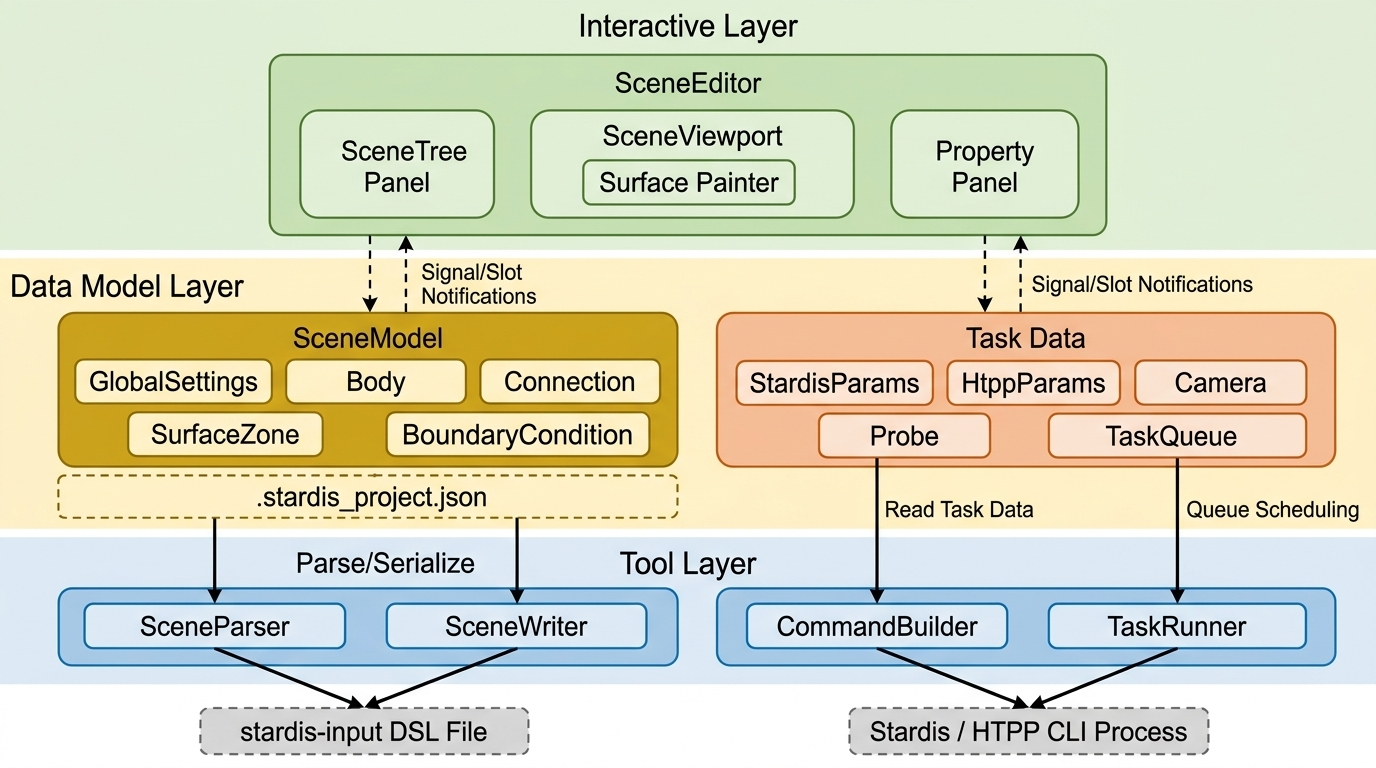
\includegraphics[width=0.9\textwidth]{Figures/editor/architecture/架构.jpg}
  \bicaption{StardisEditor 系统层级架构}{StardisEditor system layer architecture}
  \label{fig:gui:architecture}
\end{figure}

\subsection{工程文件}

编辑器以独立工程文件（\texttt{.stardis\_project.json}）持久化 DSL 之外的编辑器状态：表面区域到介质体的归属映射、区域序号池、画笔标注的面片集、探针/摄像机/灯光位姿、任务队列配置和编辑器版本号。工程文件与 DSL 场景文件共同构成完整的工程描述，支持一键恢复上次工作状态。


%% ============================================================
\section{功能模块设计与实现}
\label{sec:gui:modules}

\subsection{DSL 解析与写出}
\label{sec:gui:parser}

本模块实现 \texttt{stardis-input} DSL 具体语法与内存语义模型 \texttt{SceneModel} 之间的双向转换，是系统全部功能的数据基础。

\subsubsection{语义模型}

\texttt{SceneModel} 是 DSL 的抽象语义表示。其类层次直接对应 DSL 文法中的产生式类别：根对象持有 \texttt{GlobalSettings}（对应 $\langle\text{scaling}\rangle$ 和 $\langle\text{rad-env}\rangle$）、\texttt{Body} 列表（对应 $\langle\text{medium}\rangle$）、\texttt{Connection} 列表（对应 $\langle\text{connection}\rangle$）。每个 \texttt{Body} 下挂载 \texttt{SurfaceZone} 列表，其边界条件对象按 DSL 文法分为四种子类，与 $\langle\text{boundary-condition}\rangle$ 的四类展开式一一对应：\texttt{TemperatureBC}（Dirichlet）、\texttt{ConvectionBC}（Robin）、\texttt{FluxBC}（Neumann）和 \texttt{CombinedBC}（Robin-Neumann）。

\texttt{SurfaceZone} 的区域来源（\texttt{SurfaceZoneSource}）为联合类型：\texttt{ImportedSTL}（来自外部 STL 文件引用，与 DSL 的 $\langle\text{triangles}\rangle ::= \langle\text{stl-path}\rangle$ 直接对应）或 \texttt{PaintedRegion}（来自画笔标注，持有面片 ID 集合——属于编辑器的扩展语义，无 DSL 对应产生式）。

\subsubsection{解析器}

\texttt{SceneParser} 采用逐行分词、关键字分发的策略，按 DSL 文法的终结符（\texttt{SOLID}、\texttt{FLUID}、\texttt{T\_BOUNDARY\_\linebreak[0]FOR\_SOLID}、\texttt{H\_BOUNDARY\_FOR\_SOLID}、\texttt{F\_BOUNDARY\_FOR\_SOLID}、\texttt{HF\_BOUNDARY\_\linebreak[0]FOR\_SOLID}、\texttt{SOLID\_FLUID\_CONNECTION}、\texttt{SOLID\_SOLID\_CONNECTION}、\texttt{TRAD}、\texttt{SCALE}、\texttt{SPHERICAL\_SOURCE} 等）路由到对应的产生式解析函数，按位置顺序提取参数并构造类型化的语义模型对象。

解析流程的关键环节是边界归属的语义分析。如 \ref{sec:gui:dsl} 所述，DSL 中边界条件到介质体的归属关系是隐式的——边界条件行仅声明 STL 文件路径，不显式指定所属介质体名称。解析器通过三级策略依次尝试归属解析：（1）从工程文件的 \texttt{zone\_parent\_map} 做确定性匹配，保证工程重开时归属关系完全还原；（2）基于 STL 文件名前缀的启发式匹配，适用于首次打开的场景；（3）单介质体场景直接归入唯一介质体，多介质体场景将无法确定归属的边界条件标记为 \texttt{unresolved}，由编辑器弹出对话框让用户手动确认。

\subsubsection{写出器}

\texttt{SceneWriter} 将语义模型序列化回合法的 \texttt{stardis-input} 文本。写出时按文法产生式逐类生成描述行：\texttt{SCALE} 行、\texttt{TRAD} 行、各 \texttt{SOLID}/\texttt{FLUID} 行、边界条件行和连接行。对于画笔标注产生的 \texttt{PaintedRegion} 类型区域（不在 DSL 原生表达范围内），写出器调用 VTK 过滤管线（\texttt{vtkThreshold} $\rightarrow$ \texttt{vtkDataSetSurfaceFilter} $\rightarrow$ \texttt{vtkSTLWriter}）将标注面片集导出为独立 STL 文件，再在描述行中以标准 $\langle\text{stl-path}\rangle$ 语法引用该文件，从而将编辑器扩展语义无缝映射回 DSL 的合法表达。

\subsection{三维场景可视化}
\label{sec:gui:viewport}

\texttt{stardis-input} DSL 描述的几何信息仅以 STL 文件路径形式存在，纯文本编辑无法直观呈现几何体的空间关系和法线朝向。本模块（\texttt{SceneViewport}）基于 VTK 渲染引擎为 DSL 的几何语义提供三维可视化投射。

每个 \texttt{Body} 对应一组独立的 VTK 渲染对象（\texttt{vtkSTLReader} $\!\rightarrow\!$ \texttt{vtkPolyDataMapper} $\!\rightarrow\!$ \texttt{vtkActor}），支持独立控制颜色、透明度和可见性。法线可视化功能（\texttt{vtkPolyData\-Normals}）可即时检查面法线朝向，辅助用户确认 DSL 中 $\langle\text{side-specifier}\rangle$（\texttt{FRONT}/\hskip0pt\texttt{BACK}/\hskip0pt\texttt{BOTH}）的正确配置。探针以球体 Actor、IR 摄像机以锥体 Actor 在视口中标示位置与方向。

视口提供导航模式与画笔模式两种互斥交互状态。导航模式下，鼠标响应轨道旋转、平移和缩放；画笔模式下，左键和拖拽事件被路由到 \texttt{SurfacePainter}（\ref{sec:gui:painter}）进行表面区域标注，中键仍可调整观察视角。进入画笔模式时，目标介质体以实体 + 线框叠加显示，其余介质体透明度降低。

图~\ref{fig:gui:viewport} 展示了三维视口的导航模式界面。视口中加载了多个介质体几何。

\begin{figure}[htbp]
  \centering
  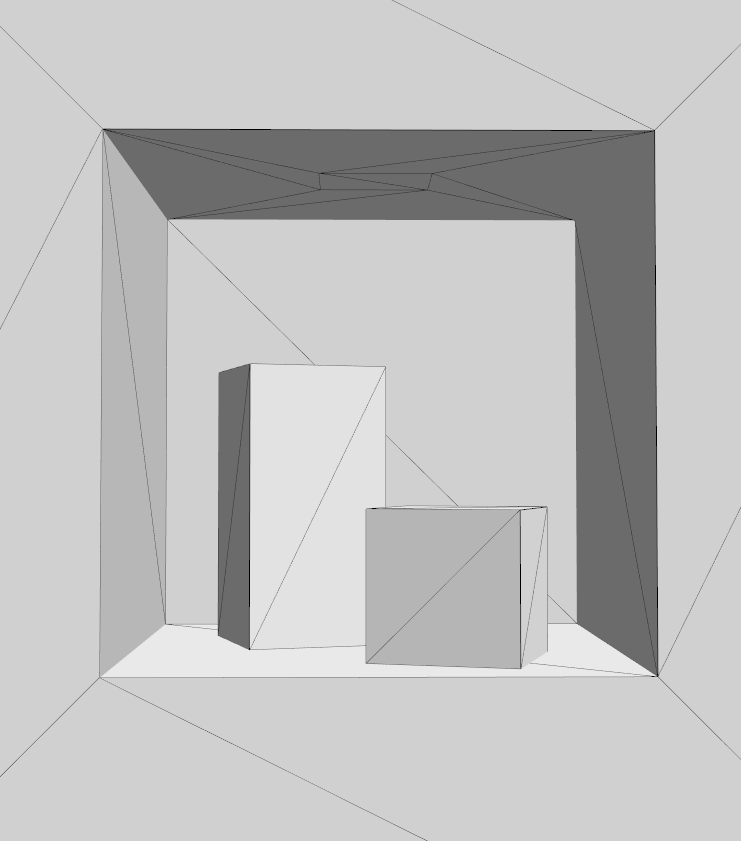
\includegraphics[width=0.65\textwidth]{Figures/editor/panels/VtkNavMode.png}
  \bicaption{三维场景视口：导航模式下的几何体可视化}{3D scene viewport: geometry visualization in navigation mode}
  \label{fig:gui:viewport}
\end{figure}

\subsection{交互式表面区域标注}
\label{sec:gui:painter}

如 \ref{sec:gui:dsl} 所述，DSL 的 $\langle\text{boundary-condition}\rangle$ 产生式要求每条边界条件通过 $\langle\text{triangles}\rangle$ 引用预先分割好的 STL 文件。当同一几何体表面需要划分为多个具有不同换热参数的子区域时，用户必须借助外部三维建模工具切割 STL 并分别导出。本模块（\texttt{SurfacePainter}）通过交互式画笔标注扩展了 DSL 在表面分区方面的能力——标注结果由写出器自动导出为独立 STL 文件并以 $\langle\text{stl-path}\rangle$ 引用，对求解器透明。

\subsubsection{数据结构}

\texttt{SurfacePainter} 在目标介质体的 \texttt{vtkPolyData} 单元数据中附加 \texttt{vtkIntArray}（字段名 \texttt{BoundaryLabel}），记录每个三角面片的区域归属编号（零值表示未归属）。每个面片至多属于一个 \texttt{SurfaceZone}，赋标签时自动从其他区域移除。

\subsubsection{标注操作}

画笔模式下使用 \texttt{vtkHardwareSelector} 执行矩形区域硬件拾取——在拾取通道中以颜色编码渲染场景，通过帧缓冲区获取目标矩形内命中的 Cell ID。提供四种标注操作：
\begin{itemize}
  \item \texttt{BRUSH}（画刷）：屏幕空间拖拽画刷，批量拾取并赋标签；
  \item \texttt{FLOOD\_FILL}（洪泛填充）：从点击面片出发，沿共享边进行 BFS 扩展到连通区域；
  \item \texttt{FILL\_ALL}（全部填充）：将介质体全部面片赋给当前区域；
  \item \texttt{REPLACE\_FILL}（全局替换）：将与点击面片同标签的所有面片改为当前区域。
\end{itemize}

每次落笔前将当前标注数组深拷贝压入撤销栈（最大深度 50），支持完整的撤销/重做操作。

图~\ref{fig:gui:painter} 展示了画笔模式下的表面区域标注过程，不同颜色标识不同边界条件区域。

\begin{figure}[htbp]
  \centering
  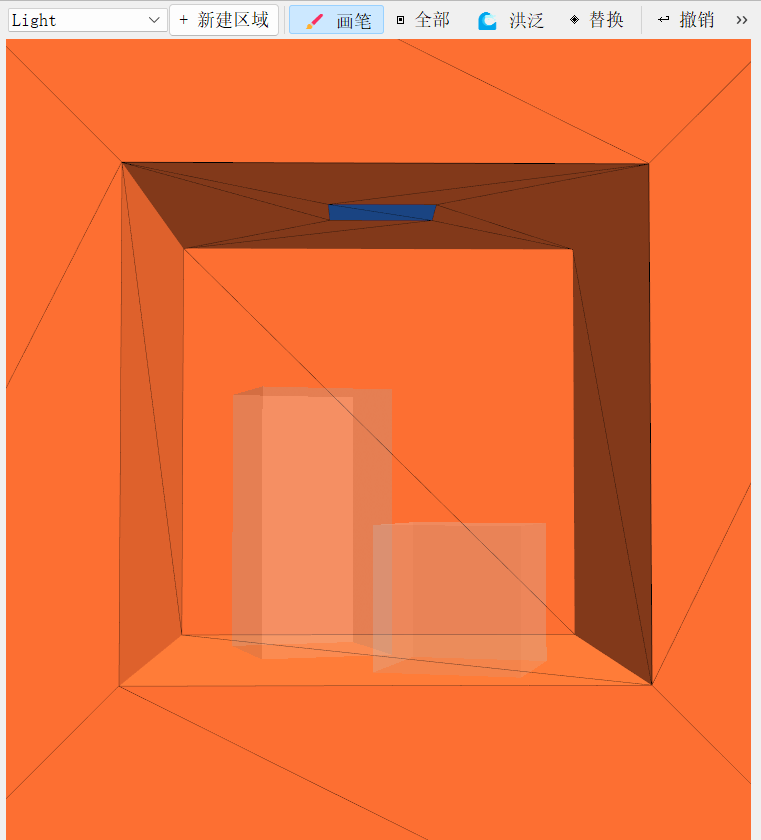
\includegraphics[width=0.65\textwidth]{Figures/editor/panels/VtkPaintMode.png}
  \bicaption{画笔模式下的交互式表面区域标注}{Interactive surface zone annotation in paint mode}
  \label{fig:gui:painter}
\end{figure}

\subsection{场景树与属性编辑}
\label{sec:gui:treeprop}

\texttt{SceneTreePanel} 以层级树形式投射语义模型的完整结构，树节点按类型分组：全局设置、几何体（各 \texttt{Body} 下挂载 \texttt{SurfaceZone}）、连接、探针、摄像机、光源和任务队列。表面区域节点按边界条件类型着色，便于快速识别 Dirichlet/Robin/Neumann/混合边界的分布。

\texttt{PropertyPanel} 根据当前选中节点类型动态切换对应属性编辑器：
\begin{itemize}
  \item \texttt{BodyEditor}：编辑 DSL $\langle\text{medium}\rangle$ 产生式的全部参数——介质类型、$\lambda$、$\rho$、$c_p$、$\delta$、$T_{\rm init}$、$T_{\rm imposed}$、体积热源功率、$\langle\text{side-specifier}\rangle$，以及该介质体的表面区域列表；
  \item \texttt{SurfaceZoneEditor}：编辑 DSL $\langle\text{boundary-condition}\rangle$ 各展开式的参数——Dirichlet 型（$T$）、Robin 型（$T_{\rm ref}$、$\varepsilon$、$f_s$、$h_c$、$T_{\rm env}$）、Neumann 型（$\Phi$）和混合型；
  \item \texttt{ConnectionEditor}：编辑 DSL $\langle\text{connection}\rangle$ 的参数（固-流连接或固-固连接的接触热阻）；
  \item \texttt{CameraEditor}、\texttt{ProbeEditor}、\texttt{LightEditor}：编辑 DSL 不涉及但仿真任务所需的场景对象（IR 摄像机位姿、探针坐标、灯光参数）。
\end{itemize}

属性编辑器的修改通过信号/槽链路写回 \texttt{SceneModel}，主窗口随后重建场景树并刷新视口。

图~\ref{fig:gui:treeprop} 展示了场景树与属性面板的联动界面，选中某一介质体时属性面板自动切换显示对应参数编辑器。

\begin{figure}[htbp]
  \centering
  \begin{subcaptiongroup}
  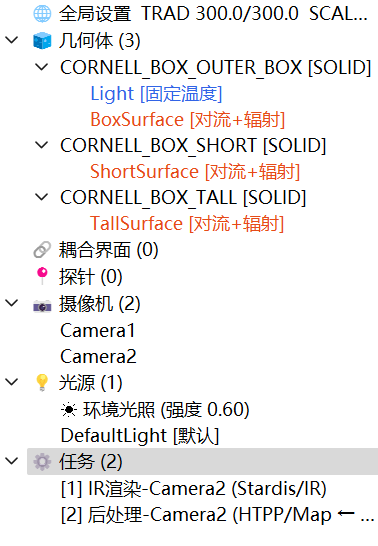
\includegraphics[height=0.42\textheight]{Figures/editor/panels/SceneTree.png}
  \hfill
  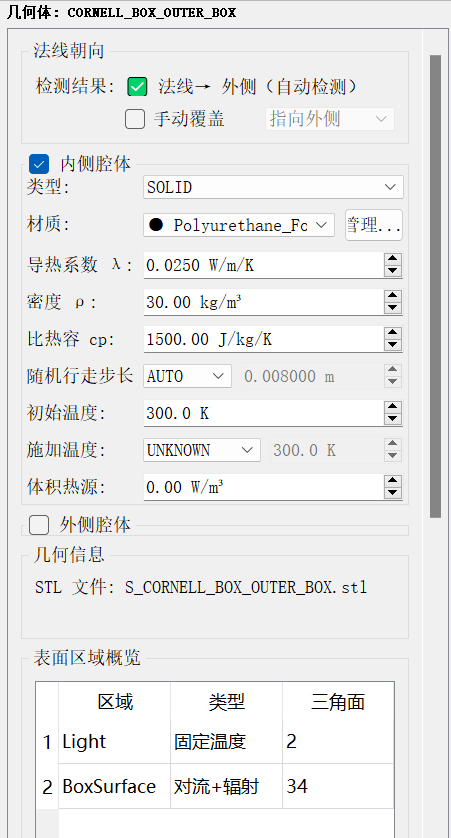
\includegraphics[height=0.42\textheight]{Figures/editor/panels/GeometryMeshConfig.png}
  \end{subcaptiongroup}
  \bicaption{场景树（左）与几何体属性编辑面板（右）}{Scene tree (left) and geometry property editor panel (right)}
  \label{fig:gui:treeprop}
\end{figure}

\subsection{仿真任务配置与执行}
\label{sec:gui:taskrunner}

Stardis CLI 的运行时参数（采样数、渲染分辨率、探针坐标等）和后处理工具 HTPP 的参数均不属于 \texttt{stardis-input} DSL 的定义范围。本模块将这些运行时参数结构化管理，以图形化界面替代手动命令行拼接。

\texttt{CommandBuilder} 将 \texttt{Task} 数据对象转换为可执行的 CLI 参数列表。任务通过名称引用 \texttt{SceneModel} 中的场景对象（如摄像机名称、探针名称列表），而非硬编码路径和数值。执行前由 \texttt{resolve\_all()} 将名称引用求值为实际 CLI 参数，确保场景编辑后重新执行时始终使用最新数据。HTPP 任务的输入文件同样通过引用队列中的 Stardis 任务输出来解析，避免硬编码路径。

\texttt{TaskRunner} 以 PyQt5 \texttt{QProcess} 管理子进程生命周期，在主线程事件循环中通过信号接收进程输出，日志面板实时更新。队列中的任务顺序执行；任务异常退出时按错误策略自动重试、跳过或暂停等待用户介入。

编辑器的偏好设置中，用户可将多个 Stardis/HTPP 可执行文件路径命名为标签（如 \texttt{CPU-Release}、\texttt{GPU-Release}），任务配置通过标签名引用——同一任务配置可通过切换标签在不同求解器版本间切换，直接对应第三、四章实验中的 CPU 基线与 GPU 加速版本选择。

图~\ref{fig:gui:taskrunner} 展示了任务配置与执行界面。左图为 Stardis IR 渲染任务的参数配置面板，设定了线程数、传导算法和摄像机引用等运行参数；中图为 IR 摄像机参数面板，设定了位姿、视场角、每像素采样数（SPP）和分辨率——IR 渲染模式下，图像分辨率与采样数由摄像机参数决定，而非任务面板中的样本数字段；右图为任务队列面板与实时运行日志。

\begin{figure}[htbp]
  \centering
  \begin{subcaptiongroup}
  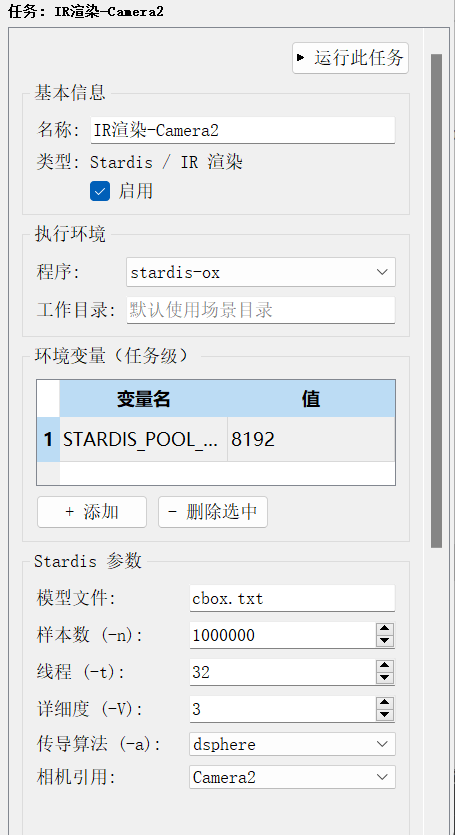
\includegraphics[height=0.4\textheight]{Figures/editor/panels/StardisConfig.png}
  \hfill
  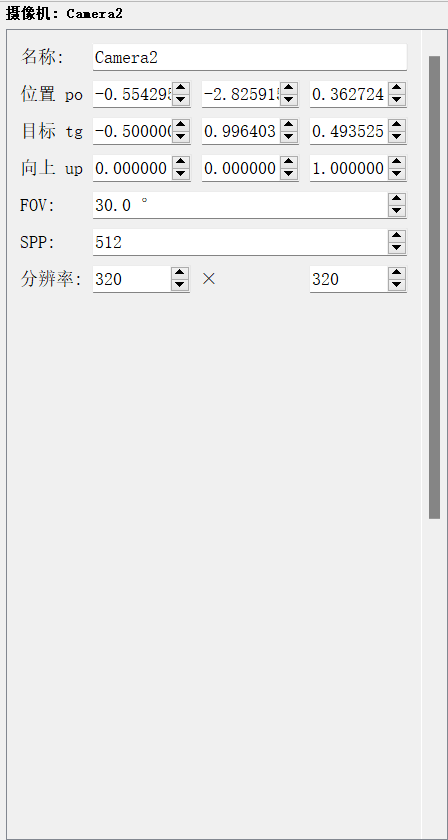
\includegraphics[height=0.4\textheight]{Figures/editor/panels/CameraConfig.png}
  \hfill
  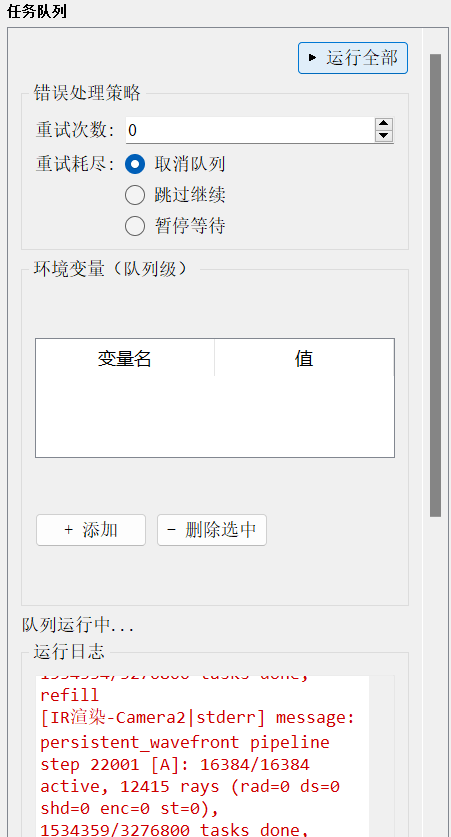
\includegraphics[height=0.4\textheight]{Figures/editor/panels/TaskQueue.png}
  \end{subcaptiongroup}
  \bicaption{Stardis 任务配置与执行界面}{Stardis task configuration and execution interface}
  \label{fig:gui:taskrunner}

  \small
  任务配置面板（左）、IR 摄像机参数面板（中）与任务队列面板（右）。
\end{figure}


%% ============================================================
\section{应用案例}
\label{sec:gui:cases}

本节以 Cornell Box 热仿真场景为例，演示从几何导入到仿真结果的完整工作流。经典 Cornell Box 场景以封闭空腔与内部几何体构成多次反射环境，广泛用于全局光照算法验证；类似地，本场景呈现多个导热体在封闭空间内，受顶部定温热源的辐射照射，在辐射、传导和对流三种耦合热输运过程共同作用下，达到稳态热平衡的红外仿真结果。

\subsection{场景描述}

场景包含三个 SOLID 介质体（图~\ref{fig:gui:case-import}）：外层盒体 \texttt{CORNELL\_BOX\_OUTER}（36 个三角面片）及内部两个长方体 \texttt{CORNELL\_BOX\_SHORT}（12 面片）和 \texttt{CORNELL\_BOX\_TALL}（12 面片），三者均以聚氨酯泡沫（Polyurethane Foam，$\lambda = 0.025\;\text{W/(m·K)}$，$\rho = 30\;\text{kg/m}^3$，$c_p = 1500\;\text{J/(kg·K)}$）为介质材料，初始温度 $T_{\rm init} = 300\;\text{K}$。

\begin{figure}[htbp]
  \centering
  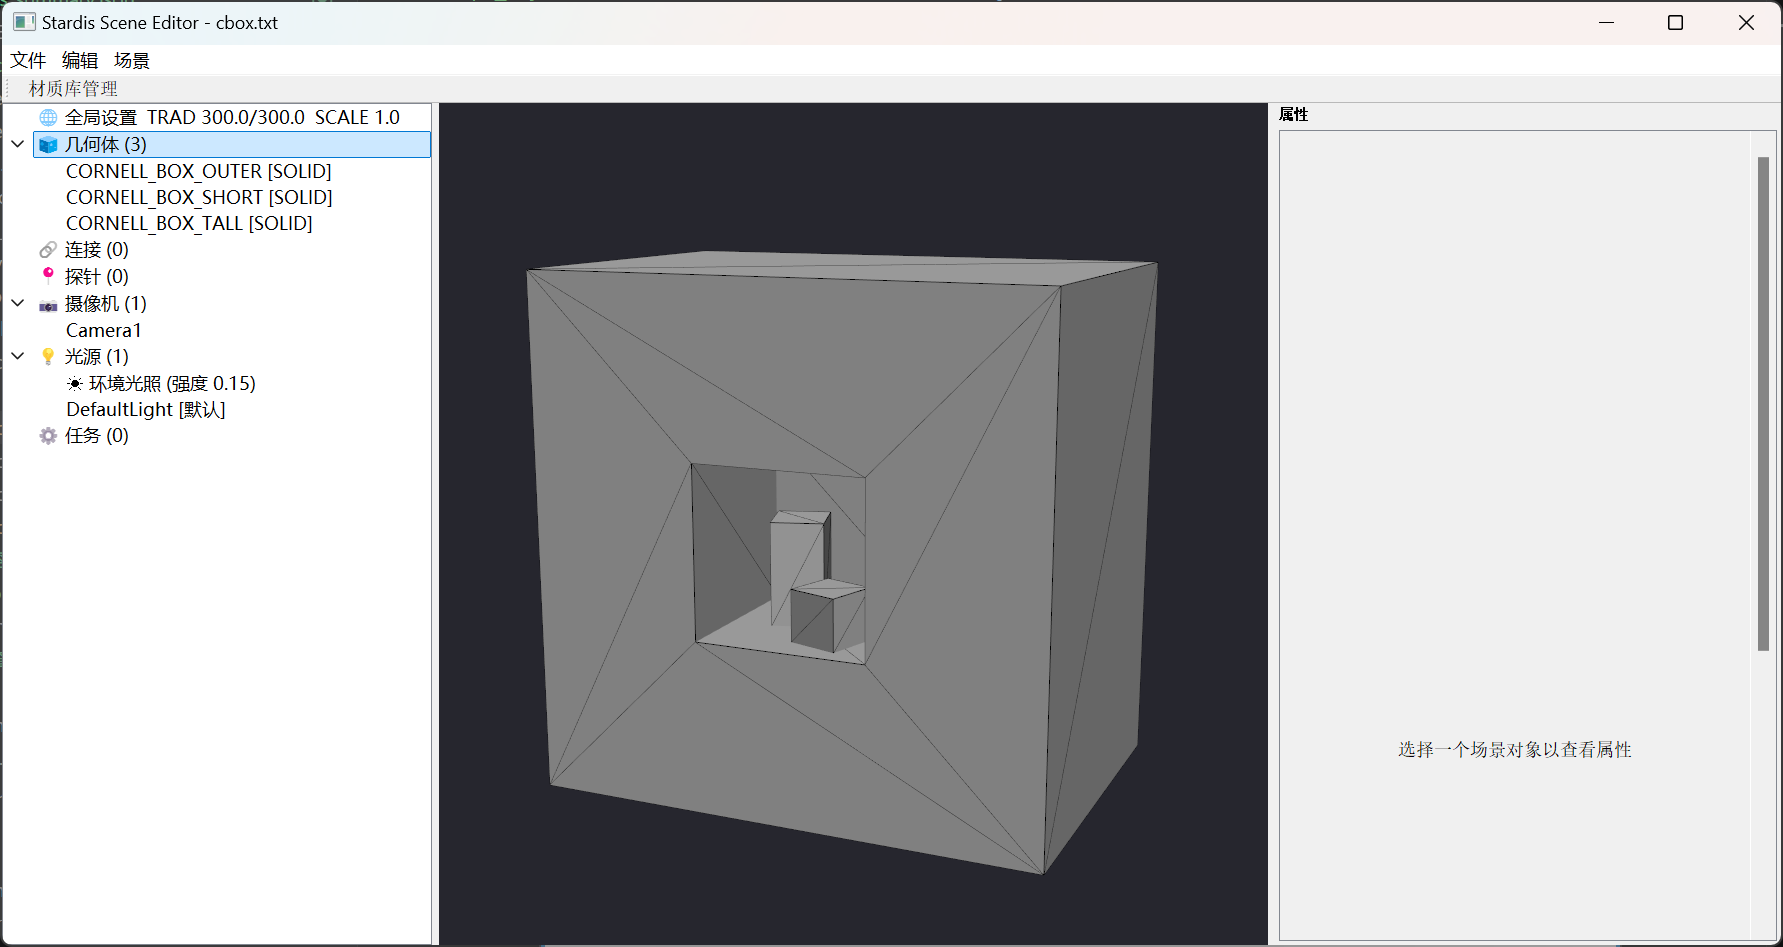
\includegraphics[width=0.85\textwidth]{Figures/editor/workflow/1_2_ImportedGeometry.png}
  \bicaption{Cornell Box 场景几何导入结果：三个 SOLID 介质体}{Cornell Box scene after geometry import: three SOLID media bodies}
  \label{fig:gui:case-import}
\end{figure}

\subsection{边界条件标注与任务配置}

利用画笔标注模块（\ref{sec:gui:painter}），在外层盒体表面划分两个边界条件区域：顶部 2 个面片标注为 \texttt{Light}（Dirichlet 型，$T = 1000\;\text{K}$），代表定温热源；其余 34 个面片标注为 \texttt{BoxSurface}（Robin 型，$\varepsilon = 0.9$，$h_c = 10\;\text{W/(m}^2\text{·K)}$，$T_{\rm env} = 300\;\text{K}$），代表与外部环境的对流-辐射耦合换热。两个内部长方体表面分别整体标注为 \texttt{ShortSurface} 和 \texttt{TallSurface}，边界条件类型与外壁相同。标注完成后，画笔模块自动为每个区域导出独立的 STL 文件供求解器引用。

图~\ref{fig:gui:case-paint-config} 展示了画笔标注与任务配置。左图为外层盒体的画笔标注结果，橙色区域为具有对流-辐射耦合换热的一般固体表面（\texttt{BoxSurface}，Robin 型，$\varepsilon = 0.9$，$h_c = 10\;\text{W/(m}^2\text{·K)}$），蓝色面片为顶部热源区域（\texttt{Light}，Dirichlet 型，$T = 1000\;\text{K}$）；右图为 Stardis IR 渲染任务的参数配置，设定了 32 线程、\texttt{dsphere} 传导算法，并通过 Camera2 的名称引用自动获取摄像机位姿与渲染参数（位姿、SPP、分辨率等，见图~\ref{fig:gui:taskrunner} 中图）。

\begin{figure}[htbp]
  \centering
  \begin{subcaptiongroup}
  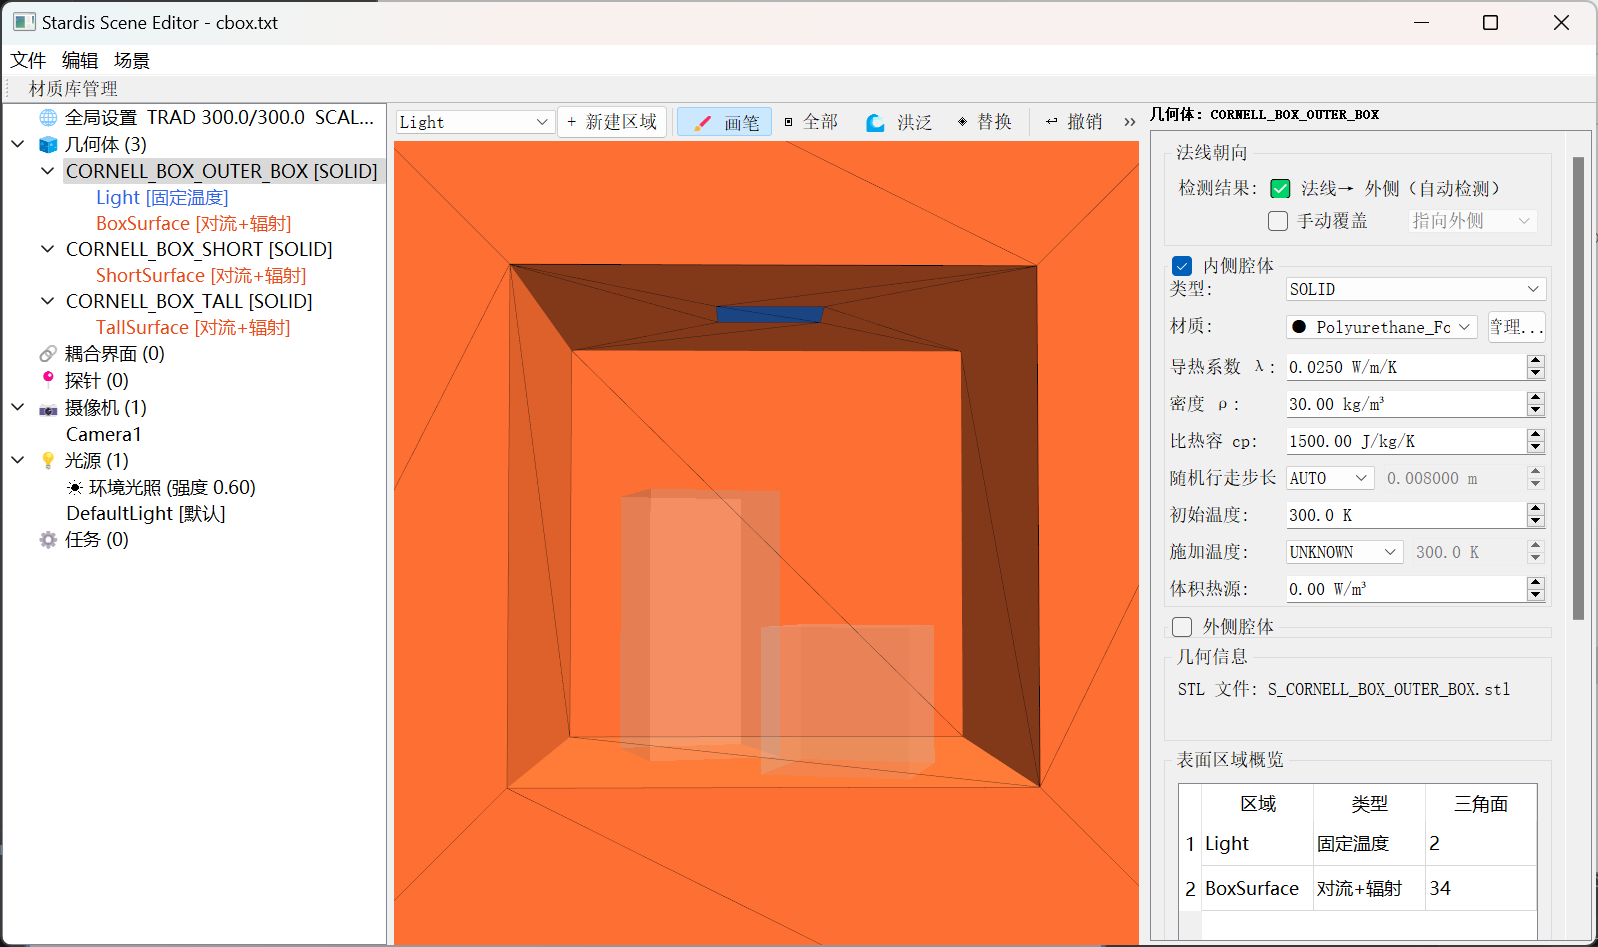
\includegraphics[width=0.48\textwidth]{Figures/editor/workflow/3_1_PaintBNDCondition.png}
  \hfill
  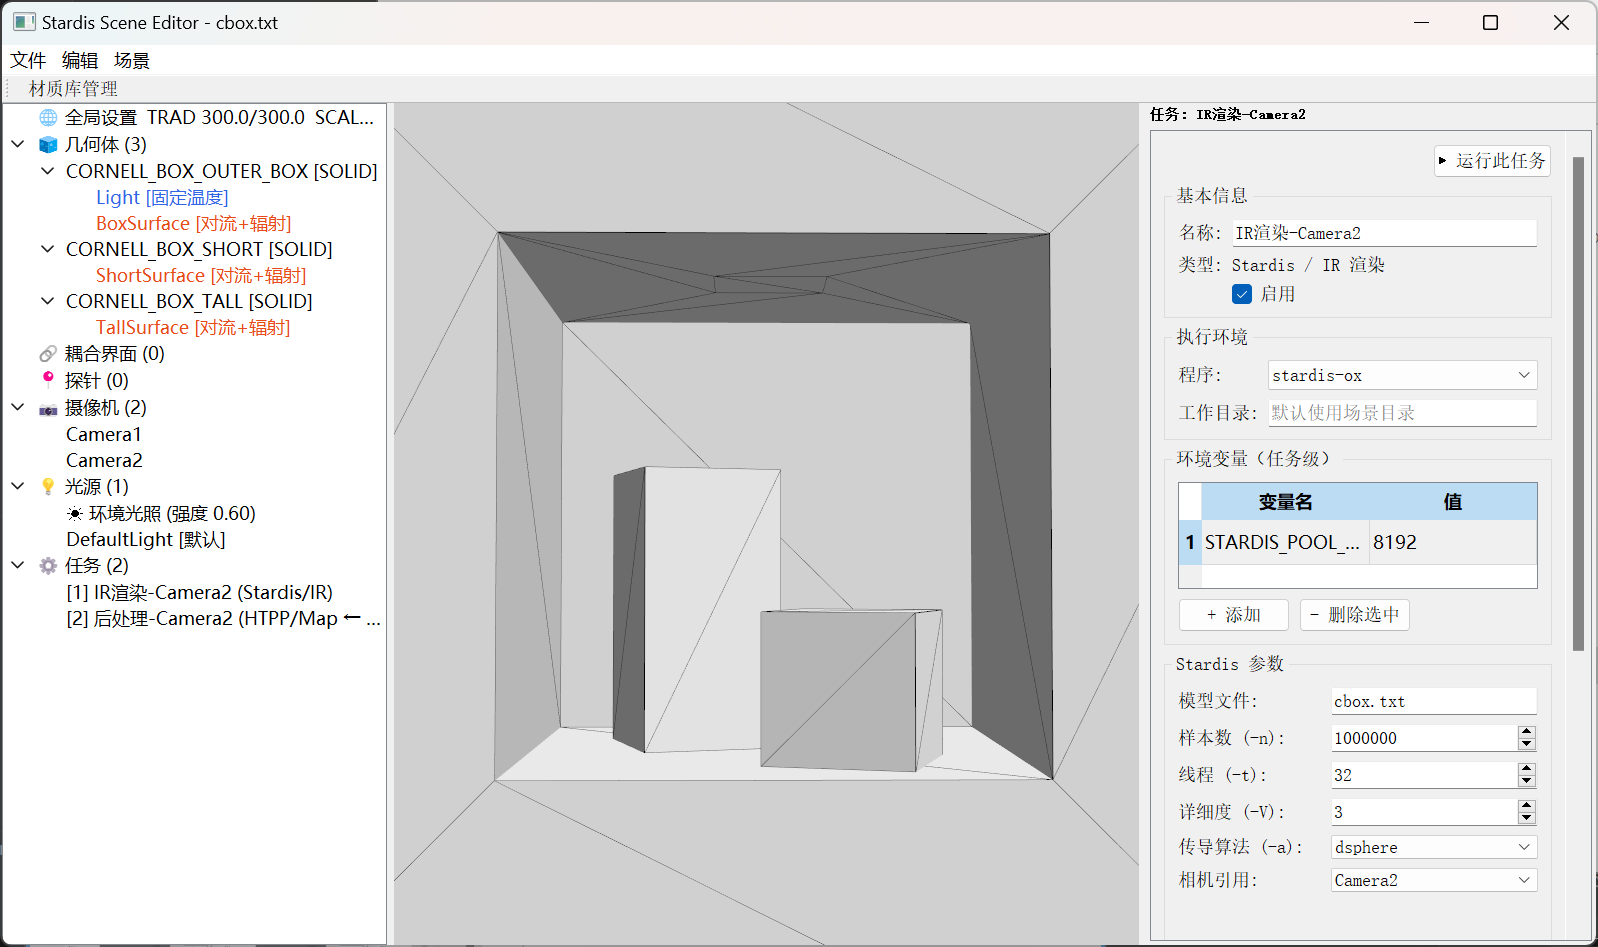
\includegraphics[width=0.48\textwidth]{Figures/editor/workflow/6_1_ConfigTask.png}
  \end{subcaptiongroup}
  \bicaption{外层盒体画笔标注（左）与 Stardis IR 渲染任务配置（右）}{Outer box boundary annotation (left) and Stardis IR rendering task configuration (right)}
  \label{fig:gui:case-paint-config}
\end{figure}

\subsection{仿真执行与结果}

任务队列依次执行 Stardis IR 渲染和 HTPP 后处理（色调映射）。运行日志面板实时显示 Wavefront 管线的迭代进度（如 \texttt{step 22001, 16384/16384 active}）。图~\ref{fig:gui:case-result} 为稳态热平衡下的红外仿真结果：顶部热源（$1000\;\text{K}$）呈高亮，盒体内壁因多次辐射反射和传导扩散产生连续温度梯度，两个内部长方体因较低导热系数呈现明显低温区域，整体温度场分布符合辐射-传导-对流耦合输运的物理预期。

\begin{figure}[htbp]
  \centering
  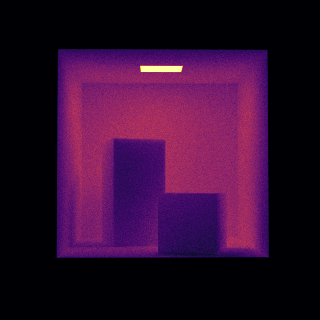
\includegraphics[width=0.45\textwidth]{Figures/editor/workflow/8_Result.png}
  \bicaption{Cornell Box 稳态红外仿真结果（inferno 色调映射）}{Cornell Box steady-state IR simulation result (inferno colormap)}
  \label{fig:gui:case-result}
\end{figure}

该案例展示了从 DSL 场景构建到红外仿真输出的完整闭环：几何导入与三维预览验证空间关系 → 画笔标注划分边界条件区域 → 属性编辑设定物理参数 → 任务配置引用场景对象 → 队列化执行与实时日志监控 → 后处理色调映射可视化。全部操作在 StardisEditor 内完成，无需手动编辑 DSL 文本或拼接命令行参数。

%% ============================================================
\section{小结}
\label{sec:gui:summary}

本章以 \texttt{stardis-input} 领域描述语言的形式文法为基础，设计并实现了 GUI 场景编辑器 StardisEditor。在 DSL 工具链层面，编辑器实现了语法感知的解析与写出闭环——\texttt{SceneParser} 按 BNF 文法将 DSL 文本解析为类型化语义模型 \texttt{SceneModel}，\texttt{SceneWriter} 将编辑后的模型序列化回合法 DSL 文本，包括将画笔标注的扩展语义自动映射为标准 STL 引用。在 DSL 表达能力之外，编辑器提供了三项关键扩展：基于 VTK 的三维几何可视化使空间关系和法线朝向直观可见；交互式画笔标注使表面区域划分无需借助外部建模工具；结构化任务配置与队列化执行替代了手动命令行拼接。可执行文件标签引用机制使任务配置在求解器版本管理层面联通了第三章 Wavefront 求解器和第四章 OptiX 后端的对比实验场景。

至此，论文完成了 Wavefront 并行化求解器（第三章）、OptiX GPU 光追后端（第四章）和场景编辑器（本章）三个核心贡献的阐述；第六章将对全文研究工作进行总结并展望未来研究方向。

%!TEX root = ../MainBody.tex

\chapter{总结与展望}

\section{总结}

基于路径追踪的蒙特卡洛方法为耦合热输运红外仿真提供了一条无需空间网格化的求解途径，可在同一路径空间中同时处理辐射、传导、对流三类耦合热输运过程。然而，该方法在实际仿真规模下面临严峻的计算效率挑战：单条路径在完整生命周期内需执行数十万次异构几何查询，每个探测器像素需数百条独立路径以达到工程收敛精度，总查询量达数十亿量级。原始 CPU 逐路径的递归路径追踪求解架构以同步阻塞方式逐条执行几何查询，无法利用 GPU 大规模并行吞吐能力。本文针对上述问题，以 Wavefront 等价变换为核心，设计了面向 GPU 加速的并行化耦合热输运红外仿真架构，并以 CPU-GPU 混合方式完成首个工程实例化与正确性验证，包含三项主要贡献。

\paragraph{ 基于 Wavefront 架构的并行化耦合热输运求解器}（第三章）。本文提出了将递归求解器等价改造为耦合输运状态机Wavefront求解器的完整方法。首先，从并行化设计视角对原始算法进行规约分析，识别出全部 19 个几何查询挂起点、三类不可消除的查询类型（RT 射线求交、CP 最近面投影、ENC 封闭腔体成员判定）以及五类路径状态字段，为状态机设计提供完备约束。在此基础上，通过递归到状态机的等价变换，将路径状态从函数调用栈显式化为持久化 \texttt{path\_state} 结构体，解耦状态推进与几何查询执行，构建了以路径池为中心的 Wavefront 四阶段迭代执行模型（推进$\to$收集$\to$批量执行$\to$回填）。工程实现上，设计了 CPU 承担路径调度、GPU 承担批量查询的混合架构，并引入双流 Ping-Pong 异步调度机制以隐藏跨设备传输延迟。实验验证方面，物理过程一致性验证覆盖 13 个递进复杂度的验证场景，共计 282 个有效数据点全部通过 $3\sigma$ 检验；端到端统计等价性检验在 porous 场景上对 153{,}976 个有效像素执行逐像素双样本 $Z$ 检验，经 Bonferroni 和 Benjamini-Hochberg 双重多重比较校正后报告零显著差异像素，确认 Wavefront 改造不引入系统性偏差。性能实验表明，32 线程下 Wavefront求解器+OptiX 方案与递归求解器+Embree 基线达到性能均势（$1.02\times$），8\textasciitilde 16 线程典型工作站配置下实现 $1.3$\textasciitilde$1.4\times$ 端到端加速；路径池容量对比实验（8{,}192 $\to$ 16{,}384，$2.25\times$ 退化）与查询后端消融实验（WF + Embree 单池 = 426~s，Baseline 的 $4.0\times$ 退化）共同定量证明 CPU 侧 Cache Miss 为当前主导性能约束、GPU 后端是恢复性能均势的必要条件，为后续优化提供了明确方向。

\paragraph{ 基于 OptiX 的 GPU 硬件光追查询后端}（第四章）。针对 Wavefront 架构产生的三类批量查询请求，本文设计了基于 NVIDIA OptiX 的统一 GPU 查询后端。RT 查询作为硬件光追的原生操作，由 RT Core 直接加速 BVH 遍历与三角形求交，在 RTX 4090 平台上实测吞吐达 5.15 GRays/s，约为 CPU Embree 后端（i9-13900K，16 线程，15.45 MRays/s）的 333 倍。CP 查询在语义上不是射线问题——\texttt{optixTrace()} 返回射线-三角形交点而非查询点到三角形的投影点——本文通过自定义 AABB 图元代理与零长射线相结合的方法，将近接投影查询重构为等价的光追问题，实现 19.7\textasciitilde 45.9 倍 GPU/CPU 加速。ENC 查询基于 Jordan-Brouwer 分离定理，将多面体点-内外关系判定分解为一次 CP 查询与一条 $+X$ 方向射线查询的组合，仅需两次 \texttt{optixLaunch} 即完成。三类映射整合于单一 OptiX Pipeline 中，通过五套 Shader Binding Table 实现查询类型路由，后端接口与原 Embree 后端 100\% API 兼容，支持受控对比实验。

\paragraph{ 热输运场景仿真任务 GUI 编辑器}（第五章）。作为面向仿真工作流的配套工程工具，针对 Stardis 求解器纯命令行接口在场景文件手工编辑、几何缺乏可视化、表面区域手工对应、任务参数组装繁琐、多任务缺乏自动化五类系统性使用痛点，本文设计并实现了基于 Python 3 + PyQt5 + VTK 的图形化编辑器 StardisEditor。编辑器提供场景文件完整读写闭环、三维可视化与交互式画笔标注、场景树层级浏览与属性编辑、任务队列配置与自动化执行等功能，以工程文件格式统一管理场景与任务配置。Model-View 架构与信号/槽机制保证多面板间数据一致性，可执行文件标签引用机制从工作流层面联通了 Wavefront 求解器与 OptiX 后端的对比实验。

综上，本文三项贡献共同构成了从求解器内核改造、GPU 查询后端设计到用户工具链建设的完整技术体系。Wavefront 架构实现了路径状态与几何查询的解耦，为批量化 GPU 加速提供了架构基础；OptiX 后端将三类异构查询统一映射至 GPU 硬件光追管线，在关键查询类型上实现了两到三个数量级的吞吐提升；GUI 编辑器作为配套工程工具将上述算法能力封装为可重复、低门槛的工程实践。物理一致性验证与端到端统计等价性检验共同确认，混合架构在实现性能提升的同时不引入系统性物理偏差。上述成果有效验证了 Wavefront 架构的正确性与查询后端的吞吐能力，同时精确定位了 CPU 侧实现的性能天花板，为全 GPU 架构演进提供了明确的实验依据。系统化的几何敏感性与超大规模场景扩展性验证留待后续工作。

\section{工作展望}

尽管本文在 Wavefront 并行化架构、GPU 光追后端和 GUI 工具链三个方面取得了阶段性成果，当前系统仍存在若干局限性，可从以下方向展开后续研究。

\subsection{ 全 GPU 求解器架构 }当前混合架构中，路径状态调度（advance/cascade/distribute）保留在 CPU 侧执行，$T_A/T_B$ 时间分解（表~3.6）显示 GPU 设备侧仅占墙钟时间的 10.9\%，端到端加速上界仅为 $1.12\times$；路径池容量从 8{,}192 增至 16{,}384 即引发 $2.25\times$ 性能退化（第三章 3.4.3）。消除该瓶颈的根本途径是将路径状态调度整体迁至 GPU ，并在 GPU 端原生组织 Wavefront 执行模型。全 GPU 求解还可消除显式 \texttt{optixLaunch} 在每轮迭代间产生的 host 端 kernel 启动开销；查询经由 OptiX 内联接口（\texttt{optixTraverse} / \texttt{optixReportIntersection}）在调度 kernel 内直接发起，使 FSM 状态推进与查询执行融合为同一指令流。

全 GPU 路线的核心工程难点在于 GPU 端调度内核的实现。调度内核主要由 Wavefront 、FSM 和更底层的场景物理信息访问函数组成。在 Wavefront 层，调度本身不再是 CPU 主控的批次循环，而是 GPU 上的持久线程网格：每个 warp 持续从路径池消费 active 路径，完成“状态推进 $\to$ 查询发起 $\to$ 结果写回”的全过程；由于 FSM 的数十个状态在同一 warp 的 32 个 lane 内极可能高度分歧、直接执行会显著拉低 SIMT 利用率，可借鉴现代高性能 Wavefront 路径追踪器的成熟做法，在每轮推进前以 stream compaction 按状态 ID 对 active 路径重排，使 warp 内 lane 状态同质化以提高一致性。在 FSM 层，本文混合架构所定义的 \texttt{path\_state} 需进一步推进 SoA 化，使 advance 阶段对热字段的访问由 lane 级分散读写转换为 warp 级合并访存；由于 GPU 实现无需在几何查询处挂起，还可将挂起点前后的 FSM 状态融合并将几何查询直接内联，显著减少状态数与跨状态数据搬运，进一步降低线程分歧；此外，本文方法对 PicardN 迭代的求解采用了深度受限显式栈，这在 GPU 端并不适用，但可通过将具有树状关系的路径状态展平为线性结构并以 parent index 进行关联的方式实现等价功能，相关技术细节留待后续工作展开。针对更底层的场景物理信息访问函数，GPU 端实现的主要挑战在于构造与基于函数指针的 CPU 实现等价的高性能抽象接口，以支持多样化的场景几何与热物理模型；经过对这类函数的分析，其遵循统一的调用规约、访问模式高度数据驱动，可直接从绑定在几何上的物理属性数据中读取所需信息。

\subsection{ 借鉴现代高性能路径追踪的工程优化技术 }本文 Wavefront 求解器以耦合热输运的物理正确性为首要目标完成实例化，在调度组织与算法层面仍保有可观的提升空间。现代图形界的高性能路径追踪器（如 NVIDIA Falcor / NRD 体系、商用 DXR 渲染管线）所积累的大量工程优化与本文求解器结构高度同源，可按两条主线在前述全 GPU 实例化基础上有选择地引入。

第一条主线是\emph{warp 同质化}，本质是将“行为相近的路径聚到同一 warp”做到极致。除前述按状态 ID 的 stream compaction 之外，可按事件类型将每轮路径推进进一步拆分为多个独立 kernel（生成、扩展、阴影、交互、终止），使每个 kernel 内 lane 同质性更高；在材质评估阶段对路径按材质 ID 或查询类型做二次排序（Coherent Shading）使同 warp 内 lane 访问相同材质资源；并借助 NVIDIA Shader Execution Reordering（SER）由硬件在 OptiX 内联调用点自动完成 warp 重组。该主线与本文 FSM 的多状态结构天然契合，是前述 Wavefront 层调度内核的延伸优化。

第二条主线是\emph{路径剪枝}，本质是“按贡献裁减低收益路径”。蒙特卡洛路径的能量贡献存在显著长尾，Russian Roulette 与自适应路径长度可在期望意义下保持无偏的同时大幅截断低贡献路径段。该机制与本文耦合热输运框架天然兼容，与调度架构正交，可单独引入并预期在 PicardN 高阶展开与多次散射场景下带来直接收益。

上述两条主线与本文 FSM、\texttt{path\_state}、批量查询接口设计正交，无需对架构作根本性改动即可逐项引入。

\subsection{ 更丰富的物理模型 }本文采用漫射灰体、透明非参与流体与线性化对流系数三条工程简化（见第二章末），覆盖了主流工业红外仿真任务。当假设失效时，所需扩展同时涉及学术与工程两个层面：学术层面关注物理模型在路径空间中的可表达性、蒙特卡洛估计器的无偏性与方差可控性；工程层面关注 FSM 与查询管线的结构改动。两个层面缺一不可。

\emph{参与性介质失效}（烟气、火焰、薄云、气溶胶）。学术上，路径空间从"表面—表面"扩展到"表面—体—表面"，需在路径密度中引入沿光程的指数衰减项 $\exp(-\!\int_0^s \sigma_t(\ell)\,\mathrm d\ell)$ 与散射相函数 $f_p$。估计器无偏性要求自由飞行距离采样严格匹配介质消光系数（如 Woodcock null-collision 跟踪）；散射事件需通过相函数的解析或表式重要性采样保持概率密度归一；多次散射路径的方差控制依赖 Russian Roulette 与 Next-Event Estimation 等成熟方差缩减技术。Bati 等\cite{batiCouplingConductionConvection2023} 单路径框架在原理上已涵盖该方向，但 PicardN 在非线性辐射边界与体积参与项耦合下的收敛性与无偏性需重新分析证明。工程上，FSM 需新增"介质内自由飞行—散射/吸收事件"段落（约 5\textasciitilde 7 个状态），GPU 查询管线需扩展 RT 类型以支持体积光线步进与采样；该类扩展属于结构性改动，但与本文 RT/CP/ENC 三类查询保持正交。

\emph{多光谱辐射失效}（强温度依赖发射率、谱选择性材料、大气吸收带）。学术上，单波段灰体假设失效后，能量沿路径不再由单一频道携带，需在路径空间中引入波长维度；常见处理方式有按光谱发射密度采样的 Spectral Importance Sampling 与 Hero Wavelength + 重要性采样方案，两者在统计上均可保持无偏但方差—成本权衡不同；$\varepsilon(\lambda,T)$ 与 Planck 函数 $B_\lambda(T)$ 在 PicardN 内展开的一致性条件需重新推导。工程上，在 \texttt{path\_state} 中扩展波段索引字段，材质系统由灰体单值扩展为按谱段查表，采样阶段引入波段抽样；FSM 状态拓扑与查询管线本身无需结构性改动。

\emph{强非线性对流系数失效}（自然对流主导、相变换热等）。学术上，线性化对流系数 $h_{cv}=\mathrm{const}$ 在 PicardN 的 null-collision 分支选择中被显式使用以保证概率归一与无偏；若 $h_{cv}=h_{cv}(T)$ 强非线性，需将其作为 PicardN 框架内的非线性项与辐射项 $h_{rd}(T)$ 同等处理，重新推导多温度采样的乘积估计形式；当 $h_{cv}$ 跨越数量级时，估计器方差的可控性需通过 majorant 上界或额外方差缩减手段保证。工程上，在 advance 阶段引入温度依赖的换热系数闭包即可，FSM 与查询管线均保持不变。

总体而言，三类假设失效在学术上的挑战远大于工程上的改动。在学术层面问题得到解决的前提下，工程层面的扩展可在本文 \texttt{path\_state} + 批量查询接口范式内逐步实施。上述扩展的理论分析、原型实现与无偏性验证留待后续工作。

\subsection{ 仿真管线与工业/DCC 软件的数据互通 }当仿真目标从单一构件级算例扩展到整机级或系统级工业场景时，几何资产规模与边界条件复杂度迅速膨胀，单一 GUI 编辑器以手工方式组织几何、材质、边界条件、传感器布置与任务参数已不可持续——编辑管线本身成为新的瓶颈。务实的扩展方向是将本文求解器与编辑器纳入现有工业 / DCC 工具链的数据流，使 StardisEditor 在两个职能维度上从“全功能编辑器”退守为“红外仿真求解 + 结果可视化”节点。

\emph{静态场景数据维度}：将本文 BNF 文法的场景描述以更通用的结构化格式（JSON Schema、USD Schema 等）重表达，作为统一的入口数据契约；其上层资产数据通过中性格式与工业/DCC 生态对接——CAD/CAE 侧由 STEP/IGES、CGNS 等中性格式承担装配级几何与已划分网格的导入，DCC 侧由 USD、glTF、Alembic 等开放资产格式与 Blender、Maya、Houdini 等工具共享几何与光学/热学材质属性。这一维度的核心是让 StardisEditor 退出“建模与材质指派”的职能。

\emph{动态任务流程维度}：把参数扫掠、批处理、不确定度分析等大规模算例的编排能力让渡给更成熟的工作流引擎（如 ParaView、Cassiopée），StardisEditor 仅作为求解任务节点参与编排。这一维度的核心是让 StardisEditor 退出“任务调度”的职能。

在上述两维互通的基础上，交互式预览可作为面向终端用户体验的附属增强保留：结合基于深度学习的蒙特卡洛降噪算法，以低 SPP（如 1\textasciitilde 4）配合实时降噪实现秒级红外预览，使用户在跨工具编辑场景参数时即时获得温度场反馈。

% 设置论文正文后的式样
\backmatter
% 按国标自动制作参考文献
% 参考文献数据文件为本目录下的ReferenceBase.bib
\begin{reference}
	\bibliography{ReferenceBase}
\end{reference}
% 包含在读期间科研成果
%!TEX root = ../MainBody.tex

% 作者在读期间科研成果简介
\chapter{攻读学位期间取得的研究成果}
\ifthenelse{\equal{\approval}{0}}{%
以第二发明人身份（导师第一发明人），撰写专利《一种基于光栅化与路径追踪混合架构的红外场景渲染方法》专利号202511337747.0/已进入实质性审查阶段
}{%
以第二发明人身份（导师第一发明人），撰写专利《******》/实质性审查阶段
}

% 包含致谢
\makethanks
\end{document}
